\documentclass[sigconf]{acmart}

\fancyhf{} % Remove fancy page headers
\fancyhead[C]{Anonymous submission \#399 to ACM CCS 2022} % TODO: replace 9999 with your paper number
\fancyfoot[C]{\thepage}

\setcopyright{none} % No copyright notice required for submissions
\acmConference[Anonymous Submission to ACM CCS 2022]{ACM Conference on Computer and Communications Security}{Due 2 May 2022}{London, TBD}
\acmYear{2022}

\settopmatter{printacmref=false, printccs=true, printfolios=true} % We want page numbers on submissions

\newif\ifWorkInProgress
%\WorkInProgresstrue
\WorkInProgressfalse

%-------------------------------------------------------------------------------
\usepackage[english]{babel}
\usepackage[utf8]{inputenc}
\usepackage{etoolbox}

%---- Math
\usepackage{dsfont}
\usepackage{mathtools}
\usepackage{mathdots}
\usepackage{centernot}
\usepackage{xspace}
\usepackage{thm-restate}

%---- Comments
\usepackage{totcount}
\usepackage{color}
\usepackage{verbatim}

%---- Images
\usepackage{graphicx}

%---- Layout
\usepackage{lscape}
\usepackage{float}
\usepackage{supertabular}
\usepackage{multirow}
\usepackage{longtable}
\usepackage{tabularx}
\usepackage{enumerate}
\usepackage{enumitem}
\usepackage{varwidth} %required for boxes
\usepackage[most]{tcolorbox} %and thus tikz
\usetikzlibrary{calc,arrows,positioning,decorations.pathmorphing,shapes,backgrounds,arrows.meta}
\usepackage{placeins}

%---- Refs & URLs
\PassOptionsToPackage{hyphens}{url}
\usepackage[capitalise,nameinlink,sort&compress]{cleveref}
\usepackage{subfig}

%---- Tables
\usepackage{makecell}

% ---- Acronyms
\usepackage{acro}

%%% Local Variables:
%%% mode: latex
%%% TeX-master: "../main"
%%% End:

%!TEX root = ../main.tex

%------------------------------
%  Do not add notation macros to this file
%  use notation.tex instead
%-------------------------------

%----- Theorems ----------------------------------------------------------------

%Non-LNCS theorem environments
%\newtheorem{theorem}{Theorem}
%\newtheorem{lemma}{Lemma}
%\newtheorem{corollary}{Corollary}
%\newtheorem{definition}{Definition}
%\newtheorem{example}{Example}

%This might work with amsthm
%\makeatletter
%\newtheorem{repeatthm@}{Theorem}{\bfseries}{\itshape}
%\newenvironment{repeatthm}[1]{%
%    \def\therepeatthm@{\ref{#1}}
%    \repeatthm@
%}
%{\endrepeatthm@}
%\makeatother


%LNCS related theorem environments
%\spnewtheorem*{theorem*}{Theorem}{\bfseries}{\itshape}
%\spnewtheorem*{theoremnn}{Theorem}{\bfseries}{\itshape}
%\spnewtheorem*{lemma*}{Lemma}{\bfseries}{\itshape}
%\newenvironment{claimproof}[1]{\par\noindent\underline{Proof}:\space#1}{\hfill $\blacksquare$}
\newenvironment{claimproof}[1]{%
	\def\squareforqed{$\blacksquare$}%
	\par\noindent\underline{Proof}:\space#1%
}{}
%\spnewtheorem*{definition*}{Definition}{\bfseries}{\itshape}
%\spnewtheorem{fancyclaim}{Claim}{\bfseries}{\itshape}
%\renewcommand{\qed}{\strut\hfill$\blacksquare$}

%This only works with LNCS!
% \makeatletter
% \spnewtheorem{repeatthm@}{Theorem}{\bfseries}{\itshape}
% \newenvironment{repeatthm}[1]{%
%     \def\therepeatthm@{\ref{#1}}
%     \repeatthm@
% }
% {\endrepeatthm@}
% \spnewtheorem{repeatlem@}{Lemma}{\bfseries}{\itshape}
% \newenvironment{repeatlem}[1]{%
%     \def\therepeatlem@{\ref{#1}}
%     \repeatlem@
% }
% {\endrepeatlem@}
% \spnewtheorem{repeatcor@}{Corollary}{\bfseries}{\itshape}
% \newenvironment{repeatcor}[1]{%
%     \def\therepeatcor@{\ref{#1}}
%     \repeatcor@
% }
% {\endrepeatcor@}
% \makeatother
\theoremstyle{definition}

\theoremstyle{plain}

\theoremstyle{remark}
\newtheorem{remark}{Remark}
\newtheorem{claim}{Claim}
%-------------------------------------------------------------------------------
%  Magic Stuff below
%-------------------------------------------------------------------------------

%------ Quote ------------------------------------------------------------------
\renewcommand{\quote}{\list{}{\rightmargin=\leftmargin\topsep=0pt}\item\relax}

%------ Subsection and Paragraph -----------------------------------------------
\Crefname{subsubsubappendix}{Appendix}{Appendices}%
% Saving space in case of deadlines

%\makeatletter
%\renewcommand{\section}{\abovedisplayskip 3\p@ \@plus3\p@ \@minus1\p@%
%                      \belowdisplayskip 5\p@ \@plus3\p@ \@minus1\p@%
%                      \abovedisplayshortskip 0pt \@plus2\p@%
%                      \belowdisplayshortskip 0pt \@plus2\p@ \@minus0\p@%
%                      \@startsection{section}{1}{\z@}%
%                       {-10\p@ \@plus -4\p@ \@minus -4\p@}%
%                       {6\p@ \@plus 4\p@ \@minus 4\p@}%
%                       {\normalfont\large\bfseries\boldmath
%                        \rightskip=\z@ \@plus 8em\pretolerance=10000 }}
%\renewcommand{\subsection}{\@startsection{subsection}{2}{\z@}%
%                      {-6\p@ \@plus -4\p@ \@minus -4\p@}%
%                      {2\p@ \@plus 2\p@ \@minus 2\p@}%
%                      {\normalfont\normalsize\bfseries\boldmath
%                       \rightskip=\z@ \@plus 8em\pretolerance=10000 }}
%\renewcommand{\subsubsection}{\@startsection{paragraph}{4}{\z@}%
%                      {-8\p@ \@plus -4\p@ \@minus -4\p@}%
%                      {-5\p@ \@plus -0.22em \@minus -0.1em}%
%                      {\normalfont\normalsize\bfseries\boldmath
%                      }}
\renewcommand{\paragraph}[1]{\medskip\noindent{\it #1}}
%\renewcommand{\paragraph}[1]{\heading{#1}}
%\renewcommand{\paragraph}{\@startsection{paragraph}{4}{\z@}%
%                      {-8\p@ \@plus -4\p@ \@minus -4\p@}%
%                      {-5\p@ \@plus -0.22em \@minus -0.1em}%
%                      {\normalfont\normalsize\bf
%                     }}
%\makeatother

%----- Comments ----------------------------------------------------------------
\RequirePackage{totcount}
\RequirePackage{color}
\RequirePackage[colorinlistoftodos]{todonotes}

\newtotcounter{notecount}
\newcommand{\notewarning}{%
\ifnum\totvalue{notecount}>0%
 \vspace{1ex}
\begin{center}
 
\begin{tikzpicture}[baseline=(A.south)]
    \node (A) [] at (0,0){};
    \node [rounded corners=1pt,rectangle, draw=red, fill=red!20,text=black](B) at (0.1ex,0ex){
        \Large \raggedright {\bf Warning:} There are still some notes left!
    };
 \end{tikzpicture}
\end{center}
 \vspace{1ex}
\fi
}
\makeatletter
\def\myaddcontentsline#1#2#3{%
  \addtocontents{#1}{\protect\contentsline{#2}{#3}{Section \thesubsection\ at p. \thepage}{}}}

\ifWorkInProgress
\renewcommand{\@todonotes@addElementToListOfTodos}{%
    \if@todonotes@colorinlistoftodos%
        \myaddcontentsline{tdo}{todo}{{%
            \colorbox{\@todonotes@currentbackgroundcolor}%
                {\textcolor{\@todonotes@currentbackgroundcolor}{o}}%
            \ \@todonotes@caption}}%
    \else%
        \myaddcontentsline{tdo}{todo}{{\@todonotes@caption}}%
   \fi}%
\newcommand*\mylistoftodos{%
  \begingroup
       \setbox\@tempboxa\hbox{Section 9.9 at p. 99}%
       \renewcommand*\@tocrmarg{\the\wd\@tempboxa}%
       \renewcommand*\@pnumwidth{\the\wd\@tempboxa}%
       \listoftodos%
  \endgroup
}
\fi
\makeatother
\definecolor{lightgreen}{rgb}{0.86, 0.93, 0.78}
\definecolor{bordergreen}{rgb}{0.55, 0.76, 0.74}
\definecolor{lightblue}{rgb}{0.70, 0.90, 0.99}
\definecolor{borderblue}{rgb}{0.01, 0.66, 0.96}
\definecolor{lightamber}{rgb}{1, 0.93, 0.70}
\definecolor{borderamber}{rgb}{1, 0.76, 0.03}
\definecolor{lightcolor4}{rgb}{ 0.93, 0.70, 1}
\definecolor{bordercolor4}{rgb}{0.76, 0.03, 1}
\definecolor{lightcolor5}{rgb}{0.78,0.86,0.93}
\definecolor{bordercolor5}{rgb}{0.74,0.55,0.76}
\newcommand{\dnote}[1]{\stepcounter{notecount}\todo[inline,bordercolor=bordergreen,linecolor=bordergreen,color=lightgreen]{\footnotesize{\sc \bf Dominik:} #1}{}}
\newcommand{\dsnote}[1]{\stepcounter{notecount}\todo[bordercolor=bordergreen,linecolor=bordergreen,color=lightgreen, fancyline]{\footnotesize{\sc \bf Dominik:} #1}{}}
\newcommand{\jnote}[1]{\stepcounter{notecount}\todo[inline,bordercolor=borderblue,linecolor=borderblue,color=lightblue]{\footnotesize{\sc \bf Jo\"el:} #1}{}}
\newcommand{\jsnote}[1]{\stepcounter{notecount}\todo[bordercolor=borderblue,linecolor=borderblue,color=lightblue, fancyline]{\footnotesize{\sc \bf Jo\"el:} #1}{}}
\newcommand{\mnote}[1]{\stepcounter{notecount}\todo[inline,bordercolor=borderamber,linecolor=borderamber,color=lightamber]{\footnotesize{\sc \bf Marta:} #1}{}}
\newcommand{\msnote}[1]{\stepcounter{notecount}\todo[bordercolor=borderamber,linecolor=borderamber,color=lightamber,
 fancyline]{{\scriptsize\sc \bf Marta:} #1}{}}
\newcommand{\enote}[1]{\stepcounter{notecount}\todo[inline,bordercolor=bordercolor4,linecolor=bordercolor4,color=lightcolor4]{\footnotesize{\sc \bf Eike:} #1}{}}
\newcommand{\esnote}[1]{\stepcounter{notecount}\todo[bordercolor=bordercolor4,linecolor=bordercolor4,color=lightcolor4, fancyline]{\footnotesize{\sc \bf Eike:} #1}{}}
\newcommand{\tnote}[1]{\stepcounter{notecount}\todo[caption={},inline,bordercolor=bordercolor5,linecolor=bordercolor5,color=lightcolor5]{\footnotesize{\sc \bf Tal:} #1}{}}
\newcommand{\tsnote}[1]{\stepcounter{notecount}\todo[caption={},bordercolor=bordercolor5,linecolor=bordercolor5,color=lightcolor5, fancyline]{\footnotesize{\sc \bf Tal:} #1}{}}

%----- Algorithm Environment ----------------------------------
\RequirePackage[noend]{sty/algpseudocodex}
%Header for Algorithms/Functionalities
\newcommand{\algoHead}[1]{\vspace{0.2em} \underline{\textbf{#1}} \vspace{0.3em}}
\newcommand{\algoHeadExt}[2]{\vspace{0.2em} \underline{\textbf{#1} #2} \vspace{0.3em}}
%Multiline Algo-States
\makeatletter
\algnewcommand{\ExtendedState}[1]{\State
\parbox[t]{\dimexpr\linewidth-\ALG@thistlm}{\hangindent=\algorithmicindent\strut\hangafter=3#1\strut}}
\makeatother
%Algorithms States
\algnewcommand\algorithmicinput{\textbf{Input:}}
\algnewcommand\Input{\item[\algorithmicinput]}
\renewcommand{\algorithmicensure}{\textbf{Output:}}
\algrenewcommand\algorithmicrequire{\textbf{Input:}}
\algrenewcommand\algorithmicensure{\textbf{Output:}}
%Algo Comments
\definecolor{commentcolor}{HTML}{6698FF}
\algrenewcommand{\algorithmiccomment}[1]{\vspace*{-.3em}{\color{commentcolor}\smash{//} #1}}
%Inline ifs
\algnewcommand{\IIf}[1]{\State\algorithmicif\ #1\ \algorithmicthen}
\algnewcommand{\EndIIf}{\unskip\ \algorithmicend\ \algorithmicif}


%----- Box Environment -----------------------------------------
% v 2019.1.DT small skips
%---
 \RequirePackage{varwidth}
 \RequirePackage{color}
 \RequirePackage[most]{tcolorbox}%with most option


%----- Protocol Boxes
 \newtcolorbox{titlebox}[5]{enhanced,halign=center,colframe=black,colback=white,boxrule={#3},arc={#2},auto outer arc,%
 %breakable,
 pad at break*=5pt,vfill before first,before={\par\smallskip\noindent},after={\par\smallskip},top=12pt,left=0pt,right=2pt,%
 enlarge top by=1pt,%enlarge bottom by=7pt,%
 fontupper=\small,
 title={\rule[-.3\baselineskip]{0pt}{\baselineskip}\sffamily\bfseries\scriptsize #1}, varwidth boxed
 title*=-30pt,
 attach boxed title to top left={yshift=-10pt,xshift=10pt}, coltitle=black,
 boxed title style={colback=white,boxrule={#5},arc={#4},auto outer arc},
 }

 \newtcolorbox{notitlebox}{enhanced,halign=center,colframe=black,colback=white,boxrule={0.5pt},arc={0.5pt},auto outer arc,
  pad at break*=5pt,vfill before first,after={\par\smallskip},left=4pt,
  attach boxed title to top left={yshift=-10pt,xshift=10pt}, coltitle=black
}

 \newenvironment{systembox}[1]
 {\vspace{\baselineskip}\begin{titlebox}{\normalsize Functionality #1}{2.5pt}{1pt}{3.5pt}{1pt}}
 {\end{titlebox}}

 \newenvironment{protocolbox}[1]
 {\begin{titlebox}{Protocol \normalfont #1}{0.5pt}{0.5pt}{1pt}{0.75pt}}
 {\end{titlebox}}

  \newenvironment{simulatorbox}[1]
 {\begin{titlebox}{\normalsize Simulator #1}{0.5pt}{0.5pt}{2pt}{0.75pt}}
 {\end{titlebox}}

  \newenvironment{gamebox}[1]
 {\begin{titlebox}{\normalsize Game #1}{0.5pt}{0.5pt}{2pt}{0.75pt}}
 {\end{titlebox}}

  \newenvironment{processbox}[1]
 {\begin{titlebox}{Process \normalfont #1}{0.5pt}{0.5pt}{1pt}{0.75pt}}
 {\end{titlebox}}

 \newenvironment{algobox}[1]
 {\begin{titlebox}{\normalsize Algorithm #1}{0.5pt}{0.5pt}{1pt}{0.75pt}}
 {\end{titlebox}}

 \newenvironment{funcbox}[1]
 {\begin{titlebox}{Function \normalfont #1}{0.5pt}{0.5pt}{1pt}{0.75pt}}
 {\end{titlebox}}

 \newenvironment{anybox}[1]
 {\begin{titlebox}{ \normalsize #1}{0.5pt}{0.5pt}{1pt}{0.75pt}}
 {\end{titlebox}}

%----- Reference magic ---------------------------------------------------------
%Enable reference of descriptions
\makeatletter
\let\orgdescriptionlabel\descriptionlabel
\renewcommand*{\descriptionlabel}[1]{%
  \let\orglabel\label
  \let\label\@gobble
  \phantomsection
  \edef\@currentlabel{#1}%
  %\edef\@currentlabelname{#1}%
  \let\label\orglabel
  \orgdescriptionlabel{#1}%
}
\makeatother

% Properly reference invariants
\newlist{invariants}{enumerate}{1}
\setlist[invariants,1]{label=\arabic*.,ref=\theinvariantsi}

\makeatletter
\if@cref@capitalise
	\crefname{invariantsi}{Invariant}{Invariants}
\else
	\crefname{invariantsi}{invariant}{invariants}
\fi
\makeatother




%----- Code markers ---------------------------------------------------------

\usepackage[noend]{sty/algpseudocodex}

% Markers
% Usage: turn on line-numbering (\begin{algorithmic}[1]) and then insert
%        \linemarker{foo} right before the line
% (Note this doesn't belong here, but neither does loading algpseudocodex
% which has precede it.)
\makeatletter
\global\def\@linemarker{}
\algrenewcommand{\alglinenumber}[1]{%
	\ifdefempty{\@linemarker}{
		\rule{7pt}{0pt}
	}{
		\rlap{
			\footnotesize\textcolor{red}{\@linemarker}:
			\global\def\@linemarker{}
		}{\rule{7pt}{0pt}}
	}
}
\algnewcommand{\linemarker}[1]{\global\def\@linemarker{#1}}

\newcommand{\refmarker}[1]{line~[\textcolor{red}{#1}]}
\newcommand{\refmarkers}[1]{lines~[\textcolor{red}{#1}]}

\newcounter{markercounter}
\newcommand\newmarker[1]{
	\stepcounter{markercounter}
	\csedef{#1}{\alph{markercounter}}
}
\makeatother

%%% Local Variables:
%%% mode: latex
%%% TeX-master: "../main"
%%% End:

% !TEX root = ../main.tex
%
%  ADD NEW NOTATION at the bottom
%
%-------------------------------------------------------------------------------
%  Font and Notation
%-------------------------------------------------------------------------------
\newcommand{\xmath}[1]{\ensuremath{#1}\xspace}

\newcommand{\N}{\ensuremath{\mathds{N}}\xspace}
% \newcommand{\R}{\ensuremath{\mathbbm{R}}\xspace}
\newcommand{\Q}{\ensuremath{\mathds{Q}}\xspace}
\newcommand{\Z}[0]{\ensuremath{\mathds{Z}}\xspace}
\newcommand{\Zp}[0]{\ensuremath{\Z_p}\xspace}
\newcommand{\powerset}[1]{\ensuremath{\mathcal{P}(#1)}\xspace}

\newcommand{\iseq}[0]{\ensuremath{\overset{?}{=}}}
%-------------------------------------------------------------------------------
%  Fonts used in this project
%-------------------------------------------------------------------------------
\newcommand{\command}[1]{\xmath{\textsc{#1}}}
\newcommand{\algorithm}[1]{\xmath{\textsf{#1}}}
\newcommand{\variable}[1]{\xmath{\textnormal{\textsf{#1}}}}
\newcommand{\parameter}[1]{\xmath{\texttt{#1}}}
\newcommand{\keyword}[1]{\xmath{{\normalfont\texttt{#1}}}}

\newcommand{\hardprobfont}[1]{\texorpdfstring{\ensuremath{\textsf{#1}}}{#1}}
\newcommand{\gamefont}[1]{\texorpdfstring{{\normalfont \ensuremath{\textsf{#1}}}}{#1}}
\newcommand{\algorithmfont}[1]{\texorpdfstring{\algorithm{#1}}{#1}}

\newcommand{\bigO}{\ensuremath{\textsf{O}}\xspace}

% assumptions
\newcommand{\sdh}[0]{\textnormal{\hardprobfont{DSSDH}}\xspace}

% Security notions
\newcommand{\indcca}[0]{\gamefont{IND-CCA}\xspace}
\newcommand{\indrcca}[0]{\gamefont{IND-RCCA}\xspace}
\newcommand{\indcpa}[0]{\gamefont{IND-CPA}\xspace}
\newcommand{\mmindcca}[0]{\gamefont{mmIND-CCA}\xspace}
\newcommand{\mmindrcca}[0]{\gamefont{mmIND-RCCA}\xspace}
\newcommand{\mmowrcca}{\gamefont{mmOW-RCCA}\xspace}
%\newcommand{\wmmindcca}[0]{\gamefont{w-mmIND-CCA}\xspace}
%\newcommand{\sceo}{\gamefont{S-CEO}\xspace}
%\newcommand{\msceo}{\gamefont{MS-CEO}\xspace}
%\newcommand{\ssceo}{\gamefont{MS-sCEO}\xspace}
\newcommand{\ufcma}[0]{\gamefont{EUF-CMA}\xspace}
%\newcommand{\rsufcma}[0]{\gamefont{RS-EUF-CMA}\xspace}
%\newcommand{\ersufcma}[0]{\gamefont{EUF-RCMA}\xspace}
%\newcommand{\ahrsufcma}[0]{\gamefont{A}\ersufcma}
%\newcommand{\shrsufcma}[0]{\gamefont{S}\ersufcma}
\newcommand{\mmufcma}[0]{\gamefont{mmEUF-CMA}\xspace}

\newcommand{\op}[0]{\gamefont{OP}\xspace}

\newcommand{\kc}[0]{\gamefont{KC}\xspace}
\newcommand{\rkc}[0]{\gamefont{RKC}\xspace}

%-------------------------------------------------------------------------------
%  General notation
%-------------------------------------------------------------------------------
%Fields, sets, tions
\newcommand{\aset}[1]{\left\{ { #1 }\right\}}% {#1}
\newcommand{\union}{\ensuremath{\cup}}
\DeclarePairedDelimiter\abs{\lvert}{\rvert}% |#1|
%\newcommand{\nicevec}[1]{\overrightarrow{#1}}
\newcommand{\Mspace}{\ensuremath{\mathcal{M}}\xspace}


%Distribution
\newcommand{\getsDist}{\twoheadleftarrow} %<<--

%Player sets, adversary
\newcommand{\party}{P\xspace}
\newcommand{\PS}{\mathcal{P}}
\newcommand{\HS}{\mathcal{H}} %honest parties
\newcommand{\CS}{\mathcal{Z}} %corrupted parties
\newcommand{\crashedP}{\mathcal{C}}
\newcommand{\passiveP}{\mathcal{Z}^p}
\newcommand{\semiP}{\mathcal{Z}^s}
\newcommand{\failstopP}{\mathcal{Z}^f}
\newcommand{\Adv}[1][\relax]{\xmath{\mathcal{A}_{#1}}}
\newcommand{\Bdv}[1][\relax]{\xmath{\mathcal{B}_{#1}}}


%Graph and neighborhood
\newcommand{\graph}{G}
\newcommand{\graphfam}{\mathcal{G}}% G
\newcommand{\nbh}[1]{\mathbf{N}_G(#1)}% N(v)
\newcommand{\nbhi}[2]{\mathbf{N}_{G_{#1}}(#2)}
\newcommand{\nbhc}[1]{\mathbf{N}_G[#1]}% N[v]

% oracles
\newcommand{\oracleDec}[0]{\ensuremath{\mathcal{O}_{\text{\mmpkeDec}}(\cdot,\mmpkesk,\cdot)}\xspace}


%-------------------------------------------------------------------------------
% Global parameters
%-------------------------------------------------------------------------------
%Security param
\newcommand{\secparam}{\xmath{\kappa}}
\newcommand{\negl}{\text{negl}}
\newcommand{\poly}{\mathsf{poly}}

%-------------------------------------------------------------------------------
%  UC and Functionalites
%-------------------------------------------------------------------------------
\newcommand{\ucexe}[3]{\command{EXEC}_{#1,#2,#3}}
%\newcommand{\uchyb}[2]{\command{HYB}_{#1,#2}}
\newcommand{\uchyb}[1]{\mathcal{H}_{#1}}
\newcommand{\ucenv}{\xmath{\mathcal{Z}}}
\newcommand{\ucsim}[1][\relax]{\xmath{\mathcal{S}_{\textsc{#1}}}}
\newcommand{\indist}[1][\relax]{\ensuremath{\overset {#1}{\approx}}}

%Turning machines
\newcommand{\itm}{\xmath{\mathtt{ITM}}}
\newcommand{\iti}{\xmath{\mathtt{ITI}}}

%Protocol
\newcommand{\prot}{\Pi}

%Functionalities
\newcommand{\Func}[1][\relax]{\xmath{\mathcal{F}_{\normalfont\textsc{#1}}}}
\newcommand{\GFunc}[1][\relax]{\xmath{\mathcal{G}_{\normalfont\textsc{#1}}}}
%\newcommand{\wrapper}{\mathcal{W}}

%M/S-ID
\newcommand{\sid}{\mathsf{sid}}
\newcommand{\pid}{\mathsf{pid}}

%------------------------------
%  ADD NEW NOTATION below
%-------------------------------

\newcommand{\true}{\keyword{true}}
\newcommand{\false}{\keyword{false}}

% === Misc ===

\newcommand{\getsr}{\gets_{\scriptscriptstyle\$}} %dollar behind arrow
\renewcommand{\getsr}{\mathrel{\vbox{\offinterlineskip\ialign{
        \hfil##\hfil\cr
        \hspace{0.1em}$\scriptscriptstyle\$$\cr
        $\leftarrow$\cr
      }}}} %dollar on arrow
\newcommand{\getsl}{\rightarrow_{\scriptscriptstyle\$}} %dollar behind arrow
\renewcommand{\getsl}{\mathrel{\vbox{\offinterlineskip\ialign{
        \hfil##\hfil\cr
        \hspace{-0.2em}$\scriptscriptstyle\$$\cr
        $\rightarrow$\cr
      }}}} %dollar on arrow

\newcommand{\bits}{\{0,1\}}
\newcommand{\wc}{*}

%%% General formating
\newcommand{\mdef}[1]{{\ensuremath{#1}}\xspace}      % Math Def which can also be used in normal text.
\newcommand{\term}[1]{\mdef{\mathsf{#1}}}            % Math Term/Algorithm
\newcommand{\method}[1]{\mdef{\textnormal{\tt*#1}}}  % Method in a class
%\newcommand{\str}[1]{\mdef{\texttt{"#1"}}}           % Constant
\newcommand{\attrib}[1]{\mdef{\mathsf{#1}}}          % Attribute in a class
\newcommand{\myvar}[1]{\mdef{#1}}                    % Concrete variable. I.e. an instantiated object.
\newcommand{\func}[1]{\mdef{\mathsf{#1}}}            % Stand alone function / algorithm.
\newcommand{\myvec}[1]{\vec{#1}}
\newcommand{\literal}[1]{\mdef{\text{\normalfont \it`#1'}}}			% String literals

\newcommand{\md}{\textrm{-}}
\newcommand{\algoskip}{\smallskip}

\newcommand{\set}[1]{\{#1\}}

\newcommand{\ititle}[1]{{\bf #1}}
\newcommand{\from}{\gets}



% ==========================
% === CGKA Functionality ===
% ==========================


% === History Graph ===

\newcommand{\hg}{\term{HG}}
\newcommand{\hge}{V}

%\newcommand{\hgroot}{\hge_{\mathsf{root}}}
\newcommand{\hgroot}[1]{\mathsf{root}_{#1}}
\newcommand{\rootCount}{\mathsf{rootCtr}}
\newcommand{\numRoot}{rt}

\newcommand{\hgl}{\literal{lbl}}
\newcommand{\hgt}{\literal{type}}
\newcommand{\hgli}{\literal{init}}
\newcommand{\hgla}{\literal{add}}
\newcommand{\hglr}{\literal{rem}}
\newcommand{\hglu}{\literal{up}}

\newcommand{\hgm}{\mathsf{mem}}
\newcommand{\hgk}{\mathsf{key}}
\newcommand{\hgc}{\mathsf{chall}}
\newcommand{\hgpar}{\mathsf{par}}
\newcommand{\hgexp}{\mathsf{exp}}

\newcommand{\ptr}{\textsf{CurEp}}
\newcommand{\hgnew}{\method{new-ep}}
\newcommand{\ep}{E}

\newcommand{\grp}{G}

\newcommand{\hgorig}{\mathsf{sndr}}
\newcommand{\hgact}{\mathsf{act}}
\newcommand{\hginj}{\textsf{inj}}
\newcommand{\setvert}{\mathsf{HG}}
\newcommand{\pgod}{\id_\mathsf{creator}}

\newcommand{\msgS}{C}
\newcommand{\msgR}{c}
\newcommand{\hgnodeid}{{\normalfont\textsf{epid}}}
\newcommand{\hgnctr}{\textsf{epCtr}}

\newcommand{\hgConsistent}{\method{HG-is-consistent}}
\newcommand{\authPreserved}{\method{auth-is-preserved}}
\newcommand{\members}{\method{mem}}

% === Keywords ===
\newcommand{\KwReq}{\textbf{req}}
\newcommand{\KwTry}{\textbf{try}}
\newcommand{\KwWin}{\textbf{win}}
\newcommand{\KwPub}{\textbf{pub}}
\newcommand{\KwSafe}{\textbf{safe}}
\newcommand{\KwConf}{\textnormal{\textbf{confidential}}}
\newcommand{\KwAuth}{\textnormal{\textbf{authentic}}}
\newcommand{\KwCanInj}{\textbf{inj-allowed}}
\newcommand{\KwAss}{\textbf{assert}}
\newcommand{\KwRestrEnv}{\textbf{restrict}}
\newcommand{\KwParse}{\textbf{parse}}

% === Safe ===
\newcommand{\ancestor}{\text{\sffamily *ancestor}}
\newcommand{\safeDetached}{\text{\sffamily\bfseries *in-detached-tree}}

% === PKI ===
\newcommand{\SSK}{\term{SSK}}
\newcommand{\kbpk}{\term{kp}}
\newcommand{\kbsk}{\term{sk}}
\newcommand{\KBSK}{\term{SK}}
\newcommand{\KBSPK}{\term{SPK}}
\newcommand{\corrSPK}{\term{Exposed}}
\newcommand{\regSPK}{\term{Registered}}
%\newcommand{\honPK}{\term{HonestPK}}


%\newcommand{\pkig}{\mathsf{get\md{}pk}}
\newcommand{\getKbSks}{get\md{}sks}

\newcommand{\pkepk}{\mathsf{pk}}
\newcommand{\pkesk}{\mathsf{sk}}



% === Safe ===
\newcommand{\safeKnow}{\text{\sffamily\bfseries *know}}
\newcommand{\safeStateKnown}{\text{\sffamily\bfseries *exposed}}
\newcommand{\safeHeals}{\text{\sffamily\bfseries *heals}}
\newcommand{\safeInjAct}{\text{\sffamily\bfseries *secrets-injected}}
\newcommand{\safeCanTraverse}{\text{\sffamily\bfseries *can-traverse}}
\newcommand{\safeExpWelcome}{\text{\sffamily\bfseries *leaf-welcome-key-reuse}}
\newcommand{\safeDetachedTree}{\method{in-det-tree}}
\newcommand{\safePartySecPres}{\method{party-secrecy-is-preserved}}
\newcommand{\safePartyExp}{\method{party-secs-are-exposed}}
\newcommand{\safeRestoresPartySec}{\method{restores-party-secrecy}}


% === Functionalities ===
\newcommand{\funcCGKA}{\Func[cgka]}
%\newcommand{\funcPKI}{\GFunc[as]}					% authentication service
%\newcommand{\funcKB}{\GFunc[ks]}					% key service
\newcommand{\funcPKI}{\Func[aks]}					% authentication service
\newcommand{\funcKB}{\Func[ks]}					% key service

\newcommand{\funcPKIideal}{\Func[as]^{\normalfont\textsc{iw}}}
\newcommand{\funcKBideal}{\Func[ks]^{\normalfont\textsc{iw}}}

% ==================
% === mmGSD-RCCA ===
% ==================

\newcommand{\vrxCtr}{N}
\newcommand{\vrxNum}{u}
\newcommand{\vrxNumT}{v}
\newcommand{\vrxSeed}[1]{\term{Seed}[#1]}
\newcommand{\vrxUsed}{\term{Used}}
\newcommand{\Edges}{\term{Dependencies}}
\newcommand{\decrypted}{\term{Decrypted}}
\newcommand{\vrxCorr}{\term{Corr}}
\newcommand{\funcPK}{\method{pk}}
\newcommand{\hashlbl}{\term{lbl}}
\newcommand{\vrx}[1]{u_{\textsf{#1}}}


% ==================
% === Primitives ===
% ==================

% === Groups ===
% \newcommand{\G}{\ensuremath{\mathds{G}}\xspace}
\newcommand{\Grp}{\ensuremath{\mathds{G}}\xspace}
\newcommand{\Group}{\ensuremath{\mathcal{G}}\xspace}
\newcommand{\GGen}{\term{GGen}\xspace}

% === Nominal Groups ===
\newcommand{\ngroup}{\ensuremath{\mathcal{N}}\xspace}
\newcommand{\nG}{\ensuremath{\mathcal{G}}\xspace}
\newcommand{\nGE}{\ensuremath{\mathcal{E}_H}\xspace}
\newcommand{\nGU}{\ensuremath{\mathcal{E}_U}\xspace}
\newcommand{\nGexp}{\textnormal{\sf exp}\xspace}

% === Accumulator ===
\newcommand{\acc}[0]{\term{Acc}}
\newcommand{\wacc}[0]{\term{wAcc}}

\newcommand{\accSetup}[0]{\term{Setup}}
\newcommand{\accEval}[0]{\term{Eval}}
\newcommand{\accProve}[0]{\term{Prove}}
\newcommand{\accVrfy}[0]{\term{Vrfy}}

\newcommand{\waccSetup}[0]{\term{wSetup}}
\newcommand{\waccEval}[0]{\term{wEval}}
\newcommand{\waccProve}[0]{\term{wProve}}
\newcommand{\waccVrfy}[0]{\term{wVrfy}}

\newcommand{\accpub}[0]{\ensuremath{pp}\xspace}
\newcommand{\acctrap}[0]{\ensuremath{\tau}\xspace}
\newcommand{\accSpace}[0]{\ensuremath{\mathcal{X}}\xspace}
\newcommand{\accValue}[0]{\ensuremath{\mathit{acc}}\xspace}
\newcommand{\accaux}[0]{\ensuremath{\mathit{aux}}\xspace}
\newcommand{\accProof}[0]{\ensuremath{\pi}\xspace}

% === mmPKE and mmAPKE===
\newcommand{\mmPKE}[0]{\term{mmPKE}}

\newcommand{\mmpkeKeyGen}[0]{\term{KG}}
\newcommand{\mmpkeEnc}[0]{\term{Enc}}
\newcommand{\mmpkeDec}[0]{\term{Dec}}
\newcommand{\mmpkeExt}[0]{\term{Ext}}

\newcommand{\mmpkeKeyGenL}[0]{\mmPKE.\term{KG}\xspace}
\newcommand{\mmpkeEncL}[0]{\mmPKE.\term{Enc}\xspace}
\newcommand{\mmpkeDecL}[0]{\mmPKE.\term{Dec}\xspace}
\newcommand{\mmpkeExtL}[0]{\mmPKE.\term{Ext}\xspace}

\newcommand{\mmpkesk}{\term{dk}}
\newcommand{\mmpkepk}{\term{ek}}
\newcommand{\mmpkessk}{\term{ssk}}
\newcommand{\mmpkespk}{\term{spk}}
\newcommand{\mmpkersk}{\term{rsk}}
\newcommand{\mmpkerpk}{\term{rpk}}


\newcommand{\mmpkeskL}{\mmPKE.\term{sk}}
\newcommand{\mmpkepkL}{\mmPKE.\term{pk}}
\newcommand{\mmpkePK}{\ensuremath{\vec{\mathsf{PK}}}\xspace}
\newcommand{\mmpkeSPK}{\ensuremath{\vec{\mathsf{SPK}}}\xspace}

\newcommand{\mmpkeCtxt}{\ensuremath{{\mmPKE}\term{Ctxt}}\xspace}

\newcommand{\leak}[0]{\term{leak}}
% === mKEM ===
\newcommand{\mKEM}[0]{\term{mKEM}}

\newcommand{\mKEMSetup}[0]{\term{mSetup}}
\newcommand{\mKEMGen}[0]{\term{mKeyGen}}
\newcommand{\mKEMEncaps}[0]{\term{mEncaps}}
\newcommand{\mKEMDecaps}[0]{\term{mDecaps}}
\newcommand{\mKEMExt}[0]{\term{mExt}}

\newcommand{\mKEMpub}[0]{\term{pp}}
\newcommand{\mKEMsk}[0]{\term{sk}}
\newcommand{\mKEMpk}[0]{\term{pk}}

\newcommand{\mKEMpubL}[0]{\mKEM.\term{pp}}
\newcommand{\mKEMskL}[0]{\mKEM.\term{sk}}
\newcommand{\mKEMpkL}[0]{\mKEM.\term{pk}}

% === mPKE ===
\newcommand{\mPKE}[0]{\term{mPKE}}

\newcommand{\mPKESetup}[0]{\term{mSetup}}
\newcommand{\mPKEGen}[0]{\term{mGen}}
\newcommand{\mPKEEnc}[0]{\term{mEnc}}
\newcommand{\mPKEDec}[0]{\term{mDec}}
\newcommand{\mPKEExt}[0]{\term{mExt}}

\newcommand{\mPKEpub}[0]{\term{pp}}
\newcommand{\mPKEsk}[0]{\term{sk}}
\newcommand{\mPKEpk}[0]{\term{pk}}

\newcommand{\mPKEpubL}[0]{\mPKE.\term{pp}}
\newcommand{\mPKEskL}[0]{\mPKE.\term{sk}}
\newcommand{\mPKEpkL}[0]{\mPKE.\term{pk}}

\newcommand{\mPKEKS}{\mathcal{PK}}

% === Redactable Signatures ===
\newcommand{\rs}{\term{RS}}
\newcommand{\rssign}{\term{Sign}}
\newcommand{\rskeygen}{\term{KeyGen}}
\newcommand{\rsvrfy}{\term{Vrfy}}
\newcommand{\rsred}{\term{Reduce}}

\newcommand{\rssignL}{\rs.\term{Sign}}
\newcommand{\rskeygenL}{\rs.\term{KeyGen}}
\newcommand{\rsvrfyL}{\rs.\term{Vrfy}}
\newcommand{\rsredL}{\rs.\term{Redact}}

\newcommand{\rssk}{\term{sk}}
\newcommand{\rsvk}{\term{vk}}

\newcommand{\rsskL}{\rs.\term{sk}}
\newcommand{\rsvkL}{\rs.\term{vk}}

\newcommand{\rdclass}{\term{RPC}}
\newcommand{\rdclassset}{\term{RPCS}}
\newcommand{\rd}{\term{rp}}

\newcommand{\rdclassBGM}{\ensuremath{\rdclass^{\textnormal{SAIK}}}\xspace}
\newcommand{\rdclasssetBGM}{\ensuremath{\rdclassset^{\textnormal{SAIK}}}\xspace}
% === Enhanced Red. Signatures ===
\newcommand{\ers}{\term{HRS}}
\newcommand{\erssign}{\term{Sign}}
\newcommand{\erskeygen}{\term{KeyGen}}
\newcommand{\ersvrfy}{\term{Vrfy}}
\newcommand{\ersred}{\term{Reduce}}

\newcommand{\erssignL}{\ers.\term{Sign}}
\newcommand{\erskeygenL}{\ers.\term{KeyGen}}
\newcommand{\ersvrfyL}{\ers.\term{Vrfy}}
\newcommand{\ersredL}{\ers.\term{Redact}}

\newcommand{\erssk}{\term{sk}}
\newcommand{\ersvk}{\term{vk}}

\newcommand{\ersskL}{\ers.\term{sk}}
\newcommand{\ersvkL}{\ers.\term{vk}}

% === PK Encryption ===
\newcommand{\pke}{\term{PKE}}                       % PK Encryption Scheme
\newcommand{\pkkg}{\pke.\term{kg}}                  % PK Key Gen
\newcommand{\pkenc}{\pke.\term{enc}}                % PK Encrypt
\newcommand{\pkdec}{\pke.\term{dec}}                % PK Decrypt
\newcommand{\pkpk}{\term{ek}}                      % PK Enc public key
\newcommand{\pksk}{\term{dk}}                      % PK Enc secret key
\newcommand{\pkpkL}{\pke.\term{ek}}                      % PK Enc public key
\newcommand{\pkskL}{\pke.\term{dk}}                      % PK Enc secret key


% === Signing scheme ===
\newcommand{\sigscheme}{\term{Sig}}
\newcommand{\sigsign}{\sigscheme.\term{sign}}
\newcommand{\sigvrf}{\sigscheme.\term{vrf}}
\newcommand{\sigkg}{\sigscheme.\term{KG}}
\newcommand{\sig}{\term{sig}}
\newcommand{\spk}{\term{spk}}
\newcommand{\ssk}{\term{ssk}}

% === DEM scheme ===
\newcommand{\dem}{\term{DEM}}
\newcommand{\demKeyset}{\ensuremath{\mathcal{K}}}
\newcommand{\demEnc}{\term{D}}
\newcommand{\demDec}{\ensuremath{\term{D}^{-1}}}

% === MAC scheme ===
\newcommand{\mac}{\term{MAC}}
\newcommand{\mackeyspace}{\ensuremath{\mathcal{K}}\xspace}
\newcommand{\mactag}{\mac.\term{tag}}
\newcommand{\macvrf}{\mac.\term{vrf}}
\newcommand{\mtag}{\term{tag}}


% === KDF ===
\newcommand{\kdf}{\term{KDF}}
\newcommand{\hkdf}{\term{HKDF}}
\newcommand{\hkdfexp}{\hkdf.\term{Exp}}
\newcommand{\hkdfext}{\hkdf.\term{Ext}}


% === Hash function ===
\newcommand{\hash}{\term{Hash}}
\newcommand{\CR}{\gamefont{CR}\xspace}

% =======================
% === Data Structures ===
% =======================


% ==== Sets ====
\let\oldemptyset\emptyset                           %Nice empty set
\let\emptyset\varnothing

\newcommand{\setadd}{\ \texttt{+$\gets$}\ }
\newcommand{\setrem}{\ \texttt{-$\gets$}\ }


% === Lists ===
\newcommand{\emptylist}{()}
\newcommand{\append}{\mathrel{+\!\!+}}              % Append an element to a list
\newcommand{\listapp}{\ \texttt{+\!\!+$\gets$}\ }
\newcommand{\reverse}{\term{reverse}}               % Reverses the list
\newcommand{\indexof}{\term{indexof}}
\newcommand{\zip}{\term{zip}}


% === Paths ===
\newcommand{\newpath}{\term{  path}}                % Declare a new path object
\newcommand{\source}{\term{source}}                 % Returns first (deepest) node in a path
\newcommand{\sink}{\term{sink}}                     % Returns last (shallowest) node in a path
\newcommand{\traverses}{\term{traverses}}           % Boolean indicating if path traverses argument node
\newcommand{\meets}{\term{meets}}                   % Returns true iff the 2 argument paths meet
\newcommand{\meetsat}{\term{meetsAt}}               % Returns first (deepest)
%node on both argument paths


%% === Queus & Maps (Legacy) ===
%\newcommand{\enq}{\term{enq}}                       % Enqueu an item into a queue
%\newcommand{\deq}{\term{deq}}                       % Dequeu an item from a queue
%\newcommand{\delete}{\term{del}}                    % Delete an item from a queue
%\newcommand{\clear}{\term{clear}}                   % Delete all entries from an associative array

\newcommand{\gsdLbl}{\term{lbl}}
\newcommand{\adv}[2]{\ensuremath{\textnormal{Adv}_{#2}^{#1}}\xspace}
\newcommand{\advantage}[3]{\textnormal{Adv}_{#2, \text{#3}}^{#1}}			%
\newcommand{\experiment}[2]{\textnormal{Exp}_{#2}^{#1}}			%
\newcommand{\Exp}{\textnormal{Exp}}
\newcommand{\grpSecret}{\textsf{`epoch'}}
\newcommand{\dist}{\mathcal{D}}

\newcommand{\nodeUsed}{\textbf{gen-key-if-nec}}
\newcommand{\reachable}{\textbf{gsd-exp}}

\newcommand{\nUsers}{N}
\newcommand{\nMsgs}{\ell}
\newcommand{\nRcvrs}{n}
\newcommand{\idxUser}{i}
\newcommand{\idxMsg}{j}
\newcommand{\idxRcvr}{k}

\newcommand{\trivialComput}{\method{triv-comput}}
\newcommand{\triggerE}{\variable{ItriggerE}}
\newcommand{\oracle}[1]{\textnormal{\textsf{\bfseries #1}}}

\newcommand{\injects}{\variable{Forges}}
\newcommand{\injected}{\variable{injected}}
\newcommand{\wins}{\variable{Wins}}
\newcommand{\injectsA}{\variable{ForgesAsym}}
\newcommand{\injectsB}{\variable{ForgesSym}}
\newcommand{\injectsBstat}{\variable{ForgesSym'}}
\newcommand{\gforge}{G^\mathsc{forge}}

\newcommand{\dhmmpke}{\term{DH\md mmPKE}}
\newcommand{\huffmanacc}{\term{Huf\md wAcc}}
\newcommand{\huffman}{\algorithm{huffman}}
\newcommand{\bgmHrs}{\normalfont{\algorithm{BGM-HRS}}}
% === Acronyms ===
\DeclareAcronym{hrs}{%
  short=RS, long=Reducible Signature
}
\newcommand{\smashedComment}[1]{\smash{\Comment{#1}}}
\newcommand{\safeExposedSecrets}{\method{exposed-ind-secs}}
\newcommand{\safeExposedGrpSecrets}{\method{exposed-grp-secs}}
\newcommand{\safeSharesSecrets}{\method{share-ind-secs}}
\newcommand{\safeKnowsSecrets}{\method{ind-secs-bad}}
\newcommand{\safeWeakAdd}{\method{exposed-ind-secs-weak}}

\newcommand{\safeGrpSecsSecure}{\method{grp-secs-secure}}
\newcommand{\safeRestoresGrpSec}{\method{all-ind-secs-secure}}
\newcommand{\safeIndSecsSecure}{\method{ind-secs-secure}}

%%% Local Variables:
%%% mode: latex
%%% TeX-master: "../main"
%%% End:

%
%
%%     Macros for Defining the MLS construction
%
%

%%% General formating (already included in macros.tex)
\newcommand{\superscript}[1]{\ensuremath{^{\mbox{\tiny{\textit{#1}}}}}\xspace}
\newcommand{\inc}{\texttt{++}}
% \newcommand{\abs}[1]{\mdef{\left|#1\right|}}        % Absolute value

%%% Counting things
\def \th {\superscript{th}}                         % 'The i-th entry it a list...' --> i\th
\def \st {\superscript{st}}                         % 'The 1-st entry it a list...' --> 1\st
\def \nd {\superscript{nd}}                         % 'The 2-nd entry it a list...' --> 2\nd
%\def \rd {\superscript{rd}}                         % 'The 3-rd entry it a list...' --> 3\rd
\def \etal{{\it et~al.}}

%%% Common sets and variables
\newcommand{\eps}{\mdef{\epsilon}}                  % Empty string


\def \treekemA {TreeKEMv2\xspace}
\def \treekemB {TreeKEMv3\xspace}
%\def \mls {MLSv9\xspace}
\def \mlsfrozen {MLSv9\xspace}
\def \mls {MLS\xspace}
\def \saik {{\normalfont\textsf{SAIK}}\xspace}
\newcommand{\heading}[1]{{\vspace{1ex}\noindent\sc\underline{\smash{#1}}}}
\newcommand{\headingB}[1]{{\vspace{1ex}\noindent\bf{\smash{#1}}}}



% =============
% === Trees ===
% =============

% LBBT definition
\newcommand{\FT}{\term{FT}}                         % Full binary tree
\newcommand{\LBBT}{\term{LBBT}}                     % Left-balanced binary tree
\newcommand{\maxp}{\term{mp2}}                      % Maimum power of 2 smaller than or equal to argument.
\newcommand{\addleaf}{\term{addLeaf}}               % Add a leaf to LBBT_n to get LBBT_n+1
\newcommand{\ltree}{\tree_{\mathsf L}}              % Arbitrary left sub-tree
\newcommand{\rtree}{\tree_{\mathsf R}}              % Arbitrary right sub-tree
\newcommand{\treeArity}{q}
\newcommand{\lbt}[2]{\term{LBT}_{#1,#2}}
\newcommand{\mpow}{\term{max\md pow}}
\newcommand{\leaf}{\term{leaf}}


% Basic stuff
\newcommand{\tree}{\tau}                            % Arbitrary tree
\newcommand{\rt}{\term{root}}                       % Root of a tree
\newcommand{\nodes}{\term{nodes}}                   % The set of nodes in the LT.
\newcommand{\isroot}{\term{isroot}}                 % Returns true iff node is the root.
\newcommand{\isleaf}{\term{isleaf}}                 % Returns true iff node is the root.
\newcommand{\parent}{\term{parent}}                 % Parent of a node
\newcommand{\nodeIndex}{\term{nodeIdx}}				% The node index of a node
\newcommand{\depth}{\term{depth}}
\newcommand{\children}{\term{children}}


% Node labels (unless otherwise defined)
\newcommand{\unmergedLeaves}{\term{unmLvs}} % The set of unmerged leaves


% Tree helper function
\newcommand{\clone}{\term{clone}}					% Returns a deep copy of the tree
\newcommand{\public}{\term{public}}                 % Returns the same LT but with private labels cleared.
\newcommand{\roster}{\term{roster}}                 % Returns the set of group members' IDs.
\newcommand{\leaves}{\term{leaves}}                 % Associative array leafIndex -> leaf.
\newcommand{\leafof}{\term{leafof}}                 % Returns leaf of input ID.
\newcommand{\getleaf}{\term{getLeaf}}               % Finds first blank leaf. If none insert new leaft and return it.
\newcommand{\directpath}{\term{directPath}}		    % Returns the direct path starting at argument leafIndex
\newcommand{\lca}{\term{lca}}                       % Least common ancestor function of two input nodes
\newcommand{\blankpath}{\term{blankPath}}		    % Blanks the direct path starting at argument leafIndex
\newcommand{\mergeleaves}{\term{mergeLvs}}       % Empties the unmergedLeaves set on the direct path
\newcommand{\unmergeleaf}{\term{unmerge}}       % Adds the leaf to the unmergedLeaves set on the direct path


% Node helper functions
\newcommand{\inuse}{\term{inuse}}                   % Returns true iff node has labels
\newcommand{\blank}{\term{blank}} 					% Blanks the node
\newcommand{\resolution}{\term{resolution}}			% Returns the node's resolution (i.e., the set of nodes one needs to encrypt to instead)
\newcommand{\resolvent}{\term{resolvent}}			% Deterimines the resolvent

\newcommand{\id}{\term{id}}                         % An identity



% ========================
% === MLS Construction ===
% ========================

\newcommand{\protCMPKE}{{\normalfont\textsf{CmPKE}}\xspace}
\newcommand{\protMLS}{{\normalfont\textsf{MLS}}}
\newcommand{\protITK}{{\normalfont\textsf{ITK}}\xspace}
\newcommand{\protITKI}{{\normalfont\textsf{ITK-I}}\xspace}
\newcommand{\protITKalt}{{\normalfont\textsf{ITK}\texorpdfstring{\ensuremath{^*}}{*}}\xspace}


% ITK State
\newcommand{\itkSt}{\gamma}
\newcommand{\groupId}{\term{grpId}}
\newcommand{\treeHash}{\term{treeHash}}
\newcommand{\lastAct}{\term{lastAct}}
\newcommand{\applicationSecret}{\term{appSec}}
\newcommand{\membershipKey}{\term{membKey}}
\newcommand{\initSecret}{\term{initSec}}

% State helper functions
\newcommand{\groupContext}{\term{grpCtxt}}



% Construction helper functions
%\newcommand{\applyprops}{
%	\hyperlink{helper:applyprops}{\method{apply-props}}}
\newcommand{\deriveKeys}{{\method{derive-keys}}}
\newcommand{\deriveEpochKeys}{{\method{derive-epoch-keys}}}
\newcommand{\rekeypath}{{\method{rekey-path}}}
\newcommand{\createEpoch}{\method{create-epoch}}
\newcommand{\provState}{\method{create-epoch}}
\newcommand{\nextState}{\method{transition}}
\newcommand{\encSecrets}{\method{encrypt}}
\newcommand{\encSecretsAdd}{\method{encrypt-with-joiner}}
\newcommand{\decSecrets}{\method{decrypt-path-secret}}
\newcommand{\applyact}{\method{apply-act}}
\newcommand{\len}{\texttt{len}}
\newcommand{\signMsg}{\method{authenticate}}
\newcommand{\signMsgAdd}{\method{authenticate-for-joiner}}
\newcommand{\populateSecrets}{\method{get-secrets}}
\newcommand{\setTreeHash}{{\method{set-tree-hash}}}
\newcommand{\computeTreeHash}{{\method{tree-hash}}}


% Construction Variables
\newcommand{\joinerSecret}{\term{joinerSec}}
\newcommand{\epochSecret}{\term{epSec}}
\newcommand{\commitSecret}{\term{commitSec}}
\newcommand{\updatePath}{\term{updPath}}
\newcommand{\updatePathNodes}{\term{updPathNodes}}
\newcommand{\pathSecret}{\term{pathSec}}
\newcommand{\pathSecrets}{\term{pathSecs}}
\newcommand{\encPathSecrets}{\term{encPathSecs}}
\newcommand{\encGroupSecret}{{\normalfont\textit{ctxt}}}
\newcommand{\encGroupSecrets}{\term{encGrpSecs}}
\newcommand{\nodeSecret}{\term{nodeSec}}
\newcommand{\auxData}{\term{auxData}}
\newcommand{\updatedPks}{\term{updEKs}}
\newcommand{\redactedSig}{\sig'}
\newcommand{\redactedUpPks}{\updatedPks'}
\newcommand{\pathSecCtxt}{{\normalfont\textit{Ctxt}}}
\newcommand{\pathSecCtxtInd}{{\normalfont\textit{ctxt}}}
\newcommand{\genPKIkeys}{\method{AKS-kgen}}
\newcommand{\KwQuery}{\keyword{query}}
\newcommand{\epochSecretVec}{\term{EpSecs}}
\newcommand{\fullpath}{\term{path}}
\newcommand{\concat}{\mathrel{+\!\!+}}
\newcommand{\inSubtree}{\term{inSubtree}}
\newcommand{\getPathSecsMap}{\method{rcvrs-of-path-secs}}
\newcommand{\getWeights}{\method{weights}}
\newcommand{\myReduction}{\method{my-reduction-pattern}}
\newcommand{\confTag}{\term{confTag}}
\newcommand{\macsig}{\term{tag}}

% Legacy
\newcommand{\ckagk}{\mdef{I}}                       % CGKA group key

\crefname{appendix}{App.}{Apps.}%
\crefname{section}{Sec.}{Secs.}%

%%\ccsPaper{9999} % TODO: replace with your paper number once obtained

\copyrightyear{2022} 
\acmYear{2022} 
\setcopyright{rightsretained} 
\acmConference[CCS '22]{Proceedings of the 2022 ACM SIGSAC Conference on Computer and Communications Security}{November 7--11, 2022}{Los Angeles, CA, USA}
\acmBooktitle{Proceedings of the 2022 ACM SIGSAC Conference on Computer and Communications Security (CCS '22), November 7--11, 2022, Los Angeles, CA, USA}
\acmDOI{10.1145/3548606.3560632}
\acmISBN{978-1-4503-9450-5/22/11}

\begin{document}
\title{Server-Aided Continuous Group Key Agreement}

\author{Joël Alwen}
\email{alwenjo@amazon.com}
\affiliation{%
	\institution{AWS-Wickr}
	\city{New York}
	\state{NY}
	\country{USA}
}
\author{Marta Mularczyk}
\email{mulmarta@amazon.com}
\orcid{0000-0002-9462-1275}
\affiliation{%
	\institution{AWS-Wickr}
	\city{New York}
	\state{NY}
	\country{USA}
}

\begin{abstract}
% !TEX root = main.tex
% !TeX spellcheck = en_US

Continuous Group Key Agreement (CGKA) -- or Group Ratcheting -- lies at the
heart of a new generation of \emph{scalable} End-to-End secure (E2E)
cryptographic multi-party applications. One of the most important (and first
deployed) CGKAs is \protITK which underpins the IETF's upcoming Messaging
Layer Security E2E secure group messaging standard. To scale beyond the group
sizes possible with earlier E2E protocols, a central focus of CGKA protocol
design is to minimize bandwidth requirements (i.e. communication
complexity).

In this work, we advance both the theory and design of CGKA culminating in
an extremely bandwidth efficient CGKA. To that end, we first generalize
the standard CGKA communication model by introducing \emph{server-aided} CGKA
(saCGKA) which generalizes CGKA and more accurately models how most E2E protocols are deployed in
the wild. Next, we introduce the \saik protocol; a modification of \protITK,
designed for real-world use, that leverages the new capabilities available to
an saCGKA to greatly reduce its communication (and computational) complexity
in practical concrete terms.

Further, we introduce an intuitive, yet precise, security model for saCGKA.
It improves upon existing security models for CGKA in several ways. It more
directly captures the intuitive security goals of CGKA. Yet, formally it also
relaxes certain requirements allowing us to take advantage of the saCGKA
communication model. Finally, it is significantly simpler making it more
tractable to work with and easier to build intuition for. As a result, the
security proof of \saik is also simpler and more modular.

Finally, we provide empirical data comparing the (at times, quite
dramatically improved) complexity profile of \saik to state-of-the art CGKAs.
For example, in a newly created group with 10K members, to change the group
state (e.g. add/remove parties) \protITK requires each group member download
1.38MB. However, with \saik, members download no more than 2.7KB.

%%% Local Variables:
%%% mode: latex
%%% TeX-master: "main"
%%% End:

\end{abstract}

% TODO: replace this section with code generated by the tool at https://dl.acm.org/ccs.cfm
\begin{CCSXML}
<ccs2012>
   <concept>
       <concept_id>10002978.10003014.10003015</concept_id>
       <concept_desc>Security and privacy~Security protocols</concept_desc>
       <concept_significance>500</concept_significance>
       </concept>
   <concept>
       <concept_id>10002978.10002986.10002989</concept_id>
       <concept_desc>Security and privacy~Formal security models</concept_desc>
       <concept_significance>500</concept_significance>
       </concept>
 </ccs2012>
\end{CCSXML}

\ccsdesc[500]{Security and privacy~Security protocols}
\ccsdesc[500]{Security and privacy~Formal security models}
%\ccsdesc{Security and privacy~Use https://dl.acm.org/ccs.cfm to generate actual concepts section for your paper}
% -- end of section to replace with generated code

\keywords{secure group messaging; CGKA; MLS; E2E encryption} % TODO: replace with your keywords

\maketitle

% !TEX root = main.tex
% !TeX spellcheck = en_US

% Continuous Group Key Agreement (CGKA), also called Group Ratcheting, lies at
% the heart of a new generation of End-to-End (E2E) secure group messaging
% (SGM) protocols supporting very large groups. The communication model,
% efficiency and security of these SGM protocols is inherited from their
% underlying CGKA protocol. In particular, a primary cost limiting practically
% viable group sizes is the communication complexity of certain CGKA
% operations.

\section{Introduction}
End-to-end (E2E) secure applications have become one of the most widely used
class of cryptographic applications on the internet with billions of daily
users. Accordingly, the E2E protocols upon which these applications are built
have evolved over several distinct generations, adding functionality and new
security guarantees along the way. Modern protocols are generally expected to
support features like multi-device accounts, continuous refreshing of secrets
and asynchronous communication. Here, \emph{asynchronous} refers to the
property that parties can communicate even when they are not simultaneously
online. To make this possible, the network provides an (untrusted) mailboxing
service for buffering packets until recipients come online.

The growing demand for E2E security motivates increasingly capable E2E
protocols; in particular, supporting ever larger groups. For example, in the
enterprise setting organizations regularly have natural sub-divisions with
far more members than practically supported by today's real-world E2E
protocols. Support for large groups opens the door to entirely new
applications; especially in the realm of machine-to-machine communication
such as in mesh networks and IoT. The desire for large groups is compounded
by the fact that many applications treat each device registered to an account
as a separate party at the E2E protocol level. For example, a private chat
between Alice and Bob who each have a phone and laptop registered to their
accounts is actually a 4-party chat from the point of view of the underlying
E2E protocol.

\paragraph{Next Generation E2E Protocols.}
The main reason current protocols (at least those enjoying state-of-the-art
security, {e.g. post compromise forward security}) only support small groups
is that their communication complexity grows linearly in the group size. This
has imposed natural limits on real-world group sizes (generally at or below
1000 members).

Consequently, a new generation of E2E protocols is being developed both in
academia (e.g.~%
%\cite{IST-MLS-papers,ETHZ-MLS-papers,Continous-CGKA-papers}
\cite{CCS:CCGMM18,EC:AlwCorDod19,TCC:ACJM20,EPRINT:AlwJosMul20,C:ACDT20,TCC:AABNKPPW21,SP:ACC+21,hashimoto2021cmpke})
and industry~\cite{MLS}. Their primary design goal is to support extremely
large groups (e.g. 10s of thousands of users) while still meeting, or
exceeding, the security and functionality of today's state-of-the-art
deployed E2E protocols. Technically, the new protocols do this by reducing
their communication complexity to \emph{logarithmic} in the group size;
albeit, only under favorable conditions in the execution. This informal
property is sometimes termed the \emph{fair-weather complexity}. % of a
protocol.

To date, the most important of these new E2E protocols is the IETF's upcoming
secure group messaging (SGM) standard called the \emph{Messaging Layer
Security} (MLS) protocol.
% It is the product of a collaboration between
% industry practitioners and academic cryptographers.
% including Amazon, Cisco, Cloudlfare, Facebook, Mozilla,
% Twitter, Wickr and Wire and academic cryptographers (e.g. from Alto
% University, IST Austria, INRIA, MIT, Naval Postgraduate School, Oxford and
% Royal Holloway).
MLS is in the final stages of standardization and its core
components are already seeing initial deployment~\cite{Cisco-Webex-MLS}.

\paragraph{Continuous Group Key Agreement.}
To the best of our knowledge, all next gen. E2E protocols share the following
basic design paradigm. At their core lies a \emph{Continuous Group Key
Agreement} (CGKA) protocol; a generalization to the group setting of the
\emph{Continuous Key Agreement} 2-party
primitive~\cite{EC:AlwCorDod19,CSCML:DG19} underlying the Double Ratchet.

Intuitively, a CGKA protocol provides \emph{E2E secure group management} for
dynamic groups, i.e., groups whose properties may change mid-session. By
properties we mean things like the set of members currently in the group,
their attributes, the group name, the set of moderators, etc. Any change to a
group's properties initiates a fresh \emph{epoch} in the session. A CGKA
protocol ensures all group members in an epoch agree on the group's current
properties. Members will only transition to the same next epoch if they agree
on which properties were changed and by whom. Each epoch is equipped with its
own symmetric \emph{epoch key} known to all epoch members but
indistinguishable from random to anyone else. Higher-level protocols
typically (deterministically) expand the epoch key into a complete key
schedule which in turn can be used to, say, protect application data sent
between members (e.g. messages or VoiP data).
% \footnote{E.g. many CGKAs also ensure agreement about the sequence of changes
% making up the groups history. In contrast, \emph{concurrent} CGKAs ``only''
% ensure agreement on the \emph{set} of changes making up the
% history.~\cite{ConcurrentCGKAs} The new CGKAs in this work ensure agreement
% on the sequence of changes.}
% Moreover, the communication and computational complexity of the underlying
% CGKA typically dominates the complexity of the higher-level E2E protocol (and
% even the entire E2E secure application).
%  \msnote{does this fit? I somehow needed a link with the previous paragraph}

MLS too, is (implicitly) based on a CGKA, originally dubbed
\emph{TreeKEM}~\cite{TreeKEM}. Since its inception, TreeKEM has undergone several
substantial
revisions~\cite{TreeKEM-with-blanking-email,TreeKEM-prop-and-comm-email}
before reaching its current
form~\cite{mls-protocol-latest,EPRINT:AlwJosMul20}. For clarity, we refer to
its current version at the time of this writing as \emph{Insider-Secure
TreeKEM} (\protITK) (using the terminology of~\cite{EPRINT:AlwJosMul20} where
that version was analyzed). \protITK has already seen its first real world
deployment as a core component of Cisco's Webex conferencing
protocol~\cite{Cisco-Webex-MLS}.

\paragraph{Why Consider CGKA?}
CGKA is interesting because of the following two observations. First, CGKA
seems to be the minimal functionality encapsulating almost all of the
cryptographic challenges inherent to building next generation E2E protocols.
Second, building typical higher-level E2E applications (e.g. SGM or
conference calling) from a CGKA can be done via relatively generic, and
comparatively straightforward mechanisms. Moreover, the resulting application
directly inherits many of its key properties from the underlying CGKA;
notably their security guarantees and their communication and computational
complexities. In this regard, CGKA is to, say, SGM what a KEM is to hybrid
PKE. For the case of SGM, this intuitive paradigm and the relationship
between properties of the CGKA and resulting SGM was made formal
in~\cite{CCS:ACDT21}. In particular, that work abstracts and generalizes
MLS's construction from \protITK.

\subsection{Our Contributions}
This work makes progress on the central challenge in CGKA protocol design:
reducing communication complexity so as to support larger groups (without
compromising on security or functionality).

\paragraph{Server-Aided CGKA.}
We begin by revisiting one of the most basic assumptions about
CGKA in prior work; namely that participants communicate via an insecure
broadcast channel. Instead, we note that in almost all modern deployments of
E2E protocols parties actually communicate via an untrusted mailboxing
service implemented using an (often highly scalable) \emph{server}.
In light of this, we modify the standard communication model to make the
server explicit. Correspondingly we define a generalization of CGKA 
called \emph{server-aided} CGKA (saCGKA).An saCGKA
protocol includes an \emph{Extract} procedure run by the server to convert a
``full packet'' uploaded by a sender into an individualized ``sub-packet'' for a particular recipient.
 CGKA corresponds to
the special case where the full and individual packets are the same.
Intuitively, the server remains untrusted and security should hold no matter
what it does. However, should it choose to follow the Extract procedure, the
saCGKA protocol ensures correctness and availability.


\paragraph{Security for CGKA.}
We define a new security notion for saCGKA capturing the same intuitive
guarantees as those shown for \protITK~\cite{EPRINT:AlwJosMul20} for example.
Like other notions based on the history graph paradigm of~\cite{CCS:ACDT21},
our notion is parameterized by \emph{safety} predicates that together decide
the security of a target epoch key in a given execution.

However, at a technical level our notion departs significantly from past
ones. Essentially, it relaxes the requirement that group members in an epoch
agree on and authenticate the \emph{history of network traffic} leading to
the epoch. Instead, the new notion ``only'' ensures they agree on and
authenticate the \emph{semantics} of the history; i.e. the ``meaning'' of the
traffic rather than exact packet contents. This has several interesting
consequences. First, it more directly captures our intuitive security goals.
E.g. it avoids subtle questions about what intuition is really captured when,
say, an AEAD ciphertext in a packet can be decrypted to different plaintexts
using different keys.\footnote{This can happen for widely used AEADs like
AES-GCM~\cite{C:DGRW18}.} Second, the relaxation creates wiggle
room we can use to prove security despite group members no longer having the
same view of network traffic. Finally, it allows us to relax the security of
the encryption scheme used in our construction from CCA to
\emph{replayable CCA} (RCCA)\cite{C:CanKraNie03}.\footnote{This makes sense
as RCCA was designed to relax the ``syntactic non-malleability`` of CCA to a
form of ``semantic non-malleability''.}

The new saCGKA security notion is significantly simpler (though just as
precise) compared to past ones. Past notions have been criticised for being
all but inaccessible to non-domain experts due to their complexity. In an
effort to improve this, our new notion omits/simplifies various security
features of a CGKA as long as A) they can be formalized using known
techniques and B) they can be easily achieved by known, practical and
straightforward extensions of a generic CGKA protocol (including \saik)
satisfying our notion. Thus we obtain a definition focused on the basic
properties of an (sa)CGKA with the idea that a protocol satisfying our notion
can easily be extended to a ``full-fledged'' (sa)CGKA using standard
techniques.

\paragraph{The \saik Protocol.}
Next, we introduce a new saCGKA protocol called
\emph{Server-Aided \protITK} (\saik), designed for real-world use.
For example, it relies exclusively on standard cryptographic primitives and
can be implemented using the API of various off-the-shelf cryptographic
libraries. To obtain \saik, we start with \protITK and make the following
modifications.

\paragraph{Multi-message multi-recipient PKE.} First, we
replace \protITK's use of standard (CCA secure) PKE with multi-message
multi-recipient PKE (mmPKE) ~\cite{ASIACCS:PinPoeSch14}.
Directly constructing mmPKE can result in a significantly more efficient
scheme than produced by parallel composition of standard PKE schemes (both in
terms of ciphertext sizes and computation cost of encryption).

We introduce a new security notion for mmPKE, more aligned with the needs of
(the security targeted by) \saik. It both strengthens and weakens past
notions: On the one hand, proving \saik secure demands that we equip the
mmPKE adversary of~\cite{ASIACCS:PinPoeSch14} with adaptive key compromise
capabilities. On the other hand, thanks to the relaxation to semantic
agreement, we ``only'' require RCCA
security rather than full-blown CCA used in previous'
works~\cite{TCC:ACJM20,EPRINT:AlwJosMul20}.

We prove the mmPKE construction of~\cite{ASIACCS:PinPoeSch14} satisfies our
new notion based on a form of gap Diffie-Hellman assumption, the same as in
\cite{ASIACCS:PinPoeSch14}. The reduction is tight in that the security loss
is independent of the number of parties (i.e. key pairs) in the execution
(although it does depend on the number of corrupted key pairs). Moreover, we
extend the proof to capture mmPKE constructions based on ``nominal
groups''~\cite{EC:ABHKLR21_2}. Nominal groups abstract the algebraic
structure over bit-strings implicit to the X25519 and X448 scalar
multiplication functions and corresponding twisted Edwards
curves.\cite{rfc7748}. In practical terms, this means our proofs also apply
to instantiations of~\cite{ASIACCS:PinPoeSch14} that are based on the X25519
and X448 functions.

\paragraph{Authentication and Agreement.}
Second, we modify the mechanisms used by \protITK to ensure members
transitioning to a new epoch authenticate who is making changes to the
group's properties when a new epoch is announced. Rather than sign the full
packet like in \protITK, a sender in \saik only signs a small tag common to
view of all receivers. This reduces the amount of data receivers must
download to verify the signature. We also modify how changes to the group's
properties are incorporated in the derivation of the new epoch key. Rather
include a hash of the full packet representing the change, \saik uses a hash
of a symbolic representation of the change. Proving this secure leverages the
new wiggle room in our CGKA security created by introducing semantic
agreement.

%Second, we modify some of the authentication mechanisms in \protITK. In that
%protocol, the instigator of a change to group's properties is authenticated
%by other members by verifying the instigator's signature on the packet
%announcing the change. To avoid forcing all members to download the full
%packet simply to check the signature \saik instead has the sender sign only a
%small part of the full packet. However, this leaves the remaining part of the
%packet open manipulation by the adversary.

% Second, we modify the authentication mechanisms in \protITK. In that
% protocol, the instigator of a change to group's properties is authenticated
% by other members by verifying the instigator's signature on the packet
% announcing the change. To avoid forcing all members to download the full
% packet simply to check the signature \saik instead has the sender sign only a
% short value which binds the new epoch's key and the semantics of the change
% (but not other redundant parts of the packet).
% This intuitively achieves the desired authenticity but formally proving it
% secure relies crucially on the new wiggle room in our CGKA security created
% by introducing semantic agreement.











% \paragraph{Reducible signatures.}
% Second, we replace \protITK's use of standard (EUF-CMA secure) signatures
% with a new type called \emph{Reducible Signature (RS)}. Intuitively, an RS
% allows signing a message vector $\vec m=(m_1,\ldots, m_n)$ such that later,
% anyone, e.g. the untrusted mailboxing service, can compute signatures
% authenticating sub-vectors (i.e., reductions) of $\vec m$. The verifier
% authenticates both the values in the sub-vector and their original positions
% in $\vec m$.\footnote{This distinguishes RS from redactable signatures
% \cite{ACNS:BBDFFK10}.}
%
% We show how to build Reducible Signatures from standard EUF-CMA secure
% signatures and a new type of accumulator called Weighted Accumulators. These
% can be constructed from various assumptions including RSA, lattice-based and
% pairing-based assumptions. However, we introduce a more practically efficient
% construction from a collision resistant hash function.
%
% We believe RS to be of interest in their own right, as they naturally lend
% themselves to a wider class of applications where reducible messages are
% delivered via resources with computational capabilities. One example is
% outsourced storage, where a number of files is uploaded to an untrusted
% cloud. With RS, a data producer can upload a single signature over all files
% such that later, a consumer can efficiently verify authenticity of a couple
% downloaded files. Two other use cases are the E2E protocols used by the Ring
% service~\cite{RingE2E} and the Wickr Messaging Protocol~\cite{Wickr}. In both
% cases, signing uploaded encrypted content with an RS would allow each
% receiver to download just the parts of the header (i.e. the "manifest" in
% Ring parlance) the recipient needs for decryption.\footnote{For a messaging
% application like Wickr which tends to have short plaintexts, redundant data
% in the header can make up the majority of data downloaded.}
%
% \msnote{I added the storage example. Joel, can you add the amazon stuff?}


% \paragraph{Simpler security model.}
% To analyze the security of \saik we introduce a new, greatly simplified,
% security notion for (sa)CGKA which we view as a contribution in its own
% right. Indeed, past work on CGKA has struggled to provide security notions
% for CGKA that are both simple enough to be intuitive yet still meaningfully
% capture the necessary properties. The notion put forth in this work
% omits/simplifies various security features of a CGKA as long as they can be
% easily achieved by known practical extensions of a generic CGKA protocol.
% Thus we obtain a definition focused on the basic properties of a CGKA with
% the idea that a protocol satisfying our notion can be easily extended to a
% ``full-fledged'' CGKA using known techniques.

\paragraph{Performance Evaluation.}
Finally, we provide empirical data comparing the communication complexity for
senders and receivers running various instantiations of \saik and \protITK
for a variety of execution profiles. Our results show that for senders \saik
reduces communication complexity (and halves the number of public key
operations) compared to \protITK. Specifically, for 10K parties, sender
communication complexity decreases from 4.4KB down to 3.6KB in the best case
and from 1.5MB to 0.77MB in the worst case. Meanwhile for receivers the
communication complexity goes from anywhere between logarithmic and even
linear in the group size of \protITK down to at most logarithmic for \saik. Concretely, in a freshly created group with
10K parties a receiver in a \protITK session needs to download 1.38MB to transition into a
new epoch while the same receiver in \saik downloads no more than 2.7KB.

\paragraph{Outline of the paper.}
The paper is structured as follows. \cref{sec:prelims}
(and \cref{sec:addPrelim}) covers basic preliminaries. \cref{sec:mmpke}
focuses on mmPKE while \cref{sec:cgka} describes the new security model for
saCGKA. \cref{sec:saik} describes the \saik protocol.
The intuition for its security (i.e. its safety predicates) are in
\cref{sec:saik-sec-int}. Finally, \cref{sec:eval} contains empirical
evaluation and comparison of \saik to previous constructions.
The formal specification of the (sa)CGKA security
model is in~\cref{sec:model}. \cref{sec:saik_sec} contains the exact
safety predicate, concrete security statement and security proof for \saik.

\subsection{Related Work}

\paragraph{Next generation CGKA protocols.}
The study of next generation CGKA protocols for very large groups was
initiated by Cohn-Gorden et al. in~\cite{CCS:CCGMM18}. This was soon followed
by the first version of TreeKEM~\cite{TreeKEM-original-email} which
evolved to add stronger
security~\cite{TreeKEM-original-email,TreeKEM-with-blanking-email,TreeKEM-tree-signing-email}
and more flexible functionality~\cite{TreeKEM-prop-and-comm-email}
culminating in its current form \protITK{}~\cite{EPRINT:AlwJosMul20}
reflected in the current draft of the MLS RFC~\cite{mls-protocol-latest}.

Reducing the communication complexity of TreeKEM and its descendants is not a
new goal. \emph{Tainted TreeKEM}~\cite{SP:ACC+21} exhibits an alternate
complexity profile optimized for a setting where the group is managed by a
small set of moderators. Recently,~\cite{TCC:AABNKPPW21} introduced new
techniques for `multi-group'' CGKAs (i.e. CGKAs that explicitly accommodate
multiple, possibly intersecting, groups) with better complexity than obtained
by running a ``single-group'' CGKA for each group. Other work has focused on
stronger security notions for CGKA both in theory~\cite{TCC:ACJM20} and with
an eye towards practice~\cite{C:ACDT20,EPRINT:AlwJosMul20}. Supporting more
concurrency has also been a topic of focus as witnessed by the protocols
in~\cite{Eprint:BDR20,TreeKEM-prop-and-comm-email,Wei19}.
Recently~\cite{EPRINT:EKNOO22} present CGKA with novel membership hiding
properties.

\paragraph{Cryptographic models of CGKA security.}
Defining CGKA security in a simple yet meaningful way has proven to be a
serious challenge. Many notions fall short in at least one of the two
following senses. Either they do not capture key guarantees desired (and
designed for) by practitioners (such as providing guarantees to newly joined
members) or they place unrealistic constraints on the adversary. Above all,
they do not consider fully active adversaries. For instance,
in~\cite{SP:ACC+21}, the adversary is not allowed to modify packets while
in~\cite{C:ACDT20,CCS:ACDT21}, new packets can be injected but only when
authenticity can be guaranteed despite past corruptions (thus limiting what
is captured about how session's regain security after corruptions).
Meanwhile, the work of~\cite{Eprint:BCK21} permits a large class of active
attacks but only in the context of the key derivation process of \protITK{}.
So while their adversaries can arbitrarily modify secrets in an honest
party's key derivation procedure, they can not deliver arbitrary packets to
honest parties. This is a significant limitation, e.g., it does not capture
adversaries that deliver packets with ciphertexts for which they do not know
the plaintexts.

Indeed, a good indication that such simplifications can be problematic can be
found in~\cite{EPRINT:AlwJosMul20}. They present an attack on TreeKEM
(that can easily be easily adapted to the CGKAs in the above works except
for~\cite{Eprint:BCK21}) which uses honest group members as decryption oracles
to clearly violate the intuitive security expected of a CGKA. Yet, each of
the above works (except for~\cite{Eprint:BCK21}) proves security of their
CGKA using only IND-CPA secure encryption.

In contrast to the above works,~\cite{TCC:ACJM20} aimed to capture the full
capabilities a realistic adversary might have. Thus, they model a fully
active adversary that can leak parties local states at will and even set
their random coins. In~\cite{EPRINT:AlwJosMul20} this setting is extended to
capture \emph{insider} security. That is adversaries which can additionally
corrupt the PKI. This captures the standard design criterion for deployed E2E
applications that key servers are \emph{not} considered trusted third
parties. Unfortunately, this level of real-world accuracy has resulted in a
(probably somewhat inherently) complicated model.

\paragraph{Symbolic models of CGKA security.}
Complementing the above line of work, several versions of TreeKEM have been
analyzed using a symbolic approach and automated provers
\cite{bhargavan:hal-02425229}. Their models consider fully active attackers
and capture relatively wide ranging security properties which the authors are
able to convincingly tackle by using automated proofs.

\paragraph{Concurrent Work.}
Concurrently and independently to this work~\cite{hashimoto2021cmpke} present
an interesting saCGKA and corresponding adaptation of the insider security
notion of~\cite{EPRINT:AlwJosMul20}. Like our work, they consider a server
that extracts receiver specific sub-packets from a senders full packet.
However, their security notion still enforces representational rather than
semantic agreement on the transcript history. They use a novel
multi-recipient (but not multi-message) PKE which is shown to be
post-quantum secure (though their CGKA is only proven classically secure).

The efficiency of their protocol is incomparable to ours. While with \saik a
receiver's sub-packet contains between $1$ to $\log(n)$ public keys (for
groups of size $n$) in~\cite{hashimoto2021cmpke} a receiver never needs to
download more than a single public key. However, both the computational and
communication complexity for senders is \emph{always} linear in
$n$.\footnote{In fact, this complexity is roughly a half that of a CGKA
construction built from a network of 2-party double-ratchet channels similar
to the sender keys protocol used by WhatsApp.} Meanwhile \saik enjoys
logarithmic fair-weather complexity. That is, sender complexity may vary
between linear down logarithmic (or even constant). In all but the most
pathological executions, other than when a group is freshly created we expect
complexity to be roughly logarithmic for the vast majority of the execution.

%However, because
%symbolic analysis treats data and primitives as ideal objects, the results do
%not capture security to the same depth as more classic analysis can. For
%example, symbolic analysis won't capture attacks leveraging the bit
%representation of an object nor does it elucidate (to the same level of
%detail) what exact security properties are sufficient for the component
%primitives.

% \paragraph{Reducible signatures.}
% The Reducible Signatures introduced in this work are conceptually, relatively
% similar to Redactable Signatures (see e.g.
% \cite{ACNS:BBDFFK10,ACNS:PohSam14,ICISC:DPSS15,EPRINT:HabHorZha16}). The
% latter allow an untrusted censor to remove parts of the signed message
% vector, hopefully hiding the removed parts from the verifier. This secrecy
% property is not a goal of our reducible signatures, hence, our constructions
% are different. See also \cref{rem:rsig}.

\paragraph{mmPKE.}
mmPKE was first proposed by Kurosawa~\cite{PKC:Kurosawa02} though their
security model was flawed as pointed out and fixed by Bellare et.al
\cite{PKC:BelBolSta03,IEEE:BelBolKur07}. Yet, those works too lacked
generality as they demanded malicious receivers know a secret key for their
public key. This restriction was lifted by Poettering et.al.
in~\cite{ASIACCS:PinPoeSch14} who show that well-known PKE schemes such as
ElGamal\cite{C:ElGamal84} and Cramer-Shoup \cite{EC:CraSho02} are secure even
when reusing coins across ciphertexts. Indeed, reusing coins this way can
also reduce the computational complexity of encapsulation and the size of
ciphertexts for KEMs as shown in the Multi-Recipient KEM (mKEM)
of~\cite{SCN:Smart04,ICICS:CLQY18a,AC:KKPP20} for example.
%which yield mmPKE via parallel execution and the KEM/DEM paradigm. Katsumata et.al. \cite{AC:KKPP20}
%claim that their mKEM constructions can be used to increase efficiency in \protITK but do not give a formal proof.
% which, similar to mmPKE, can be used to improve efficiency of \protITK.
% \msnote{I downtoned a bit -- parallel mKEM yield mmPKE but with different
% leakage. It's insecure according to \cite{ASIACCS:PinPoeSch14}.}
%
All previous security notions (for mmPKE and mKEM) allow an adversary to
provide malicious keys (with or without knowing corresponding secret keys),
but none allow for adaptive corruption of honest keys, which is necessary for
\protITK's security against adaptive adversaries.


%%% Local Variables:
%%% mode: latex
%%% TeX-master: "main"
%%% End:

% !TEX root = main.tex
% !TeX spellcheck = en_US

\section{Notation}\label{sec:prelims}
For $n \in\Z$, we define $[n] := \{1, 2, \ldots, n\}$. We write $x \getsr X$ for sampling an element $x$ uniformly at random from a (finite) set $X$ as well as for
the output of a randomized algorithm, i.e. $x\getsr A(y)$ denotes the output of the probabilistic algorithm $A$ on input
$y$ using fresh random coins. For a deterministic algorithm $A$, we write $x = A(y)$. Adding an element $y$ to a set $Y$
is denoted by $Y \setadd y$ and appending an entry $z$ to a list $L$ is written as $Z\listapp z$. Appending a whole list
$L_2$ to a list $L_1$ is denoted by $L_1 \append L_2$. For a vector
$\vec{x}$, we denote its length as $\abs{\vec{x}}$ and $\vec{x}[i]$ denotes the $i$-th element of $\vec{x}$ for
$i\in[|\vec{x}|]$. Note that we use vectors as in programming, i.e. we don't require any algebraic structure on
them. For clarity, we use $\len$ to denote the length of collections.

%%% Local Variables:
%%% mode: latex
%%% TeX-master: "main"
%%% End:
% !TEX root = main.tex
% !TeX spellcheck = en_US
\section{Multi-Message Multi-Recipient PKE}\label{sec:mmpke}
We first recall the syntax of mmPKE from \cite{PKC:BelBolSta03}. At a high level, mmPKE is standard encryption that
supports batching a number of encryption operations together, in order to improve efficiency.\footnote{The majority of
  works on mmPKE uses a different syntax, where there is no $\mmpkeExt$ and instead $\mmpkeEnc$ outputs a vector of
  individual ciphertexts. Since $\mmpkeExt$ is deterministic, the syntaxes are equivalent.}

\begin{definition}[\mmPKE]
  A Multi-Message Multi-Receiver Public Key Encryption (mmPKE) scheme $\mmPKE = \allowbreak(\mmpkeKeyGen,\allowbreak \mmpkeEnc,\allowbreak \mmpkeDec, \mmpkeExt)$ consists of the following four algorithms:
  \begin{description}[align=left, nosep]
  \item[]$\mmpkeKeyGen \getsl (\mmpkepk, \mmpkesk)$: Generates a new key pair.
  \item[]$\mmpkeEnc(\vec{\mmpkepk}, \vec{m})\getsl C$: On input of a vector of
    public keys $\vec{\mmpkepk}$ and a vector of messages $\vec{m}$ of the same length, outputs a \emph{multi-recipient ciphertext} $C$ encrypting each message in $\vec{m}$ to the corresponding key in $\vec{\mmpkepk}$.
  \item[]$\mmpkeExt(C, i)\rightarrow c_i$: A deterministic function. On input of a multi-recipient ciphertext $C$ and a position index $i$, outputs an \emph{individual ciphertext} $c_i$ for the $i$-th recipient.
  \item[]$\mmpkeDec(\mmpkesk,c)\rightarrow m\vee\bot$: On input of an individual ciphertext $c$ and a secret key $\mmpkesk$, outputs either the decrypted message $m$ or, in case decryption fails, $\bot$.
  \end{description}
\end{definition}

\subsection{Security with Adaptive Corruptions}
Our security notion for \mmPKE, called $\mmindrcca$, requires indistinguishability in the presence of active adversaries who can adaptively corrupt secret keys of recipients. The notion builds upon the (strengthened) IND-CCA security of \mmPKE from \cite{ASIACCS:PinPoeSch14}, but there are two important differences: First, \cite{ASIACCS:PinPoeSch14} does not consider corruptions. Second, instead of CCA, we define the slightly weaker notion of Replayable CCA (RCCA). Roughly, RCCA \cite{C:CanKraNie03} is the same as CCA except modifying a ciphertext so that it encrypts the exact same message is not considered an attack. RCCA security is implied by CCA security.

We note that an almost identical security definition was presented in parallel by Hashimoto
et.al.\cite{hashimoto2021cmpke}. However, they only consider multi-recipient PKE (mPKE), where all
recipients receive the same message.

\mmindrcca is similar to
RCCA security of regular encryption in the multi-user setting. The main difference is that the challenge ciphertext is computed by encrypting one of two \emph{vectors} of messages $\vec m_0^*$ and $\vec m_1^*$ under a \emph{vector} of public keys $\vec\mmpkepk^*$.
The vector $\vec\mmpkepk^*$ is chosen by the adversary and can contain keys generated by the challenger as well as
arbitrary keys. The adversary also gets access to standard decrypt and corrupt oracles for each recipient.
%
To disable trivial wins, we require that  $\vec m_0^*$ and $\vec m_1^*$ have equal lengths and that if the $i$-th key in $\vec\mmpkepk^*$ is corrupted, then the $i$-th components of $\vec m_0^*$ and $\vec m_1^*$ are identical. Moreover, we require that the for each $i$, the lengths of the $i$-th components of  $\vec m_0^*$ and $\vec m_1^*$ are the same.

The last requirement means that a secure mmPKE scheme may leak the lengths of components of encrypted vectors. We note that \saik is also secure when instantiated with an mmPKE scheme that leaks more (see \cref{sec:mmowrcca}), e.g. whether two messages in a vector are the same.
%
%
% for other schemes it might include
%whether two consecutive messages are identical (the latter is still sufficient for \saik, cee \cref{sec:mmowrcca}).
%
The formal definitions are in \cref{app:mmpke}.
% whenever a key in $\vec\mmpkepk^*$ is generated by the adversary or corrupted, the corresponding messages in $\vec m_0^*$ and $\vec m_1^*$ must be the same. Moreover, the decryption oracle for receiver $i$ outputs a special symbol \literal{test} if the plaintext is receiver $i$'s message in either $\vec m_0^*$ or $\vec m_1^*$ (this is the standard way to define RCCA).

% Finally, the notion is parameterized by the leakage function $\leak(\vec m)$ which formalizes information about a vector $\vec m$ leaked by the encryption function. In this work, we only use the standard leakage that would result from using regular encryption in parallel, that is, $\leak(\vec m)$ outputs the length of each element of $\vec m$.
% However, we note that \saik is still secure if \mmPKE leaks more information, such as relations between elements of $\vec m$ (formally, one-way RCCA is implied even by \mmindrcca with larger leakage; see \cref{sec:mmowrcca}).

\subsection{Construction}
The mmPKE of~\cite{ASIACCS:PinPoeSch14} is straightforward. It requires a
data encapsulation scheme $\dem$, a hash $H$ and a group $\Grp$ of prime order $p$ generated by $g$.\footnote{In \saik we can instantiate $\dem$ with an off-the-shelf
AEAD such as AES-GCM and $H$ with HKDF.} Recall that
ElGamal encryption of $m$ to public key $g^x$ requires sampling coins $r$ to
obtain ciphertext $(g^r, \dem(k_m, m))$ where $k_m = H(g^{rx}, g^x)$. The
mmPKE variant reuses coins $r$ from the first ElGamal ciphertext to encrypt
all subsequent plaintexts. Thus, the final ciphertext has the form $(g^r,
\dem(k_1, m_1), \dem(k_2, m_2),$ $\ldots)$ where $k_i = H(g^{rx_i},
g^{x_i})$ for all $i$. We call the construction $\dhmmpke[\Grp,\allowbreak g,\allowbreak p,\allowbreak \dem, H]$; a formal description is in \cref{sec:app-mmpke}.

\paragraph{Optimizing for Short Messages.}
Normally, when messages $m$ can have arbitrary size, a sensible mmPKE would use a
KEM{\textbackslash}DEM style construction to avoid having to re-encrypt $m$
multiple times. In other words, for each $m$ in the encrypted vector, we choose a fresh key $k'_m$
for an AEAD and encrypt $m$ with $k'_m$. Then use the mmPKE of
\cite{ASIACCS:PinPoeSch14} to encrypt $k'_m$ to each public key receiving $m$.
However, since the secrets encrypted in \saik have the same length as AEAD
keys, in our case it is more efficient to encrypt the secrets directly.

\paragraph{Tight security bound.}
In \cref{sec:app-mmpke}, we prove the following upper bound on the advantage of any adversary against the \mmPKE from \cite{ASIACCS:PinPoeSch14}. Our bound is tighter than the bound that follows from the straightforward adaptation of the bound from \cite{ASIACCS:PinPoeSch14} (i.e. using the hybrid argument and guessing the uncorrupted key). In particular, that bound would depend (linearly) on the total number of public keys, which may get very large. In contrast, our bound depends only on the number of corrupted keys and the length of encrypted vectors.

\begin{restatable}{theorem}{mmpkeSecurity}\label{thm:mmpke_security}
  Let $\Grp$ be a group of prime order $p$ with generator $g$, let $\dem$ be a data encapsulation mechanism and let
  $\mmPKE = \dhmmpke[\Grp, g, p, \dem, H]$. For any adversary $\Adv$ and any $N \in \N$, there exist adversaries $\Bdv[1]$ and $\Bdv[2]$ with runtime roughly the same as $\Adv$'s s.t.
  \begin{align*}
    \textnormal{Adv}^{\mmindrcca}_{\mmPKE, N}(& \Adv) \leq \adv{\indrcca}{\dem}({\Bdv[2]}) \\
                                              &+2n\cdot(e^2q_c \adv{\sdh}{(\Grp, g, p)}({\Bdv[1]}) + \frac{q_{d_1}}{p} + \frac{q_{h}}{p}),
  \end{align*}
  where $H$ is a random oracle, $e$
  is the Euler number, $n$ is the length of the challenge vector, and $q_{d_1}$, $q_c$ and $q_h$ are the number of queries to the decrypt and corrupt oracles and the random oracle, resp.
\end{restatable}

\begin{remark}
Some practical applications of Diffie-Hellman, most notably \textsc{Curve25519} and \textsc{Curve448} \cite{rfc7748}, implement a Diffie-Hellman operation that is not exponentiation in a prime-order group. Such operations can be formalized as so-called nominal groups \cite{EC:ABHKLR21_2}. In \cref{app:nominal_groups}, we generalize and prove \cref{thm:mmpke_security} for nominal groups. In particular, this means that \dhmmpke is secure if instantiated with \textsc{Curve25519} and \textsc{Curve448}.
\end{remark}

%%% Local Variables:
%%% mode: latex
%%% TeX-master: "main"
%%% End:

% % !TEX root = main.tex
% !TeX spellcheck = en_US

\section{Weighted Accumulators}\label{sec:accumulators}
%In this section, we first extend the syntax and security of

%\subsection{Syntax}
A cryptographic accumulator, as introduced in \cite{EC:BenDeM93}, allows to generate a short \emph{accumulated}
representation $\accValue$ of a set and later compute a short proof that an element is in the set represented by
$\accValue$. Weighted accumulators generalize the above notion, in order to allow for more efficient constructions. In
particular, a weighted accumulator allows to generate an accumulated representation of a \emph{weighted} set, i.e., a
set of pairs $(x,w)$, where $w$ is an integer weight. %\footnote{Equivalently,
%  one can define weights over \Q and have the weights sum to 1 by dividing all weights by their sum.}
Later, it is possible to compute a proof that an element $x$ (without weight) is in the weighted set represented by $\accValue$.

Introducing weights allows to define new measures of efficiency. For example, our construction in \cref{sec:build:wacc} optimizes the weighted sum of sizes of all proofs, where the weight of a proof size is the weight of the element whose membership is proved. We stress that weights are irrelevant in the context of security.
%
Formally, the following definition extends the syntax of accumulators from \cite{EC:BarPfi97} to incorporate weights,
but removes the setup algorithm as it isn't necessary for our constructions.
\begin{definition}[Weighted Accumulators]
  A Weighted Accumulator scheme $\wacc$ consists of the following three algorithms:
  \begin{itemize}[align=left, nosep]
  \item[$\waccEval(X)\rightarrow(\accValue, aux)$:] Takes as input a set $X$ of element-weight pairs $(x,w)$, where $w$
    is a positive integer, and (deterministically) outputs an accumulated representation $\accValue$ of $X$ and auxiliary information $\accaux$.
  \item[$\waccProve(\accValue, x, \accaux)\getsl\accProof$:] Generates a proof $\accProof$ that $(x,w) \in X$ for some
    set $X$ with the accumulated representation $\accValue$ and some integer $w$.
  \item[$\waccVrfy(\accValue, x, \accProof)\rightarrow 0\vee 1$:] Verifies the proof $\accProof$ and outputs $1$ for accept or $0$.
  \end{itemize}
\end{definition}


\begin{remark}
  Some works define cyrptographic accumulators with more features. For instance, dynamic accumulators \cite{C:CamLys02} allow to modify $\accValue$ so that elements are added to the represented set. See e.g. \cite{RSA:ATSM09} for an overview. Such features are not required for our application. However, weights can be added to any accumulators if this benefits their application.
\end{remark}

\subsection{Security}
We recall the notion of unforgeability (also called \emph{collision resistant/freeness}) from \cite{RSA:DerHanSla15} (and adapt the syntax to account for weights).
\begin{definition}[Accumulator Unforgeability]\label{def:acc_unforgeability}
  We define the advantage of an adversary \Adv against the
  \emph{unforgeability} of a weighted accumulator \wacc as
  \[
    \adv{\gamefont{UF}}{\wacc}(\Adv) = \Pr
    \left[
      \begin{array}{c}
        \nexists w\in\N : (x,w) \in X \wedge (\accValue, \_) \gets \waccEval(X)\\
        \wedge\ \waccVrfy(\accValue, x, \accProof) = 1
      \end{array}
      \middle\vert
      \begin{array}{c}
        (X, x, \accProof) \gets \Adv
      \end{array}
    \right].
  \]
\end{definition}

\subsection{Efficient Construction from Collision-Resistant Hashing}\label{sec:build:wacc}
\begin{figure}[!t]
  \begin{algobox}{$\huffmanacc[\hash]$}
    \scalebox{.7}{
      \begin{minipage}[t]{.4\linewidth}
        \algoHead{$\waccEval(\{(x_1,w_1), \dots, (x_n,w_n)\})$}
        \begin{algorithmic}
          \State $\tree \gets \algorithm{labeled-huffman}($\\\strut\hfill$(x_1,\ldots,x_n), (w_1,\ldots,w_n))$
          \State $\accValue \gets \tree.\term{root}.\term{label}$
          \State \Return $(\accValue, \accaux = ($\\\strut\hfill$(x_1,\ldots,x_n), (w_1,\ldots,w_n)))$
        \end{algorithmic}
    \end{minipage}}
    \scalebox{.7}{
      \begin{minipage}[t]{.54\linewidth}
        \algoHead{$\waccProve(\accValue, x, \accaux)$}
        \begin{algorithmic}
          \State $\tree \gets \algorithm{labeled-huffman}(\accaux)$
          \State $\accProof \gets ()$
          \State Let $v\in\tree.\leaves$ s.t. $v.\term{label}=\hash(\term{leaf}, x)$.
          \While{$v\neq \tree.\term{root}$}
          \State $v_p \gets v.\term{parent}, (v_L,v_R) \gets v_p.\term{children}$
          \If{$v = v_L$}
          \ $\accProof \listapp (\literal{R}, v_R.\term{label})$
          \Else
          \ $\accProof \listapp (\literal{L}, v_L.\term{label})$
          \EndIf
          \State $v \gets v.\term{parent}$
          \EndWhile
          \State\Return$\accProof$
        \end{algorithmic}
    \end{minipage}}
    \hfill
    \scalebox{.7}{
      \begin{minipage}[t]{.41\linewidth}
        \algoHead{$\waccVrfy(\accValue, x, \accProof)$}
        \begin{algorithmic}
          \State $\hat{h} \gets \hash(\literal{leaf},x)$
          \For{$i=0$ \bf to $\len(\accProof)-1$}
          \If{$\accProof[i]=(\literal L, h)$}
          \State $\hat{h} \gets \hash(\literal{int}, h, \hat{h})$
          \ElsIf{$\accProof[i]=(\literal R, h)$}
          \State $\hat{h} \gets \hash(\literal{int}, \hat h, h)$
          \Else
          \ \Return $0$
          \EndIf
          \EndFor
          \State \Return $\hat h = \accValue$
        \end{algorithmic}
      \end{minipage}
    }

    \scalebox{.7}{
      \begin{minipage}[t]{1.4\linewidth}
        \bigskip

        \hrulefill

        $\algorithm{labeled-huffman}(\vec x, \vec w)$
        \begin{algorithmic}
          \State Initialize $\tree \gets \huffman(\vec x, \vec w)$. Compute the following label for each node $v$ in $\tree$: If $\exists i : v = \tree.\leaves[i]$ then $v.\term{label} = \hash(\literal{leaf}, \vec x[i])$, else $v.\term{label}=\hash(\literal{int}, v.\children[0].\term{label}, v.\children[1].\term{label})$.
          %          \Statex \hspace*{3em}$v.\term{label} = \begin{cases}\hash(\literal{leaf}, \vec x[i]) & \text{if }\exists i : v = \tree.\leaves[i]\\ \hash(\literal{int}, v.\children[0].\term{label}, v.\children[1].\term{label}) & \text{else}\end{cases}$
          Return $\tree$
        \end{algorithmic}
    \end{minipage}}
  \end{algobox}
  \caption{Weighted cryptographic accumulator $\huffmanacc$. The function $\huffman$ computes the Huffman tree; see \cref{sec:huffman}. See also \cref{sec:prelims} for tree-related notation.}% The constants \literal{leaf} and \literal{int} (for an internal node) are used for domain separation.}
  \label{fig:huffman_wacc}
\end{figure}
Our construction combines the accumulator scheme of \cite{ISC:CHKO08} based on Merkle (hash) trees with the idea of Huffman trees (see \cref{sec:huffman}).

The idea of \cite{ISC:CHKO08} is to build a binary Merkle tree $\tree$ on the accumulated set $X$. That is, $\tree$ has
one leaf for each element of $X$. Moreover, each node of $\tree$ has assigned a hash value: the value of a leaf is the
hash of its element $x$, and the value of an internal node is the hash of the concatenated values of its children. The
accumulated representation of $X$ is the value of the root. Membership of an element $x$ is proven by providing the
values of all nodes on the co-path of the path from $x$'s leaf of to the root.
In order to optimize the weighted sum of the sizes of all proofs, in our scheme $\tree$ is not a balanced tree as in
\cite{ISC:CHKO08}, but a Huffman tree with the weights of words set to the weights of the elements of $X$. The formal description of our scheme $\wacc$ is given in \cref{fig:huffman_wacc}.

Huffman Codes are optimal in the sense that the weighted sum of the codeword lengths is minimal. Codeword lengths depend
on the depth of an element in the tree, which is equivalent to proof size in our construction. Therefore, the weighted
accumulator minimizes the weighted sum of proof sizes. For equal weights on all words, a Huffman tree is a balanced
binary tree, so our accumulator collapses to a regular Merkle tree in that case.

In \cref{sec:app-acc} we prove the following theorem.
\begin{restatable}{theorem}{accSec}\label{thm:wacc_sec}
  Let $\huffmanacc[\hash]$ denote the accumulator from \cref{fig:huffman_wacc} instantiated with a function $\hash:\bits^*\rightarrow \bits^\secparam$.
  For any adversary $\Adv$, there exists an adversary $\Bdv$ such that
  \begin{equation*}
    \adv{\gamefont{UF}}{\huffmanacc[\hash]}({\Adv}) \leq \adv{\CR}{\hash}({\Bdv}).
  \end{equation*}
\end{restatable}


\begin{remark}
In our description, generating proofs for all elements $x$ requires recomputing the Huffman tree for each invocation of $\huffmanacc.\waccProve$. We note that in practice, caching the tree is often more efficient.
\end{remark}


\subsection{Other Constructions}
Alternatively to our hash-based construction, cryptographic accumulators, and hence also weighted accumulators, can be
built from various assumptions, e.g. pairing groups \cite{RSA:ATSM09, RSA:LNguyen05, EPRINT:DamTri08}, RSA groups
\cite{EC:BenDeM93, EC:BarPfi97, ICICS:Sander99, C:CamLys02} and recently from lattices \cite{EC:LLNW16,
  ACISP:YAYLX18}. We compare them to our solution in \cref{sec:tdacc}.


% \dnote{Shorten here?}
% One advantage of our construction compared to the above is its computational efficiency, because it does not require
% performing any public-key operations. Another advantage is post-quantum security, which is otherwise only achieved by
% the lattice-based accumulators.

% The main disadvantage of our construction is that its proof size grows logarithmically in the size of the accumulated
% set. However for practical matters, this is mostly irrelevant as even constant size proofs in lattice or RSA
% settings are substantially larger than a logarithmic number of hashes. A more detailed comparison is found in
% \cref{sec:eval} and \cref{sec:tdacc}.


%%% Local Variables:
%%% mode: latex
%%% TeX-master: "main"
%%% End:

% \section{\aclp{hrs}}\label{sec:sigs}
%\msnote{This text may go to the intro, but I needed something to build on.}
Consider a scenario in which a sender uploads a vector of messages $\vec m$ on a server and later each of a number of recipients wants to download a sub-vector of $\vec m$ and verify its authenticity. One naive solution would be to sign $\vec m$ using a regular signature scheme. However, this has a high receiver-communication cost, because receivers have to download the elements of $\vec m$ they are not interested in. Another naive solution would be to sign each sub-vector of $\vec m$ that someone may be interested in. However, this has a high sender-communication cost.
Reducible signatures provide a better solution which minimizes both sender and receiver communication cost. Here, the sender uploads a single signature, which can be later personalized for different recipients by the (untrusted) server.

%\subsection{Syntax and Correctness}

\paragraph{Hedging.}
Our application requires that message vectors are authenticated under both an asymmetric key pair of the sender and a symmetric key shared among the sender and all recipients. Therefore, we define a variant called \emph{Hedged Reducible Signatures (HRS)}, which means that signing and verification algorithms take as input both an asymmetric signing/verification key and a symmetric key. Intuitively, security is guaranteed as long as either the symmetric or asymmetric signing key is secure (the other one can be arbitrary). Observe that if the symmetric key is set to a fixed value, then HRS collapses to asymmetric reducible signatures. If instead the asymmetric keys are set to a fixed value, then HRS collapses to reducible MAC's.

The reason for defining a single primitive that combines reducible signatures and reducible MAC's instead of signatures and MAC's separately is allowing more efficient schemes. For example, for our construction using separate signatures and MAC's would double the communication cost.

\paragraph{Reducible signatures.}
A reducible (asymmetric or symmetric) signature scheme allows to sign a vector of messages $\vec m$ such that later anyone, without the secret key, can compute a signature $\sigma'$ on a sub-vector $\vec m'$ of $\vec m$. The signature on the reduced vector $\vec m'$ is typically larger than the original signature on $\vec m$, because it contains hints for the verifier about the missing parts of $\vec m$.

The signer controls how the signed message $\vec m$ can be reduced by specifying a set of allowed reduction patterns $\rd$. Formally, we define
\begin{definition}
	A \emph{reduction pattern} $\rd$ for message vectors of length $n$ is any subset of $[n]$. A vector of messages $\vec m$ \emph{reduced according to} $\rd$, denoted $\rd(\vec m)$, is the sub-vector of $\vec m$ consisting of $\vec m[i]$ for $i \in \rd$.
	%Applying a reduction pattern $\rd$ to a message vector $\vec m$, denoted $\rd(\vec m)$, returns the sub-vector of $\vec m$ consisting of $\vec m[i]$ for $i \in \rd$.
\end{definition}

When checking a signature $\sigma'$ on $\vec m'$, the verifier also specifies a reduction pattern $\rd$ according to which, in their belief, the signed vector $\vec m$ was reduced to obtain $\vec m'$. (Security will require that if verification passes, then this is indeed true). We assume that the verifier knows $\rd$ out-of-band (this will be the case for CGKA). However, if needed, it can be sent together with the signature $\sigma'$.

%\paragraph{Hedging.}
%We define a variant of reducible signatures called \emph{hedged} reducible signatures. This means that signing and verification algorithms take as input a symmetric key in addition to the asymmetric signing/verification key.
%Intuitively, unforgeability is guaranteed as long as either the symmetric or asymmetric signing key is secure (the other one can be arbitrary). Observe that if the symmetric key is set to a fixed value, then the scheme collapses to asymmetric (reducible) signature. If instead the asymmetric keys are set to a fixed value, then it collapses to (reducible) MAC.
%
%For regular signatures, the above goal can be achieved by simply MAC'ing the message in addition. However, for reducible signatures, we would need a reducible MAC. Instead of defining two primitives, we define one that generalizes both.

\paragraph{Weights.}
In order to enable more efficient schemes, we define \emph{weighted} HRS. That is, the signer assigns to each allowed reduction pattern $\rd$ an integer weight $w$. This allows to construct schemes that minimize the weighted sum of signatures $\sigma'$ on all reduced message vectors. Looking ahead, $w$ will be the number of recipients downloading the sender's message reduced according to $\rd$ and the weighted sum will be the total receiver communication cost.
We note that weights have no meaning in the context of security.
%
Formally, the signing algorithm will take as input a class of allowed reduction patterns defined as follows.
\begin{definition}
  A \emph{reduction pattern class} $\rdclass$ for message vectors of length $n$ is a set of pairs $(\rd, w)$, where $\rd$ is a reduction pattern for message vectors of length $n$ and $w \in \N$ is a weight.
\end{definition}

\paragraph{Formal syntax.}
For message vectors of length $n$, we will denote by $\rdclassset_n$ the set of all reduction pattern classes supported by an HRS scheme. This means that the supported reduction patterns are all $\rd$ contained in some $\rdclass \in \rdclassset_n$.

\begin{definition}[$\ers$]
  A \emph{Hedged Reducible Signature (HRS)} scheme $\ers$ for a collection of reduction pattern classes $\rdclassset_n$ for $n \in \N$ consists of the following algorithms:
  \begin{itemize}[align=left, nosep]
    \item[] $\erskeygen \getsl (\erssk,\ersvk)$: Generates a new signing/verification key pair.
    \item[] $\erssign(\erssk, k, \vec{m},\rdclass)\getsl \sigma$: On input a signing key $\erssk$, a symmetric key
    $k \in \bits^\kappa$, a vector of messages $\vec{m}$ and a reduction pattern class $\rdclass\in\rdclassset_{|m|}$,
    outputs a signature $\sigma$.
    \item[] $\ersred(\ersvk, \sigma, \vec{m}, \rd) \getsl \sigma'\vee\bot$: On input a verification key $\ersvk$, a signature $\sigma$, a vector of messages $\vec m$ and a reduction pattern $\rd$, outputs a signature $\sigma'$ authenticating $\rd(\vec m)$ (or $\bot$ in case the operation fails).
    \item[] $\ersvrfy(\ersvk, k, \vec{m}, \rd, \sigma')\rightarrow 0\vee 1$: On input a verification key $\ersvk$,
    a symmetric key $k$, a vector of messages $\vec{m}$, a reduction pattern $\rd$ and a signature $\sigma'$, outputs $1$ for accept or $0$ for reject.
  \end{itemize}
\end{definition}

\begin{definition}
  An HRS scheme \ers for a collection of reduction pattern classes $\rdclassset_n$ for $n\in\N$ is (perfectly) correct if for all $n \in \N$, $k\in\bits^\kappa$, $\rdclass \in \rdclassset_n$, $(\rd,w) \in \rdclass$ and message vectors $\vec m$ of length $n$, we have
  \begin{equation*}
    \Pr\left[
    \begin{array}{c}
      \ersvrfy(\ersvk, k, \rd(\vec{m}), \rd, \sigma') = 1
    \end{array}
    \middle\vert
    \begin{array}{c}
      (\erssk, \ersvk) \gets \erskeygen()\\
      \sigma \gets \erssign(\erssk, k, \vec{m}, \rdclass) \\
      \sigma' \gets \ersred(\ersvk, \sigma, \vec{m},\rd)
    \end{array}
    \right] = 1.
  \end{equation*}
\end{definition}

\begin{remark}
  Reducible signatures should not be confused with redactable signatures (see e.g. \cite{ACNS:BBDFFK10, ACNS:PohSam14,
    ICISC:DPSS15, EPRINT:HabHorZha16}). The latter allow to sign a message $m$ such that later a censor can, without the secret key, redact parts of $m$ and compute a valid signature on the result. An important security goal is to hide from the verifier the redacted contents, or even that a redaction took place. In contrast, reducible signatures allow the verifier to \emph{check} which reduction pattern was applied, which is in conflict with the goal of redactable signatures.
\label{rem:rsig}\end{remark}

\subsection{Security}

We adapt the usual \ufcma security notion for \aclp{hrs}. Intuitively, an adversary who knows
only one of the symmetric secret and the asymmetric secret key should not be able to generate a valid signature. This is
formalized in \cref{def:ers}, where we define \emph{\underline{S}ymmetric and \underline{A}symmetric
  \underline{E}xistential \underline{U}n\underline{\smash{f}}orgeability against \underline{R}educible \underline{C}hosen \underline{M}essage
  \underline{A}ttacks}(\gamefont{S/A}\ersufcma).

\begin{definition}\label{def:ers}
  For $\gamefont{ATK} \in \{\ahrsufcma,\shrsufcma\}$ and an \ers, we define $\Exp_\ers^{\gamefont{ATK}}$ in \cref{fig:ersufcma} and the advantage of an adversary \Adv against the
  \gamefont{ATK} security of \ers as
  \begin{equation*}
    \adv{\gamefont{ATK}}{\ers}(\Adv) = \Pr\left[\Exp^{\gamefont{ATK}}_{\ers}(\Adv) = 1\right].
  \end{equation*}
\end{definition}

\begin{figure}[!tbp]
  \begin{gamebox}{\ahrsufcma, \shrsufcma}\scalebox{0.7}{\begin{minipage}[t]{0.6\linewidth}
      \algoHead{$\Exp^{\gamefont{ATK}}_{\ers}(\Adv)$, $\gamefont{ATK}\in\{\ahrsufcma,\shrsufcma\}$}
      \begin{algorithmic}
        \State $Q \gets \emptyset$
        \If{$\gamefont{ATK}=\ahrsufcma$}
          \State $(\erssk^*, \ersvk^*) \getsr \erskeygen$
          \State $(\vec m^*, \sigma^*, k^*, \rd^*)\getsr\Adv^{\oracle{Sign}_{A}(\cdot,\cdot)}(\ersvk)$
        \ElsIf{$\gamefont{ATK}=\shrsufcma$}
          \State $k^*\getsr\mathcal{K}$
          \State $(\vec m^*, \sigma^*, \ersvk^*, \rd^*)\getsr\Adv^{\oracle{Sign}_{S}(\cdot,\cdot,\cdot),
          \oracle{Verify}(\cdot,\cdot,\cdot)}()$
        \EndIf
%          \State \KwReq{} $\neg \exists (\vec m, \rdclass) \in Q: (\rd^*,*) \in \rdclass \land \vec m^* = \rd^*(\vec m) $
        \For{\bf each $(\vec m, \rdclass) \in Q$}
          \State \KwReq{} $\nexists w : (\rd^*,w) \in \rdclass \land \vec m^* = \rd^*(\vec m)$
        \EndFor
        \State\Return $\ersvrfy(\ersvk^*, k^*, m^*, \rd^*, \sigma^*)$
      \end{algorithmic}
%      \medskip
%      \algoHead{$\Exp^{\shrsufcma}_{\ers}(\Adv)$}
%      \begin{algorithmic}
%        \State $Q \gets \emptyset$
%        \State $k\getsr\mathcal{K}$
%        \State $(\vec m^*, \sigma^*, \ersvk^*, \rd^*)\getsr\Adv^{\oracle{Sign}_{S}(\cdot,\cdot,\cdot),
%          \oracle{Verify}(k,\cdot,\cdot)}(\ersvk)$
%        \For{\bf each $(\vec m, \rdclass) \in Q$}
%          \State \KwReq{} $\nexists w : (\rd^*,w) \in \rdclass \land \vec m^* = \rd^*(\vec m)$
%        \EndFor
%        \State\Return $\ersvrfy(\ersvk^*, k, \vec m^*, \rd^*, \sigma^*)$
%      \end{algorithmic}

    \end{minipage}}\hfill\scalebox{0.7}{\begin{minipage}[t]{.35\linewidth}
      \algoHead{Oracle $\oracle{Sign}_{A}(k', \vec{m}, \rdclass)$}
      \begin{algorithmic}
        \State \KwReq{} $\rdclass \in \rdclassset_{\vert\vec{m}\vert}$
        \State $Q \setadd (\vec m, \rdclass)$
        \State \mbox{\Return $\erssign(\erssk^*, k', \vec m, \rdclass)$}
      \end{algorithmic}
    \end{minipage}}\hfill\scalebox{0.7}{\begin{minipage}[t]{.37\linewidth}
      \algoHead{Oracle $\oracle{Sign}_{S}(\erssk', \vec{m}, \rdclass)$}
      \begin{algorithmic}
        \State \KwReq{} $\rdclass \in \rdclassset_{\vert\vec{m}\vert}$
        \State $Q \setadd (\vec m, \rdclass)$
        \State \mbox{\Return $\erssign(\erssk', k^*, \vec m, \rdclass)$}
      \end{algorithmic}
      \medskip
      \algoHead{Oracle $\oracle{Verify}(\ersvk', \vec m, \rd, \sigma)$}
      \begin{algorithmic}
        \State \mbox{\Return $\ersvrfy(\ersvk', k^*, \vec m, \rd, \sigma)$}
      \end{algorithmic}

    \end{minipage}}
  \end{gamebox}
  \caption{Asymmetric and symmetric unforgeability games for HRS.}
  \label{fig:ersufcma}
\end{figure}

In addition to unforgeability, we also require our \acl{hrs} to be \emph{Key Committing}. Intuitively, it should not be
possible for an adversary to find different symmetric keys, such that a signature is valid under both keys. We define
the security notion in \cref{sec:rkc}, \cref{def:rkc} and prove that our construction achieves this notion in \cref{sec:app-hrs-eo}.

\subsection{Construction}\label{sec:red_sig}
\paragraph{Supported reductions.}
We observe that the messages sent in the CGKA protocol consists of three chunks of data, from which each user requires a
different type of subset. First, there is data that every user needs, which is mainly auxiliary data. Then it includes
all new public keys from the sender's leaf in the tree to the root. Here, each user only needs the prefix up to its
lowest common ancestor with the sender. Lastly, it contains a list of ciphertexts, from which each user can decrypt
exactly one. Note that the common part for all users can equivalently be handled by including this fixed message as the
first message of the list and requiring prefixes to be non-empty. Since such a reduction pattern seems more versatile,
we opt to define our patterns this way.

\begin{definition}\label{def:red_class}
  We let $\rdclasssetBGM_n = \{\rdclassBGM_{\ell,\vec w} \mid \ell\in[n], \vec w :  \vec w\in\N^{\ell+1}\}$ for $n\in\N$ with
  \begin{equation*}
    \rdclassBGM_{\ell,\vec w} \coloneqq \left\{\left([i:\min(i,\ell)]\cup [\ell + 1:\ell+j], \vec w[i]\right) \mid
      i\in[\ell+1], j\in [0:n-\ell] \right\}
  \end{equation*}
  $\rdclassBGM_{l,\vec w}$ is completely described by $\ell$ and $\vec{w}$ (for a fixed $n$), so we will use them as
  input to all algorithms instead. Similarly, for every $(\rd, w) \in \rdclassBGM_{l,\vec w}$, $\rd$ is uniquely defined
  by the integers $\ell, i, j$, so we use that representation here too.
\end{definition}

\paragraph{Construction.}
Now we show the construction of the \acl{hrs} scheme \ers itself. We adapt the construction of
\cite{ICISC:DPSS15} to efficiently support the structure of \Cref{def:red_class} by using a collision-resistant hash
function in addition to a \ufcma secure signature, a (weighted) cryptographic accumulator and a MAC.
Note that the auxiliary accumulator information isn't included in the signature after the reduction as $\rdclassBGM_{l,
  w}$ allows only one singleton element.
In \cref{sec:app-hrs}, we prove the following theorem.

\begin{figure}[!t]\vspace*{-2em}
  \begin{algobox}{$\bgmHrs[\hash, \acc, \sigscheme, \mac]$}
  \scalebox{.7}{
    \begin{minipage}[t]{.39\linewidth}
      \algoHead{\erskeygen}
      \begin{algorithmic}
        \State \Return $\sigkg()$
      \end{algorithmic}

      \medskip
      \algoHead{\erssign$(\erssk, k, \vec{m}, (\ell, \vec{w}))$}
      \begin{algorithmic}
        \State $X \gets \{((i, \vec m[i]), \vec w[i]) \mid i\in[\ell]\}$
        \State $(\accValue, \accaux) \getsr \acc.\accEval(X)$
        \State $\hat{h} \gets 0$
        \For{$t = \abs{\vec m}$ to $\ell+1$}
          \State $\hat{h} \gets \hash(\vec m[t], \hat{h})$
        \EndFor
        \State $h \gets \hash(\ell, \accValue, \hat{h})$
        \State $\mtag \gets \mactag(k, h)$
        \State $\sig \gets \sigsign(\ssk, (h, \mtag))$
        \State\Return $(\sig, \mtag, \accValue, \accaux)$
      \end{algorithmic}
    \end{minipage}
  }
  \scalebox{.7}{\hspace*{-1em}
    \begin{minipage}[t]{.42\linewidth}
      \algoHead{\ersred$(\ersvk, \vec{m}, \sigma, \rd=(\ell, i, j))$}
      \begin{algorithmic}
        \State \KwParse{} $(\sig, \mtag, \accValue, \accaux) \gets \sigma$
        \State \KwReq{} $i \in [\ell + 1] \land j \in [0:\abs{\vec m}-\ell]$
        \If{$i \in [\ell]$}
          \State $\accProof \gets \acc.\accProve(\accValue, \vec m[i], \accaux)$
        \Else
          \State $\accProof \gets \bot$
        \EndIf
        \State $\hat{h} \gets 0$
        \For{$t = \abs{\vec m}$ to $\ell+j+1$}
          \State $\hat{h} \gets \hash(\vec m[t], \hat{h})$
        \EndFor
        \State \Return $(\sig, \mtag, \accValue, \accProof, \hat h)$
      \end{algorithmic}
    \end{minipage}
  }
  \scalebox{.7}{\hspace*{-1em}
    \begin{minipage}[t]{.53\linewidth}
      \algoHead{\ersvrfy$(\ersvk, k, \vec{m}, \rd = (\ell, i, j), \sigma')$}
      \begin{algorithmic}
        \State \KwParse{} $(\sig, \mtag, \accValue, \accProof, \hat h) \gets \sigma'$
        \If{$i \notin [\ell+1]$} \Return $0$ \EndIf
        \If{$i\neq \ell + 1$}
          \State \KwReq{} \mbox{$\abs{\vec m} = j+1 \land \acc.\accVrfy(\accValue, (i, \vec m[1]), \accProof)$}
          \State $t_0 \gets 2$
        \Else
          \State \KwReq{} {$\abs{\vec m} = j$}
          \State $t_0 \gets 1$
        \EndIf
        \For{$t = \abs{\vec m}$ to $t_0$}
           $\hat{h} \gets \hash(\vec m[t], \hat{h})$
        \EndFor
        \State $h \gets \hash(\ell, \accValue, \hat{h})$
        \State \Return $\macvrf(k, h, \mtag) \ \wedge $ \\\hspace*{2em} $\sigvrf(\ersvk, (h, \mtag)), \sig)$
      \end{algorithmic}
    \end{minipage}
  }
\end{algobox}
\caption{Hedged reducible signature scheme \ers from accumulator \acc, hash function $H$, signature
    scheme $\sigscheme$ and mac \mac. If the message wasn't reduced, verification consists of recomputing $h$ and
    verifying the signature.}
  \label{fig:red_sig}
\end{figure}

\begin{restatable}{theorem}{hrsSecurity}\label{thm:acc_sec}
  Let $\ers = \bgmHrs[\hash,$ $ \acc, \sigscheme, \mac]$ denote the scheme from \cref{fig:red_sig} instantiated with a hash $\hash$, a signature scheme $\sigscheme$, a cryptographic accumulator $\acc$ and a $\mac$.
  For any adversary $\Adv$, there exist adversaries $\Bdv[1]$, $\Bdv[2]$ and $\Bdv[3]$, and $\Bdv[1]'$, $\Bdv[2]'$ and $\Bdv[3]'$, all with roughly the same runtime as $\Adv$, s.t.
  \begin{equation*}\label{eq:hrs-sec1}
    \adv{\ahrsufcma}{\ers}({\Adv}) \leq \adv{\text{\ufcma}}{\sigscheme}({\Bdv[1]}) +
    \adv{\gamefont{CR}}{\hash}({\Bdv[2]}) +
    \adv{\gamefont{UF}}{\acc}({\Bdv[3]}) \text{ and }
  \end{equation*}
  \begin{equation*}\label{eq:hrs-sec2}
    \adv{\shrsufcma}{\ers}({\Adv}) \leq \adv{\ufcma}{\mac}({\Bdv[1]'}) +
    \adv{\gamefont{CR}}{\hash}({\Bdv[2]'}) +
    \adv{\gamefont{UF}}{\acc}({\Bdv[3]'}).
  \end{equation*}
\end{restatable}

%%% Local Variables:
%%% mode: latex
%%% TeX-master: "main"
%%% End:

% !TEX root = main.tex
% !TeX spellcheck = en_US

\section{Server-Aided CGKA}\label{sec:cgka}
In this section, we first explain the saCGKA syntax, i.e., the interface exposed by saCGKA protocols to higher-level applications. Then, we give intuitive security properties saCGKA protocols should provide and an overview of our saCGKA security model. For details, see \cref{sec:model}. Finally, we highlight the additional flexibility provided by semantic agreement of saCGKA and list simplifications it makes compared with previous works on active CGKA security \cite{TCC:ACJM20,EPRINT:AlwJosMul20,hashimoto2021cmpke}.

\subsection{Syntax}
A saCGKA protocol allows a dynamic group of parties to agree on a continuous sequence of symmetric group keys. An execution of a saCGKA protocol proceeds in \emph{epochs}. During each epoch, a fixed set of current group members shares a single group key. A group member can modify the group state, that is, create a new epoch, by sending a single message to the mailboxing service. Afterwards, each group member can download a possibly personalized message and, if they accept it, transition to the new epoch. Three types of group modifications are supported: adding a member, removing a member and updating, i.e., refreshing the group key.

%In more detail, each party (either a current member or potential joiner) executes an instance of the saCGKA protocol. This execution proceeds as follows:
%\begin{itemize}
%  \item When the party wants to execute a group modification $\hgact$, it inputs $(\keyword{Send}, \hgact)$ to its protocol instance. The protocol updates the local state (transitioning to the new epoch) and outputs a message $C$, which the party uploads to the mailboxing service. We use $\hgact = \hglu$ for update, $\hgla\md\id_t$ for adding $\id_t$ and $\hglr\md\id_t$ for removing $\id_t$.
%  \item The party can input $\keyword{GeKey}$ to the protocol, which outputs the current group key.
%  \item When the party downloads a new message $c$, it inputs $(\keyword{Receive}, c)$ to its protocol instance. The protocol updates (or initializes) the local state and outputs the semantics of $c$. For current members, these are the member who modified the group and the modification they executed. For joiners, these are the member who added them and the current set of members.
%  \item The mailboxing service derives $c$ from $C$ using the protocol's $\keyword{Extract}(C)$ procedure.
%\end{itemize}

\subsection{Intuitive Security Properties}
saCGKA protocols are designed for the setting with \emph{active adversaries} who fully control the mailboxing service and repeatedly expose secret states of parties. Note that, unless some additional uncorruptible resources such as a trusted signing device are assumed, the above adversary subsumes the typical notion of malicious insiders (or actively corrupted parties in MPC).

To talk about security of saCGKA, we use the language of \emph{history
graphs} introduced in \cite{CCS:ACDT21}. A history graph is a symbolic
representation of group's evolution. Nodes represent epochs and
directed edges represent group modifications. For example, when
Alice in epoch $E$ wants to add Bob, she creates an epoch $E'$ with an edge
from $E$ to $E'$. The graph also stores information about parties' current
epochs, the adversary's actions, etc.

In a perfect execution, the history graph would be a chain. However, even for
benign reasons, this may not be the case. For example, if two parties
simultaneously create epochs, then a fork in the graph is created. Moreover,
an active adversary can deliver different messages to different parties,
causing them to follow different branches. Further, it can trick parties into
joining fake groups it created by injecting invitation messages. Epochs in
fake groups form what we call \emph{detached trees}. So, in full generality,
the graph is a directed forest.
%
Using history graphs we can list intuitive security properties of saCGKA.
\begin{description}[itemsep=2pt,topsep=2pt,parsep=2pt]
  \item[Consistency] Any two parties in the same epoch $E$ agree on the group state, i.e., the set of current members, the group key, the last group modification and the previous epoch. One consequence of consistency is agreement on the history: the parties reached $E$ by executing the same sequence of group modifications since the latter one joined.
  \item[Confidentiality] An epoch is confidential if the adversary has no information about its group key. Corruptions may destroy confidentiality in certain epochs. saCGKA security is parameterized by a \emph{confidentiality predicate} which identifies confidential epochs in an execution.
  \item[Authenticity] Authenticity for a party $A$ in an epoch $E$ is preserved if the following holds: If a party in $E$ transitions to a child epoch $E'$ and identifies $A$ as the sender creating $E'$, then $A$ indeed created $E'$. An active adversary may destroy authenticity in certain cases. saCGKA security is parameterized by an \emph{authenticity predicate} which decides if authenticity of a party $A$ in epoch $E$ is preserved.
\end{description}
The confidentiality and authenticity predicates generalize forward-secrecy and post-compromise security.

\subsection{Authenticated Key Service (AKS)}
Most CGKA protocols, including \protITK and \saik, rely on a type of PKI called here the Authenticated Key Service (AKS). The AKS authentically distributes so-called one-time key packages (also called key bundles or pre-keys) used to add new members to the group without interacting with them. For simplicity, we use an idealized AKS which guarantees that a fresh, authentic, honestly generated key package of any user is always available.

\subsection{Formal Model Intuition}
We define security of saCGKA protocols in the UC framework. That is, a saCGKA protocol is secure if no environment $\Adv$ can distinguish between the real world where it interacts with parties executing the protocol and the ideal world where it interacts with the ideal saCGKA functionality and a simulator. Readers familiar with game-based security should think of $\Adv$ as the adversary (see also~\cite{EPRINT:AHKM21} for some additional discussion).

\paragraph{The real world.}
In the real-world experiment, the following actions are available to $\Adv$: First, it can instruct parties to perform
different group operations, creating new epochs. When this happens, the party runs the protocol, updates its state and
hands to $\Adv$ the message meant to be sent to the mailboxing service. The mailboxing service is fully controlled by
$\Adv$. This means that the next action it can perform is to deliver arbitrary messages to parties. A party receiving
such a message updates its state (or creates it in case of new members) and hands to $\Adv$ the semantic of the group operation it applied. Moreover, $\Adv$ can fetch from parties group keys computed according to their current states and corrupt them by exposing their current states.\footnote{To
	make this section accessible to readers not familiar with UC, we avoid technical details, which sometimes results in inaccuracies. E.g., parties are corrupted by the (dummy) adversary, not $\Adv$. We hope this doesn't distract readers familiar with UC.}

\paragraph{The ideal world.}
In the ideal-world experiment $\Adv$ can perform the same actions, but instead of the protocol, parties use the ideal
CGKA functionality, $\funcCGKA$. Internally, $\funcCGKA$ maintains and dynamically extends a history graph. When $\Adv$ instructs a party to perform a group operation, the party inputs Send to $\funcCGKA$. The functionality creates a new epoch in its history graph and hands to $\Adv$ an idealized message. The message is chosen by an arbitrary simulator, which means that it is arbitrary. When $\Adv$ delivers a message, the party inputs Receive to $\funcCGKA$. On such an input $\funcCGKA$ first asks the simulator to identify the epoch into which the receiver transitions. The simulator can either indicate an existing epoch or instruct $\funcCGKA$ to create a new one. The latter ability should only be used if $\Adv$ injects a message and, accordingly, epochs created this way are marked as injected. Afterwards, $\funcCGKA$ hands to $\Adv$ the semantics of the message, computed based on the graph.
A corruption in the real world corresponds in the ideal world to $\funcCGKA$ executing the procedure Expose and the simulator computing the corrupted party's state. When $\Adv$ fetches the group key, the party inputs GetKey to $\funcCGKA$, which outputs a key from the party's epoch. The way keys are chosen is discussed next.

\paragraph{Security guarantees in the ideal world.}
To formalize confidentiality, $\funcCGKA$ is parameterized by a predicate \KwConf{}, which determines the epochs in the history graph in which confidentiality of the group key is guaranteed. For such a confidential epoch, $\funcCGKA$ chooses a random and independent group key. Otherwise, the simulator chooses an arbitrary key. To formalize authenticity, $\funcCGKA$ is parameterized by \KwAuth{}, which determines if authenticity is guaranteed for an epoch and a party. As soon as an injected epoch with authentic parent appears in the history graph, $\funcCGKA$ halts, making the worlds easily distinguishable. Finally, $\funcCGKA$ guarantees consistency by computing the outputs, such as the set of group members outputted by a joining party, based on the history graph. This means that the outputs in the real world must be consistent with the graph (and hence also with each other) as well, else, the worlds would be distinguishable.

Observe that the simulator's power to choose epochs into which parties transition and create injected epochs is restricted by the above security guarantees. For example, an injected epoch can only be created if the environment exposed enough states to destroy authenticity. For consistency, $\funcCGKA$ also requires that a party can only transition to a child of its current epoch. Another example is that if a party in the real world outputs a key from a safe epoch, then the simulator cannot make it transition to an unsafe epoch.

\paragraph{Personalizing messages.}
saCGKA protocols may require that the mailboxing service personalizes
messages before delivering them. In our model, such processing is done by
$\Adv$. It can deliver an honestly processed message, or an arbitrary
injected message. The simulator decides if a message is honestly processed,
i.e., leads to a non-injected epoch, or is injected, i.e., leads to an
injected epoch. Note that this notion has an RCCA flavor. For example,
delivering an otherwise honestly generated message but with some semantically
insignificant bits modified can lead the receiver to an honest epoch.

\paragraph{Adaptive corruptions.}
Our model allows $\Adv$ to adaptively decide which parties to corrupt, as long as this does not allow it to trivially distinguish the worlds. Specifically, $\Adv$ can trivially distinguish if a corruption allows it to compute the real group key in an epoch where $\funcCGKA$ already outputted to $\Adv$ a random key. Our statement quantifies over $\Adv$'s that do not trivially win.

We note that, in general, there can exist protocols that achieve the following stronger guarantee: Upon a trivial-win
corruption, $\funcCGKA$ gives to the simulator the random key it chose and the simulator comes up with a fake state that
matches it. However, this requires techniques which typically are expensive and/or require additional assumptions, such
as a random oracle programmable by the simulator or a common-reference string. We note that the disadvantage of the
simpler weaker is restricted composition in the sense that any composed protocol can only be secure against the class of environments restricted in the same way.

\paragraph{Relation to game-based security.}
It may be helpful to think about distinguishing between the real and ideal world as a typical security game for saCGKA. The adversary in the game corresponds to the environment $\Adv$. The adversary's challenge queries correspond to $\Adv$'s GetKey inputs on behalf of parties in confidential epochs and its reveal-session key queries correspond to $\Adv$'s GetKey inputs in non-confidential epochs. To disable trivial wins, we require that if the adversary queries a challenge for some epoch, then it cannot corrupt in a way that makes it non-confidential.
%
Apart from the keys in challenge epochs being real or random, the real and ideal world are identical unless one of the following two bad events occurs: First, the adversary breaks consistency, that is, it causes the protocol to output in the real world something different than $\funcCGKA$ in the ideal world. Second, the adversary breaks authenticity, that is, it makes the protocol accept a message that violates the authenticity requirement in the ideal world, making $\funcCGKA$ halt forever. Therefore, distinguishing between the worlds implies breaking consistency, authenticity or confidentiality.

\paragraph{Advantages of simulators.}
Using a simulator simplifies the notion, because the ideal world does not
need to encode parts of the protocol that are not relevant for security. For
example, in our model the epochs into which parties transition are arbitrary,
as long as security holds. This means that in the ideal world we do not need
a protocol function that outputs some unique epoch identifiers. Our ideal world is agnostic to the protocol, which is conceptually simple.

\subsection{Semantic Agreement}\label{sec:semantic}
An important difference between our model and those of \cite{TCC:ACJM20,EPRINT:AlwJosMul20,hashimoto2021cmpke} is that in \cite{TCC:ACJM20,EPRINT:AlwJosMul20,hashimoto2021cmpke} epochs are (uniquely) identified by messages creating them. This is problematic for saCGKA, because different receivers transition to a given epoch using different messages. Crucially, this means an injected message cannot be used to identify the injected epoch into which its receiver transitions.
We deal with this in a clean way by allowing the simulator to identify epochs. That is, epoch identifiers are arbitrary as long as consistency, authenticity and confidentiality hold.

The work \cite{hashimoto2021cmpke}, which proposes a new CGKA where, similar to \saik, receivers get personalized packets, encountered the same problem with the existing models  \cite{TCC:ACJM20,EPRINT:AlwJosMul20}. In their new model, filtered CGKA (fCGKA), an epoch is identified by the sequence of \emph{packet headers} leading to it. The header is a part of the uploaded packet that is downloaded by all receivers. A protocol can be secure according to the fCGKA model only if the header it defines has the properties of a cryptographic commitment to the semantics of the packet.

saCGKA generalizes fCGKA (and \cite{TCC:ACJM20,EPRINT:AlwJosMul20}) and provides additional flexibility. For instance,
it enables CGKAs which, like \saik, assume PKE with the weaker RCCA security, while fCGKA still requires the stronger
notion of CCA. We believe that in the future more CGKA protocols will take advantage of saCGKA's flexibility. For
example, one may consider using a different packet-authenticator for each receiver with the goal of providing some level of unlinkability -- an adversary seeing only packets downloaded by participants cannot tell if they are in the same epoch (or group) or not.

\subsection{Simplifications}\label{sec:simplifications}
In order to make the security notion tractable, we made the following simplifications compared to the models of \cite{TCC:ACJM20,EPRINT:AlwJosMul20,hashimoto2021cmpke}. 
\begin{description}[itemsep=0pt]
	\item[Immediate transition]
	In our model, a party performing a group operation immediately transitions to the created epoch. In reality, a party would only send the message creating the epoch and wait for an ACK from the mailboxing service before transitioning. If it receives a different message before the ACK, it transitions to that epoch instead. This mitigates the problem that if many parties send at once then they end up in parallel epochs and cannot communicate.
	
	A protocol {\it Prot} implementing immediate transition can be transformed in a black-box manner into a protocol {\it Prot'} that waits for ACK as follows: To perform a group operation, {\it Prot'} creates a copy of the current state of {\it Prot} and runs {\it Prot} to obtain the provisional updated state and the message. The message is sent and all provisional states are kept in a list. If some message is ACK'ed, the corresponding provisional state becomes the current one, and if another message is received, it is processed using the current state. In any case, all provisional states are cleared upon transition.
	
	\item[Simplified PKI]
	The models of \cite{EPRINT:AlwJosMul20,hashimoto2021cmpke} consider a realistic implementation of the AKS where parties generate key packages themselves and upload them to an untrusted server, authenticated with long-term so-called identity keys. These long-term keys are authenticated via a PKI which allows the adversary to leak registered keys and even to register their own arbitrary keys on behalf of any participant. The works \cite{EPRINT:AlwJosMul20,hashimoto2021cmpke} define fine-grained security in this setting, i.e., their security predicates take into account which PKI keys delivered to parties were corrupted.
	
	In contrast, our model avoids the complexity of keeping track of the PKI keys in $\funcCGKA$, at the cost of more coarse-grained guarantees. For example, it no longer captures the (subtle) security guarantees provided by (the tree-signing of) \protITK to parties invited to fake groups created by the adversary (tree signing trivially works for \saik). We stress that our model does capture most active attacks, e.g. injecting valid-looking packets that add parties with arbitrary injected key packages.
	
	\item [Deleting group keys] To build a secure messaging protocol on top (sa)CGKA, it is important that (sa)CGKA removes from its state all information about the group key $K$ immediately after outputting it. The reason is that the messaging protocol will symetrically ratchet $K$ forward for FS. If the initial $K$ was kept in the (sa)CGKA state upon corruption, the adversary could recompute all symmetric ratchets in the current epoch, breaking FS.
	%
	Our $\funcCGKA$ does not enforce that $K$ is deleted, in order to avoid additional bookkeeping. All natural protocols, including \saik, can trivially delete $K$, as it is stored as a separate variable that is computationally independent of the rest of the state.
	
	\item [No randomness corruptions]
	Our model does not capture the adversary exposing or modifying randomness used by the protocol.
	Capturing such attacks for (sa)CGKA causes a significant headache when defining the formal security notion. For instance, the model needs to special-case scenarios where the adversary leaks the state of a party $A$, uses it with randomness $r$ to compute and inject a message to a party $B$, and then makes $A$ use $r$ to re-compute the injected message.
	
	One can easily adapt the special-casing of \cite{TCC:ACJM20,EPRINT:AlwJosMul20,hashimoto2021cmpke} to our model. We chose not to do this for simplicity and because well-designed protocols, including \protITK and \saik, naturally have protections against bad randomness.(Looking ahead, these protocols mix a fresh ``commit'' secret for the new epoch with the ``init'' secret from the old epoch, which mitigates sampling the fresh secret with bad randomness.) Therefore, capturing the additional attack vector typically does not fundamentally improve the analysis.
	
	\item [Simplified syntax]
	To improve efficiency, \protITK and \protCMPKE of \cite{hashimoto2021cmpke} use the so-called propose-commit syntax, originally proposed by MLS. This means that parties first send messages that \emph{propose} adding or removing other members, or updating their own keys. This does not affect the group state immediately. Rather, a party can collect a list of proposals and send a \emph{commit} message which applies the proposed changes and creates a new epoch.
	The advantage of this is avoiding the expensive operation of epoch creation after every group modification (modifications typically come in batches; for instance, lots of members are added immediately after group creation).
	
	Unfortunately, using this syntax requires lots of additional bookkeeping from $\funcCGKA$, such as keeping track of two types of history-graph nodes, one for proposals and one for commits (see  \cite{EPRINT:AlwJosMul20,hashimoto2021cmpke}). Most protocols based on \protITK, such as \saik, can be easily adapted to the propose-commit syntax and benefit from the efficiency gain. The change is minimal and security proofs are clearly not affected.
	
	\item [No correctness guarantees] Our model does not capture correctness, i.e., the simulator can always make a
      party reject a message. Therefore, a protocol that does nothing is secure according to the notion. This greatly
      simplifies the definition and the fact that a protocol is correct typically easily follows by inspection (which is
      often the core argument in the proof of correctness).
	This means that the protocol used by the mailboxing service to extract personalized packets is not part of the security notion -- a fully untrusted service may anyway deliver arbitrary packets. We note that the above protocol is still a part of saCGKA.
\end{description}
%%% Local Variables:
%%% mode: latex
%%% TeX-master: "main"
%%% End:

% !TEX root = main.tex
% !TeX spellcheck = en_US

\section{The \saik Protocol}\label{sec:saik}
\saik inherits most of its mechanisms from \protITK, the CGKA of \mls. We briefly recall \protITK in
\cref{sec:intuition1}.
%\dnote{Move to appendix if we can't fit the page limit? Or replace with a short paragraph on which
%concepts we assume to be known? I.e. ratchet trees, etc.}
Readers familiar with \protITK can jump directly to \cref{sec:intuition2} which gives intuition how \saik improves on \protITK. The detailed description of \saik can be found in \cref{sec:saik-details}.

\subsection{Intuition for the \protITK Protocol}\label{sec:intuition1}

\paragraph{Ratchet trees.}
The operation of \protITK relies on a data structure called ratchet trees. A ratchet tree $\tree$ is a tree where leaves are assigned to group members, each storing its owner's identity and signature key pair. Moreover, most non-root nodes in $\tree$, store encryption key pairs. Nodes without a key pair are called \emph{blank}.

\protITK maintains the following \emph{tree invariant}:
  {\it Each member knows the secret keys of the nodes on the path from their leaf to the root, and only those, as well as all public keys in $\tree$.}
This allows to efficiently encrypt messages to subgroups: If a node $v$ is not blank, then a message $m$ can be
encrypted to all members in the subtree of a node $v$ by encrypting it under $v$'s public key. If $v$ is blank, then the
same can be achieved by encrypting $m$ under each key in $v$'s \emph{resolution}, i.e., the minimal set of non-blank
nodes covering all leaves in $v$'s subtree (Note that leaves are never blank, so there is always a resolution covering
all leaves).

\paragraph{Ratchet tree evolution.}
Each group modification corresponds to a modification of the ratchet tree $\tree$. Most importantly, an update performed by a member $\id$ corresponds to refreshing all key pairs with secret keys known to $\id$, i.e., those in the nodes on the path from $\id$'s leaf to the root. $\id$ generates the new key pairs and, to maintain the tree invariant, communicates the secret keys to some group members. This is done efficiently as follows.
\begin{enumerate}[itemsep=1pt,topsep=1pt,parsep=1pt]
  \item Let $v_1, \dots, v_n$ denote the nodes on the path from $\id$'s leaf $v_1$ to the root $v_n$.
  $\id$ generates a sequence of \emph{path secrets} $s_2, \dots, s_n$: $s_2$ is a random bitstring, $s_{i+1} = \hash(s_i,\literal{path})$.
  \item $\id$ generates a fresh key pair for $v_1$. For each $i\in[2,n-1]$, the new key pair of $v_i$ is computed by
    running the key generation with randomness $\hash(s_i,\literal{rand})$. The last secret $s_n$ will be used in the key schedule, described soon.
  \item $\id$ encrypts each $s_{i+1}$ to the sibling of $v_i$. This allows parties in the subtree of $v_i$ (and only those) to derive $s_{i+1}, \dots, s_n$.
\end{enumerate}

Each add and remove is immediately followed by an implicit update.
Removing a member $\id_t$ corresponds to removing all keys known to it, i.e., blanking all nodes on the path from its leaf to the root.
%
Adding a member $\id_t$ corresponds to inserting a new leaf into $\tree$. The leaf's public signature and encryption keys are fetched from the AKS. Further, the new leaf becomes an \emph{unmerged leaf} of all nodes on the path from it to the root. A leaf $l$ being unmerged at a node $v$ indicates that the $l$'s owner doesn't know the secret key in $v$, so messages should be encrypted directly to $l$. When $v$'s key is refreshed during an update, its set of unmerged leaves is cleared.

\paragraph{Key schedule.}
Apart from the ratchet tree, all group members store a number of shared symmetric keys, unique to the current epoch. These are: \emph{application secret} --- the group key exported to the E2E application,  \emph{membership key} used to authenticate sent messages and the \emph{init key} --- mixed in the next epoch's secrets for FS.

The secrets are derived when an epoch is created, i.e. after the implicit update following each modification. The update
generates the last path secret $s_n$, which we now call the \emph{commit secret}. Then, the following secrets are
derived. First, the commit sercert and the old epoch's init secrets are hashed together to obtain the \emph{joiner
  secret}. Then, the \emph{epoch secret} is obtained by hashing the joiner secret with the new epoch's \emph{context}, which we explain next. (The context is not mixed directly with init and commit secrets, because the joiner secret is needed by new members; see below.) Finally, the new epoch's application, membership and init secrets are obtained by hashing the epoch secret with different labels.

The context includes all relevant information about the epoch, e.g. (the hash of) the ratchet tree (which includes the member set). The purpose of mixing it into the key schedule is ensuring that parties in different epochs derive independent epoch secrets.

\paragraph{Joining.}
When an $\id_t$ joins a group, the party inviting them encrypts to them two secrets under a key fetched from the AKS. First, this is $\id_t$'s path secret from the implicit update following the add. Second, this is the new joiner secret, from which $\id_t$ derives other epoch secrets.
Importantly, the new member hashes the joiner secret with the context, which means that it agrees on the epoch's state with all current members transitioning to it.

\subsection{Intuition for the \saik Protocol}\label{sec:intuition2}
\paragraph{mmPKE.}
In \protITK, a member performing an update generates a sequence of path secrets $s_1, \dots, s_n$ and encrypts each $s_i$ to each public key from a set of recipient public keys $S_i$ using regular encryption.
In contrast, \saik redraws its internal abstraction boundaries viewing the sequence of encryptions as a single call to mmPKE.
This allows it to use the DDH-based mmPKE construction of
~\cite{ASIACCS:PinPoeSch14}. Compared to \protITK, this cuts the
computational complexity of encrypting $\vec m$ and the ciphertext
size in half (asymptotically as $n$ grows).


\paragraph{Authentication.}
The goal of authentication is to make sure that a member accepts a message from $\id$ only if $\id$ knows 1) the signing key for the verification key stored in $\id$'s leaf in the current ratchet tree and 2) the current key schedule.
In \protITK, where every member gets the same message, this is achieved by simply signing it and MACing with the current membership key.
In \saik, to optimize bandwidth, the mailboxing service forwards to each receiver
only the data it needs. E.g., it does not forward ciphretexts for other members. Therefore, we have to achieve authentication differently.

One trivial solution would be that the sender uploads multiple signatures, one for each receiver. However, this clearly does not scale. Can we do something better?
A crucial observation is that the goal of saCGKA is to authenticate created epochs and \emph{not message
  bitstrings}. That is, we want to guarantee that if Alice thinks that a message $c$ transitions her to an epoch $E$
created by Bob, then Bob indeed created $E$. It is not an attack if the adversary can make Alice accept a message that
is not extracted with the honest procedure (e.g., it has reordered fields), as long as it transitions her to $E$.

Therefore, instead of signing the whole message, in \saik we can sign and MAC only a single short tag that identifies the new epoch and is known to all members. In particular, this value is derived in the key schedule for the new epoch, alongside the other secrets, by hashing the epoch secret with an appropriate label.
%
This way of efficient authentication is enabled by our new security notion.

\paragraph{Extraction procedure for the server.}
The task of the mailboxing server is to extract a personalized packet for a group member Alice from a packet $C$
uploaded by another member Bob. In \saik, $C$ consists roughly of a single mmPKE ciphertext, a signature, the new public
keys on the path from the sender to the root node and some metadata such as the sender's identity, the group
modification being applied etc. The signature and metadata are simply forwarded to Alice. For the mmPKE ciphertext, the
server runs the mmPKE $\mmpkeExt$ procedure with Alice's recipient index $i$ and also sends all public keys up to the
lowest common ancestor (\lca) of Alice and Bob in the ratchet tree. See \cref{fig:extract-one} for an illustration.
Observe that $i$ and the \lca are determined by the current epoch's ratchet tree and the positions of Alice and Bob in
it. Therefore, the server can obtain $i$ and the \lca in two ways: First, it can store all ratchet trees it needs
(identified by the transcript hash leading to the epoch for which a tree is stored) and them itself. Second, it can ask
Alice for $i$ and the \lca given that the sender is Bob. We note that the latter solution requires an additional round of interaction which may be problematic for some applications.

\begin{figure}[ht]
  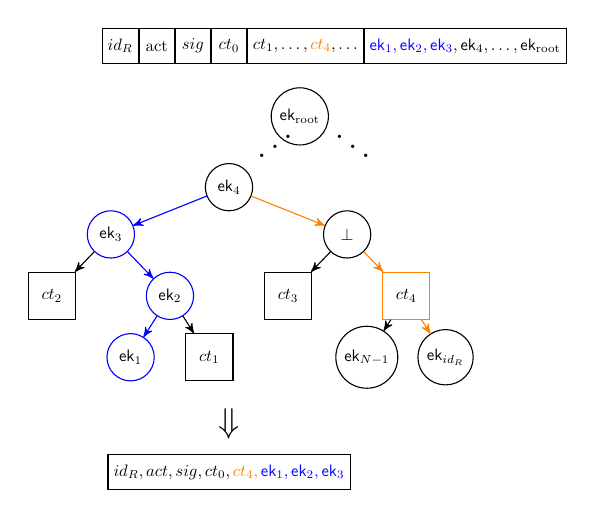
\begin{tikzpicture}[->,>=stealth',level/.style={sibling distance = 5cm/#1,
      level distance = 1.3cm},scale=0.6, transform shape,
    treenode/.style = {circle, draw=black, align=center, minimum size=1cm},
    ctnode/.style = {rectangle, draw=black, align=center, minimum size=1cm},
    packnode/.style = {rectangle, draw=black, align=center, minimum size=.75cm}]
    \tikzstyle{level 1}=[level distance=1cm]
    
    \node[packnode](pack){$id_R$};
    \node[packnode, right = 0cm of pack](pack2){act};
    \node[packnode, right = 0cm of pack2](pack3){$sig$};
    \node[packnode, right = 0cm of pack3](pack4){$ct_0$};
    \node[packnode, right = 0cm of pack4](pack5){$ct_1,\ldots, {\color{orange}ct_4}, \ldots$};
    \node[packnode, right = 0cm of pack5](pack6){${\color{blue}\mmpkepk_1,\mmpkepk_2,\mmpkepk_3},\mmpkepk_4, \ldots, \mmpkepk_{\text{root}}$};
    
    \node[below = 2.1cm of pack4, treenode](root){$\mmpkepk_4$}
    child[draw=blue]{
      node[treenode,draw=blue]{$\mmpkepk_3$}
      child[draw=black]{
        node[ctnode]{$ct_2$}
      }
      child[draw=blue]{
        node[treenode,draw=blue]{$\mmpkepk_{2}$}
        child{
          node[treenode,draw=blue]{$\mmpkepk_{1}$}
        }
        child[draw=black]{
          node[ctnode]{$ct_1$}
        }
      }
    }
    child[draw=orange]{
      node[treenode]{$\bot$}
      child[draw=black]{
        node[ctnode]{$ct_3$}
      }
      child{
        node[ctnode, draw=orange]{$ct_4$}
        child[draw=black]{
          node[treenode]{$\mmpkepk_{N-1}$}
        }
        child{
          node[treenode]{$\mmpkepk_{id_R}$}
        }
      }
    };
    \node[above right = .1cm of root](dots){\huge$\iddots$};
    \node[right = .6cm of dots]{\huge$\ddots$};
    \node[above right = 1cm of root, treenode]{$\mmpkepk_{\text{root}}$};
    \node at ($(root) + (0,-5)$)(arrow){\huge$\Downarrow$};
    \node[packnode, below = .2cm of arrow] {$id_R, act, sig, ct_0, \color{orange}{ct_4}, \color{blue}{\mmpkepk_1,\mmpkepk_2,\mmpkepk_3}$};
  \end{tikzpicture}  
  \caption{Server extraction algorithm. Lowest common ancestor (LCA) pof $id_R$ and $id_S$ is $\mmpkepk_4$, so all blue
    public keys are included in $id_R$'s packet. Since the sibling of $\mmpkepk_3$ is empty, there corresponding path
    secret of $\mmpkepk_4$ is encrypted to its resolution, resulting in the two ciphertext.
    % MM: Removed the part about c_0 since we din't use it in the main body
%    parts $ct_3$ and $ct_4$. $id_R$ can decrypt $ct_4$, since it lies on its path (orange) to the LCA . The signature and
%    header are included in every package, as well as the ciphertext-independent part ($ct_0$) of the \mmPKE encryption.
}
  \label{fig:extract-one}
\end{figure}

%%% Local Variables:
%%% mode: latex
%%% TeX-master: "main"
%%% End:


\paragraph{Comparison with techniques of \cite{hashimoto2021cmpke}.}
The work \cite{hashimoto2021cmpke} introduces a technique for efficient packet authentication which is quite similar to the technique used by \saik. In particular, their CGKA uses a committing mPKE, cmPKE. A cmPKE differs from mPKE in that encryption outputs a tag $T$ which is a cryptographic commitment to the plaintext and is delivered to each receiver. Since in \cite{hashimoto2021cmpke} every recipient of a commit gets the same message, authenticating $T$ is sufficient for CGKA authentication.
%
We highlight a couple of differences between that technique and ours:
First, it is not clear how to use cmPKE in a tree-based CGKA, where a commit executes multiple instances of \protCMPKE, and hence we end up with multiple tags $T$, each delivered to a different subset of the group.
%
Second, using the hash of the encrypted message as $T$ does not result in an IND-CCA secure \protCMPKE, since a hash allows to easily tell which of two messages is encrypted. Therefore, the construction of \cite{hashimoto2021cmpke} uses key-committing encryption to both hide and bind the message.

To summarize, \protCMPKE introduced by \cite{hashimoto2021cmpke} is very useful for the CGKA type they consider and may well find more use-cases beyond CGKA. On the other hand, \textsf{SAIK}’s solution fits all types o CGKA, does not require additional properties to prove CGKA security and is more direct. Albeit, it is very CGKA-specific.
%%% Local Variables:
%%% mode: latex
%%% TeX-master: "main"
%%% End:

% !TEX root = main.tex
% !TeX spellcheck = en_US

\section{Security of \saik}\label{sec:saik-sec-int}
To define the security we prove for \saik we fix the two safety
predicates \KwConf{} and \KwAuth{} used by $\funcCGKA$. We next give the intuition; see \cref{fig:safe} in \cref{sec:bgm_prot_proof} for the pseudocode. We define two versions of the
predicates: a stronger and a weaker one. For better exposition, the
stronger version is not achieved by \saik as presented in this work. But at the cost of added complexity
\saik can easily be extended to achieve it, as
described \cref{sec:ext-sec-predicates}.

We begin with the simpler stronger version. First, both predicates give no
guarantees for epochs in detached trees until they are attached and so we
ignore them in this section. Then, the definition is built around the notion of
secrets which make up the protocol state. There are two types of secrets:
group secrets, stored in the state of all parties, and individual secrets,
stored in the states of some parties. Each corruption exposes a number of
secrets and each epoch change replaces a number of secrets by (possibly)
secure ones. The helper predicate $\safeGrpSecsSecure{}(E)$ decides
if the group secrets in $E$ are secure, i.e., not exposed, and the
predicate $\safeIndSecsSecure(E, \id)$ decides if $\id$'s individual
secrets in $E$ are secure.
%
Then $\KwConf{}(E)$ equals to
$\safeGrpSecsSecure{}(E)$, since the epoch key is itself a group
secret. Further, $\KwAuth{}(E, \id)$ is true if either
$\safeGrpSecsSecure{}(E)$ or
$\safeIndSecsSecure(E,\id)$ is true, because both group and $\id$'s secrets
are necessary to impersonate $\id$ in $E$.

It remains to determine when group and individual secrets are exposed. For
group secrets, $\safeGrpSecsSecure(E)$ is defined recursively. The
base case states that the group secrets in first epoch (when the group was
created) are secure if and only if no party is corrupted while in that epoch.
Intuitively, we assume the group was created by an honest party using good
randomness. Moreover, capturing perfect forward secrecy, corruptions in the
descendant epochs do not affect the confidentiality of earlier group secrets.

The induction step states that the group secrets in a non-root epoch $E$
are secure if no party is corrupted in $E$, the epoch is not created
by an injected packet from the adversary and either the group secrets in
$E$'s parent $E_p$ are secure or all individual secrets in
$E$ are secure. Intuitively, this formalizes the requirement that the
adversary can learn the group secrets in only three ways: A) by corrupting a
party currently in epoch $E$. B) by injecting the secrets (though
most injections are disallowed by the authenticity predicate). C) by
computing them the same way an honest \emph{receiver} transitioning to
$E$ would. The latter requires knowing the group secrets of
$E_p$ and the individual secrets of at least one receiver. Note that
the possible receivers are those parties that are group members in
$E$ and that are not $E$'s creator (who transitions on
sending). Note also that the fact that even knowing an epoch creator's individual
secrets in $E_p$ we can treat them as secure in $E$ which captures
so called \emph{post compromise security} (aka. \emph{healing} or
\emph{backwards security}). Indeed, in \saik, part of creating a new epoch
requires refreshing all ones individual secrets.

Finally, individual secrets of $\id$ in $E$ are exposed whenever
there is some other epoch $E'$ where $\id$'s secrets are the same as
in $E$ and where $\id$ was corrupted or its secrets were injected on
its behalf. The secrets of $\id$ are the same in two epochs if no epoch between them replaces the secrets, i.e., is created by $\id$, removes
it or adds it.

\paragraph{Weaker guarantees.}
In the weaker version of the security predicates, individual secrets of $\id$
in $E$ are not secure in an additional scenario, formalized by
\safeWeakAdd. In this scenario, an $\id_s$ first honestly adds $\id$ and the
adversary $\Adv$ injects a message adding $\id$ to some other epoch. Finally,
$\id$ joins $\Adv$'s epoch and is corrupted before sending any message. We explain why \saik is insecure in this case and how it can be modified to be secure in
\cref{sec:ext-sec-predicates}.

\paragraph{Security.} 
For the \mmPKE scheme we assume a security property called \mmowrcca, defined in \cref{sec:mmowrcca}. The notion is strictly weaker than \mmindcca; in \cref{sec:mmowrcca} we prove the implication.
%
Formally, the AKS is modeled as the functionality $\funcPKI$ defined in \cref{sec:pki}. \saik
works in the $\funcPKI$-hybrids model, i.e., $\funcPKI$ is available in the real world and emulated by the simulator in the ideal world.

\newcommand{\ucideal}{\textnormal{\textsc{ideal}}}
\newcommand{\ucreal}{\textnormal{\textsc{real}}}
\begin{restatable}{theorem}{itkSec}\label{thm:saik-security}
	Let $\funcCGKA$ be the CGKA functionality with predicates \KwConf{} and \KwAuth{} defined in \cref{fig:safe}. Let $\saik$ be instantiated with an mmPKE \mmPKE, a signature scheme \sigscheme and \mac, and with the \hkdf functions modelled as a random oracle \hash.
	Let $\Adv$ be any environment. Denote the output of $\Adv$ from the real execution with \saik and the hybrid functionality $\funcPKI$ from \cref{fig:aks} as $\ucreal_{\saik, \funcPKI}(\Adv)$ and the output of $\Adv$ from the ideal execution with $\funcCGKA$ and a simulator $\ucsim$ as $\ucideal_{\funcCGKA, \ucsim}(\Adv)$.
	%
	There exists a simulator $\ucsim$ and adversaries $\Bdv[1]$ to $\Bdv[4]$ such that
	\begin{align*}
		\Pr[\ucideal&_{\funcCGKA, \ucsim}(\Adv) = 1] - \Pr\left[\ucreal_{\saik, \funcPKI}(\Adv) = 1\right] \leq \\
		&\textnormal{Adv}^{\gamefont{CR}}_{\hash}(\Bdv[1]) \\
		% confidentiality
		+\ & q_e^2(q_e+1) \log(q_n) \cdot\textnormal{Adv}^\mmowrcca_{\mmPKE,q_e\log(q_n),q_n}(\Bdv[2]) \\
		% authenticity asym
		+\ & 2q_e\cdot \textnormal{Adv}^{\ufcma}_\sigscheme(\Bdv[3]) \\
		+\ & q_e \cdot \textnormal{Adv}^{\ufcma}_\mac(\Bdv[4]) + 3q_hq_e^2(q_e+1)/2^\kappa,
	\end{align*}
	where $q_e$, $q_n$ and $q_h$ denote bounds on the number of epochs, the group size and the number of $\Adv$'s queries to the random oracle modelling the $\hash$, respectively.
	%  In the reductions, the $\hkdf$ functions are modelled as a random oracle.
  \end{restatable}

  The formal proof of \cref{thm:saik-security} can be found in \cref{sec:bgm_prot_proof}.

%%% Local Variables:
%%% mode: latex
%%% TeX-master: "main"
%%% End:

% !TEX root = main.tex
% !TeX spellcheck = en_US

\section{Evaluation}\label{sec:eval}
We compare the communication complexity or, informally, the ``bandwidth'' of \saik, \protITK and \protCMPKE from \cite{hashimoto2021cmpke}. For the sake of this comparison (and to simplify the description), one
can think of \protCMPKE as a protocol similar to \saik but where the ratchet tree is an $N$-ary tree of height $1$, where $N$ is the number of group members.
This means that \protCMPKE only needs single-message multi-recipient PKE, \mPKE (which is a special case of mmPKE).
To make a fair comparison, we instantiate \protCMPKE with the same DH-based \mPKE as \saik
instead of the less efficient but post-quantum secure \mPKE
given in \cite{hashimoto2021cmpke}.
%formulas in \cref{tab:bandwidth}.

\paragraph{Methodology.}
We compare the communication complexity of \emph{a single group modification} with respect to three metrics:
\begin{itemize}
	\item  \emph{sender bandwidth} -- the size of the packet uploaded to the
server,
\item  \emph{maximum receiver bandwidth} -- the maximum size of a (personalized) packet downloaded by a single
receiver, and
\item   \emph{total bandwidth} --  the sum of the sizes of the uploaded packet and all downloaded packets.
\end{itemize}
The sender and maximum-receiver bandwidths give an idea about the resources a single client needs to invest to perform
the group modification. In contrast, the total bandwidth gives the idea about the resources used by the server (or,
equivalently, all clients together). However, it makes no assertions about the distribution of this bandwidth, i.e. some
clients might use a significantly larger portion of the total bandwidth than others. (We note that the total bandwidth was the (only) metric used in \cite{hashimoto2021cmpke}.)

There is one caveat when calculating the bandwidth requirements for \saik (and \protITK) due to the underlying tree structure: The bandwidth can vary quite
significantly depending on the ``tree topology'', which is in turn determined by the execution history. Roughly, the reason is that add and remove operations may destroy the
good properties of the tree (by ``blanking'' nodes), increasing the number of public keys to which some message must be encrypted. In the
best case, called the \emph{tree-best-case}, there are only $\log(N)$ public keys (this happens when the ratchet has no blank nodes or unmerged
leaves, as depicted in \cref{fig:tree-full}). However, in the worst case, called the \emph{tree-worst-case}, there can be
$N$ public keys (this happens e.g. when all non-leaf nodes are blank; see \cref{fig:tree-blank}). In general, the number of public keys can be anything in between; see \cref{fig:tree-mixed}.

\begin{figure}[!tb]
  \centering
  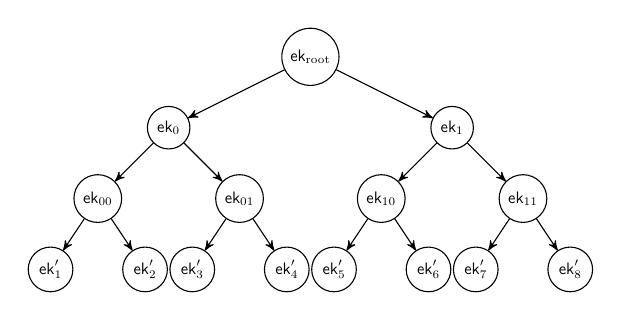
\begin{tikzpicture}[->,>=stealth',level/.style={sibling distance = 6cm/#1,
      level distance = 1.5cm},scale=0.6, transform shape,
    treenode/.style = {circle, draw=black, align=center, minimum size=.9cm}]
    
    \node[treenode](root){$\mmpkepk_{\text{root}}$}
    child{
      node[treenode]{$\mmpkepk_{0}$}
      child{
        node[treenode]{$\mmpkepk_{00}$}
        child{
          node[treenode]{$\mmpkepk'_{1}$}
        }
        child{
          node[treenode]{$\mmpkepk'_{2}$}
        }       
      }
      child{
        node[treenode]{$\mmpkepk_{01}$}
        child{
          node[treenode]{$\mmpkepk'_{3}$}
        }
        child{
          node[treenode]{$\mmpkepk'_{4}$}
        }
      }
    }
    child{
      node[treenode]{$\mmpkepk_{1}$}
      child{
        node[treenode]{$\mmpkepk_{10}$}
        child{
          node[treenode]{$\mmpkepk'_{5}$}
        }
        child{
          node[treenode]{$\mmpkepk'_{6}$}
        }       
      }
      child{
        node[treenode]{$\mmpkepk_{11}$}
        child{
          node[treenode]{$\mmpkepk'_{7}$}
        }
        child{
          node[treenode]{$\mmpkepk'_{8}$}
        }
      }
    };
  \end{tikzpicture}
  \caption{A ratchet tree for \saik or \protITK without blanks or unmerged leaves.}
  \label{fig:tree-full}
\end{figure}


\begin{figure}[!tb]
  \centering
    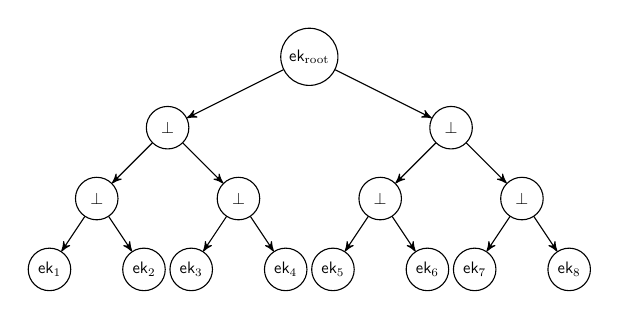
\begin{tikzpicture}[->,>=stealth',level/.style={sibling distance = 6cm/#1,
      level distance = 1.5cm},scale=0.6, transform shape,
    treenode/.style = {circle, draw=black, align=center, minimum size=.9cm}]

    \node[treenode](root){$\mmpkepk_{\text{root}}$}
    child{
      node[treenode]{$\bot$}
      child{
        node[treenode]{$\bot$}
        child{
          node[treenode]{$\mmpkepk_{1}$}
        }
        child{
          node[treenode]{$\mmpkepk_{2}$}
        }       
      }
      child{
        node[treenode]{$\bot$}
        child{
          node[treenode]{$\mmpkepk_{3}$}
        }
        child{
          node[treenode]{$\mmpkepk_{4}$}
        }
      }
    }
    child{
      node[treenode]{$\bot$}
      child{
        node[treenode]{$\bot$}
        child{
          node[treenode]{$\mmpkepk_{5}$}
        }
        child{
          node[treenode]{$\mmpkepk_{6}$}
        }       
      }
      child{
        node[treenode]{$\bot$}
        child{
          node[treenode]{$\mmpkepk_{7}$}
        }
        child{
          node[treenode]{$\mmpkepk_{8}$}
        }
      }
    };
  \end{tikzpicture}
  \caption{A ratchet tree for \saik or \protITK with all nodes blank.}
  \label{fig:tree-blank}
\end{figure}


\begin{figure}[!tb]
  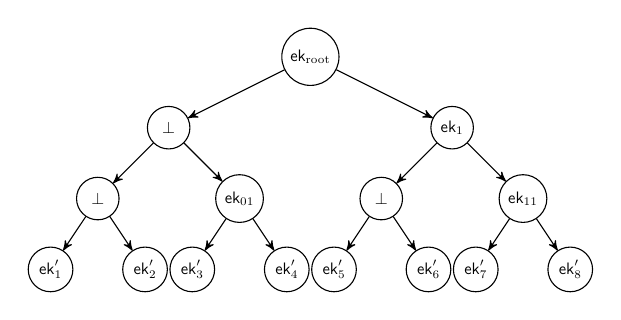
\begin{tikzpicture}[->,>=stealth',level/.style={sibling distance = 6cm/#1,
      level distance = 1.5cm},scale=0.6, transform shape,
    treenode/.style = {circle, draw=black, align=center, minimum size=.9cm}]
    
    \node[treenode](root){$\mmpkepk_{\text{root}}$}
    child{
      node[treenode]{$\bot$}
      child{
        node[treenode]{$\bot$}
        child{
          node[treenode]{$\mmpkepk'_{1}$}
        }
        child{
          node[treenode]{$\mmpkepk'_{2}$}
        }       
      }
      child{
        node[treenode]{$\mmpkepk_{01}$}
        child{
          node[treenode]{$\mmpkepk'_{3}$}
        }
        child{
          node[treenode]{$\mmpkepk'_{4}$}
        }
      }
    }
    child{
      node[treenode]{$\mmpkepk_{1}$}
      child{
        node[treenode]{$\bot$}
        child{
          node[treenode]{$\mmpkepk'_{5}$}
        }
        child{
          node[treenode]{$\mmpkepk'_{6}$}
        }       
      }
      child{
        node[treenode]{$\mmpkepk_{11}$}
        child{
          node[treenode]{$\mmpkepk'_{7}$}
        }
        child{
          node[treenode]{$\mmpkepk'_{8}$}
        }
      }
    };
  \end{tikzpicture}
  \caption{A tree with some blank and non-blank nodes. Here, sender bandwidth depends on the position in the
    tree. For example, a packet by the leftmost leaf would contain 5 ciphertexts, while the rightmost leaf would require 6.}
  \label{fig:tree-mixed}
\end{figure}

%%% Local Variables:
%%% mode: latex
%%% TeX-master: "main"
%%% End:


Therefore, we compare each bandwidth in the tree-best-case and the tree-worst-case. Note that any other case results in a bandwidth between these cases.
We remark that comparing the average over all histories of group operations would not be meaningful, since the probability of a given execution depends on user and administrator behavior, general application policies and runtime conditions, etc.
It is an important topic of future research to
better understand which kinds of policies governing when and which parties
initiate CGKA operations lead to more bandwidth efficient executions for
realistic deployments. However, it is outside the scope of this work.
%
We note that SAIK is \emph{very} flexible as to kinds of policies that are possible and the types of data that can be leveraged to guide executions towards efficient behavior. Thus, we conjecture that in practice a well designed implementation (of both server and client) will be able to ensure that under relatively mild real-time conditions the vast majority of executions will spend the overwhelming majority of their time tending towards the tree-best-case scenario in bandwidth.


\newcommand{\ctxSize}{\variable{Ctx}}
\newcommand{\mCtxSize}{\variable{mCtx}}
\newcommand{\pkSize}{\variable{Pk}}
\begin{figure*}[!p]
	\begin{minipage}[t]{\textwidth}\centering
	\begin{tabular}{|l|l|l|l|l|}
		\hline
		\multicolumn{2}{|c|}{}& \protITK & \saik & \protCMPKE \\
		\hline
		\multirow{2}{*}{Sender} 
		& tree-best-case & $\log(N)\cdot (\pkSize + \ctxSize)$ & $\log(N) \cdot \pkSize + \mCtxSize(\log(N))$ & $\pkSize + \mCtxSize(N)$ \\\cline{2-5}
		& tree-worst-case & $\log(N)\cdot\pkSize + N\cdot \ctxSize$ & $\log(N) \cdot \pkSize + \mCtxSize(N)$ & $\pkSize + \mCtxSize(N)$ \\\hline
		Maximum
		& tree-best-case & $\log(N)\cdot (\pkSize + \ctxSize)$  & $\log(N) \cdot \pkSize + \ctxSize$  & $\pkSize + \ctxSize$ \\\cline{2-5}
		receiver & tree-worst-case &  $\log(N)\cdot\pkSize + N\cdot \ctxSize$ & $\log(N) \cdot \pkSize + \ctxSize$  & $\pkSize + \ctxSize$ \\
		\hline
		\multirow{2}{*}{Total} 
		& tree-best-case & $N\log(N)\cdot (\pkSize + \ctxSize)$  & $N\log(N) \cdot \pkSize + N\cdot\ctxSize + \mCtxSize(\log(N))$   & $N\cdot(\pkSize + \ctxSize) + \mCtxSize(N)$ \\\cline{2-5}
		& tree-worst-case &  $N(\log(N)\cdot\pkSize + N\cdot \ctxSize)$ & $N\log(N) \cdot \pkSize + N\cdot\ctxSize + \mCtxSize(N)$  & $N\cdot(\pkSize + \ctxSize) + \mCtxSize(N)$ \\
		\hline
	\end{tabular}
	\caption{Sender, receiver and total bandwidth for a group of size $N$ expressed as the number of ciphertexts and public keys included in the packet (apart from this, packets include only a constant-size header).
		$\pkSize$ denotes the size of a public key (the same for PKE and mmPKE). $\mCtxSize(X)$ denotes the size of an mmPKE multi-recipient ciphertext with overall number of receivers $X$. Note that for the DH-based construction $X$ fully determines the size (i.e., it is not affected by who gets which message). $\ctxSize$ denotes the size of a PKE ciphertext, equal to the size of an individual ciphertext in the DH-based construction.
	}
	\label{tab:bandwidth1}
\end{minipage}
  \begin{minipage}[t]{.48\textwidth}
	\begin{minipage}[t]{\linewidth}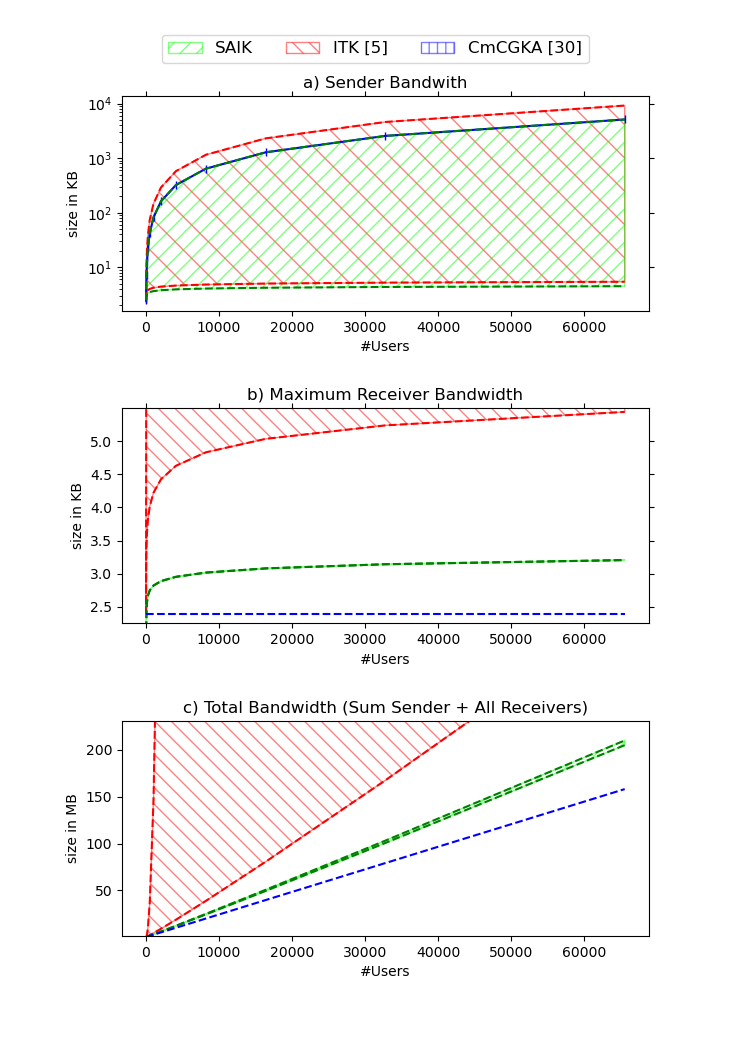
\includegraphics[width=\linewidth]{Final_Figures_Total}\end{minipage}
	\caption{Bandwidth comparison of \saik, \protITK and \protCMPKE (instantiated with 256-bit
		security). Lower lines denote the tree-best-case execution history, while upper lines denote the
		tree-worst-case. All other possible cases are marked as the regions between the lines. Plot (a) shows the sender
        bandwidth on a \emph{log scale} and plot 
		(b) shows average individual receiver bandwidth on a \emph{linear scale}. Plot (c) shows the total bandwidth,
        i.e. the sum of sender bandwidth and $n$ times the receiver bandwidth. Note that in the first plot, the lines for tree-worst-case \saik and
		all-case \protCMPKE coincide.
		%Sender and receiver bandwidth for a group of size $N$ expressed as the (approximate) number of group elements.
	}
	\label{tab:plots}
  \end{minipage}
  \hfill
  \begin{minipage}[t]{.48\textwidth}
    \centering\vspace*{-9.5cm}
    \begin{minipage}[t]{\linewidth}
    	\begin{tabular}{|l|l|l|l|l|}
    		\hline
    		\multicolumn{2}{|c|}{}& \protITK & \saik & \protCMPKE \\
    		\hline
    		\multirow{2}{*}{Sender} 
    		& best case & $3\log(N)$ & $2\log(N)$ & $N$ \\\cline{2-5}
    		& worst case &$2N$ & $N$ & $N$ \\\hline
    		\multirow{2}{*}{\parbox{1.5cm}{(Maximum)\\receiver}} 
    		& best case & $3\log(N)$ & $\log(N)$&  $3$ \\\cline{2-5}
    		& worst case & $2N$ & $\log(N)$ & $3$ \\ \hline
            \multirow{2}{*}{Total}
            & best case & $3N\log(N)$ & $N\log(N)$ & $4N $ \\\cline{2-5}
            & worst case & $2N^2$ & $N\log(N)$ & $4N$ \\
    		\hline
    	\end{tabular}
    \caption{
    	Sender, receiver and total bandwidth for a group of size $N$ expressed as the (approximate) number of group
        elements. Best/Worst case refers to the state of the tree, while we always consider the average receiver
        bandwidth over all receivers.
    }\label{fig:bandwidth2}
  \end{minipage}


  \begin{minipage}[t]{\linewidth}\centering
    \begin{tabular}{|l|r|}
      \hline
      & Bitsize \\
      \hline
      Group element & 512 \\
      \hline
      Hash & 512 \\
      \hline
      Signature & 1024 \\
      \hline
      Header & 17784 \\
      \hline
      \pkSize & 512 \\
      \hline
      \ctxSize & 1152 \\
      \hline
      $\mCtxSize(N)$ & $512 + N \cdot 640$ \\
      \hline
    \end{tabular}
    \caption{Bitsizes used to generate \cref{tab:plots}. The header consists of the sender's id, the epoch id and some
      authenticated data required by the protocol. The individual ciphertexts consist of a group element and an AEAD
      encryption, while the \mPKE ciphertext all share the same group element. The header contains signatures, tags,
      epoch and sender identifier as well as a key package. The latter makes up the bulk of the header, as it contains
      credentials, more public keys and some application data. Our estimation is based on MLS.}
    \label{tab:bits}
  \end{minipage}
  \end{minipage}
\end{figure*}
\paragraph{Results.}
We estimated the bandwidth for all protocols using the formulas in \cref{tab:bandwidth1,fig:bandwidth2} with bit lengths
indicated in \cref{tab:bits}. This is further visualized in \cref{tab:plots} for growing group sizes $N$.
We highlight some interesting observations. % features of the plots. %For concreteness, we fix $N = 10K$ users.

In terms of the sender bandwidth, \saik is always at least as good as the other protocols. 
For example, in a group of 10K parties, \saik sender's require between $83\%$ and $55\%$ of the bandwidth of \protITK (due to the smaller mmPKE ciphertexts compared to PKE). \saik's tree-worst-case sender bandwidth is the same as \protCMPKE but its tree-best-case bandwidth can be as small as $0.52\%$ by using only $4$KB in stead of \protCMPKE's $783$KB. (Recall that, unlike in \protCMPKE, in \saik sender bandwidth varies depending on the history of preceding operations.)


In terms of the maximum receiver bandwidth, \protITK is much worse than \saik and \protCMPKE. For
example, \saik receivers (at most) need between $62\%$ (tree-best-case execution) to about $.2\%$ (tree-worst-case
execution) of \protITK's. On the other hand, \protCMPKE is the best for receivers.  \saik requires up
to $126\%$ of \protCMPKE's bandwidth, i.e. an increase from $\sim 2.4$KB to $\sim 3.02$KB for 10K parties.

Finally, the total bandwidth is by far the smallest for \protCMPKE and by far the largest for \protITK. For instance,
for 10K parties, \saik requires $\sim1.3$ times more total bandwidth, while \protITK requires anywhere from $\sim2$
times (tree-best-case) to $\sim50$ times (tree-worse-case) more.

In summary, the results show that \saik achieves the lowest bandwidth required from a single client
(i.e. $\bigO(\log(N))$ for \saik vs. $\bigO(N)$ for \protCMPKE), while \protCMPKE has the lowest total bandwidth
(i.e. $\bigO(N\log(N))$ for \saik vs. $\bigO(N)$ for \protCMPKE). (Hence, both protocols meet their design goals.) For instance, for 10K parties, \protCMPKE requires a client to upload $783$KB of data, while in scenarios close to the tree-best-case (which we believe to occur most of the time), the sender or receiver bandwidth of \saik is roughly $4$KB. On the other hand, the total bandwidth is roughly $25$MB for \protCMPKE and $30$MB for \saik.

\paragraph{Server computation.}
Lastly, we consider the server-side computation for \saik and \protCMPKE. In \protCMPKE, the server only picks the
$i$-th \mPKE ciphertext for the $i$-th user and forwards all common data. For \saik, we can consider two possibilities:
Either the server keeps track of the shape of the ratchet tree (which it can do based on the header data sent in all
packages) and computes the lowest common ancestor of sender and receiver in the tree, computes its resolution and then
forwards the corresponding ciphertext and public keys. This takes at most logarithmic time in the size of the
group (however, no expensive public-key operations are required). Alternatively, the user can compute its indices in the
tree and send them to the server, reducing the server computation to effectively the same as in \protCMPKE at the cost
of an additional round of communication.

%%% Local Variables:
%%% mode: latex
%%% TeX-master: "main"
%%% End:

% !TEX root = main.tex
% !TeX spellcheck = en_US

\section{Extensions}\label{sec:extensions}
In this section we describe extensions of \saik which we did not include for simplicity.% The first extension allows to achieve slightly better security predicates at a relatively small cost. The second extension deals with primitives with imperfect correctness, such as mmPKE based on lattices.

% \subsection{Trading-off Server Computation for Communication}
% Our new (sa)CGKA \saik assumes that the mailboxing service is a full featured server capable of performing the
% individualization of messages responsible for the improved bandwidth of our protocol. This individualization mainly
% consists of generating proofs of accumulation. We assume strong accumulators which allow creation of these proofs
% without secret knowledge. However, we can trade off this server computation for increased sender communication by having the
% sender pre-compute all proofs and send them along with the rest of the packet. Receiver communication is unaffected
% by this change.

% For the hash-based accumulator described in \cref{sec:accumulators}, an easy optimization is possible. Instead of
% computing \emph{all} proofs individually, the sender can instead include the whole Huffman tree in its package. The
% server then only selects the co-paths in the tree relevant for each user, which is similarly complex to selecting the
% correct message for each user, which is exactly the task of a standard mailboxing service. This approach increases
% communication by approximately $2N$ hashes, where $N$ is the number of receiving public keys, i.e. linear in the
% number of group members in the worst case and logarithmic in the best case.

% In conclusion, our saCGKA can be transformed into a regular CGKA at the cost of sender communication while avoiding
% server computation.

% Note that the variant where each submessage is signed individually requires less communication (i.e. $N$ signatures
% instead of $2N$ hashes) than the transformed \saik variant and also doesn't require server computation. However,
% computing each signature requires an expensive public key operation, leading to a shorter sender message, but more computation for the
% sender than required by the server in \saik.

\subsection{Better Security Predicates}\label{sec:ext-sec-predicates}
We sketch the reason why \saik does not achieve the better security predicates and how it can be modified to achieve them.

Roughly, \saik achieves the worse security predicates because of the following attack: Say $\id_s$, the only corrupted party, creates a new epoch $E$ adding a new member $\id$. According to \saik, in this case $\id_s$ fetches from the Authenticated Key Service, AKS, (a type of PKI setup) a public key $\mmpkepk$ for \mmPKE and a verification key $\spk$ for \sigscheme, both registered earlier by $\id$. In epochs after $E$, parties use $\mmpkepk$ to encrypt messages to $\id$ (even before $\id$ actually joins) and $\spk$ to verify messages from $\id$. Now the adversary $\Adv$ can create a fake epoch $E'$ adding $\id$ with the same $\mmpkepk$ and $\spk$. Then, $\id$ joins $E'$ and is corrupted, leaking $\mmpkesk$ and $\ssk$. This allows $\Adv$ to compute the group key in $E$ and inject messages to parties in $E$. However, the expectation is that this is not possible, since no party is corrupted in $E$ (and $\id_s$ healed).
%
The better security predicates (formally, the predicates in \cref{fig:safe} in \cref{sec:bgm_prot_proof}) achieve just this: security in an honest epoch $E$ does not depend on whether some member joins a fake group in $E'$.

The following modification to \saik achieves better security: We note that in \saik, $\id$ registers in the AKS an additional public key $\mmpkepk'$ which is used to send secrets needed for joining. The corresponding $\mmpkesk'$ is deleted immediately after joining. In the modified \saik, when $\id_s$ adds $\id$, it generates for $\id$ new key pairs $(\mmpkepk_s,\mmpkesk_s)$ and $(\spk_s,\ssk_s)$. It sends $\mmpkesk_s$ and $\ssk_s$ to $\id$, encrypted under $\mmpkepk'$. Now messages to $\id$ are encrypted such that \emph{both} $\mmpkesk$ and $\mmpkesk_s$ are needed to decrypt them. In particular, to encrypt $m$, a sender chooses a random $r$ and encrypts $r$ under $\mmpkepk$ and $m \oplus r$ under $\mmpkepk_s$. Similarly, messages from $\id$ have two signatures, one verified under $\spk$, and one under $\spk_s$. As soon as $\id$ creates an epoch, it generates a new single \mmPKE key pair and a single \ers key pair.

The attack is prevented, because even after corrupting $\id$ in $E'$, $\Adv$ does not know $\mmpkesk'$ needed to decrypt $\mmpkesk_s$ and $\ssk_s$. Therefore, confidentiality and authenticity in $E$ is not affected.

\subsection{Primitives with Imperfect Correctness}
While the proofs of \saik security assume primitives with perfect correctness, they can be easily modified to work with
imperfect correctness. While most classically secure primitives have perfect correctness, many post-quantum
constructions (e.g. from lattices) only have statistical correctness. So this extension can be seen as a preparation for
when \saik has to be adapted to post-quantum security.

This is achieved by adding one game hop where we
abort in the new game if a correctness error occurs. This loses an additive term in the security bound that depends on
the correctness parameter and the number of possible occurrences. Additionally, the usage of primitives with imperfect
correctness generally yields imperfect correctness guarantees for the application as well (potentially with
multiplicative correctness error when using multiple primitives). For completeness, we give definitions of imperfect
correctness of the primitives used directly by \saik in this section.

\begin{definition}
We call an \mmPKE scheme \emph{$\delta$-correct}, if for all $n\in \N$, $(\mmpkepk_i,\mmpkesk_i)\in
  \mmpkeKeyGen $ for $i\in[n]$,
  $(m_1,\ldots, m_n)\in\mathcal{M}^n$ and $\forall j\in[n]$
  \[
    \Pr\left[
      \begin{array}{c}
        c_j\gets \mmpkeExt(j, C)\\
        m_j \neq \mmpkeDec(\mmpkesk_j, c_j)
      \end{array}
      \middle\vert
      C \getsr \mmpkeEnc\left(
      \begin{array}{c}
        (\mmpkepk_1,\ldots, \mmpkepk_n),\\(m_1,\ldots,m_n)
      \end{array}
      \right)
    \right] \leq \delta
  \]
\end{definition}

% \begin{definition}
%   An HRS scheme \ers for a collection of reduction pattern classes $\rdclassset_n$ for $n\in\N$ is $\delta$-correct if for all $n \in \N$, $\rdclass \in \rdclassset_n$, $(\rd,w) \in \rdclass$ and message vectors $\vec m$ of length $n$, we have
%   \begin{equation*}
%     \Pr\left[\ersvrfy\left(
%     \begin{array}{c}
%       \ersvk, k, \rd(\vec{m}),\\ \rd, \sigma'
%     \end{array}
%     \right) \neq 1
%     \middle\vert
%     \begin{array}{c}
%       (\erssk, \ersvk) \gets \erskeygen()\\
%       k \getsr \bits^\kappa\\
%       \sigma \gets \erssign(\erssk, k, \vec{m}, \rdclass) \\
%       \sigma' \gets \ersred(\ersvk, \sigma, \vec{m},\rd)
%     \end{array}
%     \right] \leq \delta.
%   \end{equation*}
% \end{definition}

% Below, we also define $\delta$-correct weighted accumulator. It is easy to see that our construction of \ers instantiated with a $\delta$-correct accumulator is also $\delta$-correct.

% \begin{definition}
%   A weighted accumulator scheme $\wacc$ is \emph{$\delta$-correct} if for every set $X$ of element-weight pairs $(x,w)$ and each $x$ s.t. $(x,\wc)\in X$, we have
%   \[
%   \Pr
%   \left[
%   \accVrfy(\accValue, x, \accProof) \neq 1
%   \middle\vert
%   \begin{array}{c}
%     (\accValue, \accaux) \getsr \accEval(X) \\
%     \accProof \getsr \accProve(\accValue, x, \accaux)
%   \end{array}
%   \right]\leq \delta.
%   \]
% \end{definition}



%%% Local Variables:
%%% mode: latex
%%% TeX-master: "main"
%%% End:


%--- Bibliography --------------------------------------------------------------
%\bibliographystyle{plain} %if need be use {plain}
%%\bibliographystyle{splncs04}
%\bibliography{project,../cryptobib/abbrev3,../cryptobib/crypto}
\bibliographystyle{ACM-Reference-Format}
\bibliography{project,../cryptobib/abbrev3,../cryptobib/crypto}


%--- Appendix ------------------------------------------------------------------
\clearpage
\newpage
\appendix

\begin{center}\Huge
	Supplementary Material
\end{center}

\section{Additional Preliminaries} \label{sec:addPrelim}

\subsection{Universal Composability}\label{sec:uc}
We formalize security in the universal composability (UC) framework \cite{FOCS:Canetti01}. We moreover use the modification of responsive environments introduced by Camenisch et
al.~\cite{AC:CEKKR16} to avoid artifacts arising from seemingly local operations (such as sampling randomness or
producing a ciphertext) to involve the adversary.

The UC framework requires a real-world execution of the protocol to be indistinguishable from an ideal world, to an an interactive environment.
%
The real-world experiment consists of the group members executing the protocol (and interacting with the PKI setup).
In the ideal world, on the other hand, the protocol gets replaced by dummy instances that just forward all inputs and outputs to
an \emph{ideal functionality} characterizing the appropriate guarantees.

The functionality interacts with a so-called simulator, that translates the real-world adversary's actions into corresponding ones in the ideal world. Since the ideal functionality is secure by definition, this implies that the real-world execution cannot exhibit any attacks either.


\paragraph{The Corruption Model.}
We use the --- standard for CGKA/SGM but non-standard for UC --- corruption model of continuous state leakage (transient passive corruptions) \cite{TCC:ACJM20}.\footnote{Passive
  corruptions together with full network control allow to emulate active corruptions.}
%
In a nutshell, this corruption model allows the adversary to
repeatedly corrupt parties by sending corruption messages of the form $(\keyword{Expose}, \id)$, which causes the party $\id$ to send its current state to the adversary (once).

\paragraph{Restricted Environments.}
In order to avoid the so-called commitment problem, caused by adaptive corruptions in simulation-based frameworks, we restrict the environment not to corrupt parties at certain times. (This roughly corresponds to ruling out ``trivial attacks'' in game-based definitions. In simulation-based frameworks, such attacks are no longer trivial, but security against them requires strong cryptographic tools and is not achieved by most protocols.)
%In order to avoid the so-called commitment problem\footnote{The commitment problem causes standard UC definitions to be extremely strong in the presence of adaptive corruptions, ruling out any practical protocols such as \mls.}
%of simulation-based security notions such as UC, we restrict the environment not to corrupt parties at certain times. (This roughly corresponds to ruling out ``trivial wins'' in game-based definitions.)
%
To this end, we use the technique used in \cite{TCC:ACJM20} (based on prior work by Backes et al.~\cite{ESORICS:BDDK06} and Jost et al.~\cite{TCC:JosMauMul19}) and consider a weakened variant of UC security that only quantifies over a restricted set of so-called admissible environments that do not exhibit the commitment problem.
%
%Whether an environment is admissible or not is defined by the ideal functionality $\Func$ with statements of the form $\KwRestrEnv\ \mathit{cond}$ and an environment is called {admissible (for $\Func$)}, if it has negligible probability of violating any such $\mathit{cond}$ when interacting with $\Func$.
Whether an environment is admissible or not is defined as part of the ideal functionality $\Func$: The functionality can specify certain boolean conditions, and an environment is then called {admissible (for $\Func$)}, if it has negligible probability of violating any such condition when interacting with $\Func$.

% \subsection{Collision-Resistant Hashing}
% We define collision resistance for hash functions in \cref{def:cr}.
% \begin{definition}[Collision Resistance]\label{def:cr}
%   Let $\hash:\bits^* \rightarrow \bits^\kappa$ be a hash function. We define the advantage of an adversary \Adv against
%   the collision resistance of $\hash$ as
%   \[
%     \adv{\CR}{\hash}(\Adv) = \Pr\left[\hash(x_1) = \hash(x_2)\mid (x_1,x_2)\getsr\Adv\right].
%   \]
% \end{definition}

% Note that for simplicity, we define \emph{unkeyed} hash functions. Generally, these hash functions aren't collision
% resistant, since there always exists some algorithm that has a hard-coded collision. However since such algorithms are
% \emph{unknown} for real-world hash functions and we give constructive reductions (i.e. fully black-box reductions where
% access to an algorithm breaking our building blocks directly yields an algorithm finding a collision), we ignore these
% existing but unknown algorithms. For a more in-depth discussion, see \cite{VIETCRYPT:Rogaway06}.

\subsection{Assumptions}
The security of our mmPKE construction, same as that of \cite{ASIACCS:PinPoeSch14}, is based on a variant of the Computational
Diffie-Hellman(CDH) assumption called the \emph{Double-Sided Strong Diffie-Hellman Assumption} (or just \emph{Static
  Diffie-Hellman Assumption} in \cite{ASIACCS:PinPoeSch14}). We recall it in Definition~\ref{def:SDH}. Intuitively, it states that
CDH is hard given access to a DDH-oracle for both CDH inputs.

\begin{definition}[Double-Sided Strong Diffie-Hellman Assumption]\label{def:SDH}
  Let $\Group = (\Grp, p, g)$ be a cyclic group of prime order $p$ with generator $g$. We define the advantage of an
  algorithm $\Adv$ in solving the \emph{Double-Sided Strong Diffie-Hellman problem(\sdh)} with respect to $\Group$ as
  \[
    \adv{\sdh}{\Group}(\Adv) =
    \left[
      Z = g^{xy}
      \middle\vert
      \begin{array}{c}
        x, y \getsr \Z_p^2\\
        Z \getsr \Adv^{\oracle{O}}(\Grp,p,g,g^x,g^y),
      \end{array}
    \right]
  \]
with $\oracle{O} = \{\oracle{O}_x(\cdot,\cdot),\oracle{O}_y(\cdot,\cdot)\}$, where $\oracle{O}_x,\oracle{O}_y$ are oracles which on input $U,V$ output $1$, iff $U^x = V$ or $U^y = V$ respectively.
The probability is taken over the random coins of the group generator, the choice of $x$ and $y$ and the adversary's
random coins.
\end{definition}

\subsection{Multi-Recipient Multi-Message PKE(mmPKE) Definitions}\label{app:mmpke}
The notion of \mmindrcca security for \mmPKE is described by the experiment in \cref{fig:mmpke_rcca}.

\begin{figure}[!tbp]
  \begin{gamebox}{\mmindrcca}
    \begin{minipage}[t]{\linewidth}
      \algoHead{$\text{Exp}^{\mmindrcca}_{\mmPKE, \nUsers, b}(\Adv = (\Adv[1], \Adv[2]))$}
      \begin{algorithmic}
        \For{$\idxUser\in[\nUsers]$}
           $(\mmpkepk_\idxUser, \mmpkesk_\idxUser)\gets \mmpkeKeyGen()$
        \EndFor
        \State $\term{Corr} \gets \emptyset$
        \State \mbox{$(\vec\mmpkepk^*,\vec m_0^*,\vec m_1^*,\mathit{st}) \gets \Adv[1]^{\oracle{Dec}_1, \oracle{Cor}}((\mmpkepk_i)_{i\in[\nUsers]})$}

        \State \KwReq{} $\abs{\vec m_0^*}=\abs{\vec m_1^*}=\abs{\vec\mmpkepk^*}$
        \State $c^* \getsr \mmpkeEnc(\vec\mmpkepk^*,\vec{m}_b^*)$

        \State $b' \gets \Adv[2]^{\oracle{Dec}_2, \oracle{Cor}}(c^*,\mathit{st})$
        \State \KwReq{} $\leak(\vec{m_0}) = \leak(\vec{m_1})$
        \State \KwReq{} $\forall j : \vec \mmpkepk^*[j] \in \{\mmpkepk_i : i\in[\nUsers]\} \setminus \term{Corr} \lor m_0^*[j]=m_1^*[j]$
        \State \Return $b'$
      \end{algorithmic}
    \end{minipage}

  \medskip
    \begin{minipage}[t]{.4\linewidth}
      \algoHead{Oracle $\oracle{Dec}_1(i,c)$}
      \begin{algorithmic}
        \State \KwReq{} $\idxUser\in[\nUsers]$
        \State \Return $\mmpkeDec(\vec\mmpkesk[i],c)$
      \end{algorithmic}

      \medskip
      \algoHead{Oracle $\oracle{Cor}(\idxUser)$}
      \begin{algorithmic}
        \State \KwReq{} $\idxUser\in[\nUsers]$
        \State $\term{Corr} \setadd \idxUser$
        \State \Return $\mmpkesk_\idxUser$
      \end{algorithmic}
    \end{minipage}\hfill\begin{minipage}[t]{.59\linewidth}
      \algoHead{Oracle $\oracle{Dec}_2(i,c)$}
      \begin{algorithmic}
        \State \KwReq{} $\idxUser\in[\nUsers]$
        \State $m \gets \mmpkeDec(\vec\mmpkesk[i],c)$
        \If{$\exists j : \vec\mmpkepk^*[j] = \mmpkepk_i $ \\\strut\hfill $\land\ m \in \{\vec m_0^*[j], \vec m_1^*[j]\}$}
        \State \Return $\literal{test}$
        \Else\
        \Return $m$
        \EndIf
      \end{algorithmic}
    \end{minipage}
  \end{gamebox}
  \caption{\mmindrcca security game for \mmPKE with leakage function  $\leak(\vec m) = (\len(\vec m[1]), \dots, \len(\vec m[n]))$.}
  \label{fig:mmpke_rcca}
\end{figure}

We define the security of an \mmPKE in a left-right style in the following \cref{def:mmindrcca}.

\begin{definition}[\mmindrcca]\label{def:mmindrcca}
Let $N\in\N$. For a scheme \mmPKE, we define the advantage of an adversary \Adv against \emph{Indistinguishability Against Replayable Chosen Ciphertext Attacks (\mmindrcca)} security of \mmPKE as
\begin{multline*}
  \adv{\mmindrcca}{\mmPKE, \nUsers}(\Adv) = \Pr\left[\Exp^{\mmindrcca}_{\mmPKE,\nUsers, 0}(\Adv) = 1\right] \\ -
      \Pr\left[\Exp^{\mmindrcca}_{\mmPKE,\nUsers,1}(\Adv) = 1\right],
\end{multline*}
where $\textnormal{Exp}^{\mmindrcca}_{\mmPKE,N,b}$ is described in \cref{fig:mmpke_rcca}.
\end{definition}


\subsection{Data Encapsulation Meachanism(DEM)}
A DEM is the symmetric equivalent of a PKE scheme. We recall it in \cref{def:dem}.

\begin{definition}[DEM]\label{def:dem}
  A data encapsulation mechanism (DEM) \dem is described by a (efficiently samplable) keyspace $\demKeyset$ and the two
  algorithms $\demEnc, \demDec$:
  \begin{itemize}[align=left]
    \item[$\demEnc(k, m)\getsl c$:] The encryption algorithm takes a key $k\in\demKeyset$ and a message $m$. It returns a ciphertext $c$.
    \item[$\demDec(k, c) \getsl m'\lor\bot$:] The decryption algorithm takes a key $k\in\demKeyset$ and a
      ciphertext $c$ and outputs either a decrypted message or $\bot$.
    \end{itemize}
    A DEM \dem is $\delta$-correct, if for all messages $m$ and all keys $k\in\demKeyset$
    \[
      \text{Pr}[\demDec(k, \demEnc(k,m)) = m] \geq \delta
    \]
  \end{definition}

  Analogue to mmPKE, we consider \indrcca security for DEMs. It is described in \cref{def:dem_rcca}.

  \begin{definition}\label{def:dem_rcca}
    The advantage of an adversary \Adv against the \indrcca security of a DEM \dem is defined as
    \begin{multline*}
      \adv{\indrcca}{\dem}(\Adv) = \text{Pr}[\experiment{\indrcca}{\dem, 0}(\Adv) = 1] \\-
      \text{Pr}[\experiment{\indrcca}{\dem, 1}(\Adv) = 1],
    \end{multline*}
    where $\experiment{\indrcca}{\dem, b}(\Adv)$ is defined in \cref{fig:dem_rcca}.
  \end{definition}

  \begin{figure}[!tbh]
    \begin{gamebox}{\indrcca for \dem}
      \begin{minipage}[t]{.5\linewidth}
        \algoHead{Exp$^{\indrcca}_{\dem, b}(\Adv)$}
        \begin{algorithmic}
          \State $k\getsr \demKeyset$
          \State $(St, m_0^*, m_1^*) \getsr \Adv^{\text{Dec},\text{Enc}}$
          \State $c^* \getsr \demEnc(k, m_b)$
          \State \Return $\Adv^{\text{Dec},\text{Enc}}(St, c^*)$
        \end{algorithmic}
      \end{minipage}
    \hfill
      \begin{minipage}[t]{.48\linewidth}
        \algoHead{Oracle Dec$(c)$}
        \begin{algorithmic}
          \State $m' \getsr \demDec(k, c)$
          \If{$m' \in \{m_0^*, m_1^*\}$}
          \State \Return \keyword{test}
          \Else
          \State \Return $m'$
          \EndIf
        \end{algorithmic}
        \medskip
        \algoHead{Oracle Enc$(m)$}
        \begin{algorithmic}
          \State \Return $\demEnc(k, m)$
        \end{algorithmic}
      \end{minipage}
    \end{gamebox}
    \caption{\indrcca security for DEMs.}
    \label{fig:dem_rcca}
  \end{figure}

\subsection{Message Authentication Codes (MAC)}
Message authentication codes are defined in \cref{def:mac}.

\begin{definition}\label{def:mac}
  A message authentication code $\mac = (\mactag,$ $ \macvrf)$ consist of a keyspace $\mackeyspace$ and the following two
  algorithms:
  \begin{itemize}[align=left]
    \item[$\mactag(k, m)\getsl \mtag$:] The tagging algorithm takes a key $k$ and a message $m$ and outputs
      a tag $t$.
    \item[$\macvrf(k, m, \mtag)\getsl\bits$:] The verification algorithm takes a key $k$, a message $m$ and
      a tag $\mtag$ and outputs $0$ or $1$.
    \end{itemize}
    A mac \mac is correct, if for all $k\in\mackeyspace$ and messages $m$
    \[
      \text{Pr}[\macvrf(k, m, \mactag(k,m)) = 1] = 1
    \]
\end{definition}

The security notion for MACs we consider is \emph{Unforgeability against chosen message attacks}(\ufcma).
\begin{definition}
  A mac \mac is \ufcma secure, if for all PPT adversaries \Adv the advantage
  \begin{multline*}
    \adv{\ufcma}{\mac}(\Adv) = \\\Pr
    \left[
      \begin{array}{c}
        m \not \in Q \land\\
        \macvrf(k, m^*, \mtag^*) = 1
      \end{array}
      \middle\vert
      \begin{array}{c}
        k\getsr \mackeyspace\\
        (m^*, t^*) \getsr \Adv^{\text{Tag}, \text{Ver}}
      \end{array}
    \right]
  \end{multline*}
  is negligible, where the Tag oracle computes a tag under key $k$ on a given message $m$ and adds it to $Q$ and
  \emph{Ver} takes a message and a tag and outputs the result of the \macvrf algorithm on the two inputs with $k$.
\end{definition}



%%% Local Variables:
%%% mode: latex
%%% TeX-master: "main"
%%% End:

\section{Security Proof for the mmPKE Construction}

% \subsection{Proof of \cref{thm:wacc_sec}}\label{sec:app-acc}
% \accSec*


% \begin{proof}
%   Let \Adv be any adversary against the unforgeability of \wacc. We construct an adversary \Bdv against the collision
%   resistance of $\hash$ with roughly the same runtime and the same success probability as \Adv.

%   \Bdv simulates the unforgeability game for \Adv by simply forwarding the description of its hash function. Upon
%   receiving a successful forgery $(\vec{X^*}, \vec{w^*}, \accProof^*, x^*)$, \Bdv recomputes the accumulator value
%   $\accValue^* = \accEval(\vec{X^*}, \vec{w^*})$, which rebuilds the Huffman tree $\tree$ and computes the hashes along its
%   paths. Since we assume that \Adv outputs a valid forgery, $\accVrfy(\accValue^*, x^*, \accProof^*)=1$ but $x^*\not\in\vec{X^*}$. Let $\hat h_1, \dots \hat h_\ell$ denote the hashes computed during $\accVrfy$. Since $\accVrfy$ returns $1$, we have $\hat{h}_\ell = \tree.\term{root}.\term{label}$. Since also$x^*\not\in\vec{X^*}$, there exists a node $v$ in $\tree$ and $i$ s.t. $\hat{h}_i = v.\term{label}$ and either $v$ is a leaf or for $v_l, v_r \in v.\term{children}:
%   \hat{h}_{i-1}\neq v_l.\term{label}\wedge \hat{h}_{i-1}\neq v_r.\term{label}$. If $v$ is an internal node, then \Bdv
%   outputs $(\literal{int}, v_l.\term{label}, v_r.\term{label}), (\literal{int},\hat{h}_{i-1}, \pi[i])$ (resp. $(\literal{int},
%   v_l.\term{label}, v_r.\term{label}), (\literal{int},\pi[i],\hat{h}_{i-1})$) as its forgery. If $v$ is the leaf corresponding
%   to $x_i\in\vec{X^*}$, then $\Bdv$ outputs $(\literal{leaf}, x_i),(\literal{int},\hat{h}_{i-1}, \pi[i])$ (respectively,  $(\literal{leaf}, x_i),(\literal{int},\pi[i],\hat{h}_{i-1})$) as its forgery, if $i \neq 0$ or $(\literal{leaf}, x_i), (\literal{leaf}, x^*)$ otherwise.
%   In either case, \Bdv finds a collision if \Adv outputs a valid forgery.
%   \strut\qed\end{proof}

\begin{figure}[!tbp]
  \center
  \begin{algobox}{$\dhmmpke[\Grp, g, p, \dem, \hash]$}
    \begin{minipage}[t]{.49\linewidth}
      \algoHead{\mmpkeKeyGen}
      \begin{algorithmic}
        \State $x\getsr \Z_p$
        \State \Return $(\mmpkesk= g^x, \mmpkepk=x)$
      \end{algorithmic}
      \medskip
      \algoHead{$\mmpkeDec(\mmpkesk_i, c = (c_0, c_i))$}
      \begin{algorithmic}
        \State $k = \hash(c_0^{\mmpkesk_i}, \mmpkepk_i, i)$
        \State \Return $\dem.\demDec(k, c_i)$
      \end{algorithmic}
    \end{minipage}
    \hfill
    \begin{minipage}[t]{.49\linewidth}
      \algoHead{$\mmpkeEnc(\vec{\mmpkepk}, \vec{m})$}
      \begin{algorithmic}
        \State $r \getsr \Z_p$
        \For{$i\in[\abs{\vec m}]$}
          \State $k \gets \hash(\mmpkepk_i^r, \mmpkepk_i, i)$
          \State $c_i = \dem.\demEnc(k, m_i)$
        \EndFor
        \State \mbox{\Return $(c_0=g^r,c_1,\ldots,c_n)$}
      \end{algorithmic}

      \algoHead{$\mmpkeExt(i, C = (c_0,\ldots, c_n))$}
      \begin{algorithmic}
        \State \Return $(c_0, c_i)$
      \end{algorithmic}
    \end{minipage}
  \end{algobox}
  \caption{The mmPKE scheme based on Diffie-Hellman from \cite{ASIACCS:PinPoeSch14}. The scheme requires a group $\Grp$ of
    prime order $p$ generated by $g$, a data encapsulation mechanism $\dem$ and a hash function $\hash$.}
  \label{fig:mmpke_constr}
\end{figure}


\label{sec:app-mmpke}
\mmpkeSecurity*

\begin{proof}
  We define $n$ hybrids $G_0$ through $G_n$, where $G_0$ is identical to $\text{Exp}^{\mmindrcca}_{\mmPKE, \nUsers, 0}$,
  $G_n$ is identical to $\text{Exp}^{\mmindrcca}_{\mmPKE, \nUsers, 1}$ and in $G_i$, the first $i$ challenge ciphertexts
  contain encryptions of $\vec{m}_1$ and the others from $\vec{m}_0$.
  \begin{figure*}[!tbp]
  	\center
  	\begin{gamebox}{$G_{i,1}$}
  		\begin{minipage}[t]{.4\linewidth}
  			\algoHead{Game $G_{i,1}$}
  			\begin{algorithmic}
  				\For{$\idxUser\in[\nUsers]$}
  				$(\mmpkepk_\idxUser, \mmpkesk_\idxUser)\gets \mmpkeKeyGen$
  				\EndFor
  				\State $\term{Corr} \gets \emptyset, \term{HL}\gets \emptyset$
  				\State $(\vec\mmpkepk^*,\vec m_0^*,\vec m_1^*,\mathit{st}) \gets \mathcal A_1^{\text{Dec}_1, \text{Cor},
  					\text{H}}(g, \mmpkepk_1, \dots, \mmpkepk_\nUsers)$
  				\State Parse $\vec\mmpkepk^*$ as $\hat{\mmpkepk}_{i_1},\ldots, \hat{\mmpkepk}_{i_l}, \mmpkepk_{l+1}^*,\ldots,\mmpkepk_n^*$
  				for $l\in [n]$
  				\State s.t. $\forall j\in[l]: \vec m_0[i_j] \neq \vec m_1[i_j]\wedge \hat\mmpkepk_{i_j} \in\vec\mmpkepk$
  				\State \KwReq{} $\abs{\vec m_0^*}=\abs{\vec m_1^*}=\abs{\vec\mmpkepk^*}=n$
  				\State $r \getsr \Zp, c^*_0 \gets g^r$
  				\For{$1\leq j \leq n$}
  				] $K_j \gets H(\mmpkepk_j^r,\mmpkepk_j,j)$
  				\EndFor
  				\State $K^* \getsr \demKeyset$
  				\State $K_i \gets K^*$
  				% \For{$1 \leq j \leq \max(i, l)$}
  				% \State $K_j \getsr \demKeyset$
  				% \EndFor
  				% \For{$\min(l, i+1) \leq j \leq n $}
  				% \State $K_j \gets H(\mmpkepk_j^r,\mmpkepk_j,j)$
  				% \EndFor
  				\For{$1 \leq j \le i$}
  				$c^*_j = \demEnc(K_j, \vec m_1^*[j])$
  				\EndFor
  				\For{$i \leq j \leq n$}
  				$c^*_j = \demEnc(K_j, \vec m_0^*[j])$
  				\EndFor
  				\State $c^* \gets (c^*_0,\ldots, c^*_n)$
  				\State $b \gets \mathcal A^{\text{Dec}_2, \text{Cor}, \text{H}}(c^*,\mathit{st})$
  				
  				\State \KwReq{} $\forall j\in[n] :\vec \mmpkepk^*[j] \notin \{\mmpkepk : i\in[\nUsers] \setminus \term{Corr}\} \implies m_0^*[j]=m_1^*[j]$
  				\State \Return $b$
  			\end{algorithmic}
  		\end{minipage}
  		\hfill
  		\begin{minipage}[t]{.31\linewidth}
  			\algoHead{Oracle Dec$_1(i,(c_0, c_i))$}
  			\begin{algorithmic}
  				\State \KwReq{} $\idxUser\in[\nUsers]$
  				\State $K \gets H(c_0^{\mmpkesk_i}, \mmpkepk_i, i)$
  				\State \Return $\demDec(K, c_i)$
  			\end{algorithmic}
  			
  			\medskip
  			\algoHead{Oracle Dec$_2(j,c = (c_0, (c_k, k)))$}
  			\begin{algorithmic}
  				\State \KwReq{} $j\in[\nUsers]$
  				\State $K \gets H(c_0^{\vec\mmpkesk[j]}, \vec\mmpkepk[j], k)$
  				\If{$c_0 = c_0^* \wedge \vec\mmpkepk^*[k] = \vec\mmpkepk[j] \wedge i \leq l$}
  				\State $K \gets K^*_j$
  				\EndIf
  				\State $m \gets\demDec(K, c_k)$
  				\If{$\exists k : \vec\mmpkepk^*[j] = \mmpkepk_k \land m \in \{\vec m_0^*[j], \vec m_1^*[j]\}$}
  				\State \Return $\keyword{test}$
  				\Else
  				\State \Return $m$
  				\EndIf
  			\end{algorithmic}
  			
  		\end{minipage}
  		\hfill
  		\begin{minipage}[t]{.25\linewidth}
  			\algoHead{Oracle Cor$(\idxUser)$}
  			\begin{algorithmic}
  				\State \KwReq{} $\idxUser\in[\nUsers]$
  				\State $\term{Corr} \setadd \idxUser$
  				\State \Return $\mmpkesk_\idxUser$
  			\end{algorithmic}
  			\medskip
  			\algoHead{Oracle H$(Z, W, i)$}
  			\begin{algorithmic}
  				\If{$\term{HL}[Z,W,i] = \bot$}
  				\State $\term{HL}[Z,W,i] \getsr \demKeyset$
  				\EndIf
  				\State \Return $\term{HL}[Z,W,i]$
  			\end{algorithmic}
  		\end{minipage}
  	\end{gamebox}
  	\caption{Description of the hybrid $G_{i,1}$}
  	\label{fig:mmpke_hybrids_1}
  \end{figure*}
 \begin{figure*}
	\center
	\begin{algobox}{Adversary \Bdv[1] on \sdh}
		\begin{minipage}[t]{.49\linewidth}
			\algoHead{Adversary $\Bdv[1](\Grp, p, g, U, V)$}
			\begin{algorithmic}
				\State $\term{Corr} \gets \emptyset, \term{HL}\gets \emptyset, \term{DL}\gets \emptyset$
				\For{$j \in[\nUsers]$}
				\State Pick $b[j]\gets\bits$ with $\Pr[b[j] = 1] = \frac{1}{q_C}$
				\State $\alpha_j \getsr \Zp\setminus\{0\}$
				\If{$b[i] = 1$}
				 $\mmpkepk_j \gets V^{\alpha_j}$ \Comment{Embed the challenge}
				\Else
				 \ $\mmpkepk_j \gets g^{\alpha_j}$ \Comment{Allow corruption}
				\EndIf
				\EndFor
				\State $\term{Phase} \gets 1$
				\State $(\vec m_0^*,\vec m_1^*,\vec \mmpkepk^*, st) \getsr \Adv^{\term{H},\term{D}_1,\term{Cor}}(\mmpkepk_1,\ldots,\mmpkepk_\nUsers)$
				\State \KwReq{} $\abs{\vec m_0} = \abs{\vec m_1} = \abs{\vec \mmpkepk^*} = n$
				\State Parse $\vec\mmpkepk^*$ as $\hat\mmpkepk_{i_1},\ldots, \hat\mmpkepk_{i_l}, \mmpkepk_{l+1}^*,\ldots,\mmpkepk_n^*$
				for $l\in [n]$
				\State s.t. $\forall j\in[l]: \vec m_0[i_j] \neq \vec m_1[i_j]\wedge \hat\mmpkepk_{i_j} \in\vec\mmpkepk$
				\If{$b[i_i] = 0$}
				\State $\term{Bad}_3 \gets True$
				\State \term{abort}
				\EndIf
				\State $c_0^* \gets U$
				\For{$j\in [n]$}
				\State $K_j\getsr \demKeyset$
				\State $c_j^* \gets \demEnc(K_j, \vec m_b[j])$
				\If{$\exists k\in[N]: \mmpkepk_k = \vec\mmpkepk^*[j] \wedge k < i\wedge b[k] = 1$}
				\State $\term{DL}[j, U, (c_j, j)] = K_j$
				\EndIf
				\If{$j > i \wedge b[j] = 0$}
				\State $\term{HL}[U^{\alpha_j}, \mmpkepk^*[j], j] \gets K_j$
				\EndIf
				\EndFor
				\State $\term{Phase} \gets 2$
				\State $b' \getsr \Adv^{\term{H},\term{D}_2,\term{Cor}}(c_0^*,\ldots, c_n^*, st)$
				\State \Return $\bot$
			\end{algorithmic}
			
			\medskip
			\algoHead{Oracle $\term{Cor}(j)$}
			\begin{algorithmic}
				\State $\term{Corr}\setadd j$
				\If{$b[j] = 1$}
				\State $\term{Bad}_3 \gets True$
				\State \term{abort}
				\EndIf
				\State \Return $\alpha_j$
			\end{algorithmic}
		\end{minipage}
		\hfill
		\begin{minipage}[t]{.49\linewidth}
			\algoHead{Oracle $H(Z, W, j)$}
			\begin{algorithmic}
				\If{$\exists k\in[\nUsers]: W = \mmpkepk_k\wedge \mmpkepk_k = \mmpkepk^*[i] \wedge b[k] = 1 \wedge \oracle{O}_v(U^{\alpha_k}, Z) = 1$}
				 \Return $Z^{\frac{1}{\alpha_k}}$
				\EndIf
				\If{$\term{Phase} = 1 \wedge \oracle{O}_u(W,Z) = 1$}
				\State $\term{Bad}_2 \gets 1$
				\State \term{abort}
				\EndIf
				\If{$\term{Phase} = 2 \wedge j\in [n] \wedge W = \mmpkepk^*[j] \wedge \oracle{O}_u(W,Z)=1 \wedge j > i$}
				\State \Return $K_j$
				\EndIf
				\If{$\exists j \in [\nUsers], c\in\Grp, t\in\demKeyset: W = \mmpkepk_j\wedge \term{DL}[i,(c, (*, j))] = t\wedge
					\oracle{O}_v(c^{\alpha_j},Z) = 1$}
				\State \Return $t$
				\EndIf
				\If{$\term{HL}[Z,W, j] = \bot$}
				\State $\term{HL}[Z,W,j]\getsr \demKeyset$
				\EndIf
				\State \Return $\term{HL}[Z,W,j]$
			\end{algorithmic}
			\medskip
			\algoHead{Oracle $D_{\term{Phase}}(i, (c_0, (c, j)))$}
			\begin{algorithmic}
				\State \KwReq{} $i\in[\nUsers]$
				\If{$\term{Phase} = 1\wedge c_0 = U$}
				\State $\term{Bad}_1 \gets 1$
				\State \term{abort}
				\EndIf
				\If{$\exists Z\in\Grp, t\in\demKeyset: \term{HL}[Z,\mmpkepk_j,j] = t \wedge (b[j] = 0 \implies Z =
					\mmpkepk_j^{\alpha_j} \wedge b[j] = 1 \implies \oracle{O}_v(c^{\alpha_j},Z) = 1)$}
				\State $m \gets \demDec(t, c)$
				\If{$\exists k\in[N]: \vec\mmpkepk^*[j] = \mmpkepk_k \land m \in \{\vec m_0^*[j], \vec m_1^*[j]\}$}
				\State \Return $\keyword{test}$
				\Else
				\State \Return $m$
				\EndIf
				\EndIf
				\If{$\term{DL}[i,(c_0(c,j))] = \bot$}
				\State $\term{DL}[i,(c_0, (c,j))] \getsr \demKeyset$
				\EndIf
				\State $ m \gets \demDec(\term{DL}[i, (c_0,j)], c)$
				\If{$\exists k\in[N]: \vec\mmpkepk^*[j] = \mmpkepk_k \land m \in \{\vec m_0^*[j], \vec m_1^*[j]\}$}
				\State \Return $\keyword{test}$
				\Else
				\State \Return $m$
				\EndIf
				
			\end{algorithmic}
		\end{minipage}
	\end{algobox}
	\caption{Description of adversary \Bdv[1] from \cref{thm:mmpke_security}.}
	\label{fig:mmpkeBdv1}
\end{figure*}
  

  Additionally, for $i\in[n]$, we define the four hybrids $G_{i,0}$ to $G_{i,3}$. $G_{i,0}$ and $G_{i,3}$ are identical
  to $G_i$ and $G_{i+1}$ respectively. In $G_{i,1}$, we set the $i$-th DEM key to a random key and in $G_{i,2}$ we swap
  the plaintext in the $i$-th challenge ciphertext from $\vec{m}_0[i]$ to $\vec{m}_1[i]$.

  We will split the proofs into the following lemmas.
  \begin{lemma}\label{lem:mmpke_hop1}
    Let $n\in\N$. Then for all $1\leq i \le n$, there exists an adversary \Bdv[1] against the \sdh assumption s.t. for all adversaries \Adv
    \begin{multline*}
      \abs{\Pr[G_{i,0}(\Adv)\Rightarrow 1]- \Pr[G_{i,1}({\Adv}) = 1]} \leq \\
      e^2q_C\cdot\adv{\sdh}{\Group}({\Bdv[1]}) + \frac{q_{D_1}}{p} + \frac{q_H}{p},
    \end{multline*}
    where $q_H, q_C$ and $q_{D_1}$ denote the number of hash queries, corruption queries and decryption queries in phase
    1 respectively made by $\Adv$.
  \end{lemma}
  \begin{remark}
    Since the changes from $G_{i,2}$ to $G_{i,3}$ are the same as from $G_{i,0}$ to $G_{i,1}$, \cref{lem:mmpke_hop1} applies there as
    well.
  \end{remark}

  \begin{lemma}\label{lem:mmpke_hop2}
    Let $n\in\N$. Then for all $1\leq i \le n$, there exists an adversary \Bdv[2] against the \indrcca security of \dem s.t. for all adversaries \Adv
    \[
      \abs{\Pr[G_{i,1}^{\Adv}\Rightarrow 1]-\Pr[G_{i,2}^{\Adv}\Rightarrow 1]} \leq \adv{\indrcca}{\dem}({\Bdv[2]})
    \]
  \end{lemma}

  Combining the two lemmas and the remark yields \cref{cor:mmpke3}. The theorem follows by a standard hybrid
  argument over $G_i$.

  \begin{corollary}\label{cor:mmpke3}
    Let $n\in\N$. Then for all $1\leq i \le n$, there exist adversaries \Bdv[1], \Bdv[2] against the \sdh assumption and
    the \indrcca security of \dem respectively s.t. for all adversaries \Adv
    \begin{multline*}
      \abs{\Pr\left[G_i^{\Adv}\Rightarrow 1\right] - \Pr\left[G_{i+1}^{\Adv}\Rightarrow 1\right]} \leq  \adv{\indrcca}{\dem}({\Bdv[2]}) \\
      \begin{array}{c}
        +\ 2(e^2q_C\cdot\adv{\sdh}{\Group}({\Bdv[1]}) + \frac{q_{D_1}}{p} + \frac{q_H}{p}) \\
      \end{array}
    \end{multline*}
    with $q_{D_1}, q_C$ and $q_H$ from \cref{lem:mmpke_hop1}.
  \end{corollary}

  So all that is left is proving the lemmas.
  We will start by proving \cref{lem:mmpke_hop1}. Consider the formal definition of $G_{i,1}$ in \cref{fig:mmpke_hybrids_1}.
  

  Next, we describe adversary $\Bdv[1]$ against the \sdh assumption in \cref{fig:mmpkeBdv1}
  First, we argue that $\Bdv[1]$ simulates the game $G_{i,1}$ perfectly, unless one of the events $\term{Bad}_1$ or
  $\term{Bad}_2$ occurs. We will bound the probabilities of these events happening. The games differ only in the
  secret key of the $i$-th message, therefore $G_{i,0}$ and $G_{i,1}$ are identical to
  \Adv, unless it queries the hash oracle on $(Z, U, i)$ as in line 1 of $\term{H}$. If the
  corresponding public key was a key in which the challenge was embedded, i.e. $\term{Bad}_3$ is false, \Bdv[1] breaks
  the \sdh assumption.

  $\term{Bad}_1$ and $\term{Bad}_2$ prevent that $\Adv$ already knows the challenge randomness before its challenge
  query. If it doesn't know this value, all answers of \Bdv[1] to both oracles are distributed as in the real games $G_{i,0}$
  and $G_{i,1}$. Specifically, the oracles are kept consistent and the hash oracle is programmed such that the keys chosen
  for the adversaries challenge are included at the right points.

  $\term{Bad}_3$ occurs if \Adv tries to corrupt a public key for which \Bdv[1] doesn't know the corresponding secret
  key or \Adv chooses a key without the challenge embedded for the $i$-th message. If the first part doesn't happen, the
  corruption oracle is simulated perfectly. The adversary doesn't notice the second part in this case, but if it occurs,
  \Bdv[1] isn't successful, so it is still a bad case for the simulation.

  Now we bound the probability of these events occurring. Since $Y$ is completely hidden from \Adv, it can only find it by
  guessing. Therefore, for an adversary \Adv making at most $q_H$ (resp. $q_{D_1}$) hash (resp. decryption) queries,
  \begin{align*}
    \Pr[\term{Bad}_1 = \text{True}] &\leq \frac{q_{H}}{p} \\
    \Pr[\term{Bad}_2 = \text{True}] &\leq \frac{q_{D_1}}{p}
  \end{align*}

  For $\term{Bad}_3$, consider the probability with which $b[j] = 1$. This is independent for each public key
  $\mmpkepk_j$, so the probability that $\term{Bad}_3$ does \emph{not} occur is the case that for $q_C$ public keys
  $\mmpkepk_{i_1},\ldots,\mmpkepk_{i_{q_C}}$ $b[i_j] = 0$ and for one public key the bit is $1$, so
  \[
    \Pr[\term{Bad}_3 = \term{False}] = (1-\frac{1}{q_C})^{q_C}\cdot \frac{1}{q_C} \overset{(1)}{\leq} \frac{1}{e^2q_C}
  \]
  For $(1)$, we use that $\ln(1+x) \geq \frac{x}{x+1}$ for all $x \geq -1$ and rewrite $(1-\frac{1}{q_C})^{q_C} =
  e^{\ln((1-\frac{1}{q_C})^{q_C})} = e^{q_C\cdot\ln(1-\frac{1}{q_C})} \geq e^{-1/(1-\frac{1}{q_C})} \geq e^{-2}$ for
  $q_C > 1$.
  Combining the probabilities yields the lemma.

  The proof of \cref{lem:mmpke_hop2} is a straight forward application of the \indrcca security of the \dem. Since the
  key at position $i$ is random, an \indrcca adversary can simulate encryptions for this position with its encryption
  oracle and embeds its own challenge at the $i$-th challenge ciphertext for the adversary \Adv. If \Adv can distinguish
  between $G_{i,1}$ and $G_{i,2}$ then \Bdv[2] distinguishes its challenges as well.
\end{proof}


% \subsection{Proof for \cref{thm:acc_sec}}\label{sec:app-hrs}
% \hrsSecurity*


% \begin{proof}
%   The proof for \cref{eq:hrs-sec2} is analogue to \cref{eq:hrs-sec1}, therefore we will only describe the latter.
%   Let \Adv[1] be an adversary against the \ahrsufcma security of \ers. We construct the adversaries $\Bdv[1], \Bdv[2],
%   \Bdv[3]$ against the respective primitives as follows:

%   \begin{itemize}[align=left]
%   \item[\underline{{\Bdv[1]} against \ufcma of \sigscheme}:] \Bdv[1] receives a verification key $\spk$ as input and has
%     access to a signing oracle $\mathcal{O}_{\text{sign}}$. \Bdv[1] forwards $\spk$ to \Adv[1] and simulates its signing
%     queries by executing the regular signing algorithm with the exception of getting the signature by querying its
%     signing oracle on the final hash and the tag $(h^{(i)}||\mtag^{(i)})$ (for the $i$-th signing query) with the
%     verification key and uses the symmetric keys provided by the adversary. Eventually, \Adv[1] outputs a (potentially
%     reduced) forgery
%     $(\vec{m^*}, \sigma^* = (\sigma'^*, \mtag^*,\accValue^*(,\accProof^*, h_i^*)), \spk^*, k^*,
%     \rd^*=(\ell^*,*,*)$. \Bdv[1] computes the hash $h^* = \hash(\ell^*|| \accValue|| h_1^*)$ and outputs
%     $(h^*||\mtag^*), \sigma^*$ as its forgery.

%     We analyse \Bdv[1]'s winning probability: Since \Adv[1] outputs a valid forgery, $\vec m^*$ is distinct from all
%     previous message vectors queried to the sign oracle. \Adv[1] controls the symmetric key $k^*$, so we can't assume
%     that $\mtag^*$ is fresh, so $h^*$ has to be a new hash value in order for $\Bdv[1]$ to be successful. However for
%     $h^*$ to be a previous hash while $\vec m^*$ is different from all previous queries, \Adv[1] has to produce either a
%     hash collision or an accumulator forgery. So \Bdv[1] wins exactly if \Bdv[2] and \Bdv[3] don't win their respective
%     games.

%   \item[\underline{{\Bdv[2] against collision resistance of $\hash$}}:] \Bdv[2] generates a signature keypair\\
%     $(\ssk, \spk)~\getsr~\sigkg$ and then runs $\Adv[1]$ on input $\spk$. \Bdv[2] answers signing queries using $\ssk$
%     and for all signing queries $(k^{(i)}, \vec{m}^{(i)}, \rdclass^{(i)})$ records
%     $(\vec{m}^{(i)}, \sigma^{(i)} = (\sigma'^{(i)}, \mtag^{(i)}, \accValue^{(i)}), h^{(i)}, \ell^{(i)})$ in a list $L$,
%     where $\sigma^{(i)}$ is the reducible signature and $h^{(i)}$ is the signed hash. When \Adv[1] outputs a forgery
%     $(\vec{m}^*, \sigma^* = (\sigma'^*, \mtag^*, \accValue^*(,\accProof^*, h_{j^*}^*)), k^*, \spk^*, \rd^* = (\ell^*,
%     i^*,j^*)$, \Bdv[2] recomputes $h^* = \hash(\ell^*,\accValue, \hat h^*)$ as in the verification algorithm and checks
%     its list $L$ for a corresponding pair $(\vec{m},(\sigma', \mtag,\accValue), h^*, \ell)$ with the same signed hash
%     $h^*$. If none is found, \Adv[1] produced a signature forgery and \Bdv[2] aborts (in this case, \Bdv[1] would
%     win). So assume there is such a pair.

%     If $\accValue = \accValue^*$ and $\ell = \ell^*$ and $\vec m[i] = \vec m^*[i]$ for $2\leq i \leq \ell$, then \Adv[1]
%     produced and accumulator forgery and \Bdv[2] aborts. Note that \Bdv[3] is successful in this case.

%     So assume that $\accValue \neq \accValue^*$ or $\hat h^*\neq \hat h$, i.e. the final hash in the chain differs. Then
%     $(l, \accValue, \hat h), (\ell^*, \accValue^*,\hat h^*)$ is a collision in $\hash$ and \Bdv[2] wins.

%     Now assume that $\accValue = \accValue^*$ and $\hat h^*\neq \hat h$ but there exists an $i > 1$ s.t.
%     $\vec m^*[i] \neq \vec m[i]$. Then there exists an $i^*\leq i$ s.t.
%     $\hash(\vec m[i^*],\hat h) = \hash(\vec m^*[i^*],\hat h^*)$ but $\hat h^* \neq \hat h$ or
%     $\vec m^*[i^*] \neq \vec m[i^*]$, which again yields a collision in $\hash$. Note that said $i^*$ necessarily exists
%     since we assume that $\hat h$ and $\hat h^*$ coincide before the computation of the signed hash $h^*$.
%   \item[\underline{{\Bdv[3] against unforgeability of \acc}:}] \Bdv[3] generates a signature key pair
%     $(\ssk, \spk)\getsr\sigkg$ and then calls \Adv[1] on input $\spk$. Signing queries by \Adv[1] are answered honestly
%     with the signature key \ssk and for every signing query, \Bdv[3] records the pairs
%     $(\vec{m}^{(i)}, \accValue^{(i)})$ in a list $L$.

%     Eventually, \Adv[1] outputs a forgery $\vec m^* = (m_1^*,m_2^*,\ldots,m_{j^*+1}^*)$, \\$\sigma^* = (\sigma'^*,
%     \mtag^*, \accValue^*, \accProof^*, h_{j^*}^*), k^*, \spk^*, \rd^* = (\ell^*, i^*,
%     j^*))$. We assume that \Adv[1] didn't output a signature forgery or found a hash collision, because in those cases,
%     \Bdv[1] and \Bdv[2] win their respective games. Therefore, there exists an $t^*$ s.t. $\accValue^{(t^*)} =
%     \accValue^*$. Since no hash collision occurred, $\vec m^{(t^*)}[j] = \vec m^*[j]$ for $j \geq
%     \ell^*$ but since \Adv[1] produced a valid forgery, $\vec m^{(t^*)}[i^*]\neq \vec m^*[i^*]$, because otherwise $\vec
%     m^*$ would be a valid reduction from $\vec m^{(t^*)}$. \Adv[1]'s forgery can only be valid if the accumulator proof
%     verifies and then $\vec m^{(t^*)}, \vec m^*[i^*], \accProof^*$ is a valid accumulator forgery.
%   \end{itemize}
%   It is easy to check that in every case one of the adversaries \Bdv[1],\Bdv[2], \Bdv[3] aborts, another would win. So
%   we can bound the success probability of \Adv by the sum of their success probabilities.

%   For \Adv[2], we replace all generations of asymmetric signing keys with sampling a symmetric key and replacing the
%   first adversary with one against the MAC, which works in exactly the same way.
% \end{proof}




%%% Local Variables:
%%% mode: latex
%%% TeX-master: "main"
%%% End:

% !TEX root = main.tex
% !TeX spellcheck = en_US
\section{Nominal Groups}\label{app:nominal_groups}
We recall the definition and parameters for nominal groups from~\cite{EC:ABHKLR21_2}.
\begin{table*}[!tb]
	\center
	\begin{tabulary}{.5\textwidth}{cccccc}
		Name & \textbf{P-256  } & \textbf{P-384  } & \textbf{P-512  } & \textbf{\textsc{Curve}25519  } & \textbf{\textsc{Curve}448} \\
		\hline
		Security Level & 128 & 192 & 256 & 128 & 224 \\
		$P_\ngroup$ & $2^{-255}$& $2^{-383}$& $2^{-520}$& $2^{-250}$& $2^{-444}$\\
		$\Delta_\ngroup$ & 0 & 0 & 0 & $2^{-125}$ & $2^{-220}$ \\
		Size in bits & $256$ & $384$ & $512$ & $256$ & $512$ \\
		\hline
	\end{tabulary}
	\medskip
	\caption{Statistical parameters of NIST curves and nominal group curves.}
	\label{tab:nom_groups_params}
\end{table*}

\begin{definition}[Nominal Group]
  A nominal group $\ngroup = (\nG, g, p, $ $\nGE, \nGU, \nGexp)$ consists of a finite set of elements $\nG$, a base element $g
  \in \nG$, a prime $p$, a finite set of ``good'' exponents $\nGE \subset \Z$, a set of exponents $\nGU\subset
  \Z\setminus p\Z$ and an efficiently computable exponentiation function $\nGexp: \nG \times \Z \rightarrow \nG$. We
  write $X^y$ as shorthand for $\nGexp(X,y)$ and call elements of $\nG$ ``group elements''.
  $\ngroup$ has to fulfil the following properties:
  \begin{enumerate}
  \item $\nG$ is efficiently recognizable.
  \item $\left(X^y\right)^z = X^{yz}$ for all $X \in \nG, y,z\in\Z$
  \item the function $\phi$ defined by $\phi(x) = g^x$ is a bijection from $\nGU$ to $\{g^x | x\in[p-1]\}$.
  \end{enumerate}
  A nominal group $\ngroup$ is called \emph{rerandomisable}, when additionally
  \begin{enumerate}[resume]
  \item $g^{x+py} = g^x$ for all $x,y\in\Z$
  \item for all $y\in\nGU$, the function $\phi_y$ defined by $\phi_y(x) = g^{xy}$ is a bijection from $\nGU$ to $\{g^x |
    x \in [p-1]\}$.
  \end{enumerate}

  Property 3 (and 5) ensure that discrete logarithms are unique in $\ngroup$ in $\nGU$. 
  %
  Additionally, we define the two statistical parameters
  \[
    \Delta_{\ngroup} := \Delta[G_H, G_U],
  \]
  with $G_H$ is the uniform distribution over \nGE and $G_U$ is the uniform distribution over \nGU and
  \[
    P_\ngroup = \max_{Y \in \nG} \underset{x\getsr \nGE}{\text{Pr}}[Y = g^x].
  \]
\end{definition}

Any cyclic group, such as NIST curves, can be seen as a rerandomizable nominal group with the special properties that $\Delta_\ngroup =
0$ and $P_\ngroup = p-1$. Other popular examples of rerandomizable nominal groups are $\textsc{Curve}25519$ and
$\textsc{Curve}448$. \cref{tab:nom_groups_params} lists the parameters for these nominal groups.

For a more detailed explanation of these values, see \cite{EC:ABHKLR21_2}. Nominal groups and prime-order
groups behave indistinguishably except when group elements are sampled with exponents outside of $\nGE$ or a collision
occurs which wouldn't have been a collision in a prime-order group. Since these two events are statistical in nature and
occur with low probability, this only adds a negligible additive security loss compared to \cref{thm:mmpke_security}.

The \sdh assumption is almost identical over nominal groups except for the choice of exponents.
\begin{definition}[Double-Sided Strong Diffie-Hellman Assumption]
  Let $\ngroup = (\nG, g, p, \nGE, \nGU, \nGexp)$ be a nominal group. We define the advantage of an
  algorithm $\Adv$ in solving the \emph{Double-Sided Strong Diffie-Hellman problem(\sdh)} with respect to $\ngroup$ as
  \[
    \adv{\sdh}{\ngroup}(\Adv) =
    \left[
      Z = g^{xy}
      \middle\vert
      \begin{array}{c}
        x, y \getsr \nGU^2\\
        Z \getsr \Adv^{\oracle{O}}(\ngroup,p,g,g^x,g^y),
      \end{array}
    \right]
  \]
with $\oracle{O} = \{\oracle{O}_x(\cdot,\cdot),\oracle{O}_y(\cdot,\cdot)\}$, where $\oracle{O}_x,\oracle{O}_y$ are oracles which on input $U,V$ output $1$, iff $U^x = V$ or $U^y = V$ respectively.
The probability is taken over the random coins of the group generator, the choice of $x$ and $y$ and the adversaries
random coins.
\end{definition}

\begin{remark}
  Since $x,y$ are sampled from \nGU, the second property of nominal groups guarantees that the oracles $\oracle{O}_x$
  and $\oracle{O}_y$ are well-defined.
\end{remark}

\begin{theorem}
  Let $\ngroup = (\nG, g, p, \nGE, \nGU, \nGexp)$ be a nominal group.
  If the \sdh assumption holds relative to  $\ngroup$ and \dem is an \indrcca secure DEM, then \mmPKE from
  \cref{fig:mmpke_constr} is $\mmindrcca$ secure with adaptive corruptions in the random oracle model and leakage
  function $\leak$ revealing the length of each plaintext. Specifically, there are adversaries $\Bdv[1],\Bdv[2]$ against
  \sdh and \indrcca of \dem respectively, s.t. for all adversaries \Adv against the \mmindrcca
  \begin{multline*}
    \adv{\mmindrcca}{\mmPKE}({\Adv}) \leq \\2e^2q_C\cdot n\cdot(\adv{\sdh}{\ngroup}({\Bdv[1]}) +
                                       \frac{q_{D_1}}{p} + \frac{q_{H}}{p}) \\ + n \cdot \adv{\indrcca}{\dem}({\Bdv[2]}) 
    \\+ 2(n+1)^2\cdot\Delta_{\ngroup}, + \mathcal{O}(q_D, q_H)\cdot P_{\ngroup},
  \end{multline*}
  where the runtime of $\Bdv[1]$ and $\Bdv[2]$ is roughly the same as \Adv and $q_{D_1},q_H$ and $q_C$ denote the number of queries to the decryption oracle $D$ in phase 1, the random oracle
  $H$ and the corruption oracle $\term{Cor}$ respectively.
\end{theorem}

\begin{proof}
  Mainly, the proof of \cref{thm:mmpke_security} still applies. That is because all operations performed by the
  adversary are well-defined over nominal groups. The main difference occurs when rerandomising the keys in each 
  hybrid. Here, not every exponent yields a valid group element, i.e. a valid key. Formally, we would add an additional
  hybrid for each chosen key, sampling its exponent from $\nGU$ instead of $\nGE$, which adds an additive term in $\Delta_{\ngroup}$ to
  the advantage function. It is imperative that \ngroup is rerandomisable as otherwise embedding the (randomised)
  challenge would be problematic.
  
  Secondly, whenever group elements are submitted to one of the oracles, there is a (tiny) probability of collisions of
  group elements. As it is comparable to the chances of guessing discrete logarithms in prime order groups, which is
  mostly ignored in proofs, we omit a complete analysis as it wouldn't contribute any meaningful insights.

  In conclusion, after sampling all keys from $\nGU$ and accounting for possible collisions in the gap oracles, the
  proof for nominal groups works as shown in \cref{thm:mmpke_security}.
\end{proof}

%%% Local Variables:
%%% mode: latex
%%% TeX-master: "main"
%%% End:

% !TEX root = main.tex
% !TeX spellcheck = en_US

\section{Details of the (sa)CGKA Security Model}\label{sec:model}
In this section, we formally define $\funcCGKA$. The code of $\funcCGKA$ is in \cref{fig:CGKA-func-active,fig:CGKA-func-active-helpers}.
% !TEX root = main.tex
% !TeX spellcheck = en_US

\begin{figure*}[!tbp]
\begin{systembox}{\normalsize$\funcCGKA$}
  \begin{flushleft}
    Parameters: $\KwConf{}(\hgnodeid)$, $\KwAuth{}(\hgnodeid, \id)$, $\pgod$

    \hrulefill
  \end{flushleft}

  {\begin{minipage}[t]{0.47\linewidth}
    \vspace*{-1em}
    {\bf Initialization} \Comment{Executed on first input.}
    \begin{algorithmic}
      \State $\ptr[\wc], \setvert[\wc] \gets \bot$
	    \State $\hgnctr \gets 0$
      \State $\ep \gets \hgnew$; $\ep.\hgorig \gets \pgod$; $\ep.\hgm \gets \{\pgod\}$
      \State $\setvert[0] \gets \ep$
      \State $\ptr[\pgod] \gets 0$
    \end{algorithmic}

    \medskip
    {\bf Input $(\keyword{Send}, \hgact), \hgact \in \{\hglu , \hgla\md\id_t, \hglr\md\id_t\}$ from $\id$}
    \begin{algorithmic}
      \State \smash{\Comment{Send inputs to sim. and allow it to reject them.}}
      \State Send $(\keyword{Send},\id,\hgact)$ to the sim. and receive $\mathit{ack}$.
      \State\KwReq{} $\mathit{ack}$
      \State \smashedComment{Compute the new epoch $\ep$ created by the action.}
      \State $\ep \gets \hgnew$; $\ep.\hgpar \gets \ptr[\id]$; $\ep.\hgorig \gets \id$
      \State $\ep.\hgact \gets \hgact$; $\ep.\hgm \gets \members(\ptr[\id],\hgact)$
      \State $\hgnctr\inc$; $\setvert[\hgnctr]\gets \ep$
      \State \smashedComment{Enforce security after possible changes to HG.}
%\Comment{Creating $\ep$ must not destroy the HG (else, both the protocol and the simulator must reject the action).}
      \State \KwAss{} $\hgConsistent \land \authPreserved$
      \State \smashedComment{Immediately transition $\id$ into the created epoch.}
      \State $\ptr[\id] \gets \hgnctr$
      \State \smashedComment{Output the idealized message chosen by adv.}
      \State Receive from the simulator $\msgS$.
      \State \Return $\msgS$		% \State \Return $(\msgS,\wmsg)$
    \end{algorithmic}

    \medskip
    {\bf Input $\keyword{GetKey}$ from $\id$}
    \begin{algorithmic}
      \State Send $(\keyword{Key},\id)$ to the simulator and receive $\ckagk$.
      \State $\hgnodeid \gets \ptr[\id]$
      \State \KwReq{} $\hgnodeid \neq \bot$
      \If{$\setvert[\hgnodeid].\hgk = \bot$}
        \ExtendedState{\Comment{{Set the key according to \KwConf{}.}}}
        \If{$\KwConf{}(\hgnodeid)$}
          \State $\setvert[\hgnodeid].\hgk \getsr \bits^\secparam$
          \State $\setvert[\hgnodeid].\hgc \gets \true$
        \Else
          \State $\setvert[\hgnodeid].\hgk \gets \ckagk$
        \EndIf
      \EndIf
      \State \Return $\setvert[\hgnodeid].\hgk$
    \end{algorithmic}

    \medskip
    {\bf Corruption $(\keyword{Expose},\id)$}
    \begin{algorithmic}
      \If{$\ptr[\id]\neq\bot$}
        \smash{\Comment{Record exposure.}}
    	  \State $\setvert[\ptr[\id]].\hgexp \setadd \id$
      \EndIf
      \State \vspace*{-.1em}\Comment{Disallow adaptive corruptions to avoid commitment problem.}
      \State $\textbf{only allowed if}\ \nexists\hgnodeid : \setvert[\hgnodeid].\hgc \land \neg\KwConf{}(\hgnodeid)$
    \end{algorithmic}


  \end{minipage}}\hspace*{1em}\hfill
  {\begin{minipage}[t]{0.52\linewidth}
    {\bf Input $(\keyword{Receive},\msgR)$ from $\id$}
    \begin{algorithmic}
      \State \smashedComment{Send inputs to sim. and allow it to reject them.}
      \State Send $(\keyword{Receive},\id,\msgR)$ to the simulator and receive $\mathit{ack}$.
      \State\KwReq{} $\mathit{ack}$
      \State \smashedComment{Ask sim. to interpret the packet.}
      \State Receive from the simulator $(\hgorig', \hgact')$.
      \If{$\hgact' = \hglr\md\id$}
        \ExtendedState{\Comment{Check that $\hgorig'$ removed $\id$ or auth. not guaranteed.}}
        \State $\variable{honestRem} \gets \exists \hgnodeid : \big( \setvert[\hgnodeid].\hgpar = \ptr[\id]$\\\strut\hfill$ \land\  \setvert[\hgnodeid].\hgorig = \hgorig' \ \land  \setvert[\hgnodeid].\hgact = \hglr\md\id\big)$
        \State \KwAss{} $\variable{honestRem} \lor \neg \KwAuth{}(\setvert[\ptr[\id]], \hgorig')$
        \State $\ptr[\id] \gets \bot$
        \State \Return $(\hgorig', \hgact')$
      \EndIf

      \State \Comment{Ask sim, to identify the epoch $\hgnodeid$ where $\id$ transitions. If $\hgnodeid=\bot$, a new injected epoch is created.}
      \State Receive from the simulator $\hgnodeid$.
      \If{$\hgnodeid = \bot$}
        \State $\ep \gets \hgnew$
        \State $\ep.\hgorig \gets \hgorig'$; $\ep.\hgact \gets \hgact'$; $\ep.\hginj \gets \true$
        \If{$\ptr[\id]\neq\bot$}
          \State\vspace*{-.2em} \Comment{If $\id$ is a member, compute $\ep.\hgpar$ and $\ep.\hgm$ using its epoch.}
          \State $\ep.\hgpar \gets \ptr[\id]$
          \State $\ep.\hgm \gets \members(\ptr[\id],\hgact')$
        \Else
          \State\vspace*{-.2em} \Comment{If $\id$ joined, $\ep$ is a detached root with arbitrary member set.}
          \State Receive $\ep.\hgm$ from the simulator; set $\ep.\hgpar\gets\bot$.
        \EndIf
        \State $\hgnctr\inc$; $\setvert[\hgnctr] \gets V$
        \State $\hgnodeid \gets \hgnctr$
      \EndIf
      \State \KwAss{} $\setvert[\hgnodeid] \neq \bot$

      \State \Comment{If a current group member transitions to a detached root, attach it.}
      \If{$\ptr[\id]\neq\bot \land \setvert[\hgnodeid].\hgpar=\bot$}
         $\setvert[\hgnodeid].\hgpar\gets\ptr[\id]$
      \EndIf

      \State \KwAss{} $\ptr[\id]=\bot \lor \setvert[\hgnodeid].\hgpar = \ptr[\id]$
      \State \KwAss{} $\ptr[\id]\neq\bot \lor \setvert[\hgnodeid].\hgact = \hgla\md\id$
      \State \Comment{Enforce security after possible changes to HG.}
  		\State \KwAss{} $\hgConsistent \land \authPreserved$


      \State \Comment{Transition $\id$ and compute its output.}
      \State $\ptr[\id] \gets \hgnodeid$
      \If{$\setvert[\hgnodeid].\hgact=\hgla\md\id$}
         \Return $(\setvert[\hgnodeid].\hgorig,\setvert[\hgnodeid].\hgm)$
      \Else
        \ \Return $(\setvert[\hgnodeid].\hgorig,\setvert[\hgnodeid].\hgact)$
      \EndIf
    \end{algorithmic}

  \end{minipage}}


\end{systembox}
%\vspace*{-0.7em}
%\caption{}\label{fig:CGKA-func-active}
%\end{figure}
%
%\begin{figure}[p]

\caption{The ideal CGKA functionality.}\label{fig:CGKA-func-active}
\end{figure*}

\begin{figure*}[tbp]
  \begin{systembox}{$\funcCGKA$: Additional Methods}
     {\begin{minipage}[t]{0.47\linewidth}
%    \vspace*{-1em}
%    \algoHead{Helpers}

    {\bf Helper $\hgnew$}
    \begin{algorithmic}
      \State \Return new epoch with $\hgorig=\bot$, $\hgpar=\bot$, $\hgact=\bot$, $\hgm=\emptyset$, $\hginj=\false$, $\hgk=\bot$, $\hgexp=\emptyset$, $\hgc=\false$.
    \end{algorithmic}

    \medskip
    {\bf Helper $\members(\hgnodeid,\hgact)$}
    \begin{algorithmic}
      \State $G \gets \setvert[\hgnodeid].\hgm $
      \If{$\hgact=\hgla\md\id_t$}
        \State $G \setadd \id_t$
      \ElsIf{$\hgact=\hglr\md\id_t$}
        \State $G \setrem \id_t$
      \EndIf
      \If{$\hgact\neq\hglu \land G=\setvert[\hgnodeid].\hgm $}
        \State \Return $\bot$
      \EndIf
      \State \Return $G$
    \end{algorithmic}
  \end{minipage}}\hfill
  {\begin{minipage}[t]{0.49\linewidth}

    {\bf Helper \hgConsistent}
    \begin{algorithmic}
      \State \vspace*{-.6em} \Comment{True if HG is a forest and membership is consistent.}
      \State \Return $\true$ iff
      \State \hspace*{1.5em} a) $\forall \id$ s.t. $\ptr[\id] \neq \bot \ : \ \id \in \setvert[\ptr[\id]].\hgm$
      \State \hspace*{1.5em} b) HG has no cycles
      \State \hspace*{1.5em} c) $\forall \hgnodeid \in [\hgnctr]\ :\ \setvert[\hgnodeid].\hgm\neq\bot$
      \State \hspace*{1.5em} d) $\forall \hgnodeid \in [\hgnctr]$ s.t. $\setvert[\hgnodeid].\hgpar\neq\bot\ :$\\\hspace*{4em} $\ \setvert[\hgnodeid].\hgm = \members(\setvert[\hgnodeid].\hgpar,\setvert[\hgnodeid].\hgact)$
    \end{algorithmic}

    \medskip
    {\bf Helper \authPreserved}
    \begin{algorithmic}
      \State \vspace*{-.6em}\Comment{{True if there is no authentic epoch created by injected packet. Observe that the root $\hgnodeid=0$ cannot be injected by definition.}}
      \State \Return $\nexists\hgnodeid :  1 \leq \hgnodeid \leq \hgnctr \land \setvert[\hgnodeid].\hginj$ \\\strut\hfill $ \land\ \KwAuth(\setvert[\hgnodeid].\hgpar, \setvert[\hgnodeid].\hgorig)$
    \end{algorithmic}

  \end{minipage}}
  \end{systembox}

  \caption{The ideal CGKA functionality: additional methods.}\label{fig:CGKA-func-active-helpers}
\end{figure*}

%%% Local Variables:
%%% mode: latex
%%% TeX-master: "main"
%%% End:

%
\paragraph{Notation.}
We use the keyword \KwAss{} \textit{cond} to restrict the simulator's actions. Formally, if the condition \textit{cond}
is false, then the functionality permanently halts, making the real and ideal worlds easily distinguishable. Further, we
use {\bf only allowed if} \textit{cond} to restrict the environment. That is, our statements quantify only over
environments who, when interacting with $\funcCGKA$ and any simulator, never make \textit{cond} false\footnote{A relaxed
  restriction would require that $\Adv$ makes \textit{cond} false with a small probability $\epsilon$. In our case
  $\Adv$ knows if it violates \textit{cond}, so fixing $\epsilon=0$ is without loss of generality.}.
Finally, we write \emph{receive from the simulator} to denote that the functionality sends a dummy value to it, waits until it sends a value back and asserts via \KwAss{} that the received value is of the correct format.

\paragraph{State.}
$\funcCGKA$ maintains a history graph represented as an array $\setvert$, where $\setvert[\hgnodeid]$ denotes the epoch identified by an integer $\hgnodeid$. We use the standard object-oriented notation for epochs. In particular, each epoch $\ep$ has a number of attributes listed in \cref{tab:state} ($\ep.\hginj$, $\ep.\hgexp$ and $\ep.\hgc$ are related to corruptions).
 Apart from $\setvert$, $\funcCGKA$ stores an array $\ptr$, where $\ptr[\id]$ denotes the current epoch of the party $\id$.

\begin{table}
\noindent	\begin{center}\scalebox{.9}{\begin{tabularx}{.5\textwidth}{| l | X |}
		\hline
		$\ep.\hgpar$ & The integer identifier of the parent epoch.\\
		\hline
    $\ep.\hgorig$ & The party who created the epoch by performing a group operation.\\
		\hline
    $\ep.\hgact$ & The group modification performed when $E$ was created: either $\hglu$ for update, or $\hgla\md\id_t$ for adding $\id_t$, or $\hglr\md\id_t$ for removing $\id_t$.\\
		\hline
    $\ep.\hgm$ & The set of group members.\\
		\hline
    $\ep.\hgk$ & The shared group key.\\
		\hline
    $\ep.\hginj$ & A boolean flag indicating if the epoch is injected.\\
		\hline
    $\ep.\hgexp$ & The set of group members exposed (i.e., corrupted) in this epoch.\\
		\hline
    $\ep.\hgc$ & A flag indicating if a random group key has been outputted.\\
		\hline
	\end{tabularx}}\end{center}
\caption{Attributes on an epoch in $\funcCGKA$.}\label{tab:state}.
\end{table}

\paragraph{Inputs from parties.}
The first two inputs, Send and Receive, are handled quite similarly. First, all inputted values are sent to the simulator (there are no private inputs). Second, the simulator sends a flag {\it ack} which decides if sending/receiving succeeds (or fails with output $\bot$). Third, $\funcCGKA$ updates the history graph and enforces that this does not destroy authenticity and consistency by checking that $\authPreserved$ and $\hgConsistent$ are true. Finally, $\funcCGKA$ transitions the sender/receiver to the new epoch (or removes its pointer in case it is removed) and computes the output using the new graph.

One aspect that needs more explanation is updating the graph when a party $\id$ receives $c$. In this case, the simulator interprets $c$ for $\funcCGKA$ (which abstracts away ciphertexts) by providing the sender $\hgorig'$ and the action $\hgact'$. If $\hgact'$ removes $\id$, then the only possible authenticity check is that either $\hgorig'$ removed $\id$ in its current epoch or the epoch is not authentic for $\hgorig'$.
%
If $\id$ is not removed, the simulator identifies the epoch $\hgnodeid$ into which $\id$ transitions or joins. The epoch can be $\bot$, in which case $\funcCGKA$ creates a new epoch $\ep$ with the infected flag $\hginj$ set. If $\id$ is a current group member, then $\ep$ is a child of its current epoch. Otherwise, if $\id$ joins, then $\ep$ is a detached root.
Afterwards, $\funcCGKA$ checks if $\hgnodeid$ identifies a detached root into which a current group member $\id$ transitions. If this is the case, the root is attached as a child of $\id$'s current epoch. For instance, this implies that any other party transitioning to $\hgnodeid$ must do so from $\id$'s current epoch and the epoch semantic must be consistent between it, $\id$ and the party who joined into $\hgnodeid$.

The last input to $\funcCGKA$ is GetKey, which simply outputs the group key from the party's current epoch. The key is set to a random or arbitrary value the first time it is retrieved by some party.

\paragraph{Corruptions.}
When a party is corrupted, $\funcCGKA$ simply adds it to the exposed set $\hgexp$ of its current epoch. The set is later used by the security predicates. Then $\funcCGKA$ disallows corruptions in case extending the $\hgexp$ set switched \KwConf{} of some epoch $E$ with $E.\hgc$ set from true to false.



%%% Local Variables:
%%% mode: latex
%%% TeX-master: "main"
%%% End:

% \input{itk_intuition}
\section{The Authenticated Key Service Functionality (AKS)}\label{sec:pki}

\begin{figure}[!tbp]
	\vspace*{-1.5em}\begin{systembox}{$\funcPKI$}
		\begin{flushleft}
			\mbox{Parameter: key-package generation algorithm $\genPKIkeys$.}

			\hrulefill
			\vspace*{-0.5em}
		\end{flushleft}
			\begin{minipage}[t]{0.49\linewidth}
				{\bf Initialization}
				\begin{algorithmic}
					\State $\mathsf{SK}[\cdot, \cdot] \gets \bot$
				\end{algorithmic}


        {\bf Input $\keyword{GetSK}(PK)$ from $\id$}
				\begin{algorithmic}
          \State $SK \gets \mathsf{SK}[\id,PK]$
          \State $\mathsf{SK}[\id,PK] \gets \bot$
          \State \Return $SK$
				\end{algorithmic}
			\end{minipage}
			\hfill
			\begin{minipage}[t]{0.49\linewidth}
				{\bf Input $(\keyword{GetPK},\id')$ from $\id$}
				\begin{algorithmic}
          \State $(PK, SK) \gets \genPKIkeys()$
					\State $\mathsf{SK}[\id',PK] \gets SK$
					\State Send $(\id', PK)$ to adv.
					\State \Return $PK$
				\end{algorithmic}
			\end{minipage}
	\end{systembox}

	\caption{The Authenticated Key service Functionality.\vspace{0.5cm}}
	\label{fig:aks}
\end{figure}
The AKS is modeled as the functionality $\funcPKI$ in \cref{fig:aks}. Formally, \saik
  works in the $\funcPKI$-hybrids model, i.e., $\funcPKI$ is available in the real world and emulated by the simulator in the ideal world.

$\funcPKI$ works as follows. When a party $\id$ wants to fetch a key package of another party $\id'$, $\funcPKI$ generates a new key package for $\id'$ using \saik's key-package generation algorithm (formally, the algorithm is a parameter of $\funcPKI$). It sends (the public part of) the package to $\id$ and to the adversary. (Note that since $\funcPKI$ exists in the real world, the adversary should be thought of as the UC environment.) The secrets for the key package can be fetched by $\id_t$ later, when it decides to join the group. Once fetched, secrets are deleted, which means that $\funcPKI$ cannot be used as secure storage.
% !TEX root = main.tex
% !TeX spellcheck = en_US

\section{Details of \saik} \label{sec:saik-details}
\begin{table*}[!t]
  \begin{minipage}[t]{.48\textwidth}
  	\begin{tabularx}{\textwidth}{| l | X |}
      \hline
    	$\tree.\rt$ & The root.\\
%    	\hline
%    	$\tree.\nodes$ & The set of all nodes in $\tree$.\\
    	\hline
    	$v.\isroot$ & True iff $v = \tree.\rt$.\\
    	\hline
    	$v.\isleaf$ & True iff $v$ has no children.\\
    	\hline
    	$v.\parent$ & The parent node of $v$ (or $\bot$ if $v.\isroot$).\\
    	\hline
    	$v.\children$ & If $\neg v.\isleaf$: ordered list of $v$'s children.\\
    	\hline
    	$v.\nodeIndex$ & The node index of $v$.\\
      \hline
      $v.\depth$ & The length of the path from $v$ to $\tree.\rt$. \\
  		\hline
  		$v.\mmpkepk$ & An mmPKE encryption key.\\
  		\hline
  		$v.\mmpkesk$ & The corresponding decryption key.\\
  		\hline
      $v.\rsvk$ & If $v.\isleaf$: a signature verification key.\\
  		\hline
      $v.\rssk$ & If $v.\isleaf$: the corresponding signing key.\\
  		\hline
  		$v.\unmergedLeaves$ & The set of indices of the leaves below $v$ whose owner $\id$ does not know $v.\pkesk$.\\
  		\hline
  		$v.\id$ & If $v.\isleaf$: the $\id$ associated with that leaf.\\
  		\hline
  	\end{tabularx}

	\caption{Labels of a ratchet-tree $\tree$ and its nodes.}
	\label{tab:node_labels}
  \end{minipage}
  \hfill
  \begin{minipage}[t]{.48\textwidth}
  	\begin{tabularx}{\textwidth}{| l | X |}
  		\hline
  		$\itkSt.\groupId$ & The identifier of the group.\\
  		\hline
  		$\itkSt.\tree$ & The ratchet tree.\\
  		\hline
  		$\itkSt.\leaf$ & The party's leaf in $\tree$.\\
  		\hline
  		$\itkSt.\treeHash$ & A hash of the public part of $\tree$.\\
  		\hline
      $\itkSt.\lastAct$ & The last modification of the group state and the user who initiated it.\\
  		\hline
  		$\itkSt.\applicationSecret$ & The current epoch's CGKA key. Exposed to the application layer.\\
  		\hline
  		$\itkSt.\initSecret$ & The next epoch's init secret.\\
  		\hline
      $\itkSt.\membershipKey$ & The next epoch's membership secret for authenticating messages.\\
  		\hline
  		$\itkSt.\groupContext()$ & Returns $(\itkSt.\groupId, \itkSt.\treeHash, \itkSt.\lastAct)$.\\
  		\hline
        $\itkSt.\confTag$ & The confirmation tag, which is signed to ensure authenticity.\\
  		\hline
  	\end{tabularx}
    \caption{The protocol state of a party $\id$ and the helper method for computing the context.}
    \label{tab:prot-state}
  \end{minipage}
  \begin{minipage}{.48\textwidth}
    \begin{tabularx}{\textwidth}{| l | X |}
      \hline
      $\pathSecret$ & The path secrets $s_2,\ldots,s_n$ used to derive the keypairs in each node. Sent via the \mmPKE
                      encryption to keep tree invariant intact.\\
      \hline
      $\commitSecret$ & The path secret in the root node. Used as seed for the key schedule together with \initSecret
                        from the previous epoch\\
      \hline
      $\joinerSecret$ & Secret sent to new group members. Together
                        with the group context, enables computation of the $\epochSecret$.\\
      \hline
      $\epochSecret$ & Base secret used to derive all other secrets, i.e. \applicationSecret,
                       \membershipKey,\initSecret, \confTag \\
      \hline
    \end{tabularx}
    \caption{Intermediate values computed by the protocol that are not part of the state.}
    \label{tab:prot-intermediate-state}
  \end{minipage}
  
%  \end{table*}
%\begin{table*}[!t]
  \begin{minipage}{\textwidth}
  	\begin{tabularx}{.48\textwidth}{| l | X |}
  		\hline
  		$\tree.\clone()$ & Returns a copy of $\tree$.\\
  		\hline
  		$\tree.\public()$ & Returns a copy of $\tree$ with all labels $v.\rssk$ and $v.\pkesk$ set to $\bot$.\\
  		\hline
  		$\tree.\roster()$ & Returns $\id$'s of all parties in $\tree$.\\
  		\hline
  		$\tree.\leaves()$ & Returns the list of all leaves in the tree, sorted from left to right.\\
  		\hline
  		$\tree.\leafof(\id)$ & Returns the leaf $v$ with $v.\id = \id$.\\
  		\hline
  		$\tree.\getleaf()$ & Returns leftmost $v$ s.t. $\neg v.\inuse()$. If no such $v$ exists, adds a new leaf using $\addleaf(\tree)$ and returns it.\\
      \hline
      $\tree.\blankpath(v)$ & For all $u\in\tree.\directpath(v)$ calls $u.\blank()$. \\
      \hline
  		$\tree.\inSubtree(u,v)$ & Returns true if $u$ is in $v$'s subtree.\\
  		\hline
  		$v.\inuse()$ & Returns $\false$ iff all labels are $\bot$.\\
  		\hline
  		$v.\blank()$ & Sets all labels of $v$ to $\bot$.\\
  		\hline
  	\end{tabularx}
    \hfill
    \begin{tabularx}{.48\textwidth}{| l | X |}
  		\hline
  		$\tree.\lca(u, v)$ & Returns the lowest common ancestor of the two leafs.\\
  		\hline
  		$\tree.\directpath(v)$ & Returns the path from $v$'s parent to the root.\\
  		\hline
  		$\tree.\mergeleaves(v)$ & Sets $u.\unmergedLeaves \gets \emptyset$ for all $u \in
                                    \tree.\directpath(v)$\\
  		\hline
  		$\tree.\unmergeleaf(v)$ & Sets $u.\unmergedLeaves \setadd v$ for all $u$ returned by $\tree.\directpath(v)$\\
  		\hline
      $v.\resolution()$ &
      If $v.\inuse$, return $(v) \append v.\unmergedLeaves$. Else if $v.\isleaf$, return $()$. Else, return $v.\children[1].\resolution() $ $\append \dots \append v.\children[n].\resolution()$\\
%  		Return
%  		$\begin{cases}
%  			(v) \append v.\unmergedLeaves & \text{if } v.\inuse() \\
%        \term{concatChildResolution}(v) & \text{else if } \neg v.\isleaf \\
%  			\emptylist & \text{else},
%  		\end{cases}$\\
%      &where $\term{concatChildResolution}(v) = v.\children[1].\resolution() \append \dots \append v.\children[n].\resolution()$.\\
  		\hline
  		$v.\resolvent(u)$ & Returns the ancestor of $u$ in $v.\resolution() \setminus (v)$ (or $\bot$ if $u$ is not a descendant of $v$).\\
  		\hline
  	\end{tabularx}
	  \caption{Helper methods for a ratchet tree $\tree$ and its nodes.\vspace{-1em}}
	  \label{tab:node_helpers}
  \end{minipage}
\end{table*}

%%% Local Variables:
%%% mode: latex
%%% TeX-master: "main"
%%% End:

In this section we give the details of the \saik protocol. The pseudocode can be found in \cref{fig:prot1,fig:prot-helpers2}.

\subsection{Ratchet Trees}
% !TEX root = main.tex
% !TeX spellcheck = en_US
A ratchet tree is a left-balanced $q$-ary tree (a formal definition can be found in \cref{sec:addleafprf}). This generalizes \protITK' binary trees. Using $q\neq2$ can be beneficial in certain situations.
A ratchet tree, as well as its nodes, have a number of labels listed in \cref{tab:node_labels}.
We also define a number of helper methods in \cref{tab:node_helpers}.
%
\begin{table*}[!t]
  \begin{minipage}[t]{.48\textwidth}
  	\begin{tabularx}{\textwidth}{| l | X |}
      \hline
    	$\tree.\rt$ & The root.\\
%    	\hline
%    	$\tree.\nodes$ & The set of all nodes in $\tree$.\\
    	\hline
    	$v.\isroot$ & True iff $v = \tree.\rt$.\\
    	\hline
    	$v.\isleaf$ & True iff $v$ has no children.\\
    	\hline
    	$v.\parent$ & The parent node of $v$ (or $\bot$ if $v.\isroot$).\\
    	\hline
    	$v.\children$ & If $\neg v.\isleaf$: ordered list of $v$'s children.\\
    	\hline
    	$v.\nodeIndex$ & The node index of $v$.\\
      \hline
      $v.\depth$ & The length of the path from $v$ to $\tree.\rt$. \\
  		\hline
  		$v.\mmpkepk$ & An mmPKE encryption key.\\
  		\hline
  		$v.\mmpkesk$ & The corresponding decryption key.\\
  		\hline
      $v.\rsvk$ & If $v.\isleaf$: a signature verification key.\\
  		\hline
      $v.\rssk$ & If $v.\isleaf$: the corresponding signing key.\\
  		\hline
  		$v.\unmergedLeaves$ & The set of indices of the leaves below $v$ whose owner $\id$ does not know $v.\pkesk$.\\
  		\hline
  		$v.\id$ & If $v.\isleaf$: the $\id$ associated with that leaf.\\
  		\hline
  	\end{tabularx}

	\caption{Labels of a ratchet-tree $\tree$ and its nodes.}
	\label{tab:node_labels}
  \end{minipage}
  \hfill
  \begin{minipage}[t]{.48\textwidth}
  	\begin{tabularx}{\textwidth}{| l | X |}
  		\hline
  		$\itkSt.\groupId$ & The identifier of the group.\\
  		\hline
  		$\itkSt.\tree$ & The ratchet tree.\\
  		\hline
  		$\itkSt.\leaf$ & The party's leaf in $\tree$.\\
  		\hline
  		$\itkSt.\treeHash$ & A hash of the public part of $\tree$.\\
  		\hline
      $\itkSt.\lastAct$ & The last modification of the group state and the user who initiated it.\\
  		\hline
  		$\itkSt.\applicationSecret$ & The current epoch's CGKA key. Exposed to the application layer.\\
  		\hline
  		$\itkSt.\initSecret$ & The next epoch's init secret.\\
  		\hline
      $\itkSt.\membershipKey$ & The next epoch's membership secret for authenticating messages.\\
  		\hline
  		$\itkSt.\groupContext()$ & Returns $(\itkSt.\groupId, \itkSt.\treeHash, \itkSt.\lastAct)$.\\
  		\hline
        $\itkSt.\confTag$ & The confirmation tag, which is signed to ensure authenticity.\\
  		\hline
  	\end{tabularx}
    \caption{The protocol state of a party $\id$ and the helper method for computing the context.}
    \label{tab:prot-state}
  \end{minipage}
  \begin{minipage}{.48\textwidth}
    \begin{tabularx}{\textwidth}{| l | X |}
      \hline
      $\pathSecret$ & The path secrets $s_2,\ldots,s_n$ used to derive the keypairs in each node. Sent via the \mmPKE
                      encryption to keep tree invariant intact.\\
      \hline
      $\commitSecret$ & The path secret in the root node. Used as seed for the key schedule together with \initSecret
                        from the previous epoch\\
      \hline
      $\joinerSecret$ & Secret sent to new group members. Together
                        with the group context, enables computation of the $\epochSecret$.\\
      \hline
      $\epochSecret$ & Base secret used to derive all other secrets, i.e. \applicationSecret,
                       \membershipKey,\initSecret, \confTag \\
      \hline
    \end{tabularx}
    \caption{Intermediate values computed by the protocol that are not part of the state.}
    \label{tab:prot-intermediate-state}
  \end{minipage}
  
%  \end{table*}
%\begin{table*}[!t]
  \begin{minipage}{\textwidth}
  	\begin{tabularx}{.48\textwidth}{| l | X |}
  		\hline
  		$\tree.\clone()$ & Returns a copy of $\tree$.\\
  		\hline
  		$\tree.\public()$ & Returns a copy of $\tree$ with all labels $v.\rssk$ and $v.\pkesk$ set to $\bot$.\\
  		\hline
  		$\tree.\roster()$ & Returns $\id$'s of all parties in $\tree$.\\
  		\hline
  		$\tree.\leaves()$ & Returns the list of all leaves in the tree, sorted from left to right.\\
  		\hline
  		$\tree.\leafof(\id)$ & Returns the leaf $v$ with $v.\id = \id$.\\
  		\hline
  		$\tree.\getleaf()$ & Returns leftmost $v$ s.t. $\neg v.\inuse()$. If no such $v$ exists, adds a new leaf using $\addleaf(\tree)$ and returns it.\\
      \hline
      $\tree.\blankpath(v)$ & For all $u\in\tree.\directpath(v)$ calls $u.\blank()$. \\
      \hline
  		$\tree.\inSubtree(u,v)$ & Returns true if $u$ is in $v$'s subtree.\\
  		\hline
  		$v.\inuse()$ & Returns $\false$ iff all labels are $\bot$.\\
  		\hline
  		$v.\blank()$ & Sets all labels of $v$ to $\bot$.\\
  		\hline
  	\end{tabularx}
    \hfill
    \begin{tabularx}{.48\textwidth}{| l | X |}
  		\hline
  		$\tree.\lca(u, v)$ & Returns the lowest common ancestor of the two leafs.\\
  		\hline
  		$\tree.\directpath(v)$ & Returns the path from $v$'s parent to the root.\\
  		\hline
  		$\tree.\mergeleaves(v)$ & Sets $u.\unmergedLeaves \gets \emptyset$ for all $u \in
                                    \tree.\directpath(v)$\\
  		\hline
  		$\tree.\unmergeleaf(v)$ & Sets $u.\unmergedLeaves \setadd v$ for all $u$ returned by $\tree.\directpath(v)$\\
  		\hline
      $v.\resolution()$ &
      If $v.\inuse$, return $(v) \append v.\unmergedLeaves$. Else if $v.\isleaf$, return $()$. Else, return $v.\children[1].\resolution() $ $\append \dots \append v.\children[n].\resolution()$\\
%  		Return
%  		$\begin{cases}
%  			(v) \append v.\unmergedLeaves & \text{if } v.\inuse() \\
%        \term{concatChildResolution}(v) & \text{else if } \neg v.\isleaf \\
%  			\emptylist & \text{else},
%  		\end{cases}$\\
%      &where $\term{concatChildResolution}(v) = v.\children[1].\resolution() \append \dots \append v.\children[n].\resolution()$.\\
  		\hline
  		$v.\resolvent(u)$ & Returns the ancestor of $u$ in $v.\resolution() \setminus (v)$ (or $\bot$ if $u$ is not a descendant of $v$).\\
  		\hline
  	\end{tabularx}
	  \caption{Helper methods for a ratchet tree $\tree$ and its nodes.\vspace{-1em}}
	  \label{tab:node_helpers}
  \end{minipage}
\end{table*}

%%% Local Variables:
%%% mode: latex
%%% TeX-master: "main"
%%% End:


Importantly, the \emph{direct path} of a leaf $u$ consists of (the ordered list of) all nodes on the path from $u$ to the root, without $u$.
The \emph{resolution} of a node $v$ is the minimal set of descendant non-blank nodes that covers the whole sub-tree rooted at $v$. % i.e., such that for every descendant $u$ of $v$ there exists node $w$ in the resolution such that $w$ is non-blank and $w$ an ancestor of $u$.


%%% Local Variables:
%%% mode: latex
%%% TeX-master: "main"
%%% End:


\subsection{\saik State and Algorithms}
% !TEX root = main.tex
% !TeX spellcheck = en_US

The state of $\saik$ consists of a number of variables, outlined in \cref{tab:prot-state}. The table also includes short
descriptions of the roles of the secrets in the key schedule. The protocol will ensure that states of any two parties in
the same epoch differ at most in labels of nodes of $\itkSt.\tree$ that describe secret keys and the label
$\itkSt.\leaf$. This means that they agree on the secrets $\itkSt.\applicationSecret$ and $\itkSt.\initSecret$, as well
as on the public context, computed by the helper method $\groupContext()$ in \cref{tab:prot-state}.



%%% Local Variables:
%%% mode: latex
%%% TeX-master: "main"
%%% End:


%\subsection{\saik Algorithms}
\saik's algorithms are defined in \cref{fig:prot1,fig:prot-helpers2}. Apart from initialization, there are three main algorithms (the rest of the code are subroutines) exposed to a user (or a higher-level application). They are identified by keywords \keyword{Send}, \keyword{Receive} and \keyword{Key}, respectively. First, \keyword{Send} is used to create a new epoch. When the user inputs \keyword{Send} followed by the intended group modification (update, add or remove), the protocol applies the modification and returns a message, which the user can upload to the mailboxing service. Second, \keyword{Receive} is used to process messages downloaded from the service. Third, with \keyword{Key} user gets the current group key.

The formal syntax of saCGKA protocols is defined as part of our security definition in \cref{sec:model}. In particular, an saCGKA protocol must expose the same interface as the ideal CGKA functionality.

% !TEX root = main.tex
% !TeX spellcheck = en_US


\begin{figure*}[!p]%\vspace*{-2em}\hspace*{-1.5em}
%  \begin{minipage}{\linewidth+2em}
	\begin{anybox}{\sffamily\bfseries \saik : Algorithms}
			\begin{minipage}[t]{0.48\linewidth}
        {\bf Initialization}
        \begin{algorithmic}
          \If{$\id = \pgod$}
            \State $\itkSt \gets \method{new-state}()$
            \State $\itkSt.\groupId, \itkSt.\initSecret, \itkSt.\membershipKey, \itkSt.\applicationSecret \getsr \bits^\secparam$
            \State $\itkSt.\tree \gets \method{new-LBT}()$
            \State $\itkSt.\leaf \gets \itkSt.\tree.\leaves[0]$
            \State $(\itkSt.\leaf.\rsvk, \itkSt.\leaf.\rssk) \gets \sigkg()$
          \EndIf
        \end{algorithmic}

        \medskip
        {\bf Input $(\keyword{Send}, \hgact), \hgact \in \{\hglu , \hglr\md\id_t, \hgla\md\id_t\}$ from $\id$}
				\begin{algorithmic}
					\State $\KwReq\ \itkSt \neq \bot$
          \State \vspace*{-.5em}\Comment{In case of add, fetch $\id_t$'s keys from AKS (AKS runs $\genPKIkeys$).}
          \If{$\hgact = \hgla\md\id_t$}
            \State $(\mmpkepk_t, \rsvk_t, \mmpkepk_t') \gets \KwQuery\ (\keyword{GetPk},\id_t) \text{ to } \funcKB$
            \State $\hgact \gets \hgla\md\id_t\md(\mmpkepk_t, \rsvk_t,\mmpkepk_t')$
          \EndIf
          \State \smashedComment{Create the state and secrets for the new epoch.}
          \State \KwTry{} $(\itkSt', \pathSecrets, \joinerSecret)  \gets\provState(\hgact)$
          \State \Comment{Encrypt the path secrets using the new epoch's ratchet tree. For adds, also encrypt the joiner secret.}
          \If{$\hgact \in \{\hglu , \hglr\md\id_t\}$}
            \State $\pathSecCtxt \gets \encSecrets(\itkSt', \pathSecrets, \bot, \bot, \bot)$
          \ElsIf{$\hgact = \hgla\md\id_t\md(\mmpkepk_t, \rsvk_t,\mmpkepk_t')$}
            \State $\pathSecCtxt \gets \encSecrets(\itkSt', \pathSecrets, \id_t, \mmpkepk_t', \joinerSecret)$
          \EndIf
%          \State \smashedComment{Sign data under current epoch's secrets.}
%          \State $\updatedPks \gets ((\itkSt'.\leaf.\mmpkepk, \itkSt'.\leaf.\rsvk))$
%          \State $\updatedPks \gets \updatedPks \concat (v.\mmpkepk : v \in \itkSt'.\tree.\directpath(\itkSt'.\leaf))$
%          \State $(\vec{\variable{tbs}}, \rdclass) \gets \method{to-be-signed}(\pathSecCtxt, \updatedPks, \hgact)$
%          \State $\sig \gets \rssignL(\itkSt.\tree.\leafof(\id).\rssk, \itkSt.\membershipKey, \vec{\variable{tbs}}, \rdclass)$
%          \State $\itkSt \gets \itkSt'$
          \State $\ssk \gets \itkSt.\tree.\leafof(\id).\ssk$
          \State  $\sig \gets \sigsign(\ssk, \underline{\itkSt'.\confTag})$
          \If{$\hgact = \hglr\md\id_t$}
            \State \smashedComment{Authenticate removal message for $\id_t$}
            \State $\sig_t \gets \sigsign(\ssk, (\id, \hglr\md\id_t))$
            \State $\macsig_t \gets \mactag(\itkSt.\membershipKey, (\id, \hglr\md\id_t, \underline{\itkSt.\confTag}))$
            \State \Return $(\id, \hgact, \underline{\pathSecCtxt}, \updatedPks, \sig, \sig_t, \macsig_t)$
          \EndIf
          \State $\itkSt \gets \itkSt'$
          \If{$\hgact = \hgla\md\id_t\md(\mmpkepk_t, \rsvk_t,\mmpkepk_t')$}
            \State \smashedComment{Send additional data for $\id_t$.}
            \State $\variable{welcomeData} \gets (\itkSt.\groupId, \itkSt.\tree.\public(), \mmpkepk_t')$
            \State \Return $(\id, \hgact, \underline{\pathSecCtxt}, \updatedPks, \sig, \variable{welcomeData})$
          \EndIf
          \State \Return $(\id, \hgact, \underline{\pathSecCtxt}, \updatedPks, \sig)$
				\end{algorithmic}

      \end{minipage}
		\hfill
			\begin{minipage}[t]{0.5\linewidth}
        \bf Input {$\keyword{Key}$ from $\id$}
				\begin{algorithmic}
					\State $\KwReq\ \itkSt \neq \bot$
					\State $k \gets \itkSt.\applicationSecret$
					\State $\itkSt.\applicationSecret \gets \bot$
					\State \Return $k$
				\end{algorithmic}

        \medskip
        {\bf Input $(\keyword{Receive}, (\id_s, \literal{removed}, \sig_t, \macsig_t))$ from $\id$}

        \textnormal{\smashedComment{Receiver is removed.}}
        \begin{algorithmic}
          \State $\ersvk \gets \itkSt.\tree.\leafof(\id_s).\rsvk$
          \State \KwReq{} $\sigvrf(\ersvk, (\id_s, \hglr\md\id), \sig_t)$
          \State \KwReq{} $\macvrf(\itkSt.\membershipKey, (\id_s, \hglr\md\id, \underline{\itkSt.\confTag}), \macsig_t)$
%          \State $\vec{\variable{tbv}} \gets ((\id_s, \hglr\md\id, \itkSt.\groupId))$
%          \State \vspace*{-.5em}\Comment{\normalfont Check if removing allowed and compute the reduction pattern $\rd=(\ell,0,1)$.}
%          \State \KwTry{} $\itkSt' \gets \applyact(\itkSt.\clone(), \id_s, \hglr\md\id)$
%          \State $\ell \gets \getWeights(\itkSt', \id_s)$
%          \State $\ersvk \gets \itkSt.\tree.\leafof(\id_s).\rsvk$
%          \State \KwReq{} $\rsvrfyL(\rsvk, \itkSt.\membershipKey, \vec{\variable{tbv}}, (\ell,0,1), \redactedSig)$
          \State $\itkSt \gets \bot$
          \State \Return $(\id_s, \hglr\md\id)$
        \end{algorithmic}

        \medskip
        \textbf{Input $(\keyword{Receive}, (\id_s, \hgact, \underline{\pathSecCtxtInd}, \underline{\redactedUpPks}, \sig))$ from $\id$}

        \textnormal{\smashedComment{Receiver is a member.}}
        \begin{algorithmic}
          \State \KwTry{} $\itkSt' \gets \applyact(\itkSt.\clone(), \id_s, \hgact)$
%          \State \smashedComment{\normalfont Get the expected reduction pattern using the new state.}
%          \State \KwTry{} $\rd \gets \myReduction(\itkSt'.\tree, \id_s)$
%          \State $\vec{\variable{tbv}} \gets (\pathSecCtxtInd) \concat ((\id_s, \hgact, \itkSt.\groupId)) \concat \redactedUpPks$
%          \State $\ersvk \gets \itkSt.\tree.\leafof(\id_s).\rsvk$
%          \State \KwReq{} $\rsvrfyL(\rsvk, \itkSt.\membershipKey, \vec{\variable{tbv}}, \rd, \redactedSig)$
%          \State \smashedComment{\normalfont Transition to next epoch.}
          \State \KwTry{} $(\itkSt, \confTag) \gets \nextState(\itkSt', \underline{\pathSecCtxtInd}, \underline{\redactedUpPks}, \id_s, \hgact)$
          \State $\ersvk \gets \itkSt.\tree.\leafof(\id_s).\rsvk$
          \State \KwReq{} $\sigvrf(\ersvk, \underline{\confTag}, \sig)$
          \If{$\hgact=\hgla\md\id_t\md(\mmpkepk_t,\rsvk_t)$}
            \Return $(\id_s, \hgla\md\id_t)$
          \Else\
            \Return $(\id_s, \hgact)$
          \EndIf
        \end{algorithmic}

        \medskip
        \textbf{Input $(\keyword{Receive}, (\id_s, \hgact, \encGroupSecret_1, \encGroupSecret_2, \variable{welcomeData})))$ from $\id$}

        \textnormal{\smashedComment{Receiver joins.}}
        \begin{algorithmic}
          \State $\KwReq\ \itkSt = \bot$
          \State \KwParse{} $(\groupId, \tree, \mmpkepk') \gets \variable{welcomeData}$
          \State $\itkSt \gets \method{new-state}$
          \State $(\itkSt.\groupId, \itkSt.\tree, \itkSt.\lastAct) \gets (\groupId, \tree, (\id_s, \hgla\md\id))$
          \State $v \gets \itkSt.\tree.\leafof(\id)$
          \State \KwTry{} $(\mmpkesk, \rssk, \mmpkesk') \gets \KwQuery\ \keyword{GetSk}((v.\mmpkepk, v.\rsvk, \mmpkepk')) \textnormal{ to } \funcKB$
          \State $(v.\mmpkesk, v.\rssk) \gets (\mmpkesk, \rssk)$
          \State $\itkSt \gets \setTreeHash(\itkSt)$
          \State \KwTry{} $(\itkSt, \confTag) \gets \populateSecrets(\itkSt, \mmpkesk', \encGroupSecret_1, \encGroupSecret_2, \id_s)$
%          \State $\ersvk \gets \itkSt.\tree.\leafof(\id_s).\rsvk$
%          \State \KwReq{} $\sigvrf(\ersvk, \confTag)$
					\State \Return $(\itkSt.\tree.\roster(), \id_s)$
        \end{algorithmic}
      \end{minipage}
  \end{anybox}

  \medskip
  \begin{anybox}{\sffamily\bfseries \saik : Helpers for encryption and key generation for $\funcPKI$}
			\begin{minipage}[t]{.49\linewidth}
        {\bf {helper $\encSecrets(\itkSt', \pathSecrets, \id_t, \mmpkepk_t', \joinerSecret)$}}
				\begin{algorithmic}
          \State $L \gets \getPathSecsMap(\itkSt'.\tree, \id)$
          \State $\vec m, \vec \mmpkepk \gets ()$
          \For{$j=1$ \bf to $\len(L)$}
            \State $(i, v) \gets L[j]$
            \State $\vec m \listapp \pathSecrets[i]$
            \If{$\id_t\neq\bot \land v = \itkSt'.\tree.\leafof(\id_t)$}
              $\vec \mmpkepk \listapp \mmpkepk_t'$
            \Else\
              $\vec \mmpkepk \listapp \vec v.\mmpkepk$
            \EndIf
          \EndFor
          \If{$\id_t\neq\bot$}
            \State $\vec m \listapp \joinerSecret$
            \State $\vec\mmpkepk \listapp \mmpkepk_t'$
          \EndIf
          \State \Return $\underline{\mmpkeEncL}(\vec{\mmpkepk}, \vec m)$
        \end{algorithmic}
      \end{minipage}
		\hfill
			\begin{minipage}[t]{0.49\linewidth}
        {\bf {helper $\decSecrets(\itkSt', \id_s, \pathSecCtxtInd)$}}
				\begin{algorithmic}
          \State $v \gets \lca(\itkSt'.\tree.\leafof(\id_s), \itkSt'.\leaf).\resolvent(\itkSt'.\leaf)$
          \State \Return $\underline{\mmpkeDecL}(v.\mmpkesk, \pathSecCtxtInd)$
        \end{algorithmic}

        \medskip
        {\bf {helper $\genPKIkeys()$}}
				\begin{algorithmic}
          \State $(\mmpkepk, \mmpkesk) \gets \underline{\mmpkeKeyGenL}()$
          \State $(\rsvk, \rssk) \gets \sigkg()$
          \State $(\mmpkepk', \mmpkesk') \gets \underline{\mmpkeKeyGenL}()$
          \State \Return $((\mmpkepk, \rsvk, \mmpkepk'), (\mmpkesk, \rssk, \mmpkesk'))$
        \end{algorithmic}
      \end{minipage}
  \end{anybox}
	\vspace*{-0.7em}
	\caption{The algorithms of \saik.}
	\label{fig:prot1}
%  \end{minipage}
\end{figure*}


%\begin{figure}[!tpb]\vspace*{-5em}\hspace*{-1.5em}
%  \begin{minipage}{\linewidth+2em}
%	\begin{anybox}{\sffamily\bfseries \saik : Helpers for encryption and authentication}
%		\scalebox{0.7}{
%			\begin{minipage}[t]{.6\linewidth}
%        {\bf {helper $\encSecrets(\itkSt', \pathSecrets, \id_t, \mmpkepk_t', \joinerSecret)$}}
%				\begin{algorithmic}
%          \State $L \gets \getPathSecsMap(\itkSt'.\tree, \id)$
%          \State $\vec m, \vec \mmpkepk \gets ()$
%          \For{$j=1$ \bf to $\len(L)$}
%            \State $(i, v) \gets L[j]$
%            \State $\vec m \listapp \pathSecrets[i]$
%            \If{$\id_t\neq\bot \land v = \itkSt'.\tree.\leafof(\id_t)$}
%              $\vec \mmpkepk \listapp \mmpkepk_t'$
%            \Else\
%              $\vec \mmpkepk \listapp \vec v.\mmpkepk$
%            \EndIf
%          \EndFor
%          \If{$\id_t\neq\bot$}
%            \State $\vec m \listapp \joinerSecret$
%            \State $\vec\mmpkepk \listapp \mmpkepk_t'$
%          \EndIf
%          \State \Return $(\mmpkeEncL(\vec{\mmpkepk}, \vec m))$
%        \end{algorithmic}
%
%        \medskip
%        {\bf {helper $\decSecrets(\itkSt', \id_s, \pathSecCtxtInd)$}}
%				\begin{algorithmic}
%          \State $v \gets \lca(\itkSt'.\tree.\leafof(\id_s), \itkSt'.\leaf).\resolvent(\itkSt'.\leaf)$
%          \State \Return $\mmpkeDecL(v.\mmpkesk, \pathSecCtxtInd)$
%        \end{algorithmic}

%        \medskip
%        {\bf \mbox{helper $\method{to-be-signed}(\itkSt', \pathSecCtxt, \updatedPks, \hgact)$}}
% 				\begin{algorithmic}
%          \State $\vec w \gets \getWeights(\itkSt'.\tree, \id)$
%          \State $\vec{\variable{tbs}} \gets ()$
%          \For{$j=1$ \bf to $\abs{\vec w}$}
%            \State $\vec{\variable{tbs}} \listapp \mmpkeExtL(\pathSecCtxt,j)$
%          \EndFor
%          \State $\vec{\variable{tbs}} \listapp (\id, \hgact, \itkSt.\groupId)$
%          \State $\vec{\variable{tbs}} \listapp \updatedPks$
%          \State \Return $(\vec{\variable{tbs}}, \rdclassBGM_{\abs{\vec w},\vec w})$
%        \end{algorithmic}
%      \end{minipage}}
%		\hfill\scalebox{.7}{
%			\begin{minipage}[t]{0.75\linewidth}
%        {\bf \mbox{helper $\myReduction(\tree', \id_s)$}}
% 				\begin{algorithmic}
%          \State $L \gets \getPathSecsMap(\tree', \id_s)$
%          \For{$j=1$ \bf to $\len(L)$}
%            \State $(i, v) \gets L[j]$
%            \If{$\itkSt'.\tree.\inSubtree(\tree'.\leafof(\id), v)$}
%              \State \vspace*{-.5em}\Comment{We want the $j$-th ciphertext out of $\len(L)$ and the first $i+1$ items on the prefix list: the aux data, the leaf $\mmpkepk$ and $i-1$ $\mmpkepk$'s on $\id_s$'s direct path.}
%              \State \Return $(\len(L), j, i)$
%            \EndIf
%          \EndFor
%          \State \Return $\bot$
%        \end{algorithmic}

%        \medskip
%        {\bf {helper $\getPathSecsMap(\tree', \id_s)$}}
%				\begin{algorithmic}
%          \State\vspace*{-.7em}{\Comment{Returns a list of tuples $(i,v)$, denoting that when $\id_s$ commits in $\tree'$, the $i$-th path secret is encrypted under node $v$'s keys.}}
%          \State $L \gets ()$
%          \State $\fullpath \gets (\tree'.\leafof(\id_s)) \concat \tree'.\directpath(\tree'.\leafof(\id_s))$
%          \For{$i=1$ \bf to $\len(\fullpath)-1$}
%            \State $\vec v \gets \fullpath[i+1].\resolution() \setminus \fullpath[i].\resolution()$
%            \For{$j=1$ \bf to $\abs{\vec v}$}
%              \State $L \listapp (i, \vec v[j])$
%            \EndFor
%          \EndFor
%          \State \Return $L$
%        \end{algorithmic}

%        \medskip
%        {\bf {helper $\getWeights(\tree', \id_s)$}}
%				\begin{algorithmic}
%          \State\vspace*{-.7em}{\Comment{Returns a list of weights for $\rdclassBGM_{\ell,\vec w}$ when $\id_s$ commits in $\tree'$. Also allows to compute $\ell = \abs{\vec w}$.}}
%          \State $\vec w \gets ()$
%          \State $\fullpath \gets (\tree'.\leafof(\id_s)) \concat \tree'.\directpath(\tree'.\leafof(\id_s))$
%          \For{$i=2$ \bf to $\len(\fullpath)$}
%            \State $\vec v \gets \fullpath[i].\resolution() \setminus \fullpath[i-1].\resolution()$
%            \For{$j=1$ \bf to $\abs{\vec w}$}
%              \State \mbox{$\vec w \listapp  \big|\{u \in  \tree'.\leaves \mid u.\inuse() \land \tree'.\inSubtree(u,\vec v[j]) \}\big|$}
%            \EndFor
%          \EndFor
%          \State \Return $\vec w$
%        \end{algorithmic}
%      \end{minipage}}
%  \end{anybox}
%	\vspace*{-0.7em}
%	\caption{The algorithms of \saik.}
%	\label{fig:prot}
%  \end{minipage}
%\end{figure}


\begin{figure*}[!p]
  	\begin{anybox}{\sffamily\bfseries \saik : Creating epochs}
			\begin{minipage}[t]{.49\linewidth}
        {\bf {helper $\provState(\itkSt, \id, \hgact)$}}
				\begin{algorithmic}
          \State $\itkSt' \gets \itkSt.\clone()$
          \State \vspace*{-.7em}\Comment{Apply the action to the tree. Fails if the action is not allowed.}
          \State $\KwTry\ \itkSt' \gets \applyact(\itkSt', \id, \hgact)$
          \State \smashedComment{Re-key the direct path.}
          \State $\directpath \gets \itkSt'.\tree.\directpath(\itkSt'.\leaf)$
          \State $\pathSecrets[\wc] \gets \bot$
          \State $\pathSecrets[1] \getsr \{0,1\}^\secparam$
					\For{$i=1$ \textbf{to} $\len(\directpath)-1$}
            \State $v \gets \directpath[i]$
					  \State $r \gets \hkdfexp(\pathSecrets[i], \literal{node})$
            \State $(v.\mmpkepk, v.\mmpkesk) \gets \mmpkeKeyGenL(r)$
            \State $\pathSecrets[i+1] \gets \hkdfexp(\pathSecret[i], \literal{path})$
          \EndFor
          \State $\itkSt'.\tree.\mergeleaves(\itkSt'.\leaf)$
          \State \smashedComment{Re-key the leaf.}
          \State $(\itkSt'.\leaf.\mmpkepk, \itkSt'.\leaf.\mmpkesk) \gets \mmpkeKeyGenL()$
%          \State $(\itkSt'.\leaf.\rsvk, \itkSt'.\leaf.\rssk) \gets \rskeygenL()$
          \State $(\itkSt'.\leaf.\rsvk, \itkSt'.\leaf.\rssk) \gets \sigkg()$
          \State \vspace*{-.5em}\Comment{Set all context variables and then derive epoch secrets.}
          \State $\itkSt'.\lastAct \gets (\id, \hgact)$
          \State $\itkSt' \gets \setTreeHash(\itkSt')$
          \State $\commitSecret \gets \pathSecrets[\len(\pathSecrets)]$
          \State $(\itkSt', \joinerSecret) \gets \deriveKeys(\itkSt', \commitSecret)$
          \State \Return $(\itkSt', \pathSecrets, \joinerSecret)$
        \end{algorithmic}

        \medskip
        {\bf {helper $\applyact(\itkSt', \id_s, \hgact)$}}
				\begin{algorithmic}
          \State \KwReq{} $\id_s \in \itkSt'.\tree.\roster()$
          \If{$\hgact=\hglr\md\id_t$}
            \State \KwReq{} $\id_s \neq \id_t \land \id_t \in \itkSt'.\tree.\roster()$
            \State $\itkSt'.\tree.\blankpath(\itkSt'.\tree.\leafof(\id_t))$
            \State $\itkSt'.\tree.\leafof(\id_t).\blank()$
          \ElsIf{$\hgact=\hgla\md\id_t\md(\mmpkepk_t, \rsvk_t)$}
            \State \KwReq{} $\id_t \notin \itkSt'.\tree.\roster()$
            \State $v \gets \itkSt'.\tree.\getleaf()$
            \State $(v.\id, v.\mmpkepk, v.\rsvk) \gets (\id_t, \mmpkepk_t, \rsvk_t)$
            \State $\itkSt.\tree.\unmergeleaf(v)$
          \EndIf
        \end{algorithmic}

      \end{minipage}
		\hfill
			\begin{minipage}[t]{0.49\linewidth}
        {\bf {helper $\nextState(\itkSt', \pathSecCtxtInd, \redactedUpPks, \id_s, \hgact)$}}
				\begin{algorithmic}
          \State \smashedComment{Set keys on the re-keyed path.}
          \State $v_s \gets \itkSt'.\tree.\leafof(\id_s)$
          \State $\directpath \gets \itkSt'.\tree.\directpath(v_s)$
          \State $(v_s.\mmpkepk, v_s.\rsvk) \gets \redactedUpPks[1]$
          \State $i \gets 1$
          \While{$\directpath[i] \notin \{\itkSt'.\tree.\lca(\itkSt'.\leaf, v_s), \itkSt'.\tree.\rt\}$}
            \State \smashedComment{If message contains too few ek's, reject it.}
            \State \KwReq{} $i+1\leq\len(\redactedUpPks)$
            \State $\directpath[i].\mmpkepk \gets \redactedUpPks[i+1]$
            \State $i\inc$
          \EndWhile
          \State \smashedComment{Decrypt the path secret using the updated tree.}
          \State \KwTry{} $\pathSecret \gets \decSecrets(\itkSt', \id_s, \pathSecCtxtInd)$
          \While{$i < \len(\directpath)$}
            \State $v \gets \directpath[i]$
					  \State $r \gets \hkdfexp(\pathSecrets[i], \literal{node})$
            \State $(v.\pkpk, v.\pksk) \gets \mmpkeKeyGenL(r)$
            \State $\pathSecret \gets \hkdfexp(\pathSecret, \literal{path})$
            \State $i\inc$
          \EndWhile
          \State $\commitSecret \gets \pathSecret$
          \State $\itkSt'.\tree.\mergeleaves(v_s)$
          \State \smashedComment{Set all context variables and then derive epoch secrets.}
          \State $\itkSt'.\lastAct \gets (\id_s, \hgact)$
          \State $\itkSt' \gets \setTreeHash(\itkSt')$
          \State $(\itkSt', \joinerSecret)  \gets \deriveKeys(\itkSt', \commitSecret)$
          \State \Return $\itkSt'$
        \end{algorithmic}

        \medskip
        {\bf {helper $\populateSecrets(\itkSt', \pksk', \encGroupSecret_1, \encGroupSecret_2, \id_s)$}}
				\begin{algorithmic}
					\State \KwTry{} $\pathSecret \gets \underline{\mmpkeDecL}(\pksk, \encGroupSecret_1)$
          \State \KwTry{} $\joinerSecret \gets \underline{\mmpkeDecL}(\pksk, \encGroupSecret_2)$
					\State $v \gets \itkSt'.\tree.\lca(\itkSt'.\leaf, \itkSt'.\tree.\leafof(\id_s))$
					\While{$v \neq \itkSt'.\tree.\rt$}
					  \State $r \gets \hkdfexp(\pathSecret, \literal{node})$
					  \State $(\mmpkepk, v.\mmpkesk) \gets \underline{\mmpkeKeyGenL}(r)$
					  \State $\KwReq\ v.\mmpkepk = \mmpkepk$
					  \State $\pathSecret \gets \hkdfexp(\pathSecret, \literal{path})$
					  \State $v \gets v.\parent$
					\EndWhile
          \State $\itkSt' \gets \deriveEpochKeys(\itkSt', \joinerSecret)$
          \State \Return $\itkSt'$
        \end{algorithmic}
      \end{minipage}
  \end{anybox}
%\caption{}\label{fig:prot-helpers1}
%\end{figure}
%\begin{figure}[tbp]
	\begin{tcbraster}[raster columns=2, raster equal height]
		\begin{anybox}{\sffamily\bfseries \saik : Key schedule}
				\begin{minipage}[t]{\linewidth}
					{\bf {helper $\deriveKeys(\itkSt, \itkSt', \commitSecret)$}}
					\begin{algorithmic}
						\State $\joinerSecret \gets \hkdfext(\itkSt.\initSecret, \commitSecret)$
						\State $\itkSt' \gets \deriveEpochKeys(\itkSt', \joinerSecret)$
						\State \Return $\itkSt', \joinerSecret$
					\end{algorithmic}

					\medskip
					{\bf {helper $\deriveEpochKeys(\itkSt', \joinerSecret)$}}
					\begin{algorithmic}
            \State $\epochSecret \gets \hkdfext(\joinerSecret, \itkSt'.\groupContext())$

						\State $\itkSt'.\applicationSecret \gets \hkdfexp(\epochSecret, \literal{app})$
						\State $\itkSt'.\membershipKey \gets \hkdfexp(\epochSecret, \literal{membership})$
						\State $\itkSt'.\initSecret \gets \hkdfexp(\epochSecret, \literal{init})$
            \State $\itkSt'.\confTag \gets \hkdfexp(\epochSecret, \literal{confirmation})$
						\State \Return $\itkSt'$
					\end{algorithmic}
				\end{minipage}
		\end{anybox}
		%
		\begin{anybox}{\sffamily\bfseries \saik : Tree hash}
				\begin{minipage}[t]{\linewidth}
					{\bf {helper $\setTreeHash(\itkSt')$}}
        \begin{algorithmic}
					\State $\itkSt'.\treeHash \gets \computeTreeHash(\itkSt'.\tree.\rt)$
					\State \Return $\itkSt'$
				\end{algorithmic}

        \medskip
        {\bf {helper $\computeTreeHash(v)$}}
				\begin{algorithmic}
					\If{$v.\isleaf$}
					  \State \Return $\hash(v.\nodeIndex, v.\mmpkepk, v.\ersvk)$
					\Else
            \State $\ell \gets \len(v.\children)$
            \For{$i\in[\ell]$}
  					  $h_i \gets \computeTreeHash(v.\children[i])$
            \EndFor
            \State $h \gets (h_1, \dots, h_\ell)$
            \State \Return $\hash(v.\nodeIndex, v.\mmpkepk, v.\unmergedLeaves, h)$
					\EndIf
				\end{algorithmic}
				\end{minipage}
		\end{anybox}
	\end{tcbraster}

	\caption{Additional helper methods for \saik.}
	\label{fig:prot-helpers2}
%\end{minipage}
\end{figure*}

%%% Local Variables:
%%% mode: latex
%%% TeX-master: "main"
%%% End:


\newcommand{\extract}{\method{extract}}
\newcommand{\getExtractionIndices}{\method{getExtractionIndices}}
\subsection{Extraction Procedure for the Server}
Finally, we describe a procedure $\extract(C, \id) \to c$ used by the mailboxing service to take an uploaded message $C$
and compute the message $c$ delivered to user $\id$. Formally, this procedure is not part of our syntax or security
definitions, since for simplicity our model does not consider correctness (see \cref{sec:simplifications}) and an
untrusted service can anyway deliver arbitrary messages. It is formally defined in \cref{fig:saik-extraction-alg}.

\begin{figure}[ht]

  \begin{anybox}{\sffamily\bfseries \saik : Extraction}
    \begin{minipage}[t]{\linewidth}
      {\bf {helper $\extract(\id, \hgact, \underline{\pathSecCtxt}, \updatedPks, \sig, \id_s)$}}
      \begin{algorithmic}
        \State $i,j \gets \getExtractionIndices(\itkSt, \id)$
        \State $\pathSecCtxtInd \gets \mmpkeExt(C, i)$
        \State $\redactedUpPks \gets \updatedPks[1:j]$
        \State \Return $\id, \hgact, \pathSecCtxtInd, \redactedUpPks, \sig$
      \end{algorithmic}

      \medskip
      {\bf {helper $\getExtractionIndices(\itkSt, \id, \id_s)$}}
      \begin{algorithmic}
        \State $v_{\lca} = \itkSt.\tree.\lca(\id,\id_s)$
        \State $v_s = \itkSt.\tree.\leafof{\id_s}$
        \State $\directpath \gets \itkSt.\tree.\directpath(v_s)$
        \State \smashedComment{Compute number of public keys ``under'' lca.}
        \State $j \gets \itkSt.\tree.\leafof(\id_s).\depth - v.\depth$
        \State \smashedComment{Count number of encryptions before $\id$'s encryption.}
        \State $k = 0$
        \For{$2\leq l \leq j$}
        \State $k += \len(\itkSt.\tree.\resolution(\directpath[l].\children\setminus \directpath[l-1]))$
        \EndFor
        \State $S = \itkSt.\tree.\resolution(v_{\lca}.\children\setminus \directpath[j-1])$
        \State $i = 1$
        \While{$S[i] \cap \itkSt.\tree.\directpath(v_R) = \emptyset$}
        \State $i\inc$
        \EndWhile
        \State $i \gets i + k$
        \State \Return $i,j$
      \end{algorithmic}
    \end{minipage}
  \end{anybox}
  \caption{Helper functions for extraction.}
  \label{fig:saik-extraction-alg}
\end{figure}
%%% Local Variables:
%%% mode: latex
%%% TeX-master: "main"
%%% End:


Recall that $C$ contains the executed group operation $\hgact$ and the sender $\id_s$, a multi-recipient ciphertext $Ctxt$ and a vector of updated public keys $\updatedPks$. Roughly, $\extract$ only needs to compute $\id$'s individual mmPKE ciphertext $\mmpkeExtL(Ctxt, i)$ and the prefix of the first $j$ elements of $\updatedPks$. This requires that it knows the indices $i$ and $j$ for $\id$.
%
We notice that they can be easily computed using the public part of the ratchet tree, $\hgact$ and $\id_s$. Therefore, the indices can be obtained in two ways. First, the service can send $\hgact$ and $\id_s$ to $\id$, who replies with $i$ and $j$.  This requires interaction, but both $\id$ and the service are online at the time. Second, the service can store the current ratchet trees and compute $i$ and $j$ itself. The disadvantage of this is that it requires keeping a large state --- in case members are out of sync (e.g. a user is 10 epochs behind), the service needs to store one tree for each epoch which has an active member in it.
%
Once $i$ and $j$ are known, $\extract$ works as follows.

If $\hgact = \hglu$, set  $ctxt = \mmpkeExtL(Ctxt, i)$ and $\redactedUpPks = (\updatedPks[1], \dots, \updatedPks[j])$. Output $c =  (\id_s, \hgact, \pathSecCtxtInd,\allowbreak  \redactedUpPks,\allowbreak  \sig)$, where $\sig$ is a field of $C$. If $\hgact = \hglr\md\id$, output $c =  (\id_s, \literal{removed}, \sig_t, \macsig_t)$ where $ \sig_t$ and $\macsig_t$ are taken from $C$. Finally, if $\hgact = \hgla\md\id$, $C$ contains $\variable{welcomeData}$, which in turn contains a ratchet tree. Based on this, compute $\id$'s index $i$ in $Ctxt$,  the number $n$ of recipients of $Ctxt$, and then $ctxt_1 = $ $\mmpkeExtL(Ctxt, i)$ and $ctxt_2 = \mmpkeExtL(Ctxt, n+1)$. Output $c =  (\id_s, \hgact, \encGroupSecret_1,\allowbreak  \encGroupSecret_2,\allowbreak  \variable{welcomeData})$.

%%% Local Variables:
%%% mode: latex
%%% TeX-master: "main"
%%% End:

% !TEX root = main.tex
% !TeX spellcheck = en_US
\section{One-Wayness Security of mmPKE}\label{sec:mmowrcca}

In this section, we define One-Wayness under Relaxed Chosen Ciphertext Attacks security of mmPKE, \mmowrcca. Moreover, we prove that \mmowrcca security is implied by \mmindrcca security for schemes with large message spaces.

\paragraph{Motivation.} We note that one-wayness security for mmPKE is less straightforward to define than for standard PKE schemes. Roughly, for standard PKE, one-wayness requires that given an encryption of a random message chosen by the challenger, no adversary can find the encrypted message. For mmPKE, the input to encryption is not a single message but a vector of messages. Moreover, even if the adversary corrupts recipients of some messages in the vector, it still should not be able to find the remaining messages. Therefore, it is now less clear how the challenge message vector should be chosen.
The definition presented in this section is precisely what is needed for the security proof of \protITK. We do not claim that it is the ``right'' notion, as it may not be suited to other applications.

\begin{figure*}[!tbp]
  \begin{gamebox}{\mmowrcca}\flushleft
    \begin{minipage}[t]{.35\linewidth}
      \algoHead{$\experiment{\mmindrcca}{\mmPKE, N}(\Adv)$}
      \begin{algorithmic}
        \State $(\Adv[1],\Adv[2]) \gets \Adv$
        \For{$\idxUser\in[\nUsers]$}
           $(\mmpkepk_\idxUser, \mmpkesk_\idxUser)\gets \mmpkeKeyGenL()$
        \EndFor
        \State $\term{Corr} \gets \emptyset$
        \State $(\vec\mmpkepk, \vec m, S, \mathit{st}) \gets \mathcal A_1^{\text{Dec}_1, \text{Cor}}(\mmpkepk_1, \dots, \mmpkepk_\nUsers)$

        \State \KwReq{} $\abs{\vec m}=\abs{\vec\mmpkepk} \land S \subseteq [\abs{\vec m}]$
        \State $EK^* \gets \{\vec\mmpkepk[j] : j \in S \}$
        \State $m^* \getsr \mathcal M$
        \For{$j \in S$}
          $\vec m[j] \gets m^*$
        \EndFor
        \State $m' \gets \mathcal A^{\text{Dec}_2, \text{Cor}}(\mmpkeEncL(\vec\mmpkepk, \vec m), \mathit{st})$
        \State \KwReq{} $EK^* \subseteq \{\mmpkepk_i : i \in [N] \setminus \term{Corr} \}$
        \State \Return $m^*=m'$
      \end{algorithmic}
    \end{minipage}
    \hfill
    \begin{minipage}[t]{.2\linewidth}
      \algoHead{Oracle Dec$_1(i,c)$}
      \begin{algorithmic}
        \State \KwReq{} $\idxUser\in[\nUsers]$
        \State \Return $\mmpkeDec(\vec\mmpkesk_i,c)$
      \end{algorithmic}

      \medskip
      \algoHead{Oracle Cor$(\idxUser)$}
      \begin{algorithmic}
        \State \KwReq{} $\idxUser\in[\nUsers]$
        \State $\term{Corr} \setadd \idxUser$
        \State \Return $\mmpkesk_\idxUser$
      \end{algorithmic}
      \end{minipage}\hfill\begin{minipage}[t]{.3\linewidth}
      \algoHead{Oracle Dec$_2(i,c)$}
      \begin{algorithmic}
        \State \KwReq{} $\idxUser\in[\nUsers]$
        \State $m \gets \mmpkeDecL(\vec\mmpkesk_i,c)$
        \If{$\mmpkepk_i \in EK^* \land m=m^*$}
          \State \Return $\literal{test}$
        \Else\
          \Return $m$
        \EndIf
      \end{algorithmic}
    \end{minipage}
  \end{gamebox}
  \caption{Experiment defining \mmowrcca security of mmPKE schemes.}
  \label{fig:mmpke_ow_rcca}
\end{figure*}

\paragraph{The game.} The \mmowrcca game is defined in \cref{fig:mmpke_ow_rcca}, the challenge ciphertext is computed as follows: The adversary sends a public-key vector, as well as a message vector $\vec m$ and a set of indices $S$ within this vector. The challenger then inserts the same random message $m^*$ into all positions in $\vec m$ indicated by $S$ (the previous values of $\vec m$ at these positions are ignored). It encrypts the result and sends the ciphertext to the adversary, whose goal is to find $m^*$.

\paragraph{Remarks.} First, we note that the \mmowrcca game has no notion of leakage. Instead, the leakage is implicit in how the vector encrypted by the challenger is chosen --- the ``leakage'' is everything the adversary knows about that vector, such as whether two slots contain the same message or not.

Second, the game allows the adversary to verify if some message $m'$ is the correct solution $m^*$. This can be done by sending $m'$ to the decrypt oracle and checking if it returns \literal{test}. This additional ability makes the notion stronger (i.e., more difficult to achieve). We show that \mmindrcca security is sufficient to achieve it.


\begin{definition}[\mmowrcca]\label{def:mmowrcca}
For an \mmPKE with message space $\mathcal M$, the advantage of an adversary $\Adv$ against \emph{One-Wayness under Replayable Chosen Ciphertext Attacks (\mmowrcca)} security of \mmPKE is defined as
\begin{equation*}
  \textnormal{Adv}^\mmowrcca_{\mmPKE,N}(\Adv) = \Pr\left[\experiment{\mmowrcca}{\mmPKE,N}(\Adv) \Rightarrow 1 \right],
\end{equation*}
where $\experiment{\mmowrcca}{\mmPKE,N}(\Adv)$ is defined in \cref{fig:mmpke_ow_rcca}.
\end{definition}

\paragraph{Relation to \mmindcca.}
We prove that \mmowrcca security is implied by \mmindrcca for schemes with large message spaces.

\begin{theorem}
Let \mmPKE be an mmPKE scheme with message space $\mathcal M$. For any adversary $\Adv$, there exists an adversary $\Bdv$ such that
\begin{equation*}
  \textnormal{Adv}^\mmowrcca_{\mmPKE,N}(\Adv) \leq \textnormal{Adv}^\mmindrcca_{\mmPKE,N}(\Bdv) + \frac{2}{\mathcal M}.
\end{equation*}
\end{theorem}
\begin{proof}
  The proof closely follows the typical proofs showing that IND security implies OW security for standard encryption.
  
  Given an adversary $\Adv$ against \mmowrcca security, the reduction $\Bdv$ attacking \mmindrcca simply runs $\Adv$ on the public keys it receives in the \mmindrcca experiment and forwards all $\Adv$'s oracle queries to its \mmindrcca oracles.
  When $\Adv$ outputs the triple $(\vec\mmpkepk, \vec m, S)$, $\Bdv$ computes the challenge ciphertext as follows.
  First, it initializes $\vec m_0^*, \vec m_1^* \gets \vec m$. Then, it picks two random messages $m_0^*$ and $m_1^*$ and for each $j\in S$ sets $\vec m_0^*[j] \gets m_0^*$ and $\vec m_1^*[j] \gets m_1^*$. It sends $\vec\mmpkepk$ together with $\vec m_0^*$ and $\vec m_1^*$ to the \mmindrcca experiment, receives the challenge ciphertext $c^*$ and sends it to $\Adv$.
  At the end of the experiment, $\Adv$ outputs a guess $m'$. If $m'=m_1^*$, then $\Bdv$ outputs 1. Else, it outputs 0.

  First, it is easy to see that if $\Adv$ does not violate any \KwReq{} statements in the emulation, then $\Bdv$ does not violate any \KwReq{} statements in the \mmindrcca game. In particular, $\vec m_0^*$ and $\vec m_1^*$ clearly have the same leakage.
  It is also easy to see that if $\Adv$ does not trivially win by corruptions then $\Bdv$ does not either.

  Second, observe that if $\Bdv$'s challenger uses the bit $b=1$, then $\Bdv$ emulates $\Adv$'s experiment perfectly, unless $\Adv$ inputs to $\oracle{Dec}_2$ something that decrypts to $m_0^*$. The reason is that in this case $\Bdv$ replies with \literal{test} (forwarded from its oracle), while $\Adv$ should receive $m_0^*$. Since $m_0^*$ is random and independent of $\Adv$'s view, this happens with probability at most $1/\mathcal M$. Thus, it is easy to see that
  \[\Pr\left[\experiment{\mmindrcca}{\mmPKE,N,n,1}(\Bdv)\Rightarrow 1\right] \leq \textnormal{Adv}^\mmindrcca_{\mmPKE,N,n}(\Adv) + \frac{1}{\mathcal M}.\]

  If $\Bdv$ is in the experiment with the bit $b=0$, then $m_1^*$ is independent of $\Adv$'s view, so the probability that it outputs $m'=m_1^*$ and hence also that $\Bdv$ outputs $1$ is at most $\frac{1}{\mathcal M}$.
\end{proof}

%%% Local Variables:
%%% mode: latex
%%% TeX-master: "main"
%%% End:

% !TEX root = main.tex
% !TeX spellcheck = en_US
\section{Security of \saik}\label{sec:bgm_prot_proof}
The security predicates for \saik are defined in \cref{fig:safe}. See \cref{sec:saik-sec-int} for the intuition. The stronger version of the predicates that is not achieved by \saik skips the code in \BoxedString{boxes}, while the weaker version includes the whole code. In \cref{sec:ext-sec-predicates} we sketch how to modify \saik to achieve the stronger version.



\begin{figure*}[!tb]
\begin{anybox}{\sffamily\bfseries\normalsize Security predicates for \saik}
\begin{minipage}[t]{\linewidth}
  $\KwConf{}(\hgnodeid) \iff \neg \safeDetachedTree(\hgnodeid) \land \safeGrpSecsSecure(\hgnodeid)$

  $\KwAuth{}(\hgnodeid, \id) \iff \neg \safeDetachedTree(\hgnodeid) \land  \big(\hgnodeid =0 \lor \safeGrpSecsSecure(\hgnodeid) \lor \safeIndSecsSecure(\hgnodeid, \id) \big)$

  \smallskip \hrulefill

%  ~\\
%  \Comment{Is the epoch in a detached tree? True if the root of HG, i.e., the epoch $0$, is not an ancestor.}

  $\safeDetachedTree(\hgnodeid) \iff \neg \ancestor(0,\hgnodeid)$

  \medskip
%  \Comment{Are group secrets in $\hgnodeid$ secure?}

  $\safeGrpSecsSecure(\hgnodeid=0) \iff \hg[\hgnodeid].\hgexp = \emptyset$

  $\safeGrpSecsSecure(\hgnodeid>0) \iff \hg[\hgnodeid].\hgexp = \emptyset \land \neg \hg[\hgnodeid].\hginj \land \big( \safeGrpSecsSecure(\setvert[\hgnodeid].\hgpar) \lor \safeRestoresGrpSec(\hgnodeid) \big)$


  \medskip
%  \Comment{Are individual secrets of all members secure?}

  $\safeRestoresGrpSec(\hgnodeid) \iff \forall \id \in \setvert[\hgnodeid].\hgm \setminus \{\setvert[\hgnodeid].\hgorig\} : \safeIndSecsSecure(\setvert[\hgnodeid].\hgpar,\id)$

  \medskip
%  \Comment{Are $\id$'s individual secrets in $\hgnodeid$ secure? }%False if there is an epoch $\hgnodeid'$ that shares (part of) $\id$'s secrets with $\hgnodeid$ and $\id$'s secrets in $\hgnodeid'$ are leaked or injected.}

  $\safeIndSecsSecure(\hgnodeid,\id) \iff \big(\nexists \hgnodeid' : \safeSharesSecrets(\hgnodeid, \hgnodeid', \id) \land \safeKnowsSecrets(\hgnodeid', \id) \big) \BoxedString{\land\ \neg\safeWeakAdd(\hgnodeid, \id)}$

  \medskip
%  \Comment{Are some of $\id$'s secrets the same in both epochs?}% True if no epoch between fully replaces $\id$'s secrets, which happens if $\id$ is the sender or is added or removed.}

  $\safeSharesSecrets(\hgnodeid, \hgnodeid', \id) \iff \hgnodeid$ and $\hgnodeid'$ are the same or connected via undirected path of epochs $\hgnodeid''$ \\\strut\hfill such that $\setvert[\hgnodeid''].\hgorig\neq\id \land \setvert[\hgnodeid].\hgact \notin \{\hglr\md\id, \hgla\md\id\}$

  \medskip
%  \Comment{Are $\id$'s secrets in $\hgnodeid$ leaked or injected?}

  \mbox{$\safeKnowsSecrets(\hgnodeid, \id) \iff \id \in \setvert[\hgnodeid].\hgexp \lor (\setvert[\hgnodeid].\hgorig=\id \land \setvert[\hgnodeid].\hginj) \lor (\setvert[\hgnodeid].\hgact=\hgla\md\id \land\ \setvert[\hgnodeid].\hginj)$}

  \medskip
  \framebox[\linewidth]{\parbox{\linewidth}{
%  \Comment{Are $\id$'s secrets exposed because of the weak add mechanism?}% True if $\id$ has not updated its secret since it was added and it was exposed in a different epoch, where it also has not updated its secrets since it was added by an injected packet.}

  $\safeWeakAdd(\hgnodeid, \id) \iff \exists \hgnodeid_1, \hgnodeid_2, \hgnodeid_3 : $ all of the following conditions are satisfied:
  \begin{itemize}[topsep=0pt]
    \item[] (1) $\hgnodeid_1\neq\hgnodeid_2 \land \ancestor(\hgnodeid_1, \hgnodeid) \land \ancestor(\hgnodeid_2, \hgnodeid_3)$
    \item[] (2) $\setvert[\hgnodeid_1].\hgact=\setvert[\hgnodeid_2].\hgact=\hgla\md\id$
    \item[] (3) $\safeSharesSecrets(\hgnodeid_1, \hgnodeid, \id) \land \safeSharesSecrets(\hgnodeid_2, \hgnodeid_3, \id)$
    \item[] (4) $\setvert[\hgnodeid_2].\hginj \land \id \in \setvert[\hgnodeid_3].\hgexp$
  \end{itemize}}}
\end{minipage}
\end{anybox}
\caption{Security predicates instantiating $\funcCGKA$ constructed by \saik.}
\label{fig:safe}
\end{figure*}


For the \mmPKE scheme we assume a security property called \mmowrcca, defined in \cref{sec:mmowrcca}. The notion is strictly weaker than \mmindcca; in \cref{sec:mmowrcca} we prove the implication.

%\newcommand{\ucideal}{\textnormal{\textsc{ideal}}}
%\newcommand{\ucreal}{\textnormal{\textsc{real}}}
\begin{restatable}{theorem}{itkSec}\label{thm:itk_secure_conf}
Let $\funcCGKA$ be the CGKA functionality with predicates \KwConf{} and \KwAuth{} defined in \cref{fig:safe}. Let $\saik$ be instantiated with schemes \mmPKE, \sigscheme and \mac, and with the \hkdf functions modelled as a random oracle \hash.
Let $\Adv$ be any environment. Denote the output of $\Adv$ from the real execution with \saik and the hybrid functionality $\funcPKI$ from \cref{fig:aks} as $\ucreal_{\saik, \funcPKI}(\Adv)$ and the output of $\Adv$ from the ideal execution with $\funcCGKA$ and a simulator $\ucsim$ as $\ucideal_{\funcCGKA, \ucsim}(\Adv)$.
%
There exists a simulator $\ucsim$ and adversaries $\Bdv[1]$ to $\Bdv[4]$ such that
\begin{align*}
	\Pr[\ucideal&_{\funcCGKA, \ucsim}(\Adv) = 1] - \Pr\left[\ucreal_{\saik, \funcPKI}(\Adv) = 1\right] \leq \\
	&\textnormal{Adv}^{\gamefont{CR}}_{\hash}(\Bdv[1]) \\
	% confidentiality
	+\ & q_e^2(q_e+1) \log(q_n) \cdot\textnormal{Adv}^\mmowrcca_{\mmPKE,q_e\log(q_n),q_n}(\Bdv[2]) \\
	% authenticity asym
	+\ & 2q_e\cdot \textnormal{Adv}^{\ufcma}_\sigscheme(\Bdv[3]) \\
	+\ & q_e \cdot \textnormal{Adv}^{\ufcma}_\mac(\Bdv[4]) + 3q_hq_e^2(q_e+1)/2^\kappa,
\end{align*}
where $q_e$, $q_n$ and $q_h$ denote bounds on the number of epochs, the group size and the number of $\Adv$'s queries to the random oracle modelling the $\hash$, respectively.
%  In the reductions, the $\hkdf$ functions are modelled as a random oracle.
\end{restatable}

\subsection{Proof Outline}
Int the remaining subsections we prove \cref{thm:itk_secure_conf}.

The proof proceeds in a sequence of hybrids, transitioning from the real to the ideal world. Hybrid 1 differs from the real world only syntactically. That is, the environment $\Adv$ interacts with a dummy CGKA functionality $\funcCGKA^1$ which allows the simulator to set all outputs. This means that $\funcCGKA^1$ gives no security guarantees. The next three hybrids introduce the guarantees of consistency, confidentiality and authenticity, one by one. More precisely, in hybrid 2, $\Adv$ interacts with $\funcCGKA^2$ which is the same as $\funcCGKA$, except it uses \KwConf{} and \KwAuth{} set to false. In particular, this means that $\funcCGKA^2$ builds a history graph, enforces its consistency and uses it to compute outputs. In hybrid 3, $\Adv$ interacts with $\funcCGKA^3$ which uses the original \KwConf{} predicate, and in hybrid 4 it interacts with $\funcCGKA^4$ which also uses the original \KwAuth{} predicate. Notice that $\funcCGKA^4$ is $\funcCGKA$.

In the next subsections, we define the hybrids and show that each pair of consecutive hybrids is indistinguishable for $\Adv$. Intuitively, each such statement means that \saik provides the introduced security guarantee.

\begin{description}
  \item[Hybrid 1.] This is the experiment $\ucideal_{\funcCGKA^1, \ucsim^1}$ where the dummy functionality $\funcCGKA^1$ sends all inputs to the simulator $\ucsim^1$ and allows it to set all outputs. $\ucsim^1$ executes \saik.
%differs from $\funcCGKA$ in that it allows the simulator to choose each output, skips all \KwAss{} statements and uses $\KwConf{}=\KwAuth{}=\false$. It interacts with the simulator $\ucsim^1$ who computes outputs according to the protocol, always sends $\hgnodeid=0$ and $\textit{ack}=\true$, and interprets values in injected messages ($\hgorig'$ etc.) as $\bot$. %The PKI functionality is fully emulated by $\ucsim^1$.
\end{description}

\subsection{\saik Guarantees Consistency}\label{sec:protsec3}
The following hybrid introduces consistency.
\begin{description}
  \item[] {\bf Hybrid 2: $\ucideal_{\funcCGKA^2, \ucsim^2}$.} The functionality $\funcCGKA^2$ is the same as $\funcCGKA$ except it uses $\KwConf{}=\KwAuth{}=\false$. The simulator $\ucsim^2$ is described later in this section.
\end{description}

In the reminder of this section, we construct the simulator $\ucsim^2$ and show that hybrids 1 and 2 are indistinguishable.
\begin{theorem}
  For any environment $\Adv$, there exists an adversary $\Bdv$ such that
  \begin{equation*}\normalfont
    \left\lvert\begin{array}{c}
    \Pr\left[\ucideal_{\funcCGKA^2, \ucsim^2}(\Adv) \Rightarrow 1\right] \\- \Pr\left[\ucideal_{\funcCGKA^1,
      \ucsim^1}(\Adv) \Rightarrow 1\right]
    \end{array}\right\lvert
    \leq \textnormal{Adv}^{\gamefont{CR}}_{\hash}(\Bdv) + q_e/2^\kappa,
  \end{equation*}
  where $\hash$ models the \hkdfexp and \hkdfext functions and $q_e$ denotes an upper bound on the number of epochs.
\label{thm:itk1}\end{theorem}

\headingB{The simulator.}
We first describe $\ucsim^2$. In general, it runs \saik just like $\ucsim^1$, only its interaction with the functionality is different. Most importantly, $\funcCGKA^2$ requires that $\ucsim^2$ identifies epochs into which parties transition. Doing this correctly is crucial for proving that \saik guarantees consistency, because $\funcCGKA^2$ enforces it by computing outputs and asserting conditions relative to parties' current epochs. (It must also be done so that we can later prove that \saik guarantees confidentiality and authenticity.)

$\ucsim^2$ identifies epochs by their epoch secrets $\epochSecret$, computed by \saik on Receive and Send. Recall that a party $\id$ transitioning from an epoch $E[1]$ to $E_2$ computes $E_2$'s $\epochSecret$ by hashing $E[1]$'s init secret, the new commit secret (combined into the joiner) generated by $E_2$'s creator and $E_2$'s context. We will show that these values contain enough information for $\epochSecret$ to \emph{uniquely} identify $E_2$. Recall also that the group and init key of $E_2$ are derived from $\epochSecret$.
The simulator is described in more detail in \cref{fig:simu}.

\begin{figure*}[tbp]
\begin{simulatorbox}{\normalsize $\ucsim^2$}{\raggedright
  $\ucsim^2$ keeps a list $\epochSecretVec$, where $\epochSecretVec[\hgnodeid]$ stores the epoch secret identifying epoch $\hgnodeid$. It runs \saik and interacts with $\funcCGKA^2$ as follows:
  \begin{itemize}[itemsep=0pt]
    \item If \saik outputs $\bot$ on Send or Receive, $\ucsim^2$ sends $\textit{ack}$ set to false.
    \item On each Send, $\ucsim^2$ computes the new epoch's $\epochSecret$ and appends it to $\epochSecretVec$. It sends to $\funcCGKA$ the message $C$ computed using \saik.
    \item On each Receive, $\ucsim^2$ first sends to $\funcCGKA$ the values $\hgorig'$, $\hgact'$ from the message. If the receiver is not removed, $\ucsim^2$ sends $\hgnodeid$ into which $\id$ transitions chosen as follows:
    \begin{itemize}[itemsep=0pt,topsep=0pt]
      \item If there is a $\hgnodeid$ s.t. $\epochSecretVec[\hgnodeid]=\epochSecret$, then $\ucsim^2$ sends this (unique) $\hgnodeid$ to $\funcCGKA^2$.
      \item Else, $\ucsim^2$ appends $\hgnodeid$ to $\epochSecretVec$ and sends $\hgnodeid=\bot$ to $\funcCGKA^2$.
    \end{itemize}
    Finally, if a detached root is created and $\funcCGKA^2$ asks for the member set $\hgm'$, $\ucsim^2$ computes it from the new member's ratchet tree.
  \end{itemize}}
\end{simulatorbox}
\caption{The simulator for the proof of the security of \saik.}\label{fig:simu}
\end{figure*}

\headingB{Proof.} We next prove \cref{thm:itk1}. Observe that hybrids 1 and 2 are identical unless one of the following two events occurs in hybrid 2:
\begin{description}
  \item[] $\variable{BreaksCons}$ : Either the output of a party on Receive or Key computed according to $\funcCGKA^2$ and $\ucsim^2$ is different than the output $\ucsim^1$ would compute according to \saik in hybrid 1, or an \KwAss{} condition is false.
  \item[] $\variable{EpidColl}$ : An honestly created epoch has the same $\epochSecret$ as an existing epoch.
\end{description}
Observe that since an honest sender mixes a fresh $\commitSecret$ into the derivation of $\epochSecret$, the probability of $\variable{EpidColl}$ is at most $q_e/2^\kappa$ (where $\kappa$ is the length of all secrets).
It remains to show that if $\Adv$ triggers $\variable{BreaksCons}$, then a reduction $\Bdv$ can extract from a hash collision. (\cref{thm:itk1} follows by the standard difference lemma.)

Let $\Adv$ be any environment and assume that at the end of hybrid 2 with $\Adv$ there are no hash between values hashed by $\ucsim^2$ while running \saik on behalf of honest parties. We show that in this case $\variable{BreaksCons}$ cannot occur. This proves the claim, because if there was a hash collision between values hashed by honest parties, then $\Bdv$ could extract them by emulating $\ucsim^1$.

Observe that if two parties transition to the same epoch $\hgnodeid$, then by definition of $\ucsim^2$ they compute the same $\epochSecret$. Recall that they compute $\epochSecret \gets \hash(\joinerSecret, \groupContext)$ (\cref{fig:prot-helpers2}), where $\groupContext=(\groupId, \treeHash, \id_s\md\hgact)$ (\cref{tab:prot-state}).
Since there are no hash collisions, this means that the parties also agree on the following values:
\begin{enumerate}[label=\alph*)]
  \item The creator $\hg_s$ of $\hgnodeid$, the action $\hgact$ it performed and the public part of the ratchet tree, included in $\treeHash$. This implies agreement on the roster, which is encoded in the tree leaves.
  \item The group key in $\hgnodeid$, derived as $\hash(\epochSecret, \literal{app})$.
\end{enumerate}

Moreover, let $\epochSecret'$ denote the epoch secret of $\hgnodeid$'s parent. We have $\joinerSecret = \hash(\initSecret', \commitSecret)$, where $\initSecret' = \hash(\epochSecret', \literal{init})$ and $\commitSecret$ is freshly chosen for $\hgnodeid$ by its creator. Therefore, parties in $\hgnodeid$ also agree on:\\
\begin{minipage}{\linewidth}~
\begin{enumerate}[label=\alph*),start=3]
  \item The parent epoch $\hgnodeid'$ identified by $\epochSecret'$.
\end{enumerate}
\end{minipage}

\medskip\noindent Observe that the check $\hash(\initSecret', \commitSecret)=\joinerSecret$ is verified by current members transitioning to $\hgnodeid$ but not by joiners. However, joiners implicitly agree with current members on the parent $\hgnodeid'$. That is, if an $\id_r$ joins into $\hgnodeid$, then $\hgnodeid$ has parent $\hgnodeid'$ (unknown to $\id_r$) or no parent at all (for detached roots).

We next show that agreement on a), b) and c) implies that $\variable{BreaksCons}$ does not occur. First, a) and b) imply that all parties joining an epoch $\hgnodeid$ output the same value, all parties transitioning there output the same, and afterwards all output the same key. Second, c) implies that HG is a forest, i.e., each epoch has one parent.

Third, we have to argue that parties' outputs are the same as computed by $\funcCGKA^2$. This is obvious for the key (always chosen by $\ucsim^2$ to match), sender and action. For the member set, we will show that the ratchet tree of parties in an epoch $\hgnodeid$ is consistent with $\hg[\hgnodeid].\hgm$ computed by $\funcCGKA^2$. We use induction on the distance of $\hgnodeid$ to the root. If $\hgnodeid$ is the main root, then the statement is true by definition and if it is a  detached roots, then $\ucsim^2$ chooses $\hgm$ to match the ratchet tree. For any non-root $\hgnodeid$, some party $\id$ must have transitioned there from its parent $\hgnodeid'$ (on Receive or Send). By induction hypothesis, the ratchet tree in $\hgnodeid'$ is consistent with $\hg[\hgnodeid].\hgm$. By agreement on $\hgact$ in a), $\id$ modifies the tree the same way as $\funcCGKA^2$ modifies $\hg[\hgnodeid].\hgm$, which proves the statement.

\subsection{\saik Guarantees Confidentiality}\label{sec:protsec4}
The third hybrid introduces confidentiality of group keys, which is formalized by restoring the original confidentiality predicate of $\funcCGKA$.
\begin{description}
\item[] {\bf Hybrid 3: $\ucideal_{\funcCGKA^3, \ucsim^3}$.} The functionaliy $\funcCGKA^3$ uses the original \KwConf{} predicate from $\funcCGKA$. The simulator $\ucsim^3$ is the same as $\ucsim^2$.
\end{description}

In the remainder of this section, we show that if \mmPKE is \mmowrcca secure, then \saik guarantees confidentiality, that is, that hybrids 2 and 3 are indistinguishable. Formally, we prove the following theorem.
\begin{theorem}

  For any environment $\Adv$, there exists an adversary $\Bdv$ such that
  \normalfont
  \begin{multline*}
    \Pr\left[\ucideal_{\funcCGKA^3, \ucsim^3}(\Adv) \Rightarrow 1\right] - \Pr\left[\ucideal_{\funcCGKA^2,
        \ucsim^2}(\Adv) \Rightarrow 1\right]\\
    \leq 4q_e^2q_h/2^\kappa \\
    + q_e^2\log(q_n)\cdot\textnormal{Adv}^\mmowrcca_{\mmPKE,q_e\log(q_n),q_n}(\Bdv),
  \end{multline*}
  where the $\hkdf$ functions are modeled as a random oracle and where $q_n$, $q_h$ and $q_e$ are upper bounds on, respectively, the group size, the number of $\Adv$'s hash queries and the number of epochs.
\label{thm:hybrid2}\end{theorem}

\headingB{Game-based perspective.}
For better intuition, observe that hybrids 2 and 3 are almost identical. In both experiments, the environment interacts with the CGKA functionality and the same simulator. The only difference is that group keys in confidential epochs are real in hybrid 2 (technically, computed by the simulator according to \saik) and random and independent in hybrid 3 (technically, sampled by $\funcCGKA^3$).
This means that distinguishing between hybrids 2 and 3 can be seen as a typical confidentiality game for CGKA schemes. The adversary in the game corresponds to the environment $\Adv$. The adversary's challenge queries correspond to $\Adv$'s GetKey inputs on behalf of parties in confidential epochs and its reveal-session key queries correspond to $\Adv$'s GetKey inputs in non-confidential epochs. To disable trivial wins, confidential epochs where a random key has been outputted are marked by setting a flag $\hgc$. $\Adv$ and the adversary in the game are not allowed to corrupt if this makes such an epoch non-confidential.

%\headingB{Different secrets of \saik.}
%We briefly recall how different secrets are created by \saik, which is crucial for achieving confidentiality. The process of creating secrets for a new epoch $\hgnodeid$ is visualized in \cref{fig:protsec-pic}.
%%All secrets are derived deterministically from the init secret in $\hgnodeid$'s parent and a fresh secret $s$, sampled by $\hgnodeid$'s creator.
%First, path secrets are derived as a hash chain, starting with a random value picked by $\hgnodeid$'s creator. The root's path secret, called the commit secret, is then hashed with the init secret of $\hgnodeid$'s parent to derive the joiner secret. The joiner is hashed with $\hgnodeid$'s context to derive $\hgnodeid$'s epoch secret, from which $\hgnodeid$'s init secret and group key are derived.
%We use
%\begin{figure}[htb]
%\input{prot_proof_pic}
%\label{fig:protsec-pic}\caption{A visualization of different secrets created by \saik. Directed edges correspond to hash evaluations with different labels.}
%\end{figure}

\headingB{Key Graphs.}
A key graph visualizes different secrets created in an execution of \saik and hash relations between them. Each node in the graph corresponds to a secret, e.g. the group key in epoch $5$, and has assigned its value. The directed edges are interpreted as follows: the value of a node is the hash of the values of all its in-neighbors with an appropriate label. If a node has many out-neighbors, then the value of each out-neighbor is computed by hashing with a different label (i.e., the values of out-neighbors are domain-separated).
Values of source nodes are either chosen at random by the protocol or injected by the adversary.
The key-graph nodes are partitioned by epochs: Secrets of an epoch $\hgnodeid$ are those created when $\hgnodeid$ is created.
We distinguish two types of secrets: \emph{group secrets} which include the init, joiner and epoch secrets as well as the group key, and \emph{individual secrets}, which include path secrets, the last being the commit secret.
An example key graph is given below. We removed membership secrets for simplicity. Note that the epochs 6 and 7 are created in parallel, that is, we have a group fork.

\begin{center}\scalebox{.8}{
\begin{tikzpicture}\scriptsize
  \def\nodeSep{3em}
  \def\descSep{1pt}
  \def\epoSep{16em}
  \tikzstyle{sec}=[fill=black,circle,minimum size=.15cm,inner sep=0pt,outer sep=0pt]
  \tikzstyle{desc}=[draw=none,rectangle,inner sep=0pt,outer sep=0pt,minimum height=.7em]
  \tikzstyle{every path}=[-{Latex[length=1.5mm]}]

  \node[sec] (sj1) at (0,-7em) {}; \node[desc,above=\descSep of sj1] (dj1) {\smash{joiner}};
  \node[sec,right=\nodeSep of sj1] (se1) {}; \node[desc,above=\descSep of se1] (de1) {\smash{epoch}};
%    \node[sec] (se1) at (0,0) {}; \node[desc,above=\descSep of se1] (de1) {\smash{epoch}};

  \node[sec,above right=\nodeSep of se1] (sgk1) {}; \node[desc,above=\descSep of sgk1] (dgk1) {\smash{group key}};
  \node[sec,right=\nodeSep of se1] (si1) {}; \node[desc,above=\descSep of si1] (di1) {\smash{init}};

  \node[sec,below=\nodeSep of sj1] (sc1) {}; \node[desc,left=\descSep of sc1] (dc1) {\smash{commit}};
%    \node[sec,below=\nodeSep of se1] (sc1) {}; \node[desc,left=\descSep of sc1] (dc1) {\smash{commit}};

  \node[sec,below=\nodeSep of sc1] (sp11) {}; \node[desc,left=\descSep of sp11] (dp11) {\smash{path}};
  \node[sec,below=\nodeSep of sp11] (sp12) {}; \node[desc,left=\descSep of sp12] (dp12) {\smash{path}};
  \node[draw=none,anchor=west,rectangle,right=1.5*\nodeSep of sp12,text=black!60] (epo1) {epoch 5};

  \draw (sj1) -- (se1);

  \draw (se1) -- (sgk1);
  \draw (se1) -- (si1);

  \draw (sc1) -- (sj1);
%    \draw (sc1) -- (se1);

  \draw (sp11) -- (sc1);
  \draw (sp12) -- (sp11);
  \draw (-6em,-7em) -- (sj1);

 \begin{scope}[on background layer]
    \node[
      rectangle,draw=black!15,fill=black!5,rounded corners=1ex,inner sep=4pt,
      fit=(dc1) (dgk1.north) (epo1) (sp12),
      ] {};
 	\end{scope}

  \node[sec] (sj3) at (\epoSep,-13em) {}; \node[desc,above=\descSep of sj3] (dj3) {\smash{joiner}};
  \node[sec,right=\nodeSep of sj3] (se3) {}; \node[desc,above=\descSep of se3] (de3) {\smash{epoch}};
  \node[sec,above right=\nodeSep of se3] (sgk3) {}; \node[desc,above=\descSep of sgk3] (dgk3) {\smash{group key}};
  \node[sec,right=\nodeSep of se3] (si3) {}; \node[desc,above=\descSep of si3] (di3) {\smash{init}};
  \node[sec,below=\nodeSep of sj3] (sc3) {}; \node[desc,left=\descSep of sc3] (dc3) {\smash{commit}};
  \node[sec,below=\nodeSep of sc3] (sp31) {}; \node[desc,left=\descSep of sp31] (dp31) {\smash{path}};
%    \node[sec,below=\nodeSep of sp31] (sp32) {}; \node[desc,left=\descSep of sp32] (dp32) {\smash{path}};
  \node[draw=none,anchor=west,rectangle,right=1.5*\nodeSep of sp31,text=black!60] (epo3) {epoch 7};

  \draw (si1) -- (sj3);
  \draw (sj3) -- (se3);
  \draw (se3) -- (sgk3);
  \draw (se3) -- (si3);
  \draw (sc3) -- (sj3);
  \draw (sp31) -- (sc3);
%    \draw (sp32) -- (sp31);

 \begin{scope}[on background layer]
    \node[
      rectangle,draw=black!15,fill=black!5,rounded corners=1ex,inner sep=4pt,
      fit=(dc3) (dgk3.north) (epo3),
      ] {};
 	\end{scope}

  \node[sec] (sj2) at (\epoSep,0) {}; \node[desc,above=\descSep of sj2] (dj2) {\smash{joiner}};
  \node[sec,right=\nodeSep of sj2] (se2) {}; \node[desc,above=\descSep of se2] (de2) {\smash{epoch}};
  \node[sec,above right=\nodeSep of se2] (sgk2) {}; \node[desc,above=\descSep of sgk2] (dgk2) {\smash{group key}};
  \node[sec,right=\nodeSep of se2] (si2) {}; \node[desc,above=\descSep of si2] (di2) {\smash{init}};
  \node[sec,below=\nodeSep of sj2] (sc2) {}; \node[desc,left=\descSep of sc2] (dc2) {\smash{commit}};
  \node[sec,below=\nodeSep of sc2] (sp21) {}; \node[desc,left=\descSep of sp21] (dp21) {\smash{path}};
%    \node[sec,below=\nodeSep of sp21] (sp22) {}; \node[desc,left=\descSep of sp22] (dp22) {\smash{path}};
  \node[draw=none,anchor=west,rectangle,right=1.5*\nodeSep of sp21,text=black!60] (epo2) {epoch 6};

  \draw (si1) -- (sj2);
  \draw (sj2) -- (se2);
  \draw (se2) -- (sgk2);
  \draw (se2) -- (si2);
  \draw (sc2) -- (sj2);
  \draw (sp21) -- (sc2);
%    \draw (sp22) -- (sp21);

 \begin{scope}[on background layer]
    \node[
      rectangle,draw=black!15,fill=black!5,rounded corners=1ex,inner sep=4pt,
      fit=(dc2) (dgk2.north) (epo2) (sp21),
      ] {};
 	\end{scope}


\end{tikzpicture}}
\end{center}

Note that in case of injections the values of nodes may not be unique. However, the values of epoch secrets uniquely identify epochs. Note also that the values of group secrets of $\hgnodeid$ appear only in the states of parties in $\hgnodeid$. On the other hand, \mmPKE keys derived from path secrets of $\hgnodeid$ appear in ratchet trees stored by parties in multiple epochs.

\headingB{Bad events.}
Let $\Adv$ be any environment. The goal is to show that $\Adv$ cannot distinguish the real group keys of confidential epochs it sees in hybrid 2 from random and independent keys in hybrid 3. Since epochs in detached trees are not confidential, in the remainder of the proof we only consider epochs in the main history-graph tree.

Observe that there are only two dependencies between the real group key $\applicationSecret$ of an epoch $\hgnodeid$ and the rest of the experiment: $\applicationSecret$ is stored by parties in $\hgnodeid$ and it is the hash of $\hgnodeid$'s unique epoch secret $\epochSecret$. If $\hgnodeid$ is confidential, then no party in $\hgnodeid$, i.e., no party storing $\applicationSecret$ is corrupted. Therefore, unless $\Adv$ inputs $\epochSecret$ to the RO, the real group key is independent of the rest of the experiment. In other words, unless $\Adv$ inputs $\epochSecret$ to the RO, the real group key outputted in hybrid 2 is distributed identically as the random key in hybrid~3.

\newcommand{\secsHash}{\variable{\small SecsHashed}}
\newcommand{\breaksRcca}{\variable{\small BreaksRCCA}}
\newcommand{\initHash}{\variable{\small InitHashed}}
\newcommand{\commitHash}{\variable{\small CommHashed}}
\newcommand{\joinerHash}{\variable{\small JoinHashed}}

Therefore, $\Adv$'s distinguishing advantage is upper-bounded by the probability that the following event $\variable{SecsHashed}_\hgnodeid$ occurs for at least one epoch $\hgnodeid$. For convenience, the event is more general and also considers init and joiner secrets.
\begin{description}
  \item[] {\bf Event $\secsHash_\hgnodeid$ : } At the end of the experiment, $\hgnodeid$ is confidential and $\hgnodeid$'s init, epoch or joiner secret is contained in a value inputted by $\Adv$ to RO.
\end{description}
Formally, it is left to prove the following lemma.
\begin{lemma}
  There exists a reduction $\Bdv$ such that
  \begin{multline*}
    \Pr[\exists \hgnodeid : \secsHash_\hgnodeid] \leq 4q_e^2q_h/2^\kappa \\ + q_e^2\log(q_n)\cdot\textnormal{Adv}^\mmindrcca_{\mmPKE,q_e\log(q_n),q_n}(\Bdv).
  \end{multline*}
\label{thm:hybrid2-1}\end{lemma}

\headingB{Bounding probability of bad events.}
An epoch $\hgnodeid$ is confidential if $\safeGrpSecsSecure(\hgnodeid)$ is true (all predicates are defined in \cref{fig:safe}). The latter predicate is recursive, starting at the root epoch with $\hgnodeid=0$. Accordingly, we will prove a recursive upper bound on the probability of $\secsHash_\hgnodeid$. Formally, \cref{thm:hybrid2-1} is implied by the following lemma.
\begin{lemma}
  There exists a reduction $\Bdv$ and (arbitrary) events $\breaksRcca_\hgnodeid$\footnote{The
    lemma implies \cref{thm:hybrid2-1} no matter what $\breaksRcca_\hgnodeid$ is. The name will become clear later in the proof.}
  for $\hgnodeid\in\N$ such that
  \begin{enumerate}[label=\alph*)]
    \item
    $\Pr[\exists \hgnodeid : \secsHash_0] \leq 4q_h/2^\kappa.$
    \item For each $\hgnodeid > 0$ with parent $\hgnodeid_p$, we have
    \\$\Pr[\secsHash_{\hgnodeid}] \leq \ 4q_h/2^\kappa + \Pr[\secsHash_{\hgnodeid_p}] $\\\strut\hfill$+\  \Pr[\breaksRcca_{\hgnodeid}].$
    \item
    $\Pr[\exists \hgnodeid : \breaksRcca_\hgnodeid] \\\strut\hfill\leq\ q_e\log(q_n)\cdot\textnormal{Adv}^\mmindrcca_{\mmPKE,q_e\log(q_n),q_n}(\Bdv).$
  \end{enumerate}
%  \begin{equation}\begin{split}
%    \Pr[\exists \hgnodeid : \variable{SecsBad}_0] \leq 2q_h/2^\kappa.
%  \end{split}\end{equation}
%  \begin{equation*}
%    \Pr(\variable{SecsHashed}_{\hgnodeid>0})) \leq 3q_h/2^\kappa + \Pr(\variable{SecsHashed}_{\hgnodeid_p}) + \Pr(\variable{BreaksRCCA}_{\hgnodeid}) .
%  \end{equation*}
\label{thm:hybrid2-2}\end{lemma}
To see that \cref{thm:hybrid2-2} implies \cref{thm:hybrid2-1}, observe that \cref{thm:hybrid2-2} implies
\begin{align*}
\Pr[&\secsHash_\hgnodeid]\\& \leq \sum_{i=0}^{\hgnodeid-1}(4q_h/2^\kappa + \Pr[\breaksRcca_i]) \\&\leq 4q_eq_h/2^\kappa + \Pr[\exists \hgnodeid : \breaksRcca_\hgnodeid] \\&\leq 4q_eq_h/2^\kappa + q_e\log(q_n)\cdot\textnormal{Adv}^\mmindrcca_{\mmPKE,q_e\log(q_n),q_n}(\Bdv),
\end{align*}
where the first step follows from a) and b) in  \cref{thm:hybrid2-2}.
We arrive at  \cref{thm:hybrid2-1}, since 
 by union bound $\Pr[\exists \hgnodeid : \secsHash_\hgnodeid] \leq q_e \cdot \max_{\hgnodeid} \Pr[\secsHash_\hgnodeid]$.


\headingB{Proof of \cref{thm:hybrid2-2} a).}
The root epoch does not have joiner and epoch secrets. The init secret of epoch $0$ is chosen at random by the group creator $\pgod$. Moreover, it is independent of the rest of the experiment apart from being stored by $\pgod$ in epoch $0$. The reason is that any other values are derived by first hashing it, and outputs of the RO are independent of the inputs.
If epoch $0$ is confidential, then $\pgod$ is not corrupted in epoch $0$, so $\Adv$ has no information about the init secret. Therefore, the best strategy for $\Adv$ to trigger $\secsHash_0$ is by guessing the init secret, which succeeds with probability at most $q_h/2^\kappa < 4q_h/2^\kappa$.

\headingB{Proof of \cref{thm:hybrid2-2} b).}
Take any non-root epoch $\hgnodeid>0$ with parent $\hgnodeid_p$. Let $\initSecret$, $\epochSecret$, $\joinerSecret$ and $\commitSecret$ denote $\hgnodeid$'s init, epoch, joiner and commit secrets. Let $\initSecret_p$ denote $\hgnodeid_p$'s init secret.

Observe that the only dependencies between $\initSecret$, $\epochSecret$, $\joinerSecret$ and the rest of the experiment are as follows: 1) $\initSecret$ is stored by parties in $\hgnodeid$, 2) $\joinerSecret$ is the output of the RO on input $\commitSecret$ together with $\initSecret_p$, 3) $\joinerSecret$ is encrypted to new members. (Note that any other values are derived by first hashing it, and outputs of the RO are independent of the inputs.)

Assume for a moment that $\hgnodeid$ is confidential. Then, no party in $\hgnodeid$ is corrupted, so dependency 1) does not exist. Recall that confidentiality requires either $\safeGrpSecsSecure(\hgnodeid_p)$ is true or $\safeRestoresGrpSec(\hgnodeid)$ is true. Observe that dependency 2) does not exist either unless one of the following events occurs:
\begin{description}
  \item[] {\bf Event $\initHash_{\hgnodeid_p}$ : } At the end of the experiment, the value of the predicate $\safeGrpSecsSecure(\hgnodeid_p)$ is true and $\initSecret_p$ (of $\hgnodeid_p$) is contained in some value inputted by $\Adv$ to the RO.
  \item[] {\bf Event $\commitHash_{\hgnodeid}$ : } At the end of the experiment, the predicate $\safeRestoresGrpSec($ $\hgnodeid)$ is true and $\commitSecret$ (of $\hgnodeid$) is contained in some value inputted by $\Adv$ to the RO.
\end{description}

This means that unless $\initHash_{\hgnodeid_p}$ or $\commitHash_{\hgnodeid}$ occurs, $\Adv$ has no information about $\initSecret$ and $\epochSecret$. Therefore, the best strategy for $\Adv$ to trigger $\secsHash_\hgnodeid$ is to either guess $\initSecret$ or $\epochSecret$ at random, or trigger one of the above events, or input the joiner secret based only on dependency 3). We capture the last event by
\begin{description}
  \item[] {\bf Event $\joinerSecret_{\hgnodeid}$ : } At the end of the experiment, none of the values inputted by $\Adv$ to the RO includes $\initSecret_p$ (of $\hgnodeid_p$) and $\commitSecret$ (of $\hgnodeid$) together, but some value contains $\joinerSecret$ (of $\hgnodeid$).
\end{description}

Therefore, we have
\begin{multline*}
  \Pr\left[\secsHash_\hgnodeid\right] \leq 2q_h/2^\kappa + \Pr[\initHash_{\hgnodeid_p}] \\ + \Pr\left[\commitHash_{\hgnodeid}\right].
\end{multline*}
By definition, $\Pr[\initHash_{\hgnodeid_p}] \leq \Pr[\secsHash_{\hgnodeid_p}]$. Moreover, we define
\begin{description}
  \item[] {\bf Event $\breaksRcca_\hgnodeid$ : } Either the event $\commitHash_{\hgnodeid}$ or $\joinerHash_{\hgnodeid}$ occurs.\footnote{Intuitively,
    the only dependency between the commit and joiner secrets comes from encryptions, so inputting the secrets to the RO requires breaking \indrcca.}
\end{description}
This proves the claim.

\headingB{Proof of \cref{thm:hybrid2-2} c).}
We construct two reductions $\Bdv[1]$ and $\Bdv[2]$ whose advantages bound the probability of the event $\exists \hgnodeid : \joinerHash_{\hgnodeid}$ and of $\exists \hgnodeid : \commitHash_{\hgnodeid}$, respectively.

\begin{lemma}
  There exists a reduction $\Bdv[1]$ such that
  \begin{equation*}
    \Pr(\exists \hgnodeid : \joinerHash_{\hgnodeid}) \leq q_e\cdot\textnormal{Adv}^\mmindrcca_{\mmPKE,1,q_n}(\Bdv[1]).
  \end{equation*}
\end{lemma}
\begin{proof}
  Take any epoch $\hgnodeid$ with parent $\hgnodeid_p$ (the root does not have a joiner secret). Observe that the joiner secret of $\hgnodeid$ is never stored in the state of \saik. Moreover, the only message that may include it is the message creating $\hgnodeid$ which potentially encrypts it to a new member. This means that if $\Adv$ does not input to the RO the init secret of $\hgnodeid_p$ together with the commit secret of $\hgnodeid$, then the only part of its view that may depend on the joiner of $\hgnodeid$ is the ciphertext in the message creating $\hgnodeid$. In particular, if $\hgnodeid$ is honestly created and adds a party $\id_r$, then the ciphertext encrypts the joiner under $\id_r$'s key from the AKS (i.e., our PKI). Since the AKS is uncorruptible and $\id_r$ deletes the secret key immediately after using it, this means that inputting the joiner to the RO implies breaking security of \mmPKE.

  More formally, consider the following reduction $\Bdv[1]$ playing the \mmowrcca game with 1 user. $\Bdv[1]$ guesses an epoch $\hgnodeid^* \in [q_e]$ and runs $\Adv$, emulating the CGKA functionality and the simulator as in hybrid 2. If $\hgnodeid^*$ is injected or not created on an add, $\Bdv[1]$'s emulation is identical to hybrid 2. Otherwise, $\Bdv[1]$'s emulation will be identical to hybrid 2 but where the joiner secret $\joinerSecret^*$ of $\hgnodeid^*$ is replaced the \mmowrcca challenge message $m^*$. $\Bdv[1]$ will use a special symbos \literal{test} to denote this unknown value of $m^*$ in the emulation.

  In particular, when an $\id_s$ creates $\hgnodeid^*$ while adding an $\id_r$, $\Bdv[1]$ embeds the single public key $\mmpkepk^*$ from its game as the key generated for $\id_r$ by the AKS (recall that the AKS generates the key pair $(\mmpkepk^*,\mmpkesk^*)$ at the moment $\id_s$ requests it to create the epoch). Further, $\Bdv[1]$ computes \saik's state for $\hgnodeid^*$ according to the protocol. It then replaces the (fresh) joiner secret generated by \saik by \literal{test} in all places, including the programmed RO inputs and outputs. Finally, $\Bdv[1]$ sends to the challenger the message vector $\vec m$ encrypted by $\id_s$ and the last index in this vector, denoting the (only) position of the joiner secret. The challenger sends back a ciphertext $C^*$, which $\Bdv[1]$ uses in the message sent by $\id_s$.

  If $\id_r$ uses $\mmpkesk^*$, $\Bdv[1]$ uses the Dec oracle. Note that Dec may output \literal{test}, which is used consistently with the symbol for the unknown joiner $m^*$. If $\Adv$ inputs to tje RO the init secret $\initSecret^*$ of $\hgnodeid^*$'s parent together with the commit $\commitSecret^*$ of $\hgnodeid^*$, $\Bdv[1]$ halts and gives up. At the end of the experiment, $\Bdv[1]$ searches all $\Adv$'s queries to the RO for an $m^*$ that allows it to win.

  We first claim that, until $\Bdv[1]$ gives up or the experiment ends, its emulation is perfect. In particular, since $\Adv$ does not input $\initSecret^*$ with $\commitSecret^*$ to the RO, which means that, apart from $C^*$, its experiment is independent of $\joinerSecret^*$. This means that $\Bdv[1]$ simulates it perfectly by using \literal{test} instead of $\joinerSecret^*$.
  Second, we claim that if $\joinerHash_{\hgnodeid^*}$ occurs, then $\Bdv[1]$ wins. Indeed, the event guarantees that $\Adv$ inputs $m^*$ to the RO and $\Bdv[1]$ does not give up
   $\Adv$ does not input $\initSecret^*$ with $\commitSecret^*$ to the RO.

  Therefore, we have
  \begin{align*}\textnormal{Adv}^\mmindrcca_{\mmPKE,1,q_n}(&\Bdv[1]) \\ \geq& \Pr(\joinerHash_{\hgnodeid^*}) \\ \geq& 1/q_e\Pr(\exists \hgnodeid : \joinerHash_{\hgnodeid}).
  \end{align*}
\end{proof}

\begin{lemma}
  There exists a reduction $\Bdv[2]$ such that
  \begin{align*}
    \Pr(\exists \hgnodeid : &\commitHash_{\hgnodeid}) \\ \leq\ & q_e\cdot\textnormal{Adv}^\mmindrcca_{\mmPKE,q_e\log(q_n),q_n}(\Bdv[2]).
  \end{align*}
\end{lemma}
\begin{proof}
We start by describing the reduction $\Bdv$. Recall that \saik generates \mmPKE key pairs and ciphertexts when epochs are created: When a party $\id_s$ creates an epoch, it generates a hash chain of secrets, consisting of $\log(q_n)$ path secrets and the commit secret. Each path secret is then hashed to obtain randomness used to generate a single key pair. Moreover, if a new member is added, its new \mmPKE key pair is generated by the AKS. Then, $\id_s$ sends out all new public keys and a single ciphertext encrypting secrets to different recipients.

The reduction $\Bdv$ runs $\Adv$, emulating the functionality and the simulator executing \saik as in hybrid 2 with the following differences. First $\Bdv$ embeds public keys from the \mmowrcca game as public keys sent when epochs are created. It generates all secrets itself independently of the key pairs. Further, it picks a random epoch $\hgnodeid^*$ and a random index $i^* \in [\log(q_n)]$. When $\hgnodeid^*$ is created, $\Bdv$ asks the challenger for an encryption $C^*$ of the secrets $\Bdv$ generated, but with the $i^*$-th secret replaced by the challenge message $s^*$ $\Bdv$ is supposed to compute. $C^*$ is then embedded in the sent message. For the the unknown value of the $i^*$-th secret, $\Bdv[\hgnodeid]$ uses a special symbol \literal{test} (it is used for bookkeeping, e.g. to consistently program the RO).\footnote{One
  may expect that if $\commitHash_\hgnodeid$ occurs, then the challenge can be embedded in the commit secret inputted by $\Adv$ to the RO. Intuitively, this cannot work, because confidentiality of the commit secret clearly relies on the confidentiality of path secrets before it and of path secrets from which encryption keys were derived.
}

When a party is corrupted, $\Bdv$ corrupts all receivers whose secret keys are in the party's state. When $\Adv$ sends a new value to the RO, $\Bdv$ checks if it contains its solution $s^*$ and, if so, sends it to the challenger and halts. Otherwise, $\Bdv$ programs the RO consistently with already generated values. Importantly, if the output is key-generation randomness for an \mmowrcca receiver, $\Bdv$ corrupts this receiver to obtain it. (Here we use programmability to deal with adaptive corruptions.)

When a party $\id_r$ receives a message, $\Bdv$ runs $\id_r$'s protocol with the help of the Dec oracle. Note that Dec may output \literal{test}, which $\Bdv$ uses for the unknown value of the $i^*$-th secret.

% ==================================================== %
\heading{Precise description of $\Bdv$.}
At the beginning, $\Bdv$ guesses an epoch $\hgnodeid^*\in[q_e]$ and an index $i^* \in [\log(a_n)]$. Then, it runs $\Adv$, emulating for it the functionality and the simulator by running their code with the following differences.

Recall that the simulator stores a single ratchet tree per epoch. $\Bdv$ modifies these trees by assigning to each node two additional labels: one storing a receiver in the \mmowrcca game and one storing a secret. The root's secret stores the epoch's commit secret. The secret of any other internal node stores the path secret from which its key pair was derived. The leaf's secrets are not used. Alternatively, a secret can be set to $\bot$ in case of injections or \literal{test} to denote the unknown \mmowrcca challenge $s^*$. A joiner secret can also take value \literal{test}. Secret keys in the ratchet tree will not be used.

To emulate the RO, $\Bdv$ keeps a table of programmed input-output pairs. Some inputs and outputs may contain a special symbol \literal{test}. The symbol is not in the RO input domain, so it cannot be inputted by $\Adv$ (but it will be used by $\Bdv$ when the protocol evaluates hashes). Whenever $\Adv$ sends a new input, $\Bdv$ first checks if it contains its solution and halts if this is the case. Else, it checks if the output should be equal to key-generation randomness derived from a path secret in some ratchet tree node. If so, $\Bdv$ corrupts the node's receiver to obtain the RO output. Else, it programs a fresh value.

Further, $\Bdv$ makes the following changes to how the functionality and simulator process different inputs of $\Adv$.
\begin{itemize}
  \item {\sc $\id_s$ sends.} $\Bdv$ generates the new epoch and the message handed to $\Adv$ as follows:
    \begin{enumerate}
      \item Generate the new epoch's path secrets, as well as all secrets in the key schedule at random. If the created epoch is $\hgnodeid^*$, replace the $i^*$-th secret (a path, commit or joiner secret) by \literal{test}. Program the RO according to how the secrets are derived.
      \item Generate the new epoch's ratchet tree: Copy the ratchet tree from $\id_s$'s epoch, apply the action and (re-)assign node labels as follows: For each node on $\id_s$'s path and, in case of an add, the node of the new member, set the \mmowrcca receiver to the next receiver not appearing in any ratchet tree, and set the public key to the public key of its receivers. The path secret of $\id_s$ leaf is $\bot$ (since its key pair is generated using fresh randomness) and the path secret of each node above it is set to the secret chosen in Step 1.
      \item Generate the ciphertext included in the sent packet: If the created epoch is not $\hgnodeid^*$, then simply encrypt the secrets. Else, compute the public key vector $\vec \mmpkepk$ and message vector $\vec m$ with the secrets as in the protocol. Let $S$ be the set of all $i$ such that $\vec m[i]=\literal{test}$. $\Bdv$ sends $\vec\mmpkepk$, $\vec m$ and $S$ to the challenger to obtain the sent ciphertext.
      \item Use the above values to complete emulating the functionality and the simulator as in their code.
    \end{enumerate}
  \item {\sc $\id_r$ receives a message removing it.}
    If the message removes $\id_r$, then it carries no secrets, so $\Bdv$ simply runs $\id_r$'s protocol.
  \item {\sc A current member $\id_r$ receives a message not removing it.}
    $\Bdv$ first decrypts the path secret $s$ from the packet. Say $\id_r$ uses the keys in a ratchet-tree node $v$ to decrypt. If $v$ has an \mmowrcca receiver assigned, $\Bdv$ sets $s$ to the output of the decryption oracle. Else, if $v$ has no receiver but it has a path secret, $\Bdv$ derives $v$'s key pair by hashing the secret, programming the RO if necessary, and decrypts $s$. Else, it rejects the packet on behalf of the simulator.

    After decrypting, $\Bdv$ checks if $s$ is the solution $s^*$ and halts if this is the case. If not, it proceeds as follows.

    $\Bdv$ computes the epoch secret $\epochSecret$ that identifies the epoch into which $\id_r$ transitions. The value of $\epochSecret$ is derived from $s$ the same way as in the protocol, where hashes are evaluated using the RO table and the RO is programmed to a fresh value if necessary. Note that some evaluations may involve the symbol \literal{test}.

    If $\id$ transitions to an injected epoch, $\Bdv$ creates or updates the epoch as follows:
    \begin{enumerate}
      \item If the epoch does not exist, create its ratchet tree by applying the action specified in the packet to the ratchet tree from $\id$'s current epoch and set public keys, secrets and \\\mmowrcca receivers of all nodes on the re-keyed path to $\bot$. Set the init, epoch and joiner secrets to those derived from $\epochSecret$.
      \item Let $u$ be the least common ancestor of the sender's and $\id$'s leaves in the ratchet tree. Use the decrypted secret $s$ to derive and assign the path secrets and public keys for $u$ and each node above it by evaluating the RO, programming if necessary. (In case the tree already existed, this potentially adds missing secrets to it.)
      \item Assign to each node below $u$ the public key from the packet.
    \end{enumerate}

    Finally, $\Bdv$ verifies if $\id_r$ accepts the packet, as in the simulator. If it does, then $\Bdv$ transitions $\id_r$. Else, it undoes all changes.
  \item {\sc A new member $\id_r$ receives a message.}
    In this case $\id_r$ receives two ciphertexts, one with its path secret and one with the joiner secret. $\Bdv$ decrypts these secrets as in case a current member receives a message. If one of them is the solution $s^*$, $\Bdv$ sends it to the challenger and halts.

    Then, $\Bdv$ computes the epoch secret of the epoch into which $\id_r$ transitions by hashing the decrypted joiner secret. If this epoch is injected, $\Bdv$ creates or updates it the same way as when current member receives. Note that if the epoch does not exist, $\Bdv$ uses the public part of the ratchet tree from $\id_r$'s packet.

  \item {\sc Expose.}
    When $\id$ is exposed, $\Bdv$ computes its \mmPKE secret keys by hashing the path secrets from the ratchet tree in $\id$'s current epoch. $\Bdv$ corrupts the \mmowrcca receivers if necessary.
\end{itemize}

% ==================================================== %
\headingB{The reduction wins.}
Assume $\commitHash_{\hgnodeid}$ occurs. We show that there exist $\hgnodeid^*$ and $i^*$ such that $\Bdv$ wins. We start with a simple observation.
\begin{lemma}
  If $\safeRestoresGrpSec(\hgnodeid)$ is true, then for each $v$ in $\tree$, $v.\mmpkepk$ is generated during an honest send.
\label{lem:confproof-1}\end{lemma}
\begin{proof}
  Take any $v$ in $\tree$. Let $\hgnodeid_0$ be the epoch which introduces $v.\mmpkepk$ and let $\id_s$ be its (alleged) creator. Assume towards a contradiction that $\hgnodeid_0$ is injected. If $\hgnodeid_0=\hgnodeid$, then we immediately get a contradiction with $\commitHash_\hgnodeid$. Else, this means that $\safeKnowsSecrets(\hgnodeid_0, \id_s)$ is true. Moreover, no epoch between $\hgnodeid_0$ and $\hgnodeid$, including $\hgnodeid$, is created by $\id_s$ or removes it, since this would replace $v$'s keys. Therefore, $\safeIndSecsSecure(\hgnodeid, \id_s)$ is false and $\safeRestoresGrpSec(\hgnodeid)$ is false, which contradicts with $\commitHash_\hgnodeid$ being true.
\end{proof}

Let $\tree$ be the ratchet tree in $\hgnodeid$. By \cref{lem:confproof-1}, we can assign to each internal node $v$ in $\tree$ a secret: each non-root node is assigned the path secret $s$ encrypted by $\Bdv$ when $v$'s public key was introduced and the root is assigned the commit secret of $\hgnodeid$.
$\commitHash_{\hgnodeid}$ guarantees that $\Adv$ inputs to the RO the secret of at least one node, namely the root. Let $v^*$ be a node in $\tree$ with the maximal distance from the root whose secret $s^*$ is inputted by $\Adv$ to the RO. Let $\hgnodeid^*$ be the epoch before $\hgnodeid$ which creates $v^*$'s secret $s^*$. We claim that $\Bdv$ wins with the guess $\hgnodeid^*$ and $i^*$ set to $v^*$'s index.

Indeed, $\hgnodeid^*$ is honestly created (by \cref{lem:confproof-1}), so $\Bdv$ can embed the challenge. It is left to show that each public key used to encrypt $s^*$ belongs to an uncorrupted \mmowrcca receiver. For this, observe that each such key belongs to a node $v$ in $v^*$'s sub-tree in the ratchet tree $\tree^*$ of $\hgnodeid^*$. Moreover, $v$'s key does not change between $\hgnodeid^*$ and $\hgnodeid$, since this would replace $v^*$'s keys as well. By \cref{lem:confproof-1}, this means that $v$'s key belongs to some \mmowrcca receiver.

It remains to show that this receiver is not corrupted. This can happen in two cases: 1) if $\Adv$ inputs to the RO the path secret from which $v$'s key pair was derived or 2) $\Adv$ corrupts a party holding $v$'s secret key. Case 1) cannot occur for the following reason: $v$'s key pair can only be derived from the secret of an internal node $u$ below $v$ in $\tree^*$. Note that $u$ is also below $v^*$ in $\tree^*$. Therefore, $u$'s secret (and keys) do not change between $\hgnodeid^*$ and $\hgnodeid$, since this would replace $v^*$'s keys as well. Since $v^*$ has the maximal distance among nodes with secrets inputted to the RO, $\Adv$ does not input $u$'s secret.
Finally, we show that case 2) cannot occur as well.
\begin{lemma}
  If $\safeRestoresGrpSec(\hgnodeid)$ is true, then for each $v$ in $\tree$, no party holding $v.\mmpkesk$ is corrupted.
\end{lemma}
\begin{proof}
  Take any $v$ in $\tree$. Let $\hgnodeid_0$ be the epoch which introduces $v.\mmpkepk$ and let $\hgnodeid[1], \dots, \hgnodeid_\ell$ be the epochs after $\hgnodeid_0$ that can be reached from it without $v$'s keys being replaced. Note that these epochs form a tree rooted at $\hgnodeid_0$.

  We first observe that $v$'s subtree is the same in the ratchet trees of all epochs $\hgnodeid_0, \dots, \hgnodeid_\ell$, because any modification replaces $v$'s keys. Moreover, $\hgnodeid$ is one of these epochs, so this subtree is the same as in $\tree$. Let $\id[1], \dots, \id_n$ be the parties in $v$'s subtree in $\tree$.

  Second, we observe that if $\safeRestoresGrpSec(\hgnodeid)$ is true, then no $\id_i$ is corrupted in any epoch $\hgnodeid_j$. The reason is that for any $\id_i$, each $\hgnodeid_j$ is connected to $\hgnodeid$, which is one of $\hgnodeid_0, \dots, \hgnodeid_\ell$, by a sequence of epochs not created by $\id_i$ and not removing or adding it. This is because any such operation would replace $v$'s keys. Therefore, if $\id_i$ was corrupted in some $\hgnodeid_j$, then the predicate $\safeIndSecsSecure(\hgnodeid, \id_i)$ would be false and the predicate $\safeRestoresGrpSec(\hgnodeid)$ would be false, which contradicts $\variable{CommitHashed}_\hgnodeid$.

  Finally, it is left to show that $v.\mmpkesk$ is held only by $\id[1], \dots, \id_n$ in epochs $\hgnodeid_0, \dots, \hgnodeid_\ell$. It is easy to see that this is implied by the following statement:
  \begin{description}
    \item[] {\it Statement : } Assume an $\id^\bot$ in an epoch $\hgnodeid^\bot$ stores a secret key for a ratchet tree node $v^\bot$ such that $v^\bot.\mmpkesk=v.\mmpkepk$ for some $v$ in $\tree$. Then, there is party $\id_i$ and a path between $\hgnodeid$ and $\hgnodeid^\bot$ that does not \emph{heal} $\id_i$, i.e., no epoch on the path is created by $\id_i$, removes it or adds it.
  \end{description}
  We next prove the above statement by induction on the height of $v^\bot$.
  For the base case where $v^\bot$ is a leaf, observe that $v^\bot$'s keys are not generated from a seed and that $v^\bot.\mmpkesk$ is only stored by $v^\bot$'s owner after it generates it while creating an epoch. So, $v^\bot.\mmpkesk=v.\mmpkesk$ can only happen if $v^\bot.\mmpkesk$ is generated by an $\id_i$ when it creates an epoch $\hgnodeid_0$ before $\hgnodeid$. Therefore, $\hgnodeid_0$ is a common ancestor of $\hgnodeid^\bot$ and $\hgnodeid$ and can be reached from both epochs by a path that does not heal $\id_i$.

  Now assume $v^\bot$ is an internal node and the statement holds for any node with smaller height. Let $\hgnodeid_0^\bot$ be the epoch before $\hgnodeid^\bot$ that introduces $v^\bot.\mmpkesk$ into the state of $\id^\bot$. Further, let $\hgnodeid_0$ be the epoch that introduces $v.\mmpkesk$ into $\tree$.

  We have two cases: First, if $\hgnodeid^\bot_0$ is not injected, then we must have $\hgnodeid^\bot_0=\hgnodeid_0$. The reason is that the only non-injected epoch introducing $v.\mmpkepk$ is $\hgnodeid_0$. Moreover, all parties transitioning to $\hgnodeid^\bot_0=\hgnodeid_0$ agree on the public ratchet tree, so $v^\bot=v$ and the subtree of $v^\bot=v$ is the same in $\hgnodeid$ and $\hgnodeid^\bot$. Therefore, the statement is obvious in this case.

  Second, assume $\hgnodeid^\bot_0$ is injected. Let $u^\bot$ be the node in the ratchet tree of $\hgnodeid_0^\bot$ used by $\id^\bot$ to decrypt $v^\bot$'s path secret $s$. For this proof sketch, we assume that there exists a node $u$ such that $u.\mmpkepk$ corresponds to $u^\bot.\mmpkesk$ and $u.\mmpkepk$ was used to encrypt $s$ when $\hgnodeid_0$ was created.\footnote{This
    is only false if $\Adv$ manages to re-encrypt a securely encrypted $s$ under a different key. Being able to do so implies breaking security of \mmPKE. Formally, the reduction $\Bdv[\hgnodeid]$ in the full proof searches for the solution $s^*$ in both $\Adv$'s RO queries and injected messages that it decrypts using the Dec oracle or some other known keys. Accordingly, $v^*$ is taken to be the lowest whose secret is not inputted to the RO or re-encrypted and injected.}
  This means that $u$ is in the subtree of $v$ in $\hgnodeid_0$ and, since this tree is the same as in $\tree$, also in the subtree of $v$ in $\hgnodeid$. Further, $u^\bot$ is in the subtree of $v^\bot$ in $\hgnodeid_0^\bot$ and, since this tree is the same as in $v^\bot$'s subtree in $\hgnodeid^\bot$, also in the subtree of $v^\bot$ in $\hgnodeid^\bot$. Moreover, $u^\bot$ is strictly below $v^\bot$ and $u^\bot.\mmpkesk=u.\mmpkesk$, so by induction hypothesis, there is an$\id_i$ and a path between $\hgnodeid$ and $\hgnodeid^\bot$ that does not \emph{heal} $\id_i$.
\end{proof}
\end{proof}

\newcommand{\forges}{\variable{\small Forges}}
\newcommand{\forgesa}{\variable{\small ForgesAsym}}
\newcommand{\forgess}{\variable{\small ForgesSym}}
\subsection{\saik Guarantees Authenticity}\label{sec:protsec5}
The fourth and final Hybrid introduces authenticity, which is formalized by restoring the \KwAuth{} predicate. It is the ideal experiment with $\funcCGKA$.
\begin{description}
\item[] {\bf Hybrid 4: $\ucideal_{\funcCGKA^4, \ucsim^4}$.} The functionality $\funcCGKA^4$ uses the original \KwAuth{} predicate from $\funcCGKA$. The simulator $\ucsim^4$ is the same as $\ucsim^4$.
\end{description}

In the remainder of this section, we show that if $\sigscheme$ and $\mac$ are unforgeable and if $\mmPKE$ is \mmowrcca secure, then \saik guarantees authenticity, that is, hybrids 3 and 4 are indistinguishable. We note that security of \mmPKE is needed e.g. to guarantee secrecy of \mac keys.

\headingB{Game-based perspective.}
We observe that hybrids 3 and 4 are identical unless a bad event $\forges$ occurs. Roughly, $\forges$ happens if $\Adv$ breaks authenticity, that is, if it successfully impersonates an $\id_s$ towards $\id_r$ in an epoch $\hgnodeid$ such that \KwAuth{} is true for $\id_s$ in $\hgnodeid$. Therefore, $\Adv$'s advantage in distinguishing the hybrids is upper bounded by the probability of $\forges$. This means that distinguishing hybrids 3 and 4 can be seen as a typical authenticity game, where the adversary wins by forging messages accepted by the protocol, as expressed by $\forges$.

\headingB{Bad events.}
Let $\Adv$ be any environment. The hybrids are identical unless the following event $\forges$ occurs: There exists an epoch $\hgnodeid$ with two members $\id_s$ and $\id_r$ such that the following condition holds:
\begin{description}
  \item[] {\bf Condition $\forges(\hgnodeid, \id_s, \id_r)$: } $\KwAuth{}(\hgnodeid, \id_s)$ is true and $\Adv$ makes $\id_r$ accept a message that either (A) makes $\id_r$ transition to a new epoch $\hgnodeid'$ with $\hg[\hgnodeid'].\hginj$ true ($\hgnodeid'$ is injected) and $\hg[\hgnodeid].\hgorig=\id_s$ or (B) removes $\id_r$ and $\id_s$ did not remove $\id_r$.
\end{description}
Note that (A) implies that asserting \authPreserved in $\funcCGKA$ fails, and (B) implies that the assertion on input Receive that removes the receiver fails. These are the only places where $\funcCGKA$ uses \KwAuth{}.

Since epochs in detached trees are not authentic, in the remainder of the proof we only consider epochs in the main history-graph tree. For such an epoch $\hgnodeid$, $\KwAuth{}(\hgnodeid, \id_s)$ is true if either the group secrets in $\hgnodeid$ or the individual secrets of $\id_s$ are secure. Accordingly, we define two sub-events of $\forges$ depending on which secrets are secure:
\begin{description}
  \item[] {\bf Event $\forgess$: } There exists an epoch $\hgnodeid$ with two members $\id_s$ and $\id_r$ such that $\safeGrpSecsSecure(\hgnodeid)$ and $\forges(\hgnodeid, \id_s, \id_r)$ are true.
  \item[] {\bf Event $\forgesa$: } There exists an epoch $\hgnodeid$ with two members $\id_s$ and $\id_r$ such that $\safeIndSecsSecure(\hgnodeid, \id_s)$ and $\forges(\hgnodeid, \id_s, \id_r)$ are true.
\end{description}
It remains to bound the probability of each $\forgesa$ and $\forgess$.

\headingB{Asymmetric forgery.}
We next prove the following lemma
\begin{lemma}
There exists a reduction $\Bdv[1]$ such that
\begin{equation*}
    \Pr[\forgesa] \leq 2q_e\cdot \textnormal{Adv}^{\ufcma}_\sigscheme(\Bdv[1]).
\end{equation*}
\end{lemma}
$\Bdv[1]$ emulates hybrid 3 for $\Adv$ and embeds the challenge key $\ersvk^*$ as one of the verification keys honestly generated during the execution. Keys are honestly generated when group members create epochs during send: each send introduces one new key pair for the sender and, in case of an add, one for the added member (in this case, it is generated by the AKS at the moment of send). Therefore, there are at most $2q_e$ key pairs.
$\Bdv[1]$ chooses the index of the key to replace by $\ersvk^*$ at random. It uses the Sign oracle to sign honestly sent messages that verify with $\ersvk^*$. If a party holding the corresponding $\ssk^*$ is corrupted, it gives up.

We first show that if $\forgesa$ occurs, then the receiver $\id_r$ (see the definition of $\forgesa$) verifies the injected message with an honestly generated key $\ersvk_r$. This means that $\Bdv[1]$ has a chance of embedding $\ersvk^*$ as $\ersvk_r$.
%with probability $\Pr[\forgesa]/(2q_e)$, both $\forgesa$ occurs and the receiver $\id_r$ (see the definition of $\forgesa$) uses the verification key $\ersvk_r=\ersvk^*$. This is non-trivial, because the reduction can embed $\ersvk^*$ only in an honestly generated key, so we have to show that $\ersvk_r$ is honestly generated.
\begin{claim}
  If $\forgesa$ occurs then the key $\ersvk_r$ used by $\id_r$ to verify the injected message is honestly generated.
\end{claim}
\begin{proof}
  Assume $\forgesa$ occurs.
  Notice that $\ersvk_r$ is introduced into $\id_r$'s state when it accepts a message from $\id_s$ that transitions it into an ancestor $\hgnodeid_0$ of $\hgnodeid_s$.
  Observe first that $\hgnodeid_0$ is not injected. The reason is that no epoch between $\hgnodeid_0$ and $\hgnodeid_s$ is created by $\id_s$ or removes it, since this would remove $\ersvk_r$ from $\id_r$'s state. So, if $\hgnodeid_0$ was injected, $\safeKnowsSecrets(\hgnodeid_0, \id_s)$ would be true and $\safeIndSecsSecure(\hgnodeid_s, \id_s)$ would be false, which contradicts $\forgesa$.

  This means that $\id_s$ created $\hgnodeid_0$ during a send operation and at that point generated an honest verification key $\ersvk_s$ for itself. We know (from the proof that \saik guarantees consistency) that parties in the same epoch agree on the ratchet tree, which contains all verification keys. Therefore, $\ersvk_r=\ersvk_s$, so $\ersvk_r$ is honestly generated.
\end{proof}

We next show that no party holding the secret key $\erssk_r$ corresponding to $\ersvk_r$ used by $\id_r$ is corrupted. This means that if $\forgesa$ occurs and $\Bdv[1]$ guesses correctly and embeds $\ersvk^*$ as $\ersvk_r$, then $\Bdv[1]$ does not give up when $\erssk^*$ is corrupted.
\begin{claim}
  If $\forgesa$ occurs then no party holding $\erssk_r$ corresponding to $\ersvk_r$ used by $\id_r$ to verify the injected message is corrupted.
\end{claim}
\begin{proof}
  Assume towards a contradiction that \forgesa occurs and a party holding $\erssk_r$ is corrupted in some epoch $\hgnodeid^\bot$. Let $\hgnodeid_0^\bot$ be the epoch before $\hgnodeid^\bot$ which introduces $\erssk_r$ into its state.

  Observe that (honest) parties only store the signing keys that they generate themselves while creating epochs or that the AKS generates for them when they are added. Moreover, such honestly generated keys are not re-computed and the AKS generates a fresh key pair each time a party is added.
  This means that the corrupted party is $\id_s$. Moreover, if $\hgnodeid_0^\bot$ is not injected, then it is the epoch $\hgnodeid_0$ which introduces $\ersvk_r$ into the state of $\id_r$. If, on the other hand, $\hgnodeid_0^\bot$ is injected, then it must add $\id_s$ (and not be created by it).

  Observe further that $\hgnodeid_0^\bot$ and $\hgnodeid^\bot$ are connected by a path of epochs not created by $\id_s$ and not removing it, as this would remove $\erssk_r$. The epochs $\hgnodeid_0$ and $\hgnodeid_s$ are connected by a path with the same property. Therefore, if $\hgnodeid_0^\bot$ is not injected, then $\hgnodeid_s$ can be reached, through $\hgnodeid_0^\bot=\hgnodeid_0$, from $\hgnodeid^\bot$ where $\id_s$ is corrupted via a path with above property. This makes $\safeIndSecsSecure(\hgnodeid_s, \id_s)$ false, contradicting $\forgesa$.
  Moreover, it is easy to see that if $\hgnodeid_0^\bot$ is injected, then $\safeWeakAdd(\hgnodeid_s,\id_s)$ would be true, which again makes $\safeIndSecsSecure(\hgnodeid_s, \id_s)$ false.
\end{proof}

By the above claims, with probability at least $\Pr[\forgesa]/(2q_e)$, both $\forgesa$ occurs and $\id_r$ uses $\ersvk_r=\ersvk^*$ (since there are at most $2q_e$ honestly generated keys). It is left to show that if this happens, then $\Bdv[1]$ wins.
\begin{claim}
  If $\forgesa$ occurs and $\ersvk_r=\ersvk^*$, then $\Bdv[1]$ wins.
\end{claim}
\begin{proof}
  Assume $\forgesa$ occurs and $\ersvk=\ersvk^*$. There are two cases: (A) $\id_r$ transitions into an injected epoch $\hgnodeid'$, (B) $\id_r$ is removed.

  In case (A), $\id_r$ checks that $\sigvrf(\ersvk^*, \confTag', \sig)$ is true. Notice that $\confTag'$ uniquely identifies $\hgnodeid'$, because it is derived by hashing $\epochSecret$ which identifies $\hgnodeid$ by definition (see the proof of \saik consistency). Since the epoch is injected and not created by an honest party, no honest party signed $\confTag'$. In particular $\Bdv[1]$ never had to send $\confTag'$ to the sign oracle. Therefore, $\Bdv[1]$ wins with the forgery $(\confTag', \sig)$.

  In case (B),  party $\id_r$ checks that $\sigvrf(\ersvk^*, (\id_s, \hglr\md\id_r, $ $\confTag), \sig)$ is true, where $\confTag$ uniquely identifies $\hgnodeid$. $\forgesa$ guarantees that $\id_s$ did not remove $\id_r$ in $\hgnodeid$, so it did not sign such a triple. Therefore, $\Bdv[1]$ wins with $((\id_s, \hglr\md\id_r, \confTag), \sig)$.
\end{proof}

\newcommand{\hybridThreeN}{3$^*$\xspace}
\newcommand{\forgessN}{\forgess\xmath{^*}\xspace}
\headingB{Symmetric forgery.}
We next bound the probability of symmetric forgery.
\begin{lemma}
There exist reductions $\Bdv[2]$ and $\Bdv[3]$ such that
\begin{multline*}
    \Pr[\forgess] \leq \  q_e\cdot \textnormal{Adv}^{\ufcma}_\mac(\Bdv[2]) \\+ q_e^3\log(q_n)\cdot \textnormal{Adv}^\mmowrcca_{\mmPKE,q_e\log(q_n),q_n}(\Bdv[3])\\+\  3q_e^2q_h/2^\kappa .
\end{multline*}
\end{lemma}

At a high level, recall that \forgess occurs for epoch $\hgnodeid$ when the adversary $\Adv$ injects to some $\id_r$ in $\hgnodeid$ a message that either (A) makes $\id_r$ transition to a new injected epoch or (B) removes $\id_r$ although it was not honestly removed. Triggering (A) requires from $\Adv$ computing the confirmation tag which is the hash output on $\hgnodeid$'s $\initSecret$ and the injected epoch's context. Triggering (B) requires forging a MAC under $\hgnodeid$'s secret $\membershipKey$.

To bound the probability of each (A) and (B), we first replace $\hgnodeid$'s $\initSecret$ and $\membershipKey$ by random values, independent of the rest of the experiment. To make this possible, the adversary first commits to the epoch $\hgnodeid$. This results in a security loss of $q_e$ (for guessing the epoch).
Now assuming \mmPKE is secure, the change cannot be noticed as long as $\safeGrpSecsSecure$ in $\hgnodeid$ (part of the \KwConf{} predicate) is true. Since \forgess requires this to be true at the moment it occurs (and the predicate is monotone), the change does not affect the probability that \forgess occurs (for the first time).

Once $\initSecret$ is random, in the ROM, the probability of (A) is negligible. Once $\membershipKey$ is random, the probability of (B) is negligible, assuming that MAC is unforgeable.

Formally, we first define the new hybrid.
\begin{description}
  \item[] {\bf Hybrid \hybridThreeN : } The same as hybrid 3, except at the beginning $\Adv$ announces an epoch $\hgnodeid$ and $\membershipKey$ and $\initSecret$ in $\hgnodeid$ are random and independent.
\end{description}

Further, the following event is analogous to \forgess but in hybrid \hybridThreeN.
\begin{description}
  \item[] {\bf Event \forgessN : } In hybrid \hybridThreeN, there exist two members $\id_s$ and $\id_r$ in $\hgnodeid$ announced by $\Adv$ such that $\safeGrpSecsSecure(\hgnodeid)$ and $\forges(\hgnodeid, \id_s, \id_r)$ are true.
\end{description}

Next, we show that changing to hybrid \hybridThreeN does not affect the probability of the bad event much.
\begin{claim}
  There exists a reduction $\Bdv[3]$ such that
  \begin{multline*}
    \Pr(\forgessN) - \Pr(\forgess) \hspace*{16em}\\\leq q_e^3\log(q_n) \cdot
    \textnormal{Adv}^{\mmowrcca}_{\mmPKE,q_e,q_e\log(q_n),q_n}(\Bdv[3]) \\
    + 3q_e^3q_n/2^\kappa.
  \end{multline*}
\end{claim}
\begin{proof}
  First, observe that if $\Adv$ triggers \forgess in hybrid 3 with probability at least $\epsilon$, then $\Adv'$ who guesses $\hgnodeid$ at random triggers \forgessN but in hybrid 3 (i.e., $\membershipKey$ and $\initSecret$ are not random) with probability at least $\epsilon/q_e$.

  Second, observe that $\membershipKey$ and $\initSecret$ are derived the same way as the group key --- each key is the result of hashing the epoch secret with a different label. Therefore, the proof analogous to the proof of \cref{thm:hybrid2} shows that the difference between the probability of \forgessN in hybrid 3 and \forgessN in hybrid \hybridThreeN is bounded by $q_e^2\log(q_n) \cdot \textnormal{Adv}^{\mmowrcca}_{\mmPKE,q_e,q_e\log(q_n),q_n}(\Bdv[3]) + 3q_e^2q_n/2^\kappa$.
\end{proof}

Finally, it is left to bound the probability of \forgessN. To this end, we define two sub-events:
\begin{description}
  \item[] {\bf Event $\forgessN(A)$ : } In hybrid \hybridThreeN, there exist two members $\id_s$ and $\id_r$ in $\hgnodeid$ announced by $\Adv$ such that $\safeGrpSecsSecure(\hgnodeid)$ is true and (A) $\id_r$ accepts a message that makes it transition to an epoch $\hgnodeid'$ with $\hg[\hgnodeid'].\hginj$ true.
  \item[] {\bf Event \forgessN(B) : } In hybrid \hybridThreeN, there exist two members $\id_s$ and $\id_r$ in $\hgnodeid$ announced by $\Adv$ such that $\safeGrpSecsSecure(\hgnodeid)$ is true and (B) $\id_r$ accepts a message that removes it but $\id_s$ did not remove $\id_r$ in $\hgnodeid$.
\end{description}

We next bound the probability of each sub-event.
\begin{claim}
  In the ROM, we have
  \begin{equation*}
    \Pr(\forgessN\textnormal{(A)}) \leq q_d/2^\kappa,
  \end{equation*}
  where $q_d$ is the number of delivered messages.
\end{claim}
\begin{proof}
  Recall that $\hgnodeid'$ is identified by its unique epoch secret $\epochSecret'$, computed as the hash of $\initSecret$ of $\hgnodeid$ and the context of $\hgnodeid'$. Since in hybrid \hybridThreeN $\initSecret$ is random and independent of the experiment, so is $\epochSecret'$. Further, recall that $\id_r$ accepts the message only if the attached confirmation tag $\confTag'$ is equal to the hash of $\epochSecret'$ with appropriate label. This matches with probability at most $1/2^\kappa$. The claim follows by the union bound on the number of injection attempts.
\end{proof}

\begin{claim}
  There exists a reduction $\Bdv[2]$ such that
  \begin{equation*}
    \Pr(\forgessN\textnormal{(B)}) \leq \textnormal{Adv}^{\ufcma}_{\mac}(\Bdv[2]).
  \end{equation*}
\end{claim}
\begin{proof}
  $\Bdv[2]$ emulates hybrid \hybridThreeN for $\Adv$, except instead of the MAC key $\members$ in $\hgnodeid$ announced by $\Adv$, $\Bdv[2]$ uses its \ufcma Sign and Verify oracles. Since $\membershipKey$ is random and independent in hybrid \hybridThreeN, $\Bdv[2]$ simulates the experiment perfectly.

  It is left to show that if \forgessN(B) occurs, then $\Bdv[2]$ wins. Assume the event occurs. $\Bdv[2]$ outputs the forgery consisting of the tag $\macsig_t$ from the injected packet removing $\id_r$ and the message $(\id_s, \hglr\md\id_r, \confTag)$ where $\confTag$ is the confirmation tag in $\hgnodeid$. Since $\id_r$ accepted the message, MAC verification passes.

  Finally, we claim that $\Bdv[2]$ did not query this message to the Sign oracle. Observe that this only happens if an honest party in sends out a MAC over $(\id_s, \hglr\md\id_r, \confTag)$. Since only $\id_s$ MAC's its identity and only parties in $\hgnodeid$ MAC $\confTag$, this only happens if $\id_s$ removes $\id_r$ in $\hgnodeid$. This is a contradiction with \forgess(B).
\end{proof}

%%% Local Variables:
%%% mode: latex
%%% TeX-master: "main"
%%% End:

% !TEX root = main.tex
% !TeX spellcheck = en_US

\subsection{Left-Balanced Trees}\label{sec:addleafprf}
In this section, we formally define $q$-ary trees used by \saik to implement ratchet trees.

\begin{definition}[LBT]\label{def:lbt}
	For $\treeArity,n\in\N$ with $q>1$, the \emph{$n$\th left-balanced $\treeArity$-ary tree (LBT)}, denoted $\lbt{\treeArity}{n}$, is defined as follows. $\lbt{\treeArity}{1}$ is the tree consisting of one node.
	For $n>1$, if $m = \max\{\treeArity^p : p \in \N \land \treeArity^p < n\}$ and $k = \lfloor n/m \rfloor$, then $\lbt{\treeArity}{n}$ is the tree whose root has the first $k$ children equal to  $\lbt{\treeArity}{m}$ and, if $n-mk>0$, the $(m+1)$-st child equal to $\lbt{\treeArity}{n-mk}$.
\end{definition}
\begin{definition}[Full LBT]
  For $\treeArity,n\in\N$, $\lbt{\treeArity}{n}$ is full if $n$ is a power of $\treeArity$.
\end{definition}

Operation of \saik requires a procedure $\addleaf(\tree, v)$ which inserts a leaf $v$ into a ratchet tree $\tree$ while preserving certain properties of $\tree$. In particular, $\addleaf$ should preserve node indices $v.\nodeIndex$. They are computed as follows: all nodes are numbered left to right --- i.e., according to an in-order depth-first traversal of the tree ---  starting with $0$. See \cref{fig:lbbtex} for an example.

\begin{figure}[htb]
	\newcommand{\leafindex}[1]{(#1)}
	\newcommand{\nodeindex}[1]{{\color{black}#1}}
	\centering
	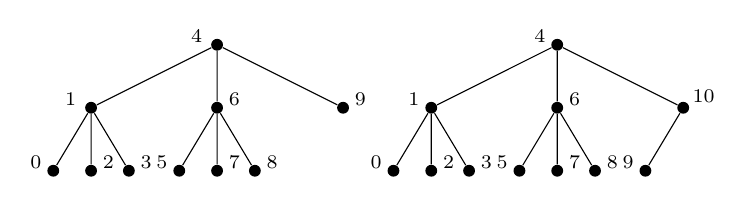
\begin{tikzpicture}[level distance=8mm, xscale = .8]
		\tikzstyle{every node}=[fill=black,circle,minimum size=.15cm,inner sep=0pt]
		\tikzstyle{every label}=[fill=none,font=\scriptsize,draw=none]
		\tikzstyle{level 1}=[sibling distance=20mm]
		\tikzstyle{level 2}=[sibling distance=6mm]
		\tikzstyle{level 3}=[sibling distance=6mm]
    \def\x{.6mm}

		\node[label={[label distance=1mm]170:
			{\nodeindex{4}}
		}] {}
		child {node[label={[label distance=1mm]170:
				{\nodeindex{1}}
			}] {}
			child {node[label={[label distance=\x]170:{\nodeindex{0}}}] {}}
			child {node[label={[label distance=\x]10:{\nodeindex{2}}}] {}}
			child {node[label={[label distance=\x]10:{\nodeindex{3}}}] {}}
		}
		child {node[label={[label distance=\x]10:
				{\nodeindex{6}}
			}] {}
			child {node[label={[label distance=\x]170:{\nodeindex{5}}}] {}}
			child {node[label={[label distance=\x]10:{\nodeindex{7}}}] {}}
			child {node[label={[label distance=\x]10:{\nodeindex{8}}}] {}}
		}
    child {node[label={[label distance=\x]10:
				{\nodeindex{9}}
			}] {}
		};
    \node[label={[label distance=\x]170:
			{\nodeindex{4}}
		}] at (5.4,0) {}
		child {node[label={[label distance=\x]170:
				{\nodeindex{1}}
			}] {}
			child {node[label={[label distance=\x]170:{\nodeindex{0}}}] {}}
			child {node[label={[label distance=\x]10:{\nodeindex{2}}}] {}}
			child {node[label={[label distance=\x]10:{\nodeindex{3}}}] {}}
		}
		child {node[label={[label distance=\x]10:
				{\nodeindex{6}}
			}] {}
			child {node[label={[label distance=\x]170:{\nodeindex{5}}}] {}}
			child {node[label={[label distance=\x]10:{\nodeindex{7}}}] {}}
			child {node[label={[label distance=\x]10:{\nodeindex{8}}}] {}}
		}
    child {node[label={[label distance=\x]10:
				{\nodeindex{10}}
			}] {}
      child {node[label={[label distance=\x]170:{\nodeindex{9}}}] {}}
      child {node[fill=none] {} edge from parent[draw=none]}
      child {node[fill=none] {} edge from parent[draw=none]}
		};
	\end{tikzpicture}
	\caption{The trees $\lbt{3}{7}$ (left) and $\lbt{3}{8}$ (right) with node indices.}
	\label{fig:lbbtex}
\end{figure}

\begin{definition}[$\addleaf$]\label{def:addleaf}
	The algorithm $\addleaf(\tree, v)$ takes as input a $\treeArity$-ary tree $\tree$ with root $r$ and $n$ nodes, and a fresh leaf $v$ and returns a new tree $\tree'$ with $v$ inserted and $v.\nodeIndex=n+1$.
	\begin{enumerate}[label=\alph*),itemsep=0pt]
    \item If $\tree$ is full, then create a new root $r'$ for $\tree'$. Attach $r$ as the first child of $r'$ and $v$ as the second child.
    \item Else if $r.\children$ contains only nodes with full subtrees, let $\tree'=\tree$ except $v$ is attached as the next child of $r$.
    \item Else, let $u$ be the first in $r.\children$ s.t. its subtree $\tree_u$ is not full. Let $\tree'=\tree$ except $\tree_u$ is replaced by $\addleaf(\tree_u,v)$.
	\end{enumerate}
\end{definition}

The following lemma formalizes the correctness of $\addleaf$. We prove it in \cref{sec:addleafprf}.
\begin{restatable}{theorem}{addleafLem}\label{lemm:addleaf}
	$\tree = \lbt{\treeArity}{n} \implies \addleaf(\tree, v) = \lbt{\treeArity}{n+1}$.
\end{restatable}

\begin{proof}
  The proof is by strong induction on $n$. If $n<\treeArity$, then the statement easily follows by inspection (only cases a) and b) of $\addleaf$ apply).
  Fix $n\geq\treeArity$ and assume the statement holds for all $k<n$. Let $r$ be the root of $\tree$ and let $\mpow(n) = \max\{\treeArity^p + 1 : p \in \N \land \treeArity^p < n\}$.

  If $\tree$ is full, then $\mpow(n+1)=n$. Furthermore, the root of $\tree'$ has only two children: $\tree=\lbt{\treeArity}{n} = \lbt{\treeArity}{\mpow(n+1)}$ and $\lbt{\treeArity}{1}$, so $\tree'=\lbt{\treeArity}{n+1}$ per definition.

  Else, $\mpow(n)=\mpow(n+1)$ (this holds since $n\geq\treeArity$). Moreover, it is easy to see that only the last node in $r.\children$ can be non-full. This means that the root $r'$ of $\tree'$ has the following children (in order):
  \begin{itemize}
    \item All children of the root $r$ of $\tree$ which have full subtrees. These subtrees are equal to $\lbt{\treeArity}{\mpow(n)}$ which is the same as $\lbt{\treeArity}{\mpow(n+1)}$.
    \item If $r$ has no non-full subtrees, then the last child of $r'$ is $v$ with subtree $\lbt{\treeArity}{1}$.
    \item Else if the last child $u$ of $r$ is non-full and equals to $\lbt{\treeArity}{x}$ for $x<\mpow(n)$, then the last child of $r'$ is $\lbt{\treeArity}{x+1}$ by induction hypothesis.
  \end{itemize}
  Clearly, $\tree'=\lbt{\treeArity}{n+1}$ in all cases.
\end{proof}


\end{document}

%%% Local Variables:
%%% mode: latex
%%% TeX-master: t
%%% End:
